%!TEX root = JournalChapter1.tex
\section{Investigating Retrieval Model Problems}
\label{RMinvestigation}
%In this section we will study problems in state of the art retrieval models when utilised in the context of microblogs.
The literature has identified \textbf{document length normalization} as the main culprit for the under-performance of retrieval efforts in microblogs. The work by \cite{naveed2011searching} suggests that the \textbf{Verbosity} and \textbf{Scope} hypotheses do not hold for microblog retrieval.

The \textbf{verbosity} hypothesis supports that some authors are more verbose than others, thus applying length normalization by dividing by the length of the document is beneficial to better capture relevance, as repetition of terms is superfluous. On the other hand, the \textbf{scope} hypotheses states that some authors simply have more to say, thus naturally adding more relevant information to the topic. As a result documents are longer but more extensive and rigorous in their content than shorter ones. The added value should be accounted for and thus the documents should promoted over shorter ones should not be normalised w.r.t their length.

In the context of Microblog retrieval, \cite{naveed2011searching} carried out a number of experiments using a logistic regression model over a number of tweet features as the retrieval methodology. They showed significant improvements in performance when their algorithm did not perform document length normalization over its normalised counterpart. However, since in their work their ranking approach takes into consideration multiple other features, it is not clear if their finding about document length normalization is generalisable.

Furthermore, although it is been often assumed, it is not known if length normalisation is bad altogether for microblog retrieval, or maybe is just how it is interpreted in this particular case what makes it harmful.

Intuition tell us that document length normalization as we know it does not interact well with the limitations characterised by microblogs. The \textbf{Verbosity} and \textbf{Scope} hypotheses seem not to model the behaviour of users publishing microblogs. Microblog users generally have the challenge of fitting their messages within the strict character limit. Consequently, retrieval models designed under scope and verbosity or similar premises, such as BM25 \cite{robertson2009probabilistic} are likely to exhibit unexpected behaviour.

To aid in developing our understanding of the behaviour of retrieval models we formalise their composition. To this end we have compiled Table \ref{modelfeatures} to show the different components involved in the score computation of a variety of state of the art retrieval models. The top row of the table indicates whether the component relies on collection statistics (I.e. Collection feature) or the document itself (Document feature). The second row contains acronyms for each of the features, which are expanded as: 

\begin{itemize}
\item [$\bullet$] \textbf{AverageDocumentLength (ADL):} This is the average document length, in number of tokens, for the whole collection.
\item [$\bullet$] \textbf{DocumentLength (DL):} This is the document length, in number of tokens, for the document being scored.
%% what about key frequency (shouldnt matter, as terms appear only once in the queries, but good to mention)
%\item \textbf{KeyFrequency (KF):} This is the term frequency of the query term within the query itself.
\item [$\bullet$] \textbf{NumberOfDocuments (ND):} Total number of documents in the collection. 
\item [$\bullet$] \textbf{DocumentFrequency (DF):} Number of documents in which the term appears (I.e. A term's posting list size).
\item [$\bullet$] \textbf{NumberOfTokens (NT):} Number of different tokens in the collection.
\item [$\bullet$] \textbf{CollectionTermFrequency (CTF):} Frequency of a term in the whole collection. (I.e. Total number of occurences of a term in the collection)
\item [$\bullet$] \textbf{TermFrequency (TF):} Frequency of the term in the document being evaluated.
\end{itemize}

\begin{table}[h!]
	\caption{Features involved in the computation of retrieval models.}
	\centering
	\begin{tabular}{|l|c|c|c|c|c||c|c|} 
		\cline{2- 8}
		\multicolumn{1}{c|}{}& \multicolumn{5}{c||}{Collection Features} &  \multicolumn{2}{c|}{Document Features} \tabularnewline
		\cline{2- 8}
		\multicolumn{1}{c|}{}
		& \textit{\textbf{ND} } & \textit{\textbf{DF} } & \textit{\textbf{ADL} } & \textit{\textbf{NT} } 
		& \textit{\textbf{CTF} } & \textit{\textbf{TF} } & \textit{\textbf{DL} } \tabularnewline \hline
		\textit{IDF} 	& * &  *&  	&   &  	&	&   \tabularnewline \hline
		\textit{DFRee} 	&   &   &   & * & * &*	&* \tabularnewline \hline
		\textit{BM25}	& * &  *& * &   &  	&*	&* \tabularnewline \hline
		\textit{HLM} 	&   &   &  	& * & * &*	&* \tabularnewline \hline
		\textit{DLM} 	&   &   &  	& * & * &*	&* \tabularnewline \hline
	\end{tabular}
	\label{modelfeatures}
\end{table}

Each of the remaining rows contain the name of the retrieval model as well as whether a component involved in its computation (Denoted by *). For example, DFRee uses NumberOfTokens (NT), CollectionTermFrequency (CTF), TermFrequency (TF) and Document Length (DL).

\subsection{The BM25 Case}
\label{bm25case}
The work by \cite{ferguson2012investigation} examined the performance of BM25 when used under a microblog retrieval scenario. Their findings showed how the closer to zero the free parameters were set in BM25, the better the performance achieved. However, they did not connect this finding to the design of BM25 and what these settings meant in terms of the affected components. In this section we exemplify and connect these findings to the theory by simulating the behaviour of BM25 under microblog retrieval conditions.

% and examine how they affect other retrieval models aside from BM25.
First, we observe in Table \ref{modelfeatures} how BM25 relies on document length by using both ADL and DL components in its computation. Furthermore, BM25 has two free parameters, namely \(b\) and \(k_1\), which control the effects of the ``saturation function'' over the final score. The saturation function in BM25 encodes the document length evidence as part of the score as follows: 

The first version of the saturation function is given by:

\begin{equation}
 \text{Version 1: }\frac{f(q_i, D)}{f(q_i, D) + k_1} \text{   for some k_1 $>$ 0}
\end{equation}

Once we take into consideration the Verbosity and Scope hypotheses, we derive the following saturation function:

\begin{equation}
 \text{Version 2: }\frac{f(q_i, D)}{f(q_i, D) + k_1*((1-b)+b*dl/avdl)} \text{   for some k_1 $>$ 0}
\end{equation}

The main difference between these equations is that \textbf{Version 2} reduces the effect of term frequency with respect to the document length and its collection average, whilst \textbf{Version 1} only relies on the \(k_1\) free parameter. Secondly, the free parameter \(b\) ponders between the Verbosity and Scope hypotheses. Setting \(b\) to 0 effectively disables the Verbose hypothesis, giving full weight to Scope, in other words, the longer the document the better. Thus when \(b\) is set to 0, \textit{Version 2} of the saturation function becomes \textit{Version 1}.

As we introduced before, the study carried by \cite{ferguson2012investigation} explored the best parameters for \(b\) and \(k_1\) concluding that best performance is achieved as both parameters tend to 0. However, the authors did not mention is that by setting those parameters close to 0, we are disregarding the document length normalisation component altogether. Thus for all intents and purposes BM25 becomes IDF. This can be proved mathematically by substituting \(b\) and \(k_1\) by 0 as follows \ref{bm25proof}.

\begin{small}
\begin{align}
\label{bm25proof}
    \notag \text{BM25}(D,Q) &= \sum_{i=1}^{n} \text{IDF}(q_i) \cdot \frac{f(q_i, D) \cdot (k_1 + 1)}{f(q_i, D) + k_1 \cdot (1 - b + b \cdot \frac{|D|}{\text{avgdl}})} \\
  \notag&= \sum_{i=1}^{n} \text{IDF}(q_i) \cdot \frac{f(q_i, D) \cdot (0 + 1)}{f(q_i, D) + 0 \cdot (1 - 0 + 0 \cdot \frac{|D|}{\text{avgdl}})} \\
  \notag&= \sum_{i=1}^{n} \text{IDF}(q_i) \cdot \frac{f(q_i, D)}{f(q_i, D) } \\
  &= \sum_{i=1}^{n} \text{IDF}(q_i)              
\end{align}
%\end{proof}
\end{small}

Initially it would seem that the \textbf{Scope} and \textbf{Verbosity} hypotheses do not hold for microblogs. The reasoning behind being that these hypotheses were developed for documents that were unbounded in terms of their length such as web pages or books. However, since document length has an upper bound in microblogs, authors express their ideas in a very constrained space where verbosity and scope hypotheses do not seem to hold. However we will later observe that this conclusion is partially true\footnote{We later demonstrate that \textbf{scope} does hold, but not \textbf{verbosity}}.

\begin{figure}[]
  \centering
   
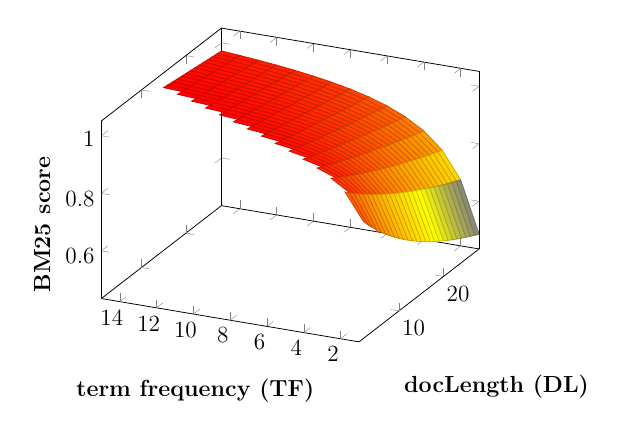
\begin{tikzpicture}[thick,scale=0.7, every node/.style={transform shape}]\begin{axis}[
 %title={},
 %y dir=reverse, 
 x dir=reverse, 
 ylabel={docLength (DL)},
 xlabel={term frequency (TF)},
 zlabel={BM25 score},
 every axis/.append style={font=\large\bfseries},
 max space between ticks=25pt
 view={55}{80}
% yticklabels={0k,100k}
 ] 

\addplot3[surf,unbounded coords=jump] coordinates { 
%patch,patch type=biquadratic, shader=faceted,patch refines=3
(1,1,0.865013774104683)	(2,1,nan)	(3,1,nan)	(4,1,nan)	(5,1,nan)	(6,1,nan)	(7,1,nan)	(8,1,nan)	(9,1,nan)	(10,1,nan)	(11,1,nan)	(12,1,nan)	(13,1,nan)	(14,1,nan)	(15,1,nan)

(1,2,0.840696117804551)	(2,2,0.932442464736451)	(3,2,nan)	(4,2,nan)	(5,2,nan)	(6,2,nan)	(7,2,nan)	(8,2,nan)	(9,2,nan)	(10,2,nan)	(11,2,nan)	(12,2,nan)	(13,2,nan)	(14,2,nan)	(15,2,nan)

(1,3,0.817708333333333)	(2,3,0.91812865497076)	(3,3,0.957317073170732)	(4,3,nan)	(5,3,nan)	(6,3,nan)	(7,3,nan)	(8,3,nan)	(9,3,nan)	(10,3,nan)	(11,3,nan)	(12,3,nan)	(13,3,nan)	(14,3,nan)	(15,3,nan)

(1,4,0.79594423320659)	(2,4,0.904247660187184)	(3,4,0.947209653092005)	(4,4,0.970258787176516)	(5,4,nan)	(6,4,nan)	(7,4,nan)	(8,4,nan)	(9,4,nan)	(10,4,nan)	(11,4,nan)	(12,4,nan)	(13,4,nan)	(14,4,nan)	(15,4,nan)

(1,5,0.775308641975309)	(2,5,0.890780141843972)	(3,5,0.937313432835821)	(4,5,0.962452107279693)	(5,5,0.978193146417446)	(6,5,nan)	(7,5,nan)	(8,5,nan)	(9,5,nan)	(10,5,nan)	(11,5,nan)	(12,5,nan)	(13,5,nan)	(14,5,nan)	(15,5,nan)

(1,6,0.755716004813477)	(2,6,0.87770789657582)	(3,6,0.927621861152142)	(4,6,0.95477004941087)	(5,6,0.971835345094398)	(6,6,0.98355520751762)	(7,6,nan)	(8,6,nan)	(9,6,nan)	(10,6,nan)	(11,6,nan)	(12,6,nan)	(13,6,nan)	(14,6,nan)	(15,6,nan)

(1,7,0.737089201877934)	(2,7,0.865013774104683)	(3,7,0.91812865497076)	(4,7,0.947209653092005)	(5,7,0.965559655596556)	(6,7,0.978193146417446)	(7,7,0.987421383647798)	(8,7,nan)	(9,7,nan)	(10,7,nan)	(11,7,nan)	(12,7,nan)	(13,7,nan)	(14,7,nan)	(15,7,nan)

(1,8,0.719358533791524)	(2,8,0.852681602172437)	(3,8,0.908827785817656)	(4,8,0.939768050879162)	(5,8,0.959364497402994)	(6,8,0.972889233152595)	(7,8,0.982785602503913)	(8,8,0.990341021092055)	(9,8,nan)	(10,8,nan)	(11,8,nan)	(12,8,nan)	(13,8,nan)	(14,8,nan)	(15,8,nan)

(1,9,0.702460850111857)	(2,9,0.840696117804551)	(3,9,0.899713467048711)	(4,9,0.932442464736451)	(5,9,0.953248330297511)	(6,9,0.967642526964561)	(7,9,0.978193146417446)	(8,9,0.986258343148802)	(9,9,0.992623814541623)	(10,9,nan)	(11,9,nan)	(12,9,nan)	(13,9,nan)	(14,9,nan)	(15,9,nan)

(1,10,0.686338797814207)	(2,10,0.829042904290429)	(3,10,0.890780141843972)	(4,10,0.925230202578269)	(5,10,0.947209653092005)	(6,10,0.962452107279693)	(7,10,0.973643410852713)	(8,10,0.982209188660801)	(9,10,0.988976377952755)	(10,10,0.9944576405384)	(11,10,nan)	(12,10,nan)	(13,10,nan)	(14,10,nan)	(15,10,nan)

(1,11,0.670940170940171)	(2,11,0.817708333333333)	(3,11,0.882022471910112)	(4,11,0.91812865497076)	(5,11,0.941247002398082)	(6,11,0.957317073170732)	(7,11,0.969135802469136)	(8,11,0.978193146417446)	(9,11,0.985355648535565)	(10,11,0.991161616161616)	(11,11,0.995963091118801)	(12,11,nan)	(13,11,nan)	(14,11,nan)	(15,11,nan)

(1,12,0.656217345872518)	(2,12,0.806679511881823)	(3,12,0.873435326842837)	(4,12,0.911135291984041)	(5,12,0.935358951444742)	(6,12,0.952236542835481)	(7,12,0.964669738863287)	(8,12,0.974209811906147)	(9,12,0.981761334028139)	(10,12,0.987887368255466)	(11,12,0.992956734224522)	(12,12,0.997221119491862)	(13,12,nan)	(14,12,nan)	(15,12,nan)

(1,13,0.642126789366053)	(2,13,0.79594423320659)	(3,13,0.865013774104683)	(4,13,0.904247660187184)	(5,13,0.929544108940201)	(6,13,0.947209653092005)	(7,13,0.960244648318043)	(8,13,0.970258787176516)	(9,13,0.978193146417446)	(10,13,0.984634681718407)	(11,13,0.989968472341645)	(12,13,0.9944576405384)	(13,13,0.998288089997554)	(14,13,nan)	(15,13,nan)

(1,14,0.628628628628628)	(2,14,0.785490931832395)	(3,14,0.856753069577081)	(4,14,0.897463379778491)	(5,14,0.923801117975875)	(6,14,0.942235558889722)	(7,14,0.955859969558599)	(8,14,0.966339680707828)	(9,14,0.97465080186239)	(10,14,0.981403344272543)	(11,14,0.986998142591798)	(12,14,0.991709435452033)	(13,14,0.995731186730088)	(14,14,0.99920445505171)	(15,14,nan)

(1,15,0.615686274509804)	(2,15,0.775308641975309)	(3,15,0.848648648648648)	(4,15,0.890780141843972)	(5,15,0.91812865497076)	(6,15,0.937313432835821)	(7,15,0.951515151515151)	(8,15,0.962452107279693)	(9,15,0.971134020618556)	(10,15,0.978193146417446)	(11,15,0.984045584045584)	(12,15,0.988976377952755)	(13,15,0.993187347931874)	(14,15,0.996825396825397)	(15,15,1)

(1,16,0.603266090297791)	(2,16,0.765386959171236)	(3,16,0.840696117804551)	(4,16,0.884195705737416)	(5,16,0.91252542865446)	(6,16,0.932442464736451)	(7,16,0.947209653092005)	(8,16,0.95859568784583)	(9,16,0.967642526964561)	(10,16,0.975003881384878)	(11,16,0.981110637693509)	(12,16,0.986258343148802)	(13,16,0.990656473728916)	(14,16,0.9944576405384)	(15,16,0.997775659358118)

(1,17,0.591337099811676)	(2,17,0.755716004813477)	(3,17,0.832891246684349)	(4,17,0.87770789657582)	(5,17,0.906990179087232)	(6,17,0.927621861152142)	(7,17,0.942942942942943)	(8,17,0.95477004941087)	(9,17,0.96417604912999)	(10,17,0.971835345094398)	(11,17,0.978193146417446)	(12,17,0.98355520751762)	(13,17,0.988138465262648)	(14,17,0.992101105845181)	(15,17,0.995561192136969)

(1,18,0.579870729455217)	(2,18,0.746286393345217)	(3,18,0.825229960578186)	(4,18,0.87131460284426)	(5,18,0.901521676715475)	(6,18,0.922850844966936)	(7,18,0.938714499252616)	(8,18,0.950974824910089)	(9,18,0.960734319224884)	(10,18,0.968687336109825)	(11,18,0.975292954962587)	(12,18,0.980866848887153)	(13,18,0.985633224677049)	(14,18,0.989755713159969)	(15,18,0.993356532742803)

(1,19,0.568840579710145)	(2,19,0.737089201877934)	(3,19,0.817708333333333)	(4,19,0.865013774104683)	(5,19,0.896118721461187)	(6,19,0.91812865497076)	(7,19,0.934523809523809)	(8,19,0.947209653092005)	(9,19,0.957317073170732)	(10,19,0.965559655596556)	(11,19,0.972409909909909)	(12,19,0.978193146417446)	(13,19,0.983140655105973)	(14,19,0.987421383647798)	(15,19,0.991161616161616)

(1,20,0.558222222222222)	(2,20,0.728115942028985)	(3,20,0.810322580645161)	(4,20,0.858803418803419)	(5,20,0.890780141843972)	(6,20,0.913454545454545)	(7,20,0.93037037037037)	(8,20,0.943474178403755)	(9,20,0.95392405063291)	(10,20,0.962452107279693)	(11,20,0.969543859649122)	(12,20,0.975533980582524)	(13,20,0.980660660660661)	(14,20,0.985098039215686)	(15,20,0.988976377952755)

(1,21,0.547993019197208)	(2,21,0.719358533791524)	(3,21,0.803069053708439)	(4,21,0.852681602172437)	(5,21,0.885504794134235)	(6,21,0.908827785817656)	(7,21,0.926253687315634)	(8,21,0.939768050879162)	(9,21,0.950554994954591)	(10,21,0.959364497402994)	(11,21,0.966694654352085)	(12,21,0.972889233152595)	(13,21,0.978193146417446)	(14,21,0.982785602503913)	(15,21,0.986800754242615)

(1,22,0.538131962296487)	(2,22,0.710809281267685)	(3,22,0.79594423320659)	(4,22,0.84664644421975)	(5,22,0.880291561536304)	(6,22,0.904247660187184)	(7,22,0.922173274596182)	(8,22,0.936090926029439)	(9,22,0.947209653092005)	(10,22,0.956296634688594)	(11,22,0.9638621459467)	(12,22,0.970258787176516)	(13,22,0.975738018405641)	(14,22,0.980483996877439)	(15,22,0.984634681718407)

(1,23,0.528619528619528)	(2,23,0.702460850111857)	(3,23,0.78894472361809)	(4,23,0.840696117804551)	(5,23,0.875139353400222)	(6,23,0.899713467048711)	(7,23,0.91812865497076)	(8,23,0.932442464736451)	(9,23,0.943887775551102)	(10,23,0.953248330297511)	(11,23,0.961046188091263)	(12,23,0.967642526964561)	(13,23,0.973295183595613)	(14,23,0.978193146417446)	(15,23,0.982478097622027)

(1,24,0.519437551695616)	(2,24,0.694306246545052)	(3,24,0.782067247820672)	(4,24,0.834828846792954)	(5,24,0.870047104461069)	(6,24,0.895224518888096)	(7,24,0.914119359534206)	(8,24,0.928822333148456)	(9,24,0.940589116325512)	(10,24,0.950219397790891)	(11,24,0.958246636149258)	(12,24,0.965040338071456)	(13,24,0.970864549887025)	(14,24,0.975912975912976)	(15,24,0.98033093974399)

(1,25,0.510569105691057)	(2,25,0.686338797814207)	(3,25,0.775308641975309)	(4,25,0.829042904290429)	(5,25,0.865013774104683)	(6,25,0.890780141843972)	(7,25,0.910144927536232)	(8,25,0.925230202578269)	(9,25,0.937313432835821)	(10,25,0.947209653092005)	(11,25,0.955463347164592)	(12,25,0.962452107279693)	(13,25,0.968446026097272)	(14,25,0.973643410852713)	(15,25,0.978193146417446)

(1,26,0.501998401278977)	(2,26,0.678552133981632)	(3,26,0.768665850673194)	(4,26,0.823336610947231)	(5,26,0.860038345658723)	(6,26,0.886379675370501)	(7,26,0.906204906204906)	(8,26,0.921665749403778)	(9,26,0.934060485870104)	(10,26,0.944218914448954)	(11,26,0.952696179837263)	(12,26,0.95987772258311)	(13,26,0.966039521950065)	(14,26,0.97138437741686)	(15,26,0.976064656512278)

(1,27,0.493710691823899)	(2,27,0.670940170940171)	(3,27,0.762135922330097)	(4,27,0.817708333333333)	(5,27,0.855119825708061)	(6,27,0.882022471910112)	(7,27,0.902298850574712)	(8,27,0.91812865497076)	(9,27,0.930830039525691)	(10,27,0.941247002398082)	(11,27,0.94994499449945)	(12,27,0.957317073170732)	(13,27,0.963644948064211)	(14,27,0.969135802469136)	(15,27,0.97394540942928)

(1,28,0.48569218870843)	(2,28,0.663497094558901)	(3,28,0.755716004813477)	(4,28,0.812156482379566)	(5,28,0.850257243433523)	(6,28,0.87770789657582)	(7,28,0.898426323319027)	(8,28,0.914618605497906)	(9,28,0.927621861152142)	(10,28,0.938293739728074)	(11,28,0.947209653092005)	(12,28,0.95477004941087)	(13,28,0.961262215942541)	(14,28,0.966897613548883)	(15,28,0.971835345094398)



}; \end{axis} \end{tikzpicture}

     \caption{Term Frequency (TF) vs, Doc. Length (DL)}
  \label{bm25scoretfdl}
\end{figure}

Furthermore, terms in microblog documents have very low document frequencies. In fact, more often than not, query terms appear at most once in each document unless dealing with spam. Thus a query term appearing more than once within a document can have a dramatic effect over the score produced by BM25. In other words, the very low document frequencies result in unreliable estimations of the informativeness of a query term. Consequently, in this particular case, it is better to rely on features outside the document such as collection features.

Finally, Figure \ref{bm25scoretfdl} shows the possible BM25 scores for a range of Term Frequency (TF) and Doc. Length (DL) values.\footnote{Where \(ND=100k\) and \(DF=100\)}. We can extract two interesting behaviours which we can compare later to other retrieval models. Firstly the increase of document length is regarded as negative. In other words the more information in number of terms is encoded in the document the less relevant it is regarded. Secondly the increasing term frequency results in increased scores. This would seem counter-intuitive in a document with such a limited length, as users normally struggle to fit their messages. Additionally, there is a danger of promoting spam messages which may only contain the query terms.


%\mentalnote{Finally, by reducing the values of the b and k constants, the standard deviation of across the scores (w.r.t. tf and dl) by bm25 is also reduced, reaching 0 when b and k are 0, as tf and dl do not play any role in this case. Lower stdev. better performance}

\subsection{The Hiemstra's Language Model (HLM) Case}
%Now we study the Hiemstra's Language Model (HLM) under Microblog conditions. 
Table \ref{modelfeatures} shows that HLM utilises both CollectionTermFrequency (CTF) and TermFrequency (TF) together with the total number of different tokens in the collection (NT) and document length (DL). Furthermore, if we pay attention to Table \ref{traditional} we can observe that whilst DFR and HLM utilize the same components, HLM exhibits a more erratic performance under microblog conditions. HLM's performance for the 2013 collection is considerably lower than that of DFR or IDF, whereas it remains close to the top performing models for the 2011, 2012 and 2014 collections. HLM is formulated as follows: 

\begin{small}
\begin{align}
\label{hlmformula}
    \text{HLM}(D,Q) &= \sum_{i=1}^{n} \log_2 \left[ 1 + \frac{c \cdot f(q_i, D) \cdot ntoks }{ (1-c) \cdot f(q_i, C) \cdot |D|} \right]
\end{align}
\end{small}

where $ntoks$ refers to the number of unique tokens in the collection (NT), $c$ is a free parameter, and $C$ represents the set of all documents in the collection. $f(q_i, D)$ represents the TF of a query term $q_i$ in document $D$, whereas $f(q_i, C)$ is CTF of term $q_i$. The free parameter c regulates how HLM satisfies the conditions of \textbf{coordination level ranking (CLR)}) \cite{hiemstra2000relating}. CLR is a rule enforced in the design of HLM which ensures that documents containing $n$ query terms are ranked higher than those with $n-1$ terms.

%\begin{figure}[]
%%        
%%       \begin{subfigure}[b]{0.5\textwidth}
%%        \centering
%%        \caption{Doc. Frequency (CTF) vs, $c$}
%%         
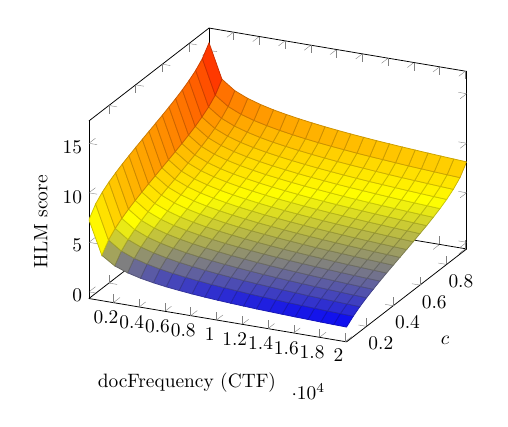
\begin{tikzpicture}[thick,scale=0.7, every node/.style={transform shape}]\begin{axis}[
 %title={},
 %y dir=reverse, 
 %x dir=reverse, 
 ylabel={$c$},
 xlabel={docFrequency (CTF)},
 zlabel={HLM score},
 max space between ticks=16pt
% yticklabels={0k,100k}
 ] 

		\addplot3[surf] coordinates { 
%patch,patch type=biquadratic, shader=faceted,patch refines=3

(100.00,0.05,7.28)(100.00,0.10,8.35)(100.00,0.15,9.02)(100.00,0.20,9.52)(100.00,0.25,9.93)(100.00,0.30,10.30)(100.00,0.35,10.62)(100.00,0.40,10.93)(100.00,0.45,11.23)(100.00,0.50,11.52)(100.00,0.55,11.81)(100.00,0.60,12.10)(100.00,0.65,12.41)(100.00,0.70,12.74)(100.00,0.75,13.10)(100.00,0.80,13.52)(100.00,0.85,14.02)(100.00,0.90,14.69)(100.00,0.95,15.76)

(1100.00,0.05,3.91)(1100.00,0.10,4.94)(1100.00,0.15,5.59)(1100.00,0.20,6.08)(1100.00,0.25,6.49)(1100.00,0.30,6.85)(1100.00,0.35,7.17)(1100.00,0.40,7.48)(1100.00,0.45,7.77)(1100.00,0.50,8.06)(1100.00,0.55,8.35)(1100.00,0.60,8.65)(1100.00,0.65,8.95)(1100.00,0.70,9.28)(1100.00,0.75,9.64)(1100.00,0.80,10.06)(1100.00,0.85,10.56)(1100.00,0.90,11.23)(1100.00,0.95,12.31)

(2100.00,0.05,3.06)(2100.00,0.10,4.04)(2100.00,0.15,4.68)(2100.00,0.20,5.17)(2100.00,0.25,5.57)(2100.00,0.30,5.93)(2100.00,0.35,6.25)(2100.00,0.40,6.56)(2100.00,0.45,6.85)(2100.00,0.50,7.13)(2100.00,0.55,7.42)(2100.00,0.60,7.72)(2100.00,0.65,8.02)(2100.00,0.70,8.35)(2100.00,0.75,8.71)(2100.00,0.80,9.13)(2100.00,0.85,9.63)(2100.00,0.90,10.30)(2100.00,0.95,11.37)

(3100.00,0.05,2.58)(3100.00,0.10,3.52)(3100.00,0.15,4.14)(3100.00,0.20,4.62)(3100.00,0.25,5.02)(3100.00,0.30,5.38)(3100.00,0.35,5.70)(3100.00,0.40,6.00)(3100.00,0.45,6.29)(3100.00,0.50,6.58)(3100.00,0.55,6.86)(3100.00,0.60,7.16)(3100.00,0.65,7.46)(3100.00,0.70,7.79)(3100.00,0.75,8.15)(3100.00,0.80,8.57)(3100.00,0.85,9.07)(3100.00,0.90,9.73)(3100.00,0.95,10.81)

(4100.00,0.05,2.25)(4100.00,0.10,3.16)(4100.00,0.15,3.77)(4100.00,0.20,4.24)(4100.00,0.25,4.63)(4100.00,0.30,4.98)(4100.00,0.35,5.30)(4100.00,0.40,5.60)(4100.00,0.45,5.89)(4100.00,0.50,6.18)(4100.00,0.55,6.47)(4100.00,0.60,6.76)(4100.00,0.65,7.06)(4100.00,0.70,7.39)(4100.00,0.75,7.75)(4100.00,0.80,8.16)(4100.00,0.85,8.67)(4100.00,0.90,9.33)(4100.00,0.95,10.41)

(5100.00,0.05,2.01)(5100.00,0.10,2.88)(5100.00,0.15,3.48)(5100.00,0.20,3.94)(5100.00,0.25,4.33)(5100.00,0.30,4.68)(5100.00,0.35,5.00)(5100.00,0.40,5.30)(5100.00,0.45,5.59)(5100.00,0.50,5.87)(5100.00,0.55,6.15)(5100.00,0.60,6.45)(5100.00,0.65,6.75)(5100.00,0.70,7.08)(5100.00,0.75,7.44)(5100.00,0.80,7.85)(5100.00,0.85,8.35)(5100.00,0.90,9.02)(5100.00,0.95,10.09)

(6100.00,0.05,1.82)(6100.00,0.10,2.66)(6100.00,0.15,3.24)(6100.00,0.20,3.70)(6100.00,0.25,4.09)(6100.00,0.30,4.43)(6100.00,0.35,4.75)(6100.00,0.40,5.05)(6100.00,0.45,5.33)(6100.00,0.50,5.62)(6100.00,0.55,5.90)(6100.00,0.60,6.19)(6100.00,0.65,6.50)(6100.00,0.70,6.82)(6100.00,0.75,7.18)(6100.00,0.80,7.59)(6100.00,0.85,8.09)(6100.00,0.90,8.76)(6100.00,0.95,9.84)

(7100.00,0.05,1.67)(7100.00,0.10,2.48)(7100.00,0.15,3.05)(7100.00,0.20,3.50)(7100.00,0.25,3.88)(7100.00,0.30,4.22)(7100.00,0.35,4.54)(7100.00,0.40,4.83)(7100.00,0.45,5.12)(7100.00,0.50,5.40)(7100.00,0.55,5.69)(7100.00,0.60,5.98)(7100.00,0.65,6.28)(7100.00,0.70,6.60)(7100.00,0.75,6.96)(7100.00,0.80,7.38)(7100.00,0.85,7.88)(7100.00,0.90,8.54)(7100.00,0.95,9.62)

(8100.00,0.05,1.54)(8100.00,0.10,2.33)(8100.00,0.15,2.88)(8100.00,0.20,3.33)(8100.00,0.25,3.71)(8100.00,0.30,4.04)(8100.00,0.35,4.36)(8100.00,0.40,4.65)(8100.00,0.45,4.94)(8100.00,0.50,5.22)(8100.00,0.55,5.50)(8100.00,0.60,5.79)(8100.00,0.65,6.09)(8100.00,0.70,6.42)(8100.00,0.75,6.78)(8100.00,0.80,7.19)(8100.00,0.85,7.69)(8100.00,0.90,8.35)(8100.00,0.95,9.43)

(9100.00,0.05,1.43)(9100.00,0.10,2.19)(9100.00,0.15,2.74)(9100.00,0.20,3.18)(9100.00,0.25,3.55)(9100.00,0.30,3.89)(9100.00,0.35,4.20)(9100.00,0.40,4.49)(9100.00,0.45,4.77)(9100.00,0.50,5.05)(9100.00,0.55,5.33)(9100.00,0.60,5.62)(9100.00,0.65,5.93)(9100.00,0.70,6.25)(9100.00,0.75,6.61)(9100.00,0.80,7.02)(9100.00,0.85,7.52)(9100.00,0.90,8.18)(9100.00,0.95,9.26)

(10100.00,0.05,1.34)(10100.00,0.10,2.08)(10100.00,0.15,2.61)(10100.00,0.20,3.05)(10100.00,0.25,3.42)(10100.00,0.30,3.75)(10100.00,0.35,4.06)(10100.00,0.40,4.35)(10100.00,0.45,4.63)(10100.00,0.50,4.91)(10100.00,0.55,5.19)(10100.00,0.60,5.48)(10100.00,0.65,5.78)(10100.00,0.70,6.10)(10100.00,0.75,6.46)(10100.00,0.80,6.87)(10100.00,0.85,7.37)(10100.00,0.90,8.03)(10100.00,0.95,9.11)

(11100.00,0.05,1.26)(11100.00,0.10,1.98)(11100.00,0.15,2.50)(11100.00,0.20,2.93)(11100.00,0.25,3.29)(11100.00,0.30,3.62)(11100.00,0.35,3.93)(11100.00,0.40,4.22)(11100.00,0.45,4.50)(11100.00,0.50,4.78)(11100.00,0.55,5.06)(11100.00,0.60,5.34)(11100.00,0.65,5.64)(11100.00,0.70,5.97)(11100.00,0.75,6.33)(11100.00,0.80,6.74)(11100.00,0.85,7.23)(11100.00,0.90,7.90)(11100.00,0.95,8.97)

(12100.00,0.05,1.19)(12100.00,0.10,1.88)(12100.00,0.15,2.40)(12100.00,0.20,2.82)(12100.00,0.25,3.18)(12100.00,0.30,3.51)(12100.00,0.35,3.81)(12100.00,0.40,4.10)(12100.00,0.45,4.38)(12100.00,0.50,4.66)(12100.00,0.55,4.94)(12100.00,0.60,5.22)(12100.00,0.65,5.52)(12100.00,0.70,5.85)(12100.00,0.75,6.20)(12100.00,0.80,6.61)(12100.00,0.85,7.11)(12100.00,0.90,7.77)(12100.00,0.95,8.85)

(13100.00,0.05,1.12)(13100.00,0.10,1.80)(13100.00,0.15,2.31)(13100.00,0.20,2.72)(13100.00,0.25,3.08)(13100.00,0.30,3.40)(13100.00,0.35,3.71)(13100.00,0.40,3.99)(13100.00,0.45,4.27)(13100.00,0.50,4.55)(13100.00,0.55,4.82)(13100.00,0.60,5.11)(13100.00,0.65,5.41)(13100.00,0.70,5.73)(13100.00,0.75,6.09)(13100.00,0.80,6.50)(13100.00,0.85,7.00)(13100.00,0.90,7.66)(13100.00,0.95,8.73)

(14100.00,0.05,1.07)(14100.00,0.10,1.73)(14100.00,0.15,2.22)(14100.00,0.20,2.63)(14100.00,0.25,2.99)(14100.00,0.30,3.31)(14100.00,0.35,3.61)(14100.00,0.40,3.89)(14100.00,0.45,4.17)(14100.00,0.50,4.45)(14100.00,0.55,4.72)(14100.00,0.60,5.01)(14100.00,0.65,5.31)(14100.00,0.70,5.63)(14100.00,0.75,5.99)(14100.00,0.80,6.39)(14100.00,0.85,6.89)(14100.00,0.90,7.56)(14100.00,0.95,8.63)

(15100.00,0.05,1.02)(15100.00,0.10,1.66)(15100.00,0.15,2.15)(15100.00,0.20,2.55)(15100.00,0.25,2.90)(15100.00,0.30,3.22)(15100.00,0.35,3.52)(15100.00,0.40,3.80)(15100.00,0.45,4.08)(15100.00,0.50,4.35)(15100.00,0.55,4.63)(15100.00,0.60,4.91)(15100.00,0.65,5.21)(15100.00,0.70,5.53)(15100.00,0.75,5.89)(15100.00,0.80,6.30)(15100.00,0.85,6.79)(15100.00,0.90,7.46)(15100.00,0.95,8.53)

(16100.00,0.05,0.97)(16100.00,0.10,1.60)(16100.00,0.15,2.07)(16100.00,0.20,2.47)(16100.00,0.25,2.82)(16100.00,0.30,3.14)(16100.00,0.35,3.43)(16100.00,0.40,3.72)(16100.00,0.45,3.99)(16100.00,0.50,4.26)(16100.00,0.55,4.54)(16100.00,0.60,4.82)(16100.00,0.65,5.12)(16100.00,0.70,5.44)(16100.00,0.75,5.80)(16100.00,0.80,6.21)(16100.00,0.85,6.70)(16100.00,0.90,7.36)(16100.00,0.95,8.44)

(17100.00,0.05,0.93)(17100.00,0.10,1.54)(17100.00,0.15,2.01)(17100.00,0.20,2.40)(17100.00,0.25,2.75)(17100.00,0.30,3.06)(17100.00,0.35,3.35)(17100.00,0.40,3.64)(17100.00,0.45,3.91)(17100.00,0.50,4.18)(17100.00,0.55,4.46)(17100.00,0.60,4.74)(17100.00,0.65,5.04)(17100.00,0.70,5.36)(17100.00,0.75,5.71)(17100.00,0.80,6.12)(17100.00,0.85,6.62)(17100.00,0.90,7.28)(17100.00,0.95,8.35)

(18100.00,0.05,0.89)(18100.00,0.10,1.48)(18100.00,0.15,1.95)(18100.00,0.20,2.34)(18100.00,0.25,2.68)(18100.00,0.30,2.99)(18100.00,0.35,3.28)(18100.00,0.40,3.56)(18100.00,0.45,3.83)(18100.00,0.50,4.10)(18100.00,0.55,4.38)(18100.00,0.60,4.66)(18100.00,0.65,4.96)(18100.00,0.70,5.28)(18100.00,0.75,5.63)(18100.00,0.80,6.04)(18100.00,0.85,6.54)(18100.00,0.90,7.20)(18100.00,0.95,8.27)

(19100.00,0.05,0.85)(19100.00,0.10,1.44)(19100.00,0.15,1.89)(19100.00,0.20,2.27)(19100.00,0.25,2.61)(19100.00,0.30,2.92)(19100.00,0.35,3.21)(19100.00,0.40,3.49)(19100.00,0.45,3.76)(19100.00,0.50,4.03)(19100.00,0.55,4.30)(19100.00,0.60,4.59)(19100.00,0.65,4.88)(19100.00,0.70,5.20)(19100.00,0.75,5.56)(19100.00,0.80,5.96)(19100.00,0.85,6.46)(19100.00,0.90,7.12)(19100.00,0.95,8.19)

(20100.00,0.05,0.82)(20100.00,0.10,1.39)(20100.00,0.15,1.84)(20100.00,0.20,2.22)(20100.00,0.25,2.55)(20100.00,0.30,2.86)(20100.00,0.35,3.15)(20100.00,0.40,3.42)(20100.00,0.45,3.69)(20100.00,0.50,3.96)(20100.00,0.55,4.23)(20100.00,0.60,4.52)(20100.00,0.65,4.81)(20100.00,0.70,5.13)(20100.00,0.75,5.48)(20100.00,0.80,5.89)(20100.00,0.85,6.39)(20100.00,0.90,7.05)(20100.00,0.95,8.12)
%
%(21100.00,0.05,0.79)(21100.00,0.10,1.35)(21100.00,0.15,1.79)(21100.00,0.20,2.16)(21100.00,0.25,2.49)(21100.00,0.30,2.80)(21100.00,0.35,3.08)(21100.00,0.40,3.36)(21100.00,0.45,3.63)(21100.00,0.50,3.90)(21100.00,0.55,4.17)(21100.00,0.60,4.45)(21100.00,0.65,4.74)(21100.00,0.70,5.06)(21100.00,0.75,5.42)(21100.00,0.80,5.82)(21100.00,0.85,6.32)(21100.00,0.90,6.98)(21100.00,0.95,8.05)
%
%(22100.00,0.05,0.76)(22100.00,0.10,1.31)(22100.00,0.15,1.74)(22100.00,0.20,2.11)(22100.00,0.25,2.44)(22100.00,0.30,2.74)(22100.00,0.35,3.03)(22100.00,0.40,3.30)(22100.00,0.45,3.57)(22100.00,0.50,3.83)(22100.00,0.55,4.10)(22100.00,0.60,4.38)(22100.00,0.65,4.68)(22100.00,0.70,5.00)(22100.00,0.75,5.35)(22100.00,0.80,5.76)(22100.00,0.85,6.25)(22100.00,0.90,6.91)(22100.00,0.95,7.98)
%
%(23100.00,0.05,0.74)(23100.00,0.10,1.27)(23100.00,0.15,1.70)(23100.00,0.20,2.06)(23100.00,0.25,2.39)(23100.00,0.30,2.69)(23100.00,0.35,2.97)(23100.00,0.40,3.24)(23100.00,0.45,3.51)(23100.00,0.50,3.77)(23100.00,0.55,4.04)(23100.00,0.60,4.32)(23100.00,0.65,4.62)(23100.00,0.70,4.94)(23100.00,0.75,5.29)(23100.00,0.80,5.69)(23100.00,0.85,6.19)(23100.00,0.90,6.85)(23100.00,0.95,7.92)
%
%(24100.00,0.05,0.71)(24100.00,0.10,1.23)(24100.00,0.15,1.65)(24100.00,0.20,2.01)(24100.00,0.25,2.34)(24100.00,0.30,2.63)(24100.00,0.35,2.92)(24100.00,0.40,3.19)(24100.00,0.45,3.45)(24100.00,0.50,3.72)(24100.00,0.55,3.99)(24100.00,0.60,4.27)(24100.00,0.65,4.56)(24100.00,0.70,4.88)(24100.00,0.75,5.23)(24100.00,0.80,5.63)(24100.00,0.85,6.13)(24100.00,0.90,6.79)(24100.00,0.95,7.86)
%
%(25100.00,0.05,0.69)(25100.00,0.10,1.20)(25100.00,0.15,1.61)(25100.00,0.20,1.97)(25100.00,0.25,2.29)(25100.00,0.30,2.59)(25100.00,0.35,2.87)(25100.00,0.40,3.13)(25100.00,0.45,3.40)(25100.00,0.50,3.66)(25100.00,0.55,3.93)(25100.00,0.60,4.21)(25100.00,0.65,4.50)(25100.00,0.70,4.82)(25100.00,0.75,5.17)(25100.00,0.80,5.58)(25100.00,0.85,6.07)(25100.00,0.90,6.73)(25100.00,0.95,7.80)
%
%(26100.00,0.05,0.67)(26100.00,0.10,1.17)(26100.00,0.15,1.58)(26100.00,0.20,1.93)(26100.00,0.25,2.25)(26100.00,0.30,2.54)(26100.00,0.35,2.82)(26100.00,0.40,3.08)(26100.00,0.45,3.35)(26100.00,0.50,3.61)(26100.00,0.55,3.88)(26100.00,0.60,4.16)(26100.00,0.65,4.45)(26100.00,0.70,4.77)(26100.00,0.75,5.12)(26100.00,0.80,5.52)(26100.00,0.85,6.01)(26100.00,0.90,6.67)(26100.00,0.95,7.74)
%
%(27100.00,0.05,0.65)(27100.00,0.10,1.14)(27100.00,0.15,1.54)(27100.00,0.20,1.89)(27100.00,0.25,2.20)(27100.00,0.30,2.49)(27100.00,0.35,2.77)(27100.00,0.40,3.04)(27100.00,0.45,3.30)(27100.00,0.50,3.56)(27100.00,0.55,3.83)(27100.00,0.60,4.11)(27100.00,0.65,4.40)(27100.00,0.70,4.71)(27100.00,0.75,5.06)(27100.00,0.80,5.47)(27100.00,0.85,5.96)(27100.00,0.90,6.62)(27100.00,0.95,7.69)
%
%(28100.00,0.05,0.63)(28100.00,0.10,1.11)(28100.00,0.15,1.51)(28100.00,0.20,1.85)(28100.00,0.25,2.16)(28100.00,0.30,2.45)(28100.00,0.35,2.73)(28100.00,0.40,2.99)(28100.00,0.45,3.25)(28100.00,0.50,3.51)(28100.00,0.55,3.78)(28100.00,0.60,4.06)(28100.00,0.65,4.35)(28100.00,0.70,4.66)(28100.00,0.75,5.01)(28100.00,0.80,5.42)(28100.00,0.85,5.91)(28100.00,0.90,6.57)(28100.00,0.95,7.64)
%
%(29100.00,0.05,0.61)(29100.00,0.10,1.08)(29100.00,0.15,1.47)(29100.00,0.20,1.81)(29100.00,0.25,2.12)(29100.00,0.30,2.41)(29100.00,0.35,2.68)(29100.00,0.40,2.95)(29100.00,0.45,3.21)(29100.00,0.50,3.47)(29100.00,0.55,3.73)(29100.00,0.60,4.01)(29100.00,0.65,4.30)(29100.00,0.70,4.61)(29100.00,0.75,4.96)(29100.00,0.80,5.37)(29100.00,0.85,5.86)(29100.00,0.90,6.52)(29100.00,0.95,7.59)
%
%(30100.00,0.05,0.60)(30100.00,0.10,1.06)(30100.00,0.15,1.44)(30100.00,0.20,1.78)(30100.00,0.25,2.09)(30100.00,0.30,2.37)(30100.00,0.35,2.64)(30100.00,0.40,2.91)(30100.00,0.45,3.16)(30100.00,0.50,3.42)(30100.00,0.55,3.69)(30100.00,0.60,3.96)(30100.00,0.65,4.25)(30100.00,0.70,4.57)(30100.00,0.75,4.92)(30100.00,0.80,5.32)(30100.00,0.85,5.81)(30100.00,0.90,6.47)(30100.00,0.95,7.54)
%
%(31100.00,0.05,0.58)(31100.00,0.10,1.03)(31100.00,0.15,1.41)(31100.00,0.20,1.75)(31100.00,0.25,2.05)(31100.00,0.30,2.33)(31100.00,0.35,2.60)(31100.00,0.40,2.86)(31100.00,0.45,3.12)(31100.00,0.50,3.38)(31100.00,0.55,3.65)(31100.00,0.60,3.92)(31100.00,0.65,4.21)(31100.00,0.70,4.52)(31100.00,0.75,4.87)(31100.00,0.80,5.27)(31100.00,0.85,5.77)(31100.00,0.90,6.42)(31100.00,0.95,7.49)
%
%(32100.00,0.05,0.57)(32100.00,0.10,1.01)(32100.00,0.15,1.38)(32100.00,0.20,1.71)(32100.00,0.25,2.02)(32100.00,0.30,2.30)(32100.00,0.35,2.56)(32100.00,0.40,2.83)(32100.00,0.45,3.08)(32100.00,0.50,3.34)(32100.00,0.55,3.60)(32100.00,0.60,3.88)(32100.00,0.65,4.17)(32100.00,0.70,4.48)(32100.00,0.75,4.83)(32100.00,0.80,5.23)(32100.00,0.85,5.72)(32100.00,0.90,6.38)(32100.00,0.95,7.45)
%
%(33100.00,0.05,0.55)(33100.00,0.10,0.99)(33100.00,0.15,1.36)(33100.00,0.20,1.68)(33100.00,0.25,1.98)(33100.00,0.30,2.26)(33100.00,0.35,2.53)(33100.00,0.40,2.79)(33100.00,0.45,3.04)(33100.00,0.50,3.30)(33100.00,0.55,3.56)(33100.00,0.60,3.84)(33100.00,0.65,4.12)(33100.00,0.70,4.44)(33100.00,0.75,4.78)(33100.00,0.80,5.19)(33100.00,0.85,5.68)(33100.00,0.90,6.33)(33100.00,0.95,7.40)
%
%(34100.00,0.05,0.54)(34100.00,0.10,0.97)(34100.00,0.15,1.33)(34100.00,0.20,1.65)(34100.00,0.25,1.95)(34100.00,0.30,2.23)(34100.00,0.35,2.49)(34100.00,0.40,2.75)(34100.00,0.45,3.01)(34100.00,0.50,3.26)(34100.00,0.55,3.52)(34100.00,0.60,3.80)(34100.00,0.65,4.08)(34100.00,0.70,4.40)(34100.00,0.75,4.74)(34100.00,0.80,5.14)(34100.00,0.85,5.64)(34100.00,0.90,6.29)(34100.00,0.95,7.36)
%
%(35100.00,0.05,0.53)(35100.00,0.10,0.95)(35100.00,0.15,1.31)(35100.00,0.20,1.63)(35100.00,0.25,1.92)(35100.00,0.30,2.19)(35100.00,0.35,2.46)(35100.00,0.40,2.72)(35100.00,0.45,2.97)(35100.00,0.50,3.22)(35100.00,0.55,3.49)(35100.00,0.60,3.76)(35100.00,0.65,4.04)(35100.00,0.70,4.36)(35100.00,0.75,4.70)(35100.00,0.80,5.10)(35100.00,0.85,5.59)(35100.00,0.90,6.25)(35100.00,0.95,7.32)
%
%(36100.00,0.05,0.51)(36100.00,0.10,0.93)(36100.00,0.15,1.28)(36100.00,0.20,1.60)(36100.00,0.25,1.89)(36100.00,0.30,2.16)(36100.00,0.35,2.43)(36100.00,0.40,2.68)(36100.00,0.45,2.93)(36100.00,0.50,3.19)(36100.00,0.55,3.45)(36100.00,0.60,3.72)(36100.00,0.65,4.01)(36100.00,0.70,4.32)(36100.00,0.75,4.66)(36100.00,0.80,5.06)(36100.00,0.85,5.55)(36100.00,0.90,6.21)(36100.00,0.95,7.28)
%
%(37100.00,0.05,0.50)(37100.00,0.10,0.91)(37100.00,0.15,1.26)(37100.00,0.20,1.57)(37100.00,0.25,1.86)(37100.00,0.30,2.13)(37100.00,0.35,2.39)(37100.00,0.40,2.65)(37100.00,0.45,2.90)(37100.00,0.50,3.15)(37100.00,0.55,3.41)(37100.00,0.60,3.68)(37100.00,0.65,3.97)(37100.00,0.70,4.28)(37100.00,0.75,4.63)(37100.00,0.80,5.03)(37100.00,0.85,5.52)(37100.00,0.90,6.17)(37100.00,0.95,7.24)
%
%(38100.00,0.05,0.49)(38100.00,0.10,0.89)(38100.00,0.15,1.24)(38100.00,0.20,1.55)(38100.00,0.25,1.83)(38100.00,0.30,2.10)(38100.00,0.35,2.36)(38100.00,0.40,2.62)(38100.00,0.45,2.87)(38100.00,0.50,3.12)(38100.00,0.55,3.38)(38100.00,0.60,3.65)(38100.00,0.65,3.93)(38100.00,0.70,4.24)(38100.00,0.75,4.59)(38100.00,0.80,4.99)(38100.00,0.85,5.48)(38100.00,0.90,6.13)(38100.00,0.95,7.20)
%
%(39100.00,0.05,0.48)(39100.00,0.10,0.87)(39100.00,0.15,1.22)(39100.00,0.20,1.52)(39100.00,0.25,1.81)(39100.00,0.30,2.07)(39100.00,0.35,2.33)(39100.00,0.40,2.58)(39100.00,0.45,2.83)(39100.00,0.50,3.09)(39100.00,0.55,3.34)(39100.00,0.60,3.61)(39100.00,0.65,3.90)(39100.00,0.70,4.21)(39100.00,0.75,4.55)(39100.00,0.80,4.95)(39100.00,0.85,5.44)(39100.00,0.90,6.10)(39100.00,0.95,7.16)
%
%(40100.00,0.05,0.47)(40100.00,0.10,0.86)(40100.00,0.15,1.20)(40100.00,0.20,1.50)(40100.00,0.25,1.78)(40100.00,0.30,2.05)(40100.00,0.35,2.30)(40100.00,0.40,2.55)(40100.00,0.45,2.80)(40100.00,0.50,3.05)(40100.00,0.55,3.31)(40100.00,0.60,3.58)(40100.00,0.65,3.87)(40100.00,0.70,4.17)(40100.00,0.75,4.52)(40100.00,0.80,4.92)(40100.00,0.85,5.41)(40100.00,0.90,6.06)(40100.00,0.95,7.13)
%
%(41100.00,0.05,0.46)(41100.00,0.10,0.84)(41100.00,0.15,1.18)(41100.00,0.20,1.48)(41100.00,0.25,1.76)(41100.00,0.30,2.02)(41100.00,0.35,2.27)(41100.00,0.40,2.52)(41100.00,0.45,2.77)(41100.00,0.50,3.02)(41100.00,0.55,3.28)(41100.00,0.60,3.55)(41100.00,0.65,3.83)(41100.00,0.70,4.14)(41100.00,0.75,4.48)(41100.00,0.80,4.88)(41100.00,0.85,5.37)(41100.00,0.90,6.03)(41100.00,0.95,7.09)
%
%(42100.00,0.05,0.45)(42100.00,0.10,0.83)(42100.00,0.15,1.16)(42100.00,0.20,1.45)(42100.00,0.25,1.73)(42100.00,0.30,1.99)(42100.00,0.35,2.25)(42100.00,0.40,2.50)(42100.00,0.45,2.74)(42100.00,0.50,2.99)(42100.00,0.55,3.25)(42100.00,0.60,3.52)(42100.00,0.65,3.80)(42100.00,0.70,4.11)(42100.00,0.75,4.45)(42100.00,0.80,4.85)(42100.00,0.85,5.34)(42100.00,0.90,5.99)(42100.00,0.95,7.06)
%
%(43100.00,0.05,0.44)(43100.00,0.10,0.81)(43100.00,0.15,1.14)(43100.00,0.20,1.43)(43100.00,0.25,1.71)(43100.00,0.30,1.97)(43100.00,0.35,2.22)(43100.00,0.40,2.47)(43100.00,0.45,2.71)(43100.00,0.50,2.96)(43100.00,0.55,3.22)(43100.00,0.60,3.49)(43100.00,0.65,3.77)(43100.00,0.70,4.08)(43100.00,0.75,4.42)(43100.00,0.80,4.82)(43100.00,0.85,5.30)(43100.00,0.90,5.96)(43100.00,0.95,7.02)
%
%(44100.00,0.05,0.43)(44100.00,0.10,0.80)(44100.00,0.15,1.12)(44100.00,0.20,1.41)(44100.00,0.25,1.68)(44100.00,0.30,1.94)(44100.00,0.35,2.19)(44100.00,0.40,2.44)(44100.00,0.45,2.69)(44100.00,0.50,2.93)(44100.00,0.55,3.19)(44100.00,0.60,3.46)(44100.00,0.65,3.74)(44100.00,0.70,4.04)(44100.00,0.75,4.39)(44100.00,0.80,4.79)(44100.00,0.85,5.27)(44100.00,0.90,5.93)(44100.00,0.95,6.99)
%
%(45100.00,0.05,0.42)(45100.00,0.10,0.78)(45100.00,0.15,1.10)(45100.00,0.20,1.39)(45100.00,0.25,1.66)(45100.00,0.30,1.92)(45100.00,0.35,2.17)(45100.00,0.40,2.41)(45100.00,0.45,2.66)(45100.00,0.50,2.91)(45100.00,0.55,3.16)(45100.00,0.60,3.43)(45100.00,0.65,3.71)(45100.00,0.70,4.01)(45100.00,0.75,4.36)(45100.00,0.80,4.75)(45100.00,0.85,5.24)(45100.00,0.90,5.89)(45100.00,0.95,6.96)
%
%(46100.00,0.05,0.42)(46100.00,0.10,0.77)(46100.00,0.15,1.09)(46100.00,0.20,1.37)(46100.00,0.25,1.64)(46100.00,0.30,1.90)(46100.00,0.35,2.15)(46100.00,0.40,2.39)(46100.00,0.45,2.63)(46100.00,0.50,2.88)(46100.00,0.55,3.13)(46100.00,0.60,3.40)(46100.00,0.65,3.68)(46100.00,0.70,3.98)(46100.00,0.75,4.33)(46100.00,0.80,4.72)(46100.00,0.85,5.21)(46100.00,0.90,5.86)(46100.00,0.95,6.93)
%
%(47100.00,0.05,0.41)(47100.00,0.10,0.76)(47100.00,0.15,1.07)(47100.00,0.20,1.35)(47100.00,0.25,1.62)(47100.00,0.30,1.87)(47100.00,0.35,2.12)(47100.00,0.40,2.36)(47100.00,0.45,2.61)(47100.00,0.50,2.85)(47100.00,0.55,3.11)(47100.00,0.60,3.37)(47100.00,0.65,3.65)(47100.00,0.70,3.96)(47100.00,0.75,4.30)(47100.00,0.80,4.69)(47100.00,0.85,5.18)(47100.00,0.90,5.83)(47100.00,0.95,6.90)
%
%(48100.00,0.05,0.40)(48100.00,0.10,0.75)(48100.00,0.15,1.05)(48100.00,0.20,1.34)(48100.00,0.25,1.60)(48100.00,0.30,1.85)(48100.00,0.35,2.10)(48100.00,0.40,2.34)(48100.00,0.45,2.58)(48100.00,0.50,2.83)(48100.00,0.55,3.08)(48100.00,0.60,3.34)(48100.00,0.65,3.62)(48100.00,0.70,3.93)(48100.00,0.75,4.27)(48100.00,0.80,4.67)(48100.00,0.85,5.15)(48100.00,0.90,5.80)(48100.00,0.95,6.87)
%
%(49100.00,0.05,0.39)(49100.00,0.10,0.73)(49100.00,0.15,1.04)(49100.00,0.20,1.32)(49100.00,0.25,1.58)(49100.00,0.30,1.83)(49100.00,0.35,2.08)(49100.00,0.40,2.32)(49100.00,0.45,2.56)(49100.00,0.50,2.80)(49100.00,0.55,3.05)(49100.00,0.60,3.32)(49100.00,0.65,3.60)(49100.00,0.70,3.90)(49100.00,0.75,4.24)(49100.00,0.80,4.64)(49100.00,0.85,5.12)(49100.00,0.90,5.77)(49100.00,0.95,6.84)


}; \end{axis} \end{tikzpicture}

%%      \end{subfigure}      
%%      ~
%       \begin{subfigure}[b]{0.5\textwidth}
%        \centering
%        \caption{Doc. Frequency (CTF) vs, Doc. Length (DL)}
%         
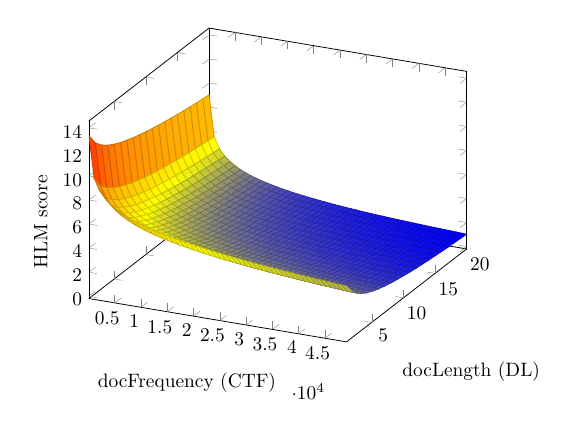
\begin{tikzpicture}[thick,scale=0.7, every node/.style={transform shape}] \begin{axis}[
 %title={},
 %y dir=reverse, 
 %x dir=reverse, 
 ylabel={docLength (DL)},
 xlabel={docFrequency (CTF)},
 zlabel={HLM score},
 max space between ticks=16pt
% yticklabels={0k,100k}
 ] 

		\addplot3[surf] coordinates { 
%patch,patch type=biquadratic, shader=faceted,patch refines=3

(100.00,20.00,9.02)(100.00,19.00,9.09)(100.00,18.00,9.17)(100.00,17.00,9.25)(100.00,16.00,9.34)(100.00,15.00,9.43)(100.00,14.00,9.53)(100.00,13.00,9.64)(100.00,12.00,9.75)(100.00,11.00,9.88)(100.00,10.00,10.02)(100.00,9.00,10.17)(100.00,8.00,10.34)(100.00,7.00,10.53)(100.00,6.00,10.75)(100.00,5.00,11.02)(100.00,4.00,11.34)(100.00,3.00,11.75)(100.00,2.00,12.34)(100.00,1.00,13.34)

(1100.00,20.00,5.59)(1100.00,19.00,5.66)(1100.00,18.00,5.73)(1100.00,17.00,5.82)(1100.00,16.00,5.90)(1100.00,15.00,5.99)(1100.00,14.00,6.09)(1100.00,13.00,6.20)(1100.00,12.00,6.31)(1100.00,11.00,6.43)(1100.00,10.00,6.57)(1100.00,9.00,6.72)(1100.00,8.00,6.89)(1100.00,7.00,7.08)(1100.00,6.00,7.30)(1100.00,5.00,7.56)(1100.00,4.00,7.88)(1100.00,3.00,8.30)(1100.00,2.00,8.88)(1100.00,1.00,9.88)

(2100.00,20.00,4.68)(2100.00,19.00,4.75)(2100.00,18.00,4.83)(2100.00,17.00,4.91)(2100.00,16.00,4.99)(2100.00,15.00,5.08)(2100.00,14.00,5.18)(2100.00,13.00,5.28)(2100.00,12.00,5.39)(2100.00,11.00,5.52)(2100.00,10.00,5.65)(2100.00,9.00,5.80)(2100.00,8.00,5.97)(2100.00,7.00,6.16)(2100.00,6.00,6.38)(2100.00,5.00,6.64)(2100.00,4.00,6.96)(2100.00,3.00,7.37)(2100.00,2.00,7.95)(2100.00,1.00,8.95)

(3100.00,20.00,4.14)(3100.00,19.00,4.21)(3100.00,18.00,4.29)(3100.00,17.00,4.37)(3100.00,16.00,4.45)(3100.00,15.00,4.54)(3100.00,14.00,4.63)(3100.00,13.00,4.74)(3100.00,12.00,4.85)(3100.00,11.00,4.97)(3100.00,10.00,5.10)(3100.00,9.00,5.25)(3100.00,8.00,5.42)(3100.00,7.00,5.60)(3100.00,6.00,5.82)(3100.00,5.00,6.08)(3100.00,4.00,6.40)(3100.00,3.00,6.81)(3100.00,2.00,7.39)(3100.00,1.00,8.39)

(4100.00,20.00,3.77)(4100.00,19.00,3.84)(4100.00,18.00,3.91)(4100.00,17.00,3.99)(4100.00,16.00,4.07)(4100.00,15.00,4.16)(4100.00,14.00,4.25)(4100.00,13.00,4.35)(4100.00,12.00,4.46)(4100.00,11.00,4.58)(4100.00,10.00,4.71)(4100.00,9.00,4.86)(4100.00,8.00,5.02)(4100.00,7.00,5.21)(4100.00,6.00,5.43)(4100.00,5.00,5.69)(4100.00,4.00,6.00)(4100.00,3.00,6.41)(4100.00,2.00,6.99)(4100.00,1.00,7.98)

(5100.00,20.00,3.48)(5100.00,19.00,3.55)(5100.00,18.00,3.62)(5100.00,17.00,3.69)(5100.00,16.00,3.77)(5100.00,15.00,3.86)(5100.00,14.00,3.95)(5100.00,13.00,4.05)(5100.00,12.00,4.16)(5100.00,11.00,4.28)(5100.00,10.00,4.41)(5100.00,9.00,4.56)(5100.00,8.00,4.72)(5100.00,7.00,4.91)(5100.00,6.00,5.12)(5100.00,5.00,5.38)(5100.00,4.00,5.69)(5100.00,3.00,6.10)(5100.00,2.00,6.68)(5100.00,1.00,7.67)

(6100.00,20.00,3.24)(6100.00,19.00,3.31)(6100.00,18.00,3.38)(6100.00,17.00,3.46)(6100.00,16.00,3.54)(6100.00,15.00,3.62)(6100.00,14.00,3.71)(6100.00,13.00,3.81)(6100.00,12.00,3.92)(6100.00,11.00,4.04)(6100.00,10.00,4.17)(6100.00,9.00,4.31)(6100.00,8.00,4.47)(6100.00,7.00,4.66)(6100.00,6.00,4.87)(6100.00,5.00,5.13)(6100.00,4.00,5.44)(6100.00,3.00,5.85)(6100.00,2.00,6.42)(6100.00,1.00,7.41)

(7100.00,20.00,3.05)(7100.00,19.00,3.12)(7100.00,18.00,3.18)(7100.00,17.00,3.26)(7100.00,16.00,3.34)(7100.00,15.00,3.42)(7100.00,14.00,3.51)(7100.00,13.00,3.61)(7100.00,12.00,3.72)(7100.00,11.00,3.83)(7100.00,10.00,3.96)(7100.00,9.00,4.10)(7100.00,8.00,4.26)(7100.00,7.00,4.45)(7100.00,6.00,4.66)(7100.00,5.00,4.91)(7100.00,4.00,5.23)(7100.00,3.00,5.63)(7100.00,2.00,6.21)(7100.00,1.00,7.20)

(8100.00,20.00,2.88)(8100.00,19.00,2.95)(8100.00,18.00,3.02)(8100.00,17.00,3.09)(8100.00,16.00,3.17)(8100.00,15.00,3.25)(8100.00,14.00,3.34)(8100.00,13.00,3.44)(8100.00,12.00,3.54)(8100.00,11.00,3.66)(8100.00,10.00,3.78)(8100.00,9.00,3.92)(8100.00,8.00,4.08)(8100.00,7.00,4.27)(8100.00,6.00,4.48)(8100.00,5.00,4.73)(8100.00,4.00,5.04)(8100.00,3.00,5.45)(8100.00,2.00,6.02)(8100.00,1.00,7.01)

(9100.00,20.00,2.74)(9100.00,19.00,2.80)(9100.00,18.00,2.87)(9100.00,17.00,2.94)(9100.00,16.00,3.02)(9100.00,15.00,3.10)(9100.00,14.00,3.19)(9100.00,13.00,3.28)(9100.00,12.00,3.39)(9100.00,11.00,3.50)(9100.00,10.00,3.63)(9100.00,9.00,3.77)(9100.00,8.00,3.93)(9100.00,7.00,4.11)(9100.00,6.00,4.32)(9100.00,5.00,4.57)(9100.00,4.00,4.88)(9100.00,3.00,5.28)(9100.00,2.00,5.85)(9100.00,1.00,6.84)

(10100.00,20.00,2.61)(10100.00,19.00,2.68)(10100.00,18.00,2.74)(10100.00,17.00,2.81)(10100.00,16.00,2.89)(10100.00,15.00,2.97)(10100.00,14.00,3.06)(10100.00,13.00,3.15)(10100.00,12.00,3.25)(10100.00,11.00,3.37)(10100.00,10.00,3.49)(10100.00,9.00,3.63)(10100.00,8.00,3.79)(10100.00,7.00,3.97)(10100.00,6.00,4.18)(10100.00,5.00,4.43)(10100.00,4.00,4.73)(10100.00,3.00,5.13)(10100.00,2.00,5.71)(10100.00,1.00,6.69)

(11100.00,20.00,2.50)(11100.00,19.00,2.56)(11100.00,18.00,2.63)(11100.00,17.00,2.70)(11100.00,16.00,2.77)(11100.00,15.00,2.85)(11100.00,14.00,2.94)(11100.00,13.00,3.03)(11100.00,12.00,3.13)(11100.00,11.00,3.24)(11100.00,10.00,3.37)(11100.00,9.00,3.51)(11100.00,8.00,3.66)(11100.00,7.00,3.84)(11100.00,6.00,4.05)(11100.00,5.00,4.30)(11100.00,4.00,4.60)(11100.00,3.00,5.00)(11100.00,2.00,5.57)(11100.00,1.00,6.56)

(12100.00,20.00,2.40)(12100.00,19.00,2.46)(12100.00,18.00,2.52)(12100.00,17.00,2.59)(12100.00,16.00,2.67)(12100.00,15.00,2.74)(12100.00,14.00,2.83)(12100.00,13.00,2.92)(12100.00,12.00,3.02)(12100.00,11.00,3.13)(12100.00,10.00,3.26)(12100.00,9.00,3.39)(12100.00,8.00,3.55)(12100.00,7.00,3.72)(12100.00,6.00,3.93)(12100.00,5.00,4.18)(12100.00,4.00,4.48)(12100.00,3.00,4.88)(12100.00,2.00,5.45)(12100.00,1.00,6.43)

(13100.00,20.00,2.31)(13100.00,19.00,2.37)(13100.00,18.00,2.43)(13100.00,17.00,2.50)(13100.00,16.00,2.57)(13100.00,15.00,2.65)(13100.00,14.00,2.73)(13100.00,13.00,2.82)(13100.00,12.00,2.92)(13100.00,11.00,3.03)(13100.00,10.00,3.15)(13100.00,9.00,3.29)(13100.00,8.00,3.44)(13100.00,7.00,3.62)(13100.00,6.00,3.82)(13100.00,5.00,4.07)(13100.00,4.00,4.37)(13100.00,3.00,4.77)(13100.00,2.00,5.34)(13100.00,1.00,6.32)

(14100.00,20.00,2.22)(14100.00,19.00,2.28)(14100.00,18.00,2.34)(14100.00,17.00,2.41)(14100.00,16.00,2.48)(14100.00,15.00,2.56)(14100.00,14.00,2.64)(14100.00,13.00,2.73)(14100.00,12.00,2.83)(14100.00,11.00,2.94)(14100.00,10.00,3.06)(14100.00,9.00,3.19)(14100.00,8.00,3.35)(14100.00,7.00,3.52)(14100.00,6.00,3.73)(14100.00,5.00,3.97)(14100.00,4.00,4.27)(14100.00,3.00,4.67)(14100.00,2.00,5.24)(14100.00,1.00,6.22)

(15100.00,20.00,2.15)(15100.00,19.00,2.20)(15100.00,18.00,2.26)(15100.00,17.00,2.33)(15100.00,16.00,2.40)(15100.00,15.00,2.48)(15100.00,14.00,2.56)(15100.00,13.00,2.65)(15100.00,12.00,2.75)(15100.00,11.00,2.85)(15100.00,10.00,2.97)(15100.00,9.00,3.11)(15100.00,8.00,3.26)(15100.00,7.00,3.43)(15100.00,6.00,3.63)(15100.00,5.00,3.88)(15100.00,4.00,4.18)(15100.00,3.00,4.57)(15100.00,2.00,5.14)(15100.00,1.00,6.12)

(16100.00,20.00,2.07)(16100.00,19.00,2.13)(16100.00,18.00,2.19)(16100.00,17.00,2.26)(16100.00,16.00,2.33)(16100.00,15.00,2.40)(16100.00,14.00,2.48)(16100.00,13.00,2.57)(16100.00,12.00,2.67)(16100.00,11.00,2.77)(16100.00,10.00,2.89)(16100.00,9.00,3.02)(16100.00,8.00,3.17)(16100.00,7.00,3.35)(16100.00,6.00,3.55)(16100.00,5.00,3.79)(16100.00,4.00,4.09)(16100.00,3.00,4.49)(16100.00,2.00,5.05)(16100.00,1.00,6.03)

(17100.00,20.00,2.01)(17100.00,19.00,2.06)(17100.00,18.00,2.12)(17100.00,17.00,2.19)(17100.00,16.00,2.26)(17100.00,15.00,2.33)(17100.00,14.00,2.41)(17100.00,13.00,2.50)(17100.00,12.00,2.59)(17100.00,11.00,2.70)(17100.00,10.00,2.82)(17100.00,9.00,2.95)(17100.00,8.00,3.10)(17100.00,7.00,3.27)(17100.00,6.00,3.47)(17100.00,5.00,3.71)(17100.00,4.00,4.01)(17100.00,3.00,4.40)(17100.00,2.00,4.97)(17100.00,1.00,5.94)

(18100.00,20.00,1.95)(18100.00,19.00,2.00)(18100.00,18.00,2.06)(18100.00,17.00,2.12)(18100.00,16.00,2.19)(18100.00,15.00,2.27)(18100.00,14.00,2.35)(18100.00,13.00,2.43)(18100.00,12.00,2.53)(18100.00,11.00,2.63)(18100.00,10.00,2.75)(18100.00,9.00,2.88)(18100.00,8.00,3.03)(18100.00,7.00,3.20)(18100.00,6.00,3.40)(18100.00,5.00,3.64)(18100.00,4.00,3.93)(18100.00,3.00,4.33)(18100.00,2.00,4.89)(18100.00,1.00,5.86)

(19100.00,20.00,1.89)(19100.00,19.00,1.94)(19100.00,18.00,2.00)(19100.00,17.00,2.07)(19100.00,16.00,2.13)(19100.00,15.00,2.20)(19100.00,14.00,2.28)(19100.00,13.00,2.37)(19100.00,12.00,2.46)(19100.00,11.00,2.57)(19100.00,10.00,2.68)(19100.00,9.00,2.81)(19100.00,8.00,2.96)(19100.00,7.00,3.13)(19100.00,6.00,3.33)(19100.00,5.00,3.56)(19100.00,4.00,3.86)(19100.00,3.00,4.25)(19100.00,2.00,4.81)(19100.00,1.00,5.79)

(20100.00,20.00,1.84)(20100.00,19.00,1.89)(20100.00,18.00,1.95)(20100.00,17.00,2.01)(20100.00,16.00,2.08)(20100.00,15.00,2.15)(20100.00,14.00,2.23)(20100.00,13.00,2.31)(20100.00,12.00,2.40)(20100.00,11.00,2.51)(20100.00,10.00,2.62)(20100.00,9.00,2.75)(20100.00,8.00,2.89)(20100.00,7.00,3.06)(20100.00,6.00,3.26)(20100.00,5.00,3.50)(20100.00,4.00,3.79)(20100.00,3.00,4.18)(20100.00,2.00,4.74)(20100.00,1.00,5.71)

(21100.00,20.00,1.79)(21100.00,19.00,1.84)(21100.00,18.00,1.90)(21100.00,17.00,1.96)(21100.00,16.00,2.02)(21100.00,15.00,2.09)(21100.00,14.00,2.17)(21100.00,13.00,2.25)(21100.00,12.00,2.35)(21100.00,11.00,2.45)(21100.00,10.00,2.56)(21100.00,9.00,2.69)(21100.00,8.00,2.83)(21100.00,7.00,3.00)(21100.00,6.00,3.20)(21100.00,5.00,3.43)(21100.00,4.00,3.73)(21100.00,3.00,4.12)(21100.00,2.00,4.67)(21100.00,1.00,5.64)

(22100.00,20.00,1.74)(22100.00,19.00,1.79)(22100.00,18.00,1.85)(22100.00,17.00,1.91)(22100.00,16.00,1.97)(22100.00,15.00,2.04)(22100.00,14.00,2.12)(22100.00,13.00,2.20)(22100.00,12.00,2.29)(22100.00,11.00,2.39)(22100.00,10.00,2.51)(22100.00,9.00,2.63)(22100.00,8.00,2.78)(22100.00,7.00,2.94)(22100.00,6.00,3.14)(22100.00,5.00,3.37)(22100.00,4.00,3.67)(22100.00,3.00,4.05)(22100.00,2.00,4.61)(22100.00,1.00,5.58)

(23100.00,20.00,1.70)(23100.00,19.00,1.75)(23100.00,18.00,1.80)(23100.00,17.00,1.86)(23100.00,16.00,1.93)(23100.00,15.00,1.99)(23100.00,14.00,2.07)(23100.00,13.00,2.15)(23100.00,12.00,2.24)(23100.00,11.00,2.34)(23100.00,10.00,2.45)(23100.00,9.00,2.58)(23100.00,8.00,2.72)(23100.00,7.00,2.89)(23100.00,6.00,3.08)(23100.00,5.00,3.32)(23100.00,4.00,3.61)(23100.00,3.00,3.99)(23100.00,2.00,4.55)(23100.00,1.00,5.52)

(24100.00,20.00,1.65)(24100.00,19.00,1.70)(24100.00,18.00,1.76)(24100.00,17.00,1.82)(24100.00,16.00,1.88)(24100.00,15.00,1.95)(24100.00,14.00,2.02)(24100.00,13.00,2.10)(24100.00,12.00,2.19)(24100.00,11.00,2.29)(24100.00,10.00,2.40)(24100.00,9.00,2.53)(24100.00,8.00,2.67)(24100.00,7.00,2.83)(24100.00,6.00,3.03)(24100.00,5.00,3.26)(24100.00,4.00,3.55)(24100.00,3.00,3.94)(24100.00,2.00,4.49)(24100.00,1.00,5.46)

(25100.00,20.00,1.61)(25100.00,19.00,1.66)(25100.00,18.00,1.72)(25100.00,17.00,1.78)(25100.00,16.00,1.84)(25100.00,15.00,1.91)(25100.00,14.00,1.98)(25100.00,13.00,2.06)(25100.00,12.00,2.15)(25100.00,11.00,2.25)(25100.00,10.00,2.36)(25100.00,9.00,2.48)(25100.00,8.00,2.62)(25100.00,7.00,2.78)(25100.00,6.00,2.98)(25100.00,5.00,3.21)(25100.00,4.00,3.50)(25100.00,3.00,3.88)(25100.00,2.00,4.43)(25100.00,1.00,5.40)

(26100.00,20.00,1.58)(26100.00,19.00,1.63)(26100.00,18.00,1.68)(26100.00,17.00,1.74)(26100.00,16.00,1.80)(26100.00,15.00,1.86)(26100.00,14.00,1.94)(26100.00,13.00,2.02)(26100.00,12.00,2.11)(26100.00,11.00,2.20)(26100.00,10.00,2.31)(26100.00,9.00,2.43)(26100.00,8.00,2.57)(26100.00,7.00,2.74)(26100.00,6.00,2.93)(26100.00,5.00,3.16)(26100.00,4.00,3.45)(26100.00,3.00,3.83)(26100.00,2.00,4.38)(26100.00,1.00,5.34)

(27100.00,20.00,1.54)(27100.00,19.00,1.59)(27100.00,18.00,1.64)(27100.00,17.00,1.70)(27100.00,16.00,1.76)(27100.00,15.00,1.83)(27100.00,14.00,1.90)(27100.00,13.00,1.98)(27100.00,12.00,2.06)(27100.00,11.00,2.16)(27100.00,10.00,2.27)(27100.00,9.00,2.39)(27100.00,8.00,2.53)(27100.00,7.00,2.69)(27100.00,6.00,2.88)(27100.00,5.00,3.11)(27100.00,4.00,3.40)(27100.00,3.00,3.78)(27100.00,2.00,4.33)(27100.00,1.00,5.29)

(28100.00,20.00,1.51)(28100.00,19.00,1.55)(28100.00,18.00,1.61)(28100.00,17.00,1.66)(28100.00,16.00,1.72)(28100.00,15.00,1.79)(28100.00,14.00,1.86)(28100.00,13.00,1.94)(28100.00,12.00,2.02)(28100.00,11.00,2.12)(28100.00,10.00,2.23)(28100.00,9.00,2.35)(28100.00,8.00,2.49)(28100.00,7.00,2.65)(28100.00,6.00,2.83)(28100.00,5.00,3.06)(28100.00,4.00,3.35)(28100.00,3.00,3.73)(28100.00,2.00,4.28)(28100.00,1.00,5.24)

(29100.00,20.00,1.47)(29100.00,19.00,1.52)(29100.00,18.00,1.57)(29100.00,17.00,1.63)(29100.00,16.00,1.69)(29100.00,15.00,1.75)(29100.00,14.00,1.82)(29100.00,13.00,1.90)(29100.00,12.00,1.99)(29100.00,11.00,2.08)(29100.00,10.00,2.19)(29100.00,9.00,2.31)(29100.00,8.00,2.44)(29100.00,7.00,2.60)(29100.00,6.00,2.79)(29100.00,5.00,3.02)(29100.00,4.00,3.31)(29100.00,3.00,3.68)(29100.00,2.00,4.23)(29100.00,1.00,5.19)

(30100.00,20.00,1.44)(30100.00,19.00,1.49)(30100.00,18.00,1.54)(30100.00,17.00,1.60)(30100.00,16.00,1.65)(30100.00,15.00,1.72)(30100.00,14.00,1.79)(30100.00,13.00,1.87)(30100.00,12.00,1.95)(30100.00,11.00,2.04)(30100.00,10.00,2.15)(30100.00,9.00,2.27)(30100.00,8.00,2.40)(30100.00,7.00,2.56)(30100.00,6.00,2.75)(30100.00,5.00,2.98)(30100.00,4.00,3.26)(30100.00,3.00,3.64)(30100.00,2.00,4.18)(30100.00,1.00,5.14)

(31100.00,20.00,1.41)(31100.00,19.00,1.46)(31100.00,18.00,1.51)(31100.00,17.00,1.56)(31100.00,16.00,1.62)(31100.00,15.00,1.69)(31100.00,14.00,1.76)(31100.00,13.00,1.83)(31100.00,12.00,1.92)(31100.00,11.00,2.01)(31100.00,10.00,2.11)(31100.00,9.00,2.23)(31100.00,8.00,2.37)(31100.00,7.00,2.52)(31100.00,6.00,2.71)(31100.00,5.00,2.94)(31100.00,4.00,3.22)(31100.00,3.00,3.60)(31100.00,2.00,4.14)(31100.00,1.00,5.10)

(32100.00,20.00,1.38)(32100.00,19.00,1.43)(32100.00,18.00,1.48)(32100.00,17.00,1.53)(32100.00,16.00,1.59)(32100.00,15.00,1.65)(32100.00,14.00,1.72)(32100.00,13.00,1.80)(32100.00,12.00,1.88)(32100.00,11.00,1.97)(32100.00,10.00,2.08)(32100.00,9.00,2.20)(32100.00,8.00,2.33)(32100.00,7.00,2.49)(32100.00,6.00,2.67)(32100.00,5.00,2.90)(32100.00,4.00,3.18)(32100.00,3.00,3.55)(32100.00,2.00,4.10)(32100.00,1.00,5.05)

(33100.00,20.00,1.36)(33100.00,19.00,1.40)(33100.00,18.00,1.45)(33100.00,17.00,1.50)(33100.00,16.00,1.56)(33100.00,15.00,1.62)(33100.00,14.00,1.69)(33100.00,13.00,1.77)(33100.00,12.00,1.85)(33100.00,11.00,1.94)(33100.00,10.00,2.04)(33100.00,9.00,2.16)(33100.00,8.00,2.29)(33100.00,7.00,2.45)(33100.00,6.00,2.63)(33100.00,5.00,2.86)(33100.00,4.00,3.14)(33100.00,3.00,3.51)(33100.00,2.00,4.06)(33100.00,1.00,5.01)

(34100.00,20.00,1.33)(34100.00,19.00,1.38)(34100.00,18.00,1.42)(34100.00,17.00,1.48)(34100.00,16.00,1.53)(34100.00,15.00,1.60)(34100.00,14.00,1.66)(34100.00,13.00,1.74)(34100.00,12.00,1.82)(34100.00,11.00,1.91)(34100.00,10.00,2.01)(34100.00,9.00,2.13)(34100.00,8.00,2.26)(34100.00,7.00,2.41)(34100.00,6.00,2.60)(34100.00,5.00,2.82)(34100.00,4.00,3.10)(34100.00,3.00,3.47)(34100.00,2.00,4.01)(34100.00,1.00,4.97)

(35100.00,20.00,1.31)(35100.00,19.00,1.35)(35100.00,18.00,1.40)(35100.00,17.00,1.45)(35100.00,16.00,1.51)(35100.00,15.00,1.57)(35100.00,14.00,1.63)(35100.00,13.00,1.71)(35100.00,12.00,1.79)(35100.00,11.00,1.88)(35100.00,10.00,1.98)(35100.00,9.00,2.10)(35100.00,8.00,2.23)(35100.00,7.00,2.38)(35100.00,6.00,2.56)(35100.00,5.00,2.79)(35100.00,4.00,3.06)(35100.00,3.00,3.44)(35100.00,2.00,3.98)(35100.00,1.00,4.93)

(36100.00,20.00,1.28)(36100.00,19.00,1.33)(36100.00,18.00,1.37)(36100.00,17.00,1.43)(36100.00,16.00,1.48)(36100.00,15.00,1.54)(36100.00,14.00,1.61)(36100.00,13.00,1.68)(36100.00,12.00,1.76)(36100.00,11.00,1.85)(36100.00,10.00,1.95)(36100.00,9.00,2.06)(36100.00,8.00,2.20)(36100.00,7.00,2.35)(36100.00,6.00,2.53)(36100.00,5.00,2.75)(36100.00,4.00,3.03)(36100.00,3.00,3.40)(36100.00,2.00,3.94)(36100.00,1.00,4.89)

(37100.00,20.00,1.26)(37100.00,19.00,1.30)(37100.00,18.00,1.35)(37100.00,17.00,1.40)(37100.00,16.00,1.46)(37100.00,15.00,1.52)(37100.00,14.00,1.58)(37100.00,13.00,1.65)(37100.00,12.00,1.73)(37100.00,11.00,1.82)(37100.00,10.00,1.92)(37100.00,9.00,2.03)(37100.00,8.00,2.17)(37100.00,7.00,2.32)(37100.00,6.00,2.50)(37100.00,5.00,2.72)(37100.00,4.00,2.99)(37100.00,3.00,3.36)(37100.00,2.00,3.90)(37100.00,1.00,4.85)

(38100.00,20.00,1.24)(38100.00,19.00,1.28)(38100.00,18.00,1.33)(38100.00,17.00,1.38)(38100.00,16.00,1.43)(38100.00,15.00,1.49)(38100.00,14.00,1.56)(38100.00,13.00,1.63)(38100.00,12.00,1.71)(38100.00,11.00,1.79)(38100.00,10.00,1.89)(38100.00,9.00,2.01)(38100.00,8.00,2.14)(38100.00,7.00,2.29)(38100.00,6.00,2.47)(38100.00,5.00,2.68)(38100.00,4.00,2.96)(38100.00,3.00,3.33)(38100.00,2.00,3.87)(38100.00,1.00,4.81)

(39100.00,20.00,1.22)(39100.00,19.00,1.26)(39100.00,18.00,1.30)(39100.00,17.00,1.35)(39100.00,16.00,1.41)(39100.00,15.00,1.47)(39100.00,14.00,1.53)(39100.00,13.00,1.60)(39100.00,12.00,1.68)(39100.00,11.00,1.77)(39100.00,10.00,1.87)(39100.00,9.00,1.98)(39100.00,8.00,2.11)(39100.00,7.00,2.26)(39100.00,6.00,2.44)(39100.00,5.00,2.65)(39100.00,4.00,2.93)(39100.00,3.00,3.30)(39100.00,2.00,3.83)(39100.00,1.00,4.78)

(40100.00,20.00,1.20)(40100.00,19.00,1.24)(40100.00,18.00,1.28)(40100.00,17.00,1.33)(40100.00,16.00,1.39)(40100.00,15.00,1.44)(40100.00,14.00,1.51)(40100.00,13.00,1.58)(40100.00,12.00,1.66)(40100.00,11.00,1.74)(40100.00,10.00,1.84)(40100.00,9.00,1.95)(40100.00,8.00,2.08)(40100.00,7.00,2.23)(40100.00,6.00,2.41)(40100.00,5.00,2.62)(40100.00,4.00,2.90)(40100.00,3.00,3.26)(40100.00,2.00,3.80)(40100.00,1.00,4.74)

(41100.00,20.00,1.18)(41100.00,19.00,1.22)(41100.00,18.00,1.26)(41100.00,17.00,1.31)(41100.00,16.00,1.36)(41100.00,15.00,1.42)(41100.00,14.00,1.48)(41100.00,13.00,1.55)(41100.00,12.00,1.63)(41100.00,11.00,1.72)(41100.00,10.00,1.81)(41100.00,9.00,1.92)(41100.00,8.00,2.05)(41100.00,7.00,2.20)(41100.00,6.00,2.38)(41100.00,5.00,2.59)(41100.00,4.00,2.87)(41100.00,3.00,3.23)(41100.00,2.00,3.76)(41100.00,1.00,4.71)

(42100.00,20.00,1.16)(42100.00,19.00,1.20)(42100.00,18.00,1.24)(42100.00,17.00,1.29)(42100.00,16.00,1.34)(42100.00,15.00,1.40)(42100.00,14.00,1.46)(42100.00,13.00,1.53)(42100.00,12.00,1.61)(42100.00,11.00,1.69)(42100.00,10.00,1.79)(42100.00,9.00,1.90)(42100.00,8.00,2.03)(42100.00,7.00,2.17)(42100.00,6.00,2.35)(42100.00,5.00,2.56)(42100.00,4.00,2.84)(42100.00,3.00,3.20)(42100.00,2.00,3.73)(42100.00,1.00,4.68)

(43100.00,20.00,1.14)(43100.00,19.00,1.18)(43100.00,18.00,1.22)(43100.00,17.00,1.27)(43100.00,16.00,1.32)(43100.00,15.00,1.38)(43100.00,14.00,1.44)(43100.00,13.00,1.51)(43100.00,12.00,1.58)(43100.00,11.00,1.67)(43100.00,10.00,1.77)(43100.00,9.00,1.87)(43100.00,8.00,2.00)(43100.00,7.00,2.15)(43100.00,6.00,2.32)(43100.00,5.00,2.54)(43100.00,4.00,2.81)(43100.00,3.00,3.17)(43100.00,2.00,3.70)(43100.00,1.00,4.64)

(44100.00,20.00,1.12)(44100.00,19.00,1.16)(44100.00,18.00,1.20)(44100.00,17.00,1.25)(44100.00,16.00,1.30)(44100.00,15.00,1.36)(44100.00,14.00,1.42)(44100.00,13.00,1.49)(44100.00,12.00,1.56)(44100.00,11.00,1.65)(44100.00,10.00,1.74)(44100.00,9.00,1.85)(44100.00,8.00,1.98)(44100.00,7.00,2.12)(44100.00,6.00,2.30)(44100.00,5.00,2.51)(44100.00,4.00,2.78)(44100.00,3.00,3.14)(44100.00,2.00,3.67)(44100.00,1.00,4.61)

(45100.00,20.00,1.10)(45100.00,19.00,1.14)(45100.00,18.00,1.19)(45100.00,17.00,1.23)(45100.00,16.00,1.28)(45100.00,15.00,1.34)(45100.00,14.00,1.40)(45100.00,13.00,1.47)(45100.00,12.00,1.54)(45100.00,11.00,1.63)(45100.00,10.00,1.72)(45100.00,9.00,1.83)(45100.00,8.00,1.95)(45100.00,7.00,2.10)(45100.00,6.00,2.27)(45100.00,5.00,2.48)(45100.00,4.00,2.75)(45100.00,3.00,3.11)(45100.00,2.00,3.64)(45100.00,1.00,4.58)

(46100.00,20.00,1.09)(46100.00,19.00,1.12)(46100.00,18.00,1.17)(46100.00,17.00,1.21)(46100.00,16.00,1.26)(46100.00,15.00,1.32)(46100.00,14.00,1.38)(46100.00,13.00,1.45)(46100.00,12.00,1.52)(46100.00,11.00,1.60)(46100.00,10.00,1.70)(46100.00,9.00,1.80)(46100.00,8.00,1.93)(46100.00,7.00,2.07)(46100.00,6.00,2.24)(46100.00,5.00,2.46)(46100.00,4.00,2.72)(46100.00,3.00,3.08)(46100.00,2.00,3.61)(46100.00,1.00,4.55)

(47100.00,20.00,1.07)(47100.00,19.00,1.11)(47100.00,18.00,1.15)(47100.00,17.00,1.20)(47100.00,16.00,1.25)(47100.00,15.00,1.30)(47100.00,14.00,1.36)(47100.00,13.00,1.43)(47100.00,12.00,1.50)(47100.00,11.00,1.58)(47100.00,10.00,1.68)(47100.00,9.00,1.78)(47100.00,8.00,1.90)(47100.00,7.00,2.05)(47100.00,6.00,2.22)(47100.00,5.00,2.43)(47100.00,4.00,2.70)(47100.00,3.00,3.06)(47100.00,2.00,3.58)(47100.00,1.00,4.52)

(48100.00,20.00,1.05)(48100.00,19.00,1.09)(48100.00,18.00,1.13)(48100.00,17.00,1.18)(48100.00,16.00,1.23)(48100.00,15.00,1.28)(48100.00,14.00,1.34)(48100.00,13.00,1.41)(48100.00,12.00,1.48)(48100.00,11.00,1.56)(48100.00,10.00,1.66)(48100.00,9.00,1.76)(48100.00,8.00,1.88)(48100.00,7.00,2.03)(48100.00,6.00,2.20)(48100.00,5.00,2.41)(48100.00,4.00,2.67)(48100.00,3.00,3.03)(48100.00,2.00,3.55)(48100.00,1.00,4.49)

(49100.00,20.00,1.04)(49100.00,19.00,1.08)(49100.00,18.00,1.12)(49100.00,17.00,1.16)(49100.00,16.00,1.21)(49100.00,15.00,1.27)(49100.00,14.00,1.32)(49100.00,13.00,1.39)(49100.00,12.00,1.46)(49100.00,11.00,1.54)(49100.00,10.00,1.64)(49100.00,9.00,1.74)(49100.00,8.00,1.86)(49100.00,7.00,2.00)(49100.00,6.00,2.17)(49100.00,5.00,2.38)(49100.00,4.00,2.65)(49100.00,3.00,3.00)(49100.00,2.00,3.53)(49100.00,1.00,4.46)


}; \end{axis} \end{tikzpicture}

%		\label{hlm-ctf-dl}
%      \end{subfigure} 
%    \caption{HLM analysis}
%		\label{hlmanalysis}
%\end{figure}

%\begin{figure}[]
%	\centering
%	\caption{HLM: Doc. Frequency (CTF) vs, Doc. Length (DL)}
%	
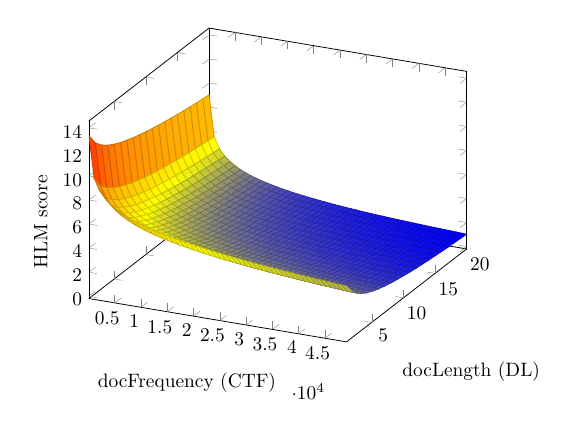
\begin{tikzpicture}[thick,scale=0.7, every node/.style={transform shape}] \begin{axis}[
 %title={},
 %y dir=reverse, 
 %x dir=reverse, 
 ylabel={docLength (DL)},
 xlabel={docFrequency (CTF)},
 zlabel={HLM score},
 max space between ticks=16pt
% yticklabels={0k,100k}
 ] 

		\addplot3[surf] coordinates { 
%patch,patch type=biquadratic, shader=faceted,patch refines=3

(100.00,20.00,9.02)(100.00,19.00,9.09)(100.00,18.00,9.17)(100.00,17.00,9.25)(100.00,16.00,9.34)(100.00,15.00,9.43)(100.00,14.00,9.53)(100.00,13.00,9.64)(100.00,12.00,9.75)(100.00,11.00,9.88)(100.00,10.00,10.02)(100.00,9.00,10.17)(100.00,8.00,10.34)(100.00,7.00,10.53)(100.00,6.00,10.75)(100.00,5.00,11.02)(100.00,4.00,11.34)(100.00,3.00,11.75)(100.00,2.00,12.34)(100.00,1.00,13.34)

(1100.00,20.00,5.59)(1100.00,19.00,5.66)(1100.00,18.00,5.73)(1100.00,17.00,5.82)(1100.00,16.00,5.90)(1100.00,15.00,5.99)(1100.00,14.00,6.09)(1100.00,13.00,6.20)(1100.00,12.00,6.31)(1100.00,11.00,6.43)(1100.00,10.00,6.57)(1100.00,9.00,6.72)(1100.00,8.00,6.89)(1100.00,7.00,7.08)(1100.00,6.00,7.30)(1100.00,5.00,7.56)(1100.00,4.00,7.88)(1100.00,3.00,8.30)(1100.00,2.00,8.88)(1100.00,1.00,9.88)

(2100.00,20.00,4.68)(2100.00,19.00,4.75)(2100.00,18.00,4.83)(2100.00,17.00,4.91)(2100.00,16.00,4.99)(2100.00,15.00,5.08)(2100.00,14.00,5.18)(2100.00,13.00,5.28)(2100.00,12.00,5.39)(2100.00,11.00,5.52)(2100.00,10.00,5.65)(2100.00,9.00,5.80)(2100.00,8.00,5.97)(2100.00,7.00,6.16)(2100.00,6.00,6.38)(2100.00,5.00,6.64)(2100.00,4.00,6.96)(2100.00,3.00,7.37)(2100.00,2.00,7.95)(2100.00,1.00,8.95)

(3100.00,20.00,4.14)(3100.00,19.00,4.21)(3100.00,18.00,4.29)(3100.00,17.00,4.37)(3100.00,16.00,4.45)(3100.00,15.00,4.54)(3100.00,14.00,4.63)(3100.00,13.00,4.74)(3100.00,12.00,4.85)(3100.00,11.00,4.97)(3100.00,10.00,5.10)(3100.00,9.00,5.25)(3100.00,8.00,5.42)(3100.00,7.00,5.60)(3100.00,6.00,5.82)(3100.00,5.00,6.08)(3100.00,4.00,6.40)(3100.00,3.00,6.81)(3100.00,2.00,7.39)(3100.00,1.00,8.39)

(4100.00,20.00,3.77)(4100.00,19.00,3.84)(4100.00,18.00,3.91)(4100.00,17.00,3.99)(4100.00,16.00,4.07)(4100.00,15.00,4.16)(4100.00,14.00,4.25)(4100.00,13.00,4.35)(4100.00,12.00,4.46)(4100.00,11.00,4.58)(4100.00,10.00,4.71)(4100.00,9.00,4.86)(4100.00,8.00,5.02)(4100.00,7.00,5.21)(4100.00,6.00,5.43)(4100.00,5.00,5.69)(4100.00,4.00,6.00)(4100.00,3.00,6.41)(4100.00,2.00,6.99)(4100.00,1.00,7.98)

(5100.00,20.00,3.48)(5100.00,19.00,3.55)(5100.00,18.00,3.62)(5100.00,17.00,3.69)(5100.00,16.00,3.77)(5100.00,15.00,3.86)(5100.00,14.00,3.95)(5100.00,13.00,4.05)(5100.00,12.00,4.16)(5100.00,11.00,4.28)(5100.00,10.00,4.41)(5100.00,9.00,4.56)(5100.00,8.00,4.72)(5100.00,7.00,4.91)(5100.00,6.00,5.12)(5100.00,5.00,5.38)(5100.00,4.00,5.69)(5100.00,3.00,6.10)(5100.00,2.00,6.68)(5100.00,1.00,7.67)

(6100.00,20.00,3.24)(6100.00,19.00,3.31)(6100.00,18.00,3.38)(6100.00,17.00,3.46)(6100.00,16.00,3.54)(6100.00,15.00,3.62)(6100.00,14.00,3.71)(6100.00,13.00,3.81)(6100.00,12.00,3.92)(6100.00,11.00,4.04)(6100.00,10.00,4.17)(6100.00,9.00,4.31)(6100.00,8.00,4.47)(6100.00,7.00,4.66)(6100.00,6.00,4.87)(6100.00,5.00,5.13)(6100.00,4.00,5.44)(6100.00,3.00,5.85)(6100.00,2.00,6.42)(6100.00,1.00,7.41)

(7100.00,20.00,3.05)(7100.00,19.00,3.12)(7100.00,18.00,3.18)(7100.00,17.00,3.26)(7100.00,16.00,3.34)(7100.00,15.00,3.42)(7100.00,14.00,3.51)(7100.00,13.00,3.61)(7100.00,12.00,3.72)(7100.00,11.00,3.83)(7100.00,10.00,3.96)(7100.00,9.00,4.10)(7100.00,8.00,4.26)(7100.00,7.00,4.45)(7100.00,6.00,4.66)(7100.00,5.00,4.91)(7100.00,4.00,5.23)(7100.00,3.00,5.63)(7100.00,2.00,6.21)(7100.00,1.00,7.20)

(8100.00,20.00,2.88)(8100.00,19.00,2.95)(8100.00,18.00,3.02)(8100.00,17.00,3.09)(8100.00,16.00,3.17)(8100.00,15.00,3.25)(8100.00,14.00,3.34)(8100.00,13.00,3.44)(8100.00,12.00,3.54)(8100.00,11.00,3.66)(8100.00,10.00,3.78)(8100.00,9.00,3.92)(8100.00,8.00,4.08)(8100.00,7.00,4.27)(8100.00,6.00,4.48)(8100.00,5.00,4.73)(8100.00,4.00,5.04)(8100.00,3.00,5.45)(8100.00,2.00,6.02)(8100.00,1.00,7.01)

(9100.00,20.00,2.74)(9100.00,19.00,2.80)(9100.00,18.00,2.87)(9100.00,17.00,2.94)(9100.00,16.00,3.02)(9100.00,15.00,3.10)(9100.00,14.00,3.19)(9100.00,13.00,3.28)(9100.00,12.00,3.39)(9100.00,11.00,3.50)(9100.00,10.00,3.63)(9100.00,9.00,3.77)(9100.00,8.00,3.93)(9100.00,7.00,4.11)(9100.00,6.00,4.32)(9100.00,5.00,4.57)(9100.00,4.00,4.88)(9100.00,3.00,5.28)(9100.00,2.00,5.85)(9100.00,1.00,6.84)

(10100.00,20.00,2.61)(10100.00,19.00,2.68)(10100.00,18.00,2.74)(10100.00,17.00,2.81)(10100.00,16.00,2.89)(10100.00,15.00,2.97)(10100.00,14.00,3.06)(10100.00,13.00,3.15)(10100.00,12.00,3.25)(10100.00,11.00,3.37)(10100.00,10.00,3.49)(10100.00,9.00,3.63)(10100.00,8.00,3.79)(10100.00,7.00,3.97)(10100.00,6.00,4.18)(10100.00,5.00,4.43)(10100.00,4.00,4.73)(10100.00,3.00,5.13)(10100.00,2.00,5.71)(10100.00,1.00,6.69)

(11100.00,20.00,2.50)(11100.00,19.00,2.56)(11100.00,18.00,2.63)(11100.00,17.00,2.70)(11100.00,16.00,2.77)(11100.00,15.00,2.85)(11100.00,14.00,2.94)(11100.00,13.00,3.03)(11100.00,12.00,3.13)(11100.00,11.00,3.24)(11100.00,10.00,3.37)(11100.00,9.00,3.51)(11100.00,8.00,3.66)(11100.00,7.00,3.84)(11100.00,6.00,4.05)(11100.00,5.00,4.30)(11100.00,4.00,4.60)(11100.00,3.00,5.00)(11100.00,2.00,5.57)(11100.00,1.00,6.56)

(12100.00,20.00,2.40)(12100.00,19.00,2.46)(12100.00,18.00,2.52)(12100.00,17.00,2.59)(12100.00,16.00,2.67)(12100.00,15.00,2.74)(12100.00,14.00,2.83)(12100.00,13.00,2.92)(12100.00,12.00,3.02)(12100.00,11.00,3.13)(12100.00,10.00,3.26)(12100.00,9.00,3.39)(12100.00,8.00,3.55)(12100.00,7.00,3.72)(12100.00,6.00,3.93)(12100.00,5.00,4.18)(12100.00,4.00,4.48)(12100.00,3.00,4.88)(12100.00,2.00,5.45)(12100.00,1.00,6.43)

(13100.00,20.00,2.31)(13100.00,19.00,2.37)(13100.00,18.00,2.43)(13100.00,17.00,2.50)(13100.00,16.00,2.57)(13100.00,15.00,2.65)(13100.00,14.00,2.73)(13100.00,13.00,2.82)(13100.00,12.00,2.92)(13100.00,11.00,3.03)(13100.00,10.00,3.15)(13100.00,9.00,3.29)(13100.00,8.00,3.44)(13100.00,7.00,3.62)(13100.00,6.00,3.82)(13100.00,5.00,4.07)(13100.00,4.00,4.37)(13100.00,3.00,4.77)(13100.00,2.00,5.34)(13100.00,1.00,6.32)

(14100.00,20.00,2.22)(14100.00,19.00,2.28)(14100.00,18.00,2.34)(14100.00,17.00,2.41)(14100.00,16.00,2.48)(14100.00,15.00,2.56)(14100.00,14.00,2.64)(14100.00,13.00,2.73)(14100.00,12.00,2.83)(14100.00,11.00,2.94)(14100.00,10.00,3.06)(14100.00,9.00,3.19)(14100.00,8.00,3.35)(14100.00,7.00,3.52)(14100.00,6.00,3.73)(14100.00,5.00,3.97)(14100.00,4.00,4.27)(14100.00,3.00,4.67)(14100.00,2.00,5.24)(14100.00,1.00,6.22)

(15100.00,20.00,2.15)(15100.00,19.00,2.20)(15100.00,18.00,2.26)(15100.00,17.00,2.33)(15100.00,16.00,2.40)(15100.00,15.00,2.48)(15100.00,14.00,2.56)(15100.00,13.00,2.65)(15100.00,12.00,2.75)(15100.00,11.00,2.85)(15100.00,10.00,2.97)(15100.00,9.00,3.11)(15100.00,8.00,3.26)(15100.00,7.00,3.43)(15100.00,6.00,3.63)(15100.00,5.00,3.88)(15100.00,4.00,4.18)(15100.00,3.00,4.57)(15100.00,2.00,5.14)(15100.00,1.00,6.12)

(16100.00,20.00,2.07)(16100.00,19.00,2.13)(16100.00,18.00,2.19)(16100.00,17.00,2.26)(16100.00,16.00,2.33)(16100.00,15.00,2.40)(16100.00,14.00,2.48)(16100.00,13.00,2.57)(16100.00,12.00,2.67)(16100.00,11.00,2.77)(16100.00,10.00,2.89)(16100.00,9.00,3.02)(16100.00,8.00,3.17)(16100.00,7.00,3.35)(16100.00,6.00,3.55)(16100.00,5.00,3.79)(16100.00,4.00,4.09)(16100.00,3.00,4.49)(16100.00,2.00,5.05)(16100.00,1.00,6.03)

(17100.00,20.00,2.01)(17100.00,19.00,2.06)(17100.00,18.00,2.12)(17100.00,17.00,2.19)(17100.00,16.00,2.26)(17100.00,15.00,2.33)(17100.00,14.00,2.41)(17100.00,13.00,2.50)(17100.00,12.00,2.59)(17100.00,11.00,2.70)(17100.00,10.00,2.82)(17100.00,9.00,2.95)(17100.00,8.00,3.10)(17100.00,7.00,3.27)(17100.00,6.00,3.47)(17100.00,5.00,3.71)(17100.00,4.00,4.01)(17100.00,3.00,4.40)(17100.00,2.00,4.97)(17100.00,1.00,5.94)

(18100.00,20.00,1.95)(18100.00,19.00,2.00)(18100.00,18.00,2.06)(18100.00,17.00,2.12)(18100.00,16.00,2.19)(18100.00,15.00,2.27)(18100.00,14.00,2.35)(18100.00,13.00,2.43)(18100.00,12.00,2.53)(18100.00,11.00,2.63)(18100.00,10.00,2.75)(18100.00,9.00,2.88)(18100.00,8.00,3.03)(18100.00,7.00,3.20)(18100.00,6.00,3.40)(18100.00,5.00,3.64)(18100.00,4.00,3.93)(18100.00,3.00,4.33)(18100.00,2.00,4.89)(18100.00,1.00,5.86)

(19100.00,20.00,1.89)(19100.00,19.00,1.94)(19100.00,18.00,2.00)(19100.00,17.00,2.07)(19100.00,16.00,2.13)(19100.00,15.00,2.20)(19100.00,14.00,2.28)(19100.00,13.00,2.37)(19100.00,12.00,2.46)(19100.00,11.00,2.57)(19100.00,10.00,2.68)(19100.00,9.00,2.81)(19100.00,8.00,2.96)(19100.00,7.00,3.13)(19100.00,6.00,3.33)(19100.00,5.00,3.56)(19100.00,4.00,3.86)(19100.00,3.00,4.25)(19100.00,2.00,4.81)(19100.00,1.00,5.79)

(20100.00,20.00,1.84)(20100.00,19.00,1.89)(20100.00,18.00,1.95)(20100.00,17.00,2.01)(20100.00,16.00,2.08)(20100.00,15.00,2.15)(20100.00,14.00,2.23)(20100.00,13.00,2.31)(20100.00,12.00,2.40)(20100.00,11.00,2.51)(20100.00,10.00,2.62)(20100.00,9.00,2.75)(20100.00,8.00,2.89)(20100.00,7.00,3.06)(20100.00,6.00,3.26)(20100.00,5.00,3.50)(20100.00,4.00,3.79)(20100.00,3.00,4.18)(20100.00,2.00,4.74)(20100.00,1.00,5.71)

(21100.00,20.00,1.79)(21100.00,19.00,1.84)(21100.00,18.00,1.90)(21100.00,17.00,1.96)(21100.00,16.00,2.02)(21100.00,15.00,2.09)(21100.00,14.00,2.17)(21100.00,13.00,2.25)(21100.00,12.00,2.35)(21100.00,11.00,2.45)(21100.00,10.00,2.56)(21100.00,9.00,2.69)(21100.00,8.00,2.83)(21100.00,7.00,3.00)(21100.00,6.00,3.20)(21100.00,5.00,3.43)(21100.00,4.00,3.73)(21100.00,3.00,4.12)(21100.00,2.00,4.67)(21100.00,1.00,5.64)

(22100.00,20.00,1.74)(22100.00,19.00,1.79)(22100.00,18.00,1.85)(22100.00,17.00,1.91)(22100.00,16.00,1.97)(22100.00,15.00,2.04)(22100.00,14.00,2.12)(22100.00,13.00,2.20)(22100.00,12.00,2.29)(22100.00,11.00,2.39)(22100.00,10.00,2.51)(22100.00,9.00,2.63)(22100.00,8.00,2.78)(22100.00,7.00,2.94)(22100.00,6.00,3.14)(22100.00,5.00,3.37)(22100.00,4.00,3.67)(22100.00,3.00,4.05)(22100.00,2.00,4.61)(22100.00,1.00,5.58)

(23100.00,20.00,1.70)(23100.00,19.00,1.75)(23100.00,18.00,1.80)(23100.00,17.00,1.86)(23100.00,16.00,1.93)(23100.00,15.00,1.99)(23100.00,14.00,2.07)(23100.00,13.00,2.15)(23100.00,12.00,2.24)(23100.00,11.00,2.34)(23100.00,10.00,2.45)(23100.00,9.00,2.58)(23100.00,8.00,2.72)(23100.00,7.00,2.89)(23100.00,6.00,3.08)(23100.00,5.00,3.32)(23100.00,4.00,3.61)(23100.00,3.00,3.99)(23100.00,2.00,4.55)(23100.00,1.00,5.52)

(24100.00,20.00,1.65)(24100.00,19.00,1.70)(24100.00,18.00,1.76)(24100.00,17.00,1.82)(24100.00,16.00,1.88)(24100.00,15.00,1.95)(24100.00,14.00,2.02)(24100.00,13.00,2.10)(24100.00,12.00,2.19)(24100.00,11.00,2.29)(24100.00,10.00,2.40)(24100.00,9.00,2.53)(24100.00,8.00,2.67)(24100.00,7.00,2.83)(24100.00,6.00,3.03)(24100.00,5.00,3.26)(24100.00,4.00,3.55)(24100.00,3.00,3.94)(24100.00,2.00,4.49)(24100.00,1.00,5.46)

(25100.00,20.00,1.61)(25100.00,19.00,1.66)(25100.00,18.00,1.72)(25100.00,17.00,1.78)(25100.00,16.00,1.84)(25100.00,15.00,1.91)(25100.00,14.00,1.98)(25100.00,13.00,2.06)(25100.00,12.00,2.15)(25100.00,11.00,2.25)(25100.00,10.00,2.36)(25100.00,9.00,2.48)(25100.00,8.00,2.62)(25100.00,7.00,2.78)(25100.00,6.00,2.98)(25100.00,5.00,3.21)(25100.00,4.00,3.50)(25100.00,3.00,3.88)(25100.00,2.00,4.43)(25100.00,1.00,5.40)

(26100.00,20.00,1.58)(26100.00,19.00,1.63)(26100.00,18.00,1.68)(26100.00,17.00,1.74)(26100.00,16.00,1.80)(26100.00,15.00,1.86)(26100.00,14.00,1.94)(26100.00,13.00,2.02)(26100.00,12.00,2.11)(26100.00,11.00,2.20)(26100.00,10.00,2.31)(26100.00,9.00,2.43)(26100.00,8.00,2.57)(26100.00,7.00,2.74)(26100.00,6.00,2.93)(26100.00,5.00,3.16)(26100.00,4.00,3.45)(26100.00,3.00,3.83)(26100.00,2.00,4.38)(26100.00,1.00,5.34)

(27100.00,20.00,1.54)(27100.00,19.00,1.59)(27100.00,18.00,1.64)(27100.00,17.00,1.70)(27100.00,16.00,1.76)(27100.00,15.00,1.83)(27100.00,14.00,1.90)(27100.00,13.00,1.98)(27100.00,12.00,2.06)(27100.00,11.00,2.16)(27100.00,10.00,2.27)(27100.00,9.00,2.39)(27100.00,8.00,2.53)(27100.00,7.00,2.69)(27100.00,6.00,2.88)(27100.00,5.00,3.11)(27100.00,4.00,3.40)(27100.00,3.00,3.78)(27100.00,2.00,4.33)(27100.00,1.00,5.29)

(28100.00,20.00,1.51)(28100.00,19.00,1.55)(28100.00,18.00,1.61)(28100.00,17.00,1.66)(28100.00,16.00,1.72)(28100.00,15.00,1.79)(28100.00,14.00,1.86)(28100.00,13.00,1.94)(28100.00,12.00,2.02)(28100.00,11.00,2.12)(28100.00,10.00,2.23)(28100.00,9.00,2.35)(28100.00,8.00,2.49)(28100.00,7.00,2.65)(28100.00,6.00,2.83)(28100.00,5.00,3.06)(28100.00,4.00,3.35)(28100.00,3.00,3.73)(28100.00,2.00,4.28)(28100.00,1.00,5.24)

(29100.00,20.00,1.47)(29100.00,19.00,1.52)(29100.00,18.00,1.57)(29100.00,17.00,1.63)(29100.00,16.00,1.69)(29100.00,15.00,1.75)(29100.00,14.00,1.82)(29100.00,13.00,1.90)(29100.00,12.00,1.99)(29100.00,11.00,2.08)(29100.00,10.00,2.19)(29100.00,9.00,2.31)(29100.00,8.00,2.44)(29100.00,7.00,2.60)(29100.00,6.00,2.79)(29100.00,5.00,3.02)(29100.00,4.00,3.31)(29100.00,3.00,3.68)(29100.00,2.00,4.23)(29100.00,1.00,5.19)

(30100.00,20.00,1.44)(30100.00,19.00,1.49)(30100.00,18.00,1.54)(30100.00,17.00,1.60)(30100.00,16.00,1.65)(30100.00,15.00,1.72)(30100.00,14.00,1.79)(30100.00,13.00,1.87)(30100.00,12.00,1.95)(30100.00,11.00,2.04)(30100.00,10.00,2.15)(30100.00,9.00,2.27)(30100.00,8.00,2.40)(30100.00,7.00,2.56)(30100.00,6.00,2.75)(30100.00,5.00,2.98)(30100.00,4.00,3.26)(30100.00,3.00,3.64)(30100.00,2.00,4.18)(30100.00,1.00,5.14)

(31100.00,20.00,1.41)(31100.00,19.00,1.46)(31100.00,18.00,1.51)(31100.00,17.00,1.56)(31100.00,16.00,1.62)(31100.00,15.00,1.69)(31100.00,14.00,1.76)(31100.00,13.00,1.83)(31100.00,12.00,1.92)(31100.00,11.00,2.01)(31100.00,10.00,2.11)(31100.00,9.00,2.23)(31100.00,8.00,2.37)(31100.00,7.00,2.52)(31100.00,6.00,2.71)(31100.00,5.00,2.94)(31100.00,4.00,3.22)(31100.00,3.00,3.60)(31100.00,2.00,4.14)(31100.00,1.00,5.10)

(32100.00,20.00,1.38)(32100.00,19.00,1.43)(32100.00,18.00,1.48)(32100.00,17.00,1.53)(32100.00,16.00,1.59)(32100.00,15.00,1.65)(32100.00,14.00,1.72)(32100.00,13.00,1.80)(32100.00,12.00,1.88)(32100.00,11.00,1.97)(32100.00,10.00,2.08)(32100.00,9.00,2.20)(32100.00,8.00,2.33)(32100.00,7.00,2.49)(32100.00,6.00,2.67)(32100.00,5.00,2.90)(32100.00,4.00,3.18)(32100.00,3.00,3.55)(32100.00,2.00,4.10)(32100.00,1.00,5.05)

(33100.00,20.00,1.36)(33100.00,19.00,1.40)(33100.00,18.00,1.45)(33100.00,17.00,1.50)(33100.00,16.00,1.56)(33100.00,15.00,1.62)(33100.00,14.00,1.69)(33100.00,13.00,1.77)(33100.00,12.00,1.85)(33100.00,11.00,1.94)(33100.00,10.00,2.04)(33100.00,9.00,2.16)(33100.00,8.00,2.29)(33100.00,7.00,2.45)(33100.00,6.00,2.63)(33100.00,5.00,2.86)(33100.00,4.00,3.14)(33100.00,3.00,3.51)(33100.00,2.00,4.06)(33100.00,1.00,5.01)

(34100.00,20.00,1.33)(34100.00,19.00,1.38)(34100.00,18.00,1.42)(34100.00,17.00,1.48)(34100.00,16.00,1.53)(34100.00,15.00,1.60)(34100.00,14.00,1.66)(34100.00,13.00,1.74)(34100.00,12.00,1.82)(34100.00,11.00,1.91)(34100.00,10.00,2.01)(34100.00,9.00,2.13)(34100.00,8.00,2.26)(34100.00,7.00,2.41)(34100.00,6.00,2.60)(34100.00,5.00,2.82)(34100.00,4.00,3.10)(34100.00,3.00,3.47)(34100.00,2.00,4.01)(34100.00,1.00,4.97)

(35100.00,20.00,1.31)(35100.00,19.00,1.35)(35100.00,18.00,1.40)(35100.00,17.00,1.45)(35100.00,16.00,1.51)(35100.00,15.00,1.57)(35100.00,14.00,1.63)(35100.00,13.00,1.71)(35100.00,12.00,1.79)(35100.00,11.00,1.88)(35100.00,10.00,1.98)(35100.00,9.00,2.10)(35100.00,8.00,2.23)(35100.00,7.00,2.38)(35100.00,6.00,2.56)(35100.00,5.00,2.79)(35100.00,4.00,3.06)(35100.00,3.00,3.44)(35100.00,2.00,3.98)(35100.00,1.00,4.93)

(36100.00,20.00,1.28)(36100.00,19.00,1.33)(36100.00,18.00,1.37)(36100.00,17.00,1.43)(36100.00,16.00,1.48)(36100.00,15.00,1.54)(36100.00,14.00,1.61)(36100.00,13.00,1.68)(36100.00,12.00,1.76)(36100.00,11.00,1.85)(36100.00,10.00,1.95)(36100.00,9.00,2.06)(36100.00,8.00,2.20)(36100.00,7.00,2.35)(36100.00,6.00,2.53)(36100.00,5.00,2.75)(36100.00,4.00,3.03)(36100.00,3.00,3.40)(36100.00,2.00,3.94)(36100.00,1.00,4.89)

(37100.00,20.00,1.26)(37100.00,19.00,1.30)(37100.00,18.00,1.35)(37100.00,17.00,1.40)(37100.00,16.00,1.46)(37100.00,15.00,1.52)(37100.00,14.00,1.58)(37100.00,13.00,1.65)(37100.00,12.00,1.73)(37100.00,11.00,1.82)(37100.00,10.00,1.92)(37100.00,9.00,2.03)(37100.00,8.00,2.17)(37100.00,7.00,2.32)(37100.00,6.00,2.50)(37100.00,5.00,2.72)(37100.00,4.00,2.99)(37100.00,3.00,3.36)(37100.00,2.00,3.90)(37100.00,1.00,4.85)

(38100.00,20.00,1.24)(38100.00,19.00,1.28)(38100.00,18.00,1.33)(38100.00,17.00,1.38)(38100.00,16.00,1.43)(38100.00,15.00,1.49)(38100.00,14.00,1.56)(38100.00,13.00,1.63)(38100.00,12.00,1.71)(38100.00,11.00,1.79)(38100.00,10.00,1.89)(38100.00,9.00,2.01)(38100.00,8.00,2.14)(38100.00,7.00,2.29)(38100.00,6.00,2.47)(38100.00,5.00,2.68)(38100.00,4.00,2.96)(38100.00,3.00,3.33)(38100.00,2.00,3.87)(38100.00,1.00,4.81)

(39100.00,20.00,1.22)(39100.00,19.00,1.26)(39100.00,18.00,1.30)(39100.00,17.00,1.35)(39100.00,16.00,1.41)(39100.00,15.00,1.47)(39100.00,14.00,1.53)(39100.00,13.00,1.60)(39100.00,12.00,1.68)(39100.00,11.00,1.77)(39100.00,10.00,1.87)(39100.00,9.00,1.98)(39100.00,8.00,2.11)(39100.00,7.00,2.26)(39100.00,6.00,2.44)(39100.00,5.00,2.65)(39100.00,4.00,2.93)(39100.00,3.00,3.30)(39100.00,2.00,3.83)(39100.00,1.00,4.78)

(40100.00,20.00,1.20)(40100.00,19.00,1.24)(40100.00,18.00,1.28)(40100.00,17.00,1.33)(40100.00,16.00,1.39)(40100.00,15.00,1.44)(40100.00,14.00,1.51)(40100.00,13.00,1.58)(40100.00,12.00,1.66)(40100.00,11.00,1.74)(40100.00,10.00,1.84)(40100.00,9.00,1.95)(40100.00,8.00,2.08)(40100.00,7.00,2.23)(40100.00,6.00,2.41)(40100.00,5.00,2.62)(40100.00,4.00,2.90)(40100.00,3.00,3.26)(40100.00,2.00,3.80)(40100.00,1.00,4.74)

(41100.00,20.00,1.18)(41100.00,19.00,1.22)(41100.00,18.00,1.26)(41100.00,17.00,1.31)(41100.00,16.00,1.36)(41100.00,15.00,1.42)(41100.00,14.00,1.48)(41100.00,13.00,1.55)(41100.00,12.00,1.63)(41100.00,11.00,1.72)(41100.00,10.00,1.81)(41100.00,9.00,1.92)(41100.00,8.00,2.05)(41100.00,7.00,2.20)(41100.00,6.00,2.38)(41100.00,5.00,2.59)(41100.00,4.00,2.87)(41100.00,3.00,3.23)(41100.00,2.00,3.76)(41100.00,1.00,4.71)

(42100.00,20.00,1.16)(42100.00,19.00,1.20)(42100.00,18.00,1.24)(42100.00,17.00,1.29)(42100.00,16.00,1.34)(42100.00,15.00,1.40)(42100.00,14.00,1.46)(42100.00,13.00,1.53)(42100.00,12.00,1.61)(42100.00,11.00,1.69)(42100.00,10.00,1.79)(42100.00,9.00,1.90)(42100.00,8.00,2.03)(42100.00,7.00,2.17)(42100.00,6.00,2.35)(42100.00,5.00,2.56)(42100.00,4.00,2.84)(42100.00,3.00,3.20)(42100.00,2.00,3.73)(42100.00,1.00,4.68)

(43100.00,20.00,1.14)(43100.00,19.00,1.18)(43100.00,18.00,1.22)(43100.00,17.00,1.27)(43100.00,16.00,1.32)(43100.00,15.00,1.38)(43100.00,14.00,1.44)(43100.00,13.00,1.51)(43100.00,12.00,1.58)(43100.00,11.00,1.67)(43100.00,10.00,1.77)(43100.00,9.00,1.87)(43100.00,8.00,2.00)(43100.00,7.00,2.15)(43100.00,6.00,2.32)(43100.00,5.00,2.54)(43100.00,4.00,2.81)(43100.00,3.00,3.17)(43100.00,2.00,3.70)(43100.00,1.00,4.64)

(44100.00,20.00,1.12)(44100.00,19.00,1.16)(44100.00,18.00,1.20)(44100.00,17.00,1.25)(44100.00,16.00,1.30)(44100.00,15.00,1.36)(44100.00,14.00,1.42)(44100.00,13.00,1.49)(44100.00,12.00,1.56)(44100.00,11.00,1.65)(44100.00,10.00,1.74)(44100.00,9.00,1.85)(44100.00,8.00,1.98)(44100.00,7.00,2.12)(44100.00,6.00,2.30)(44100.00,5.00,2.51)(44100.00,4.00,2.78)(44100.00,3.00,3.14)(44100.00,2.00,3.67)(44100.00,1.00,4.61)

(45100.00,20.00,1.10)(45100.00,19.00,1.14)(45100.00,18.00,1.19)(45100.00,17.00,1.23)(45100.00,16.00,1.28)(45100.00,15.00,1.34)(45100.00,14.00,1.40)(45100.00,13.00,1.47)(45100.00,12.00,1.54)(45100.00,11.00,1.63)(45100.00,10.00,1.72)(45100.00,9.00,1.83)(45100.00,8.00,1.95)(45100.00,7.00,2.10)(45100.00,6.00,2.27)(45100.00,5.00,2.48)(45100.00,4.00,2.75)(45100.00,3.00,3.11)(45100.00,2.00,3.64)(45100.00,1.00,4.58)

(46100.00,20.00,1.09)(46100.00,19.00,1.12)(46100.00,18.00,1.17)(46100.00,17.00,1.21)(46100.00,16.00,1.26)(46100.00,15.00,1.32)(46100.00,14.00,1.38)(46100.00,13.00,1.45)(46100.00,12.00,1.52)(46100.00,11.00,1.60)(46100.00,10.00,1.70)(46100.00,9.00,1.80)(46100.00,8.00,1.93)(46100.00,7.00,2.07)(46100.00,6.00,2.24)(46100.00,5.00,2.46)(46100.00,4.00,2.72)(46100.00,3.00,3.08)(46100.00,2.00,3.61)(46100.00,1.00,4.55)

(47100.00,20.00,1.07)(47100.00,19.00,1.11)(47100.00,18.00,1.15)(47100.00,17.00,1.20)(47100.00,16.00,1.25)(47100.00,15.00,1.30)(47100.00,14.00,1.36)(47100.00,13.00,1.43)(47100.00,12.00,1.50)(47100.00,11.00,1.58)(47100.00,10.00,1.68)(47100.00,9.00,1.78)(47100.00,8.00,1.90)(47100.00,7.00,2.05)(47100.00,6.00,2.22)(47100.00,5.00,2.43)(47100.00,4.00,2.70)(47100.00,3.00,3.06)(47100.00,2.00,3.58)(47100.00,1.00,4.52)

(48100.00,20.00,1.05)(48100.00,19.00,1.09)(48100.00,18.00,1.13)(48100.00,17.00,1.18)(48100.00,16.00,1.23)(48100.00,15.00,1.28)(48100.00,14.00,1.34)(48100.00,13.00,1.41)(48100.00,12.00,1.48)(48100.00,11.00,1.56)(48100.00,10.00,1.66)(48100.00,9.00,1.76)(48100.00,8.00,1.88)(48100.00,7.00,2.03)(48100.00,6.00,2.20)(48100.00,5.00,2.41)(48100.00,4.00,2.67)(48100.00,3.00,3.03)(48100.00,2.00,3.55)(48100.00,1.00,4.49)

(49100.00,20.00,1.04)(49100.00,19.00,1.08)(49100.00,18.00,1.12)(49100.00,17.00,1.16)(49100.00,16.00,1.21)(49100.00,15.00,1.27)(49100.00,14.00,1.32)(49100.00,13.00,1.39)(49100.00,12.00,1.46)(49100.00,11.00,1.54)(49100.00,10.00,1.64)(49100.00,9.00,1.74)(49100.00,8.00,1.86)(49100.00,7.00,2.00)(49100.00,6.00,2.17)(49100.00,5.00,2.38)(49100.00,4.00,2.65)(49100.00,3.00,3.00)(49100.00,2.00,3.53)(49100.00,1.00,4.46)


}; \end{axis} \end{tikzpicture}

%	\label{hlm-ctf-dl}
%\end{figure} 

\begin{figure}[]
     \begin{subfigure}[b]{0.5\textwidth}
      \centering
      \caption{TF vs, Doc. Length (DL)  with $c = 0.15$}
       
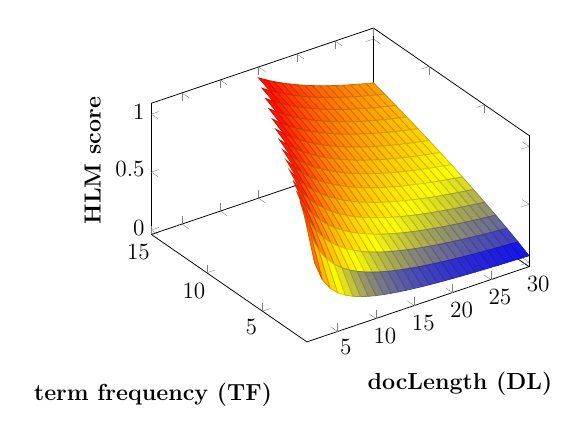
\begin{tikzpicture}[thick,scale=0.7, every node/.style={transform shape}]\begin{axis}[
 %title={},
 %y dir=reverse, 
 x dir=reverse, 
 ylabel={docLength (DL)},
 xlabel={term frequency (TF)},
 zlabel={HLM score},
 every axis/.append style={font=\large\bfseries},
 max space between ticks=25pt,
 view={55}{45}
% yticklabels={0k,100k}
 ] 

\addplot3[surf,unbounded coords=jump]
coordinates  { 
(1,1,1)	(1,2,0.621989626156165)	(1,3,0.454919792962258)	(1,4,0.359374040891899)	(1,5,0.297247211014724)	(1,6,0.253535670926196)	(1,7,0.221079004018033)	(1,8,0.196013558516919)	(1,9,0.176066673043413)	(1,10,0.159812621390807)	(1,11,0.146311067373364)	(1,12,0.134916412227099)	(1,13,0.125170566982079)	(1,14,0.116739411565573)	(1,15,0.109373476479032)	(1,16,0.102882708780262)	(1,17,0.0971197635727905)	(1,18,0.0919686374088689)	(1,19,0.0873367506721093)	(1,20,0.0831493160857265)	(1,21,0.0793452582041037)	(1,22,0.0758742071730685)	(1,23,0.0726942505286112)	(1,24,0.0697702289388661)	(1,25,0.0670724282451611)	(1,26,0.0645755642644606)	(1,27,0.0622579866277628)	(1,28,0.0601010484168879)	(1,29,0.0580886026580694)	(1,30,0.0562065968470943)

(2,1,nan)	(2,2,1)	(2,3,0.764754026855425)	(2,4,0.621989626156165)	(2,5,0.525188803416293)	(2,6,0.454919792962258)	(2,7,0.401463820946619)	(2,8,0.359374040891899)	(2,9,0.325344772119586)	(2,10,0.297247211014724)	(2,11,0.273645732434471)	(2,12,0.253535670926196)	(2,13,0.236192227775016)	(2,14,0.221079004018033)	(2,15,0.207790318869497)	(2,16,0.196013558516919)	(2,17,0.185503863863546)	(2,18,0.176066673043413)	(2,19,0.167545408836041)	(2,20,0.159812621390807)	(2,21,0.152763503490943)	(2,22,0.146311067373364)	(2,23,0.140382505990773)	(2,24,0.134916412227099)	(2,25,0.129860628668111)	(2,26,0.125170566982079)	(2,27,0.120807881316515)	(2,28,0.116739411565573)	(2,29,0.112936334492862)	(2,30,0.109373476479032)

(3,1,nan)	(3,2,nan)	(3,3,1)	(3,4,0.829048015154822)	(3,5,0.710109539528373)	(3,6,0.621989626156165)	(3,7,0.553832024650894)	(3,8,0.499422759842862)	(3,9,0.454919792962257)	(3,10,0.417807926881635)	(3,11,0.386366066808711)	(3,12,0.359374040891899)	(3,13,0.335941294228451)	(3,14,0.315401838711434)	(3,15,0.297247211014724)	(3,16,0.281082226681238)	(3,17,0.266594929740559)	(3,18,0.253535670926196)	(3,19,0.24170222203493)	(3,20,0.230928980226506)	(3,21,0.221079004018033)	(3,22,0.212038047876564)	(3,23,0.203710031952637)	(3,24,0.196013558516919)	(3,25,0.188879202656089)	(3,26,0.182247383121429)	(3,27,0.176066673043413)	(3,28,0.170292447784477)	(3,29,0.164885793792266)	(3,30,0.159812621390807)

(4,1,nan)	(4,2,nan)	(4,3,nan)	(4,4,1)	(4,5,0.865698756849)	(4,6,0.764754026855425)	(4,7,0.685727768114339)	(4,8,0.621989626156165)	(4,9,0.569391648904037)	(4,10,0.525188803416293)	(4,11,0.487483951889205)	(4,12,0.454919792962258)	(4,13,0.426497359589787)	(4,14,0.401463820946619)	(4,15,0.379240327395148)	(4,16,0.359374040891899)	(4,17,0.341505328703937)	(4,18,0.325344772119586)	(4,19,0.310656706119163)	(4,20,0.297247211014724)	(4,21,0.284955204259961)	(4,22,0.273645732434471)	(4,23,0.263204851448174)	(4,24,0.253535670926196)	(4,25,0.244555263889519)	(4,26,0.236192227775016)	(4,27,0.228384741456421)	(4,28,0.221079004018033)	(4,29,0.21422797024867)	(4,30,0.207790318869497)

(5,1,nan)	(5,2,nan)	(5,3,nan)	(5,4,nan)	(5,5,1)	(5,6,0.889395029639195)	(5,7,0.802006501749625)	(5,8,0.730958682421364)	(5,9,0.671916477367333)	(5,10,0.621989626156165)	(5,11,0.579166557783776)	(5,12,0.541998575759629)	(5,13,0.509412832924761)	(5,14,0.480596127304584)	(5,15,0.454919792962258)	(5,16,0.431889519341492)	(5,17,0.411110867606398)	(5,18,0.392264991133567)	(5,19,0.37509117467367)	(5,20,0.359374040891899)	(5,21,0.344934020239237)	(5,22,0.331620145912424)	(5,23,0.319304533618775)	(5,24,0.307878100890691)	(5,25,0.297247211014724)	(5,26,0.287331015360257)	(5,27,0.278059329323532)	(5,28,0.269370920299868)	(5,29,0.261212116904955)	(5,30,0.253535670926196)

(6,1,nan)	(6,2,nan)	(6,3,nan)	(6,4,nan)	(6,5,nan)	(6,6,1)	(6,7,0.905978015142025)	(6,8,0.829048015154822)	(6,9,0.764754026855425)	(6,10,0.710109539528373)	(6,11,0.663025388441083)	(6,12,0.621989626156165)	(6,13,0.585877328160206)	(6,14,0.553832024650894)	(6,15,0.525188803416293)	(6,16,0.499422759842862)	(6,17,0.476113452457472)	(6,18,0.454919792962257)	(6,19,0.435561928948071)	(6,20,0.417807926881635)	(6,21,0.401463820946619)	(6,22,0.386366066808711)	(6,23,0.372375742896396)	(6,24,0.359374040891899)	(6,25,0.347258720461584)	(6,26,0.335941294228451)	(6,27,0.325344772119586)	(6,28,0.315401838711434)	(6,29,0.306053368995639)	(6,30,0.297247211014724)

(7,1,nan)	(7,2,nan)	(7,3,nan)	(7,4,nan)	(7,5,nan)	(7,6,nan)	(7,7,1)	(7,8,0.918234273546841)	(7,9,0.84957794112046)	(7,10,0.79097818724873)	(7,11,0.740291378883669)	(7,12,0.695960407129887)	(7,13,0.656822585687106)	(7,14,0.621989626156165)	(7,15,0.590769615545226)	(7,16,0.562614587372231)	(7,17,0.537084283992134)	(7,18,0.513820494881042)	(7,19,0.492528496481904)	(7,20,0.472963376930536)	(7,21,0.454919792962258)	(7,22,0.438224184168835)	(7,23,0.422728776530383)	(7,24,0.408306908660429)	(7,25,0.394849349351898)	(7,26,0.382261367362921)	(7,27,0.370460378566498)	(7,28,0.359374040891899)	(7,29,0.348938699918164)	(7,30,0.339098111501629)

(8,1,nan)	(8,2,nan)	(8,3,nan)	(8,4,nan)	(8,5,nan)	(8,6,nan)	(8,7,nan)	(8,8,1)	(8,9,0.927662416106689)	(8,10,0.865698756849)	(8,11,0.811926031756413)	(8,12,0.764754026855425)	(8,13,0.722992008524866)	(8,14,0.685727768114339)	(8,15,0.652248867041359)	(8,16,0.621989626156165)	(8,17,0.594494422029448)	(8,18,0.569391648904037)	(8,19,0.546374852391064)	(8,20,0.525188803416293)	(8,21,0.505619048373122)	(8,22,0.487483951889205)	(8,23,0.470628557307152)	(8,24,0.454919792962258)	(8,25,0.440242688612257)	(8,26,0.426497359589787)	(8,27,0.4135965811041)	(8,28,0.401463820946619)	(8,29,0.390031631699611)	(8,30,0.379240327395148)

(9,1,nan)	(9,2,nan)	(9,3,nan)	(9,4,nan)	(9,5,nan)	(9,6,nan)	(9,7,nan)	(9,8,nan)	(9,9,1)	(9,10,0.935140381695894)	(9,11,0.878694731064694)	(9,12,0.829048015154822)	(9,13,0.784988233279183)	(9,14,0.745584847988371)	(9,15,0.710109539528373)	(9,16,0.677982799728178)	(9,17,0.648736907108141)	(9,18,0.621989626156165)	(9,19,0.597425124783112)	(9,20,0.574779869158577)	(9,21,0.553832024650894)	(9,22,0.53439337361256)	(9,23,0.516303070640622)	(9,24,0.499422759842862)	(9,25,0.483632715624168)	(9,26,0.468828762278324)	(9,27,0.454919792962257)	(9,28,0.441825754802413)	(9,29,0.429476000001598)	(9,30,0.417807926881635)

(10,1,nan)	(10,2,nan)	(10,3,nan)	(10,4,nan)	(10,5,nan)	(10,6,nan)	(10,7,nan)	(10,8,nan)	(10,9,nan)	(10,10,1)	(10,11,0.941216700120071)	(10,12,0.889395029639195)	(10,13,0.843306569506414)	(10,14,0.802006501749625)	(10,15,0.764754026855425)	(10,16,0.730958682421364)	(10,17,0.700143092024258)	(10,18,0.671916477367333)	(10,19,0.645955420048794)	(10,20,0.621989626156165)	(10,21,0.599791217686162)	(10,22,0.579166557783776)	(10,23,0.559949927437822)	(10,24,0.541998575759629)	(10,25,0.525188803416293)	(10,26,0.509412832924761)	(10,27,0.494576285093826)	(10,28,0.480596127304584)	(10,29,0.467398992623918)	(10,30,0.454919792962258)

(11,1,nan)	(11,2,nan)	(11,3,nan)	(11,4,nan)	(11,5,nan)	(11,6,nan)	(11,7,nan)	(11,8,nan)	(11,9,nan)	(11,10,nan)	(11,11,1)	(11,12,0.946251773773493)	(11,13,0.898359063783389)	(11,14,0.855365760866882)	(11,15,0.816521122996797)	(11,16,0.781225898364072)	(11,17,0.748994911755086)	(11,18,0.719430440936898)	(11,19,0.692202864399309)	(11,20,0.667036329703138)	(11,21,0.643697963281252)	(11,22,0.621989626156165)	(11,23,0.601741531169737)	(11,24,0.582807242194464)	(11,25,0.56505971354562)	(11,26,0.548388122191579)	(11,27,0.532695311135566)	(11,28,0.517895708902828)	(11,29,0.50391362349877)	(11,30,0.490681833524032)

(12,1,nan)	(12,2,nan)	(12,3,nan)	(12,4,nan)	(12,5,nan)	(12,6,nan)	(12,7,nan)	(12,8,nan)	(12,9,nan)	(12,10,nan)	(12,11,nan)	(12,12,1)	(12,13,0.950492175929015)	(12,14,0.905978015142025)	(12,15,0.865698756849)	(12,16,0.829048015154822)	(12,17,0.795534246685824)	(12,18,0.764754026855425)	(12,19,0.736372612793849)	(12,20,0.710109539528373)	(12,21,0.685727768114339)	(12,22,0.663025388441083)	(12,23,0.641829190890472)	(12,24,0.621989626156165)	(12,25,0.603376810486853)	(12,26,0.585877328160206)	(12,27,0.569391648904037)	(12,28,0.553832024650894)	(12,29,0.539120763532788)	(12,30,0.525188803416293)

(13,1,nan)	(13,2,nan)	(13,3,nan)	(13,4,nan)	(13,5,nan)	(13,6,nan)	(13,7,nan)	(13,8,nan)	(13,9,nan)	(13,10,nan)	(13,11,nan)	(13,12,nan)	(13,13,1)	(13,14,0.954112309123327)	(13,15,0.912533690996205)	(13,16,0.874651908858968)	(13,17,0.839970168196483)	(13,18,0.808080318070828)	(13,19,0.778643350080918)	(13,20,0.751374939708565)	(13,21,0.726034547264215)	(13,22,0.702417079939828)	(13,23,0.680346428146221)	(13,24,0.659670394616598)	(13,25,0.640256672853748)	(13,26,0.621989626156165)	(13,27,0.604767684461415)	(13,28,0.588501222991279)	(13,29,0.573110820266669)	(13,30,0.55852581750597)

(14,1,nan)	(14,2,nan)	(14,3,nan)	(14,4,nan)	(14,5,nan)	(14,6,nan)	(14,7,nan)	(14,8,nan)	(14,9,nan)	(14,10,nan)	(14,11,nan)	(14,12,nan)	(14,13,nan)	(14,14,1)	(14,15,0.957239013621133)	(14,16,0.918234273546841)	(14,17,0.882484616547527)	(14,18,0.84957794112046)	(14,19,0.819171657582869)	(14,20,0.79097818724873)	(14,21,0.764754026855425)	(14,22,0.740291378883669)	(14,23,0.717411660231811)	(14,24,0.695960407129887)	(14,25,0.675803232372462)	(14,26,0.656822585687106)	(14,27,0.638915134124429)	(14,28,0.621989626156165)	(14,29,0.60596513679652)	(14,30,0.590769615545226)

(15,1,nan)	(15,2,nan)	(15,3,nan)	(15,4,nan)	(15,5,nan)	(15,6,nan)	(15,7,nan)	(15,8,nan)	(15,9,nan)	(15,10,nan)	(15,11,nan)	(15,12,nan)	(15,13,nan)	(15,14,nan)	(15,15,1)	(15,16,0.959966748341296)	(15,17,0.92323690127406)	(15,18,0.889395029639195)	(15,19,0.85809551482511)	(15,20,0.829048015154822)	(15,21,0.802006501749625)	(15,22,0.776760863890398)	(15,23,0.753130395817862)	(15,24,0.730958682421364)	(15,25,0.710109539528373)	(15,26,0.690463759301656)	(15,27,0.671916477367333)	(15,28,0.654375025136852)	(15,29,0.637757164447431)	(15,30,0.621989626156165)

}; \end{axis} \end{tikzpicture}

       	\label{cTFVSDL15}
    \end{subfigure}  
      ~
     \begin{subfigure}[b]{0.5\textwidth}
      \centering
      \caption{TF vs, Doc. Length (DL)  with $c = 0.99$}
       
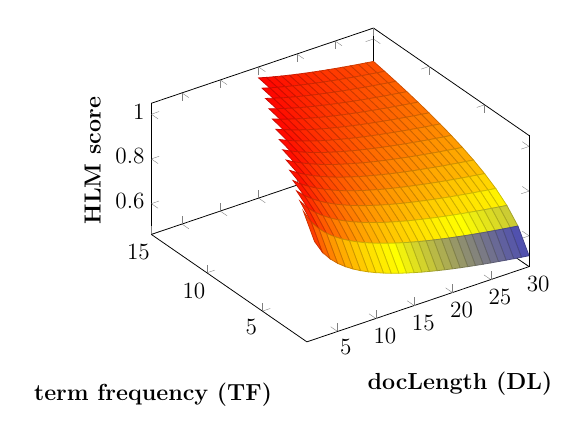
\begin{tikzpicture}[thick,scale=0.7, every node/.style={transform shape}]\begin{axis}[
%title={},
%y dir=reverse, 
x dir=reverse, 
ylabel={docLength (DL)},
xlabel={term frequency (TF)},
zlabel={HLM score},
every axis/.append style={font=\large\bfseries},
max space between ticks=25pt,
view={55}{45}
% yticklabels={0k,100k}
] 

\addplot3[surf,unbounded coords=jump]
coordinates  { 
(1,1,1)	(1,2,0.899671365707223)	(1,3,0.841043406928067)	(1,4,0.799488487034831)	(1,5,0.767288572151157)	(1,6,0.741005844337785)	(1,7,0.718806466948285)	(1,8,0.699595803046279)	(1,9,0.682667789466625)	(1,10,0.667540331328603)	(1,11,0.653869570058235)	(1,12,0.64140161327701)	(1,13,0.629943652382547)	(1,14,0.619345814263553)	(1,15,0.609489289412862)	(1,16,0.600278299357417)	(1,17,0.591634503551573)	(1,18,0.583493007386208)	(1,19,0.575799450958578)	(1,20,0.568507845449242)	(1,21,0.561578937933734)	(1,22,0.554978956939974)	(1,23,0.548678637082807)	(1,24,0.542652451434819)	(1,25,0.536878000702402)	(1,26,0.531335522273925)	(1,27,0.526007491973526)	(1,28,0.520878298276225)	(1,29,0.515933973717023)	(1,30,0.511161971852579)

(2,1,nan)	(2,2,1)	(2,3,0.941299108339227)	(2,4,0.899671365707223)	(2,5,0.867398737969139)	(2,6,0.841043406928067)	(2,7,0.818771535680754)	(2,8,0.799488487034831)	(2,9,0.782488197569988)	(2,10,0.767288572151157)	(2,11,0.753545751950832)	(2,12,0.741005844337785)	(2,13,0.729476040457734)	(2,14,0.718806466948285)	(2,15,0.708878314051983)	(2,16,0.699595803046279)	(2,17,0.690880593136834)	(2,18,0.682667789466625)	(2,19,0.674903031885802)	(2,20,0.667540331328603)	(2,21,0.660540434625025)	(2,22,0.653869570058235)	(2,23,0.647498471999103)	(2,24,0.64140161327701)	(2,25,0.635556594355922)	(2,26,0.629943652382547)	(2,27,0.624545262940128)	(2,28,0.619345814263553)	(2,29,0.61433133864845)	(2,30,0.609489289412862)

(3,1,nan)	(3,2,nan)	(3,3,1)	(3,4,0.958347925979563)	(3,5,0.926050987289633)	(3,6,0.899671365707223)	(3,7,0.877375224303047)	(3,8,0.858067925858746)	(3,9,0.841043406928067)	(3,10,0.825819572350041)	(3,11,0.812052563271309)	(3,12,0.799488487034831)	(3,13,0.78793453476056)	(3,14,0.77724083306038)	(3,15,0.767288572151157)	(3,16,0.75798197328471)	(3,17,0.749242695641108)	(3,18,0.741005844337785)	(3,19,0.733217059199386)	(3,20,0.725830351134692)	(3,21,0.718806466948285)	(3,22,0.712111634897961)	(3,23,0.705716589329259)	(3,24,0.699595803046279)	(3,25,0.693726876487745)	(3,26,0.688090046775164)	(3,27,0.682667789466625)	(3,28,0.677444492771904)	(3,29,0.672406188961558)	(3,30,0.667540331328603)

(4,1,nan)	(4,2,nan)	(4,3,nan)	(4,4,1)	(4,5,0.967690892037064)	(4,6,0.941299108339227)	(4,7,0.918990811970849)	(4,8,0.899671365707223)	(4,9,0.882634706095753)	(4,10,0.867398737969139)	(4,11,0.853619602467696)	(4,12,0.841043406928067)	(4,13,0.829477342463892)	(4,14,0.818771535680754)	(4,15,0.808807176789224)	(4,16,0.799488487034831)	(4,17,0.790737125591366)	(4,18,0.782488197569988)	(4,19,0.774687342789078)	(4,20,0.767288572151157)	(4,21,0.760252632454558)	(4,22,0.753545751950832)	(4,23,0.747138664979285)	(4,24,0.741005844337785)	(4,25,0.735124890458836)	(4,26,0.729476040457734)	(4,27,0.724041769886358)	(4,28,0.718806466948285)	(4,29,0.713756163907883)	(4,30,0.708878314051983)

(5,1,nan)	(5,2,nan)	(5,3,nan)	(5,4,nan)	(5,5,1)	(5,6,0.973600913633586)	(5,7,0.951285317910699)	(5,8,0.931958575604364)	(5,9,0.914914623259726)	(5,10,0.899671365707223)	(5,11,0.88588494408491)	(5,12,0.873301465727175)	(5,13,0.861728121745405)	(5,14,0.851015038742928)	(5,15,0.841043406928067)	(5,16,0.831717447544101)	(5,17,0.822958819762576)	(5,18,0.814702628692406)	(5,19,0.80689451414973)	(5,20,0.799488487034831)	(5,21,0.792445294143802)	(5,22,0.785731163725958)	(5,23,0.779316830118372)	(5,24,0.773176766116681)	(5,25,0.767288572151157)	(5,26,0.761632485334869)	(5,27,0.756190981217471)	(5,28,0.750948448000317)	(5,29,0.745890917945551)	(5,30,0.741005844337785)

(6,1,nan)	(6,2,nan)	(6,3,nan)	(6,4,nan)	(6,5,nan)	(6,6,1)	(6,7,0.977679535381201)	(6,8,0.958347925979563)	(6,9,0.941299108339227)	(6,10,0.926050987289633)	(6,11,0.912259703967836)	(6,12,0.899671365707223)	(6,13,0.888093163618182)	(6,14,0.877375224303047)	(6,15,0.867398737969139)	(6,16,0.858067925858746)	(6,17,0.849304447142415)	(6,18,0.841043406928067)	(6,19,0.833230445030845)	(6,20,0.825819572350041)	(6,21,0.818771535680754)	(6,22,0.812052563271309)	(6,23,0.805633389457785)	(6,24,0.799488487034831)	(6,25,0.79359545643173)	(6,26,0.78793453476056)	(6,27,0.782488197569988)	(6,28,0.77724083306038)	(6,29,0.772178473492895)	(6,30,0.767288572151157)

(7,1,nan)	(7,2,nan)	(7,3,nan)	(7,4,nan)	(7,5,nan)	(7,6,nan)	(7,7,1)	(7,8,0.980664912598375)	(7,9,0.963612618043915)	(7,10,0.948361021165549)	(7,11,0.934566263099823)	(7,12,0.921974451179616)	(7,13,0.910392776514808)	(7,14,0.899671365707223)	(7,15,0.889691408963676)	(7,16,0.880357127525945)	(7,17,0.871590180564072)	(7,18,0.863325673185471)	(7,19,0.855509245204779)	(7,20,0.848094907520779)	(7,21,0.841043406928067)	(7,22,0.834320971674459)	(7,23,0.827898336095533)	(7,24,0.82174997298543)	(7,25,0.815853482772928)	(7,26,0.810189102569603)	(7,27,0.804739307923617)	(7,28,0.799488487034831)	(7,29,0.794422672163902)	(7,30,0.789529316593951)

(8,1,nan)	(8,2,nan)	(8,3,nan)	(8,4,nan)	(8,5,nan)	(8,6,nan)	(8,7,nan)	(8,8,1)	(8,9,0.982945096828066)	(8,10,0.967690892037064)	(8,11,0.953893526763254)	(8,12,0.941299108339227)	(8,13,0.92971482787458)	(8,14,0.918990811970849)	(8,15,0.909008250834566)	(8,16,0.899671365707223)	(8,17,0.890901815758575)	(8,18,0.882634706095753)	(8,19,0.874815676533108)	(8,20,0.867398737969139)	(8,21,0.860344637198157)	(8,22,0.853619602467696)	(8,23,0.847194368113046)	(8,24,0.841043406928067)	(8,25,0.835144319341251)	(8,26,0.829477342463892)	(8,27,0.824024951843867)	(8,28,0.818771535680754)	(8,29,0.813703126234927)	(8,30,0.808807176789224)

(9,1,nan)	(9,2,nan)	(9,3,nan)	(9,4,nan)	(9,5,nan)	(9,6,nan)	(9,7,nan)	(9,8,nan)	(9,9,1)	(9,10,0.984743766215252)	(9,11,0.970944372430966)	(9,12,0.958347925979563)	(9,13,0.946761617970464)	(9,14,0.936035575005035)	(9,15,0.926050987289633)	(9,16,0.91671207606558)	(9,17,0.907940500502457)	(9,18,0.899671365707223)	(9,19,0.891850311494057)	(9,20,0.884431348761285)	(9,21,0.877375224303047)	(9,22,0.870648166366704)	(9,23,0.864220909287374)	(9,24,0.858067925858746)	(9,25,0.852166816509141)	(9,26,0.846497818349679)	(9,27,0.841043406928067)	(9,28,0.835787970443711)	(9,29,0.830717541156813)	(9,30,0.825819572350041)

(10,1,nan)	(10,2,nan)	(10,3,nan)	(10,4,nan)	(10,5,nan)	(10,6,nan)	(10,7,nan)	(10,8,nan)	(10,9,nan)	(10,10,1)	(10,11,0.986198982977501)	(10,12,0.973600913633586)	(10,13,0.962012983077567)	(10,14,0.951285317910699)	(10,15,0.941299108339227)	(10,16,0.931958575604364)	(10,17,0.923185378875581)	(10,18,0.914914623259726)	(10,19,0.907091948570867)	(10,20,0.899671365707223)	(10,21,0.892613621462819)	(10,22,0.88588494408491)	(10,23,0.879456067908503)	(10,24,0.873301465727175)	(10,25,0.867398737969139)	(10,26,0.861728121745405)	(10,27,0.856272092603569)	(10,28,0.851015038742928)	(10,29,0.845942992423575)	(10,30,0.841043406928067)

(11,1,nan)	(11,2,nan)	(11,3,nan)	(11,4,nan)	(11,5,nan)	(11,6,nan)	(11,7,nan)	(11,8,nan)	(11,9,nan)	(11,10,nan)	(11,11,1)	(11,12,0.987400602523669)	(11,13,0.975811344091026)	(11,14,0.965082351303253)	(11,15,0.955094814366521)	(11,16,0.945752954521968)	(11,17,0.936978430938991)	(11,18,0.928706348724365)	(11,19,0.920882347692086)	(11,20,0.913460438740296)	(11,21,0.906401368662948)	(11,22,0.899671365707223)	(11,23,0.893241164208054)	(11,24,0.887085236958944)	(11,25,0.881181184388034)	(11,26,0.875509243606258)	(11,27,0.870051890161141)	(11,28,0.864793512251906)	(11,29,0.859720142138569)	(11,30,0.854819233103617)

(12,1,nan)	(12,2,nan)	(12,3,nan)	(12,4,nan)	(12,5,nan)	(12,6,nan)	(12,7,nan)	(12,8,nan)	(12,9,nan)	(12,10,nan)	(12,11,nan)	(12,12,1)	(12,13,0.988409634770886)	(12,14,0.977679535381201)	(12,15,0.967690892037064)	(12,16,0.958347925979563)	(12,17,0.949572296378043)	(12,18,0.941299108339227)	(12,19,0.93347400167706)	(12,20,0.926050987289633)	(12,21,0.918990811970849)	(12,22,0.912259703967836)	(12,23,0.905828397615476)	(12,24,0.899671365707223)	(12,25,0.893766208671163)	(12,26,0.888093163618182)	(12,27,0.882634706095753)	(12,28,0.877375224303047)	(12,29,0.872300750500031)	(12,30,0.867398737969139)

(13,1,nan)	(13,2,nan)	(13,3,nan)	(13,4,nan)	(13,5,nan)	(13,6,nan)	(13,7,nan)	(13,8,nan)	(13,9,nan)	(13,10,nan)	(13,11,nan)	(13,12,nan)	(13,13,1)	(13,14,0.989268964076458)	(13,15,0.979279384349882)	(13,16,0.969935482061322)	(13,17,0.961158916380088)	(13,18,0.952884792412865)	(13,19,0.945058749973562)	(13,20,0.937634799960232)	(13,21,0.930573689166742)	(13,22,0.923841645840184)	(13,23,0.917409404315403)	(13,24,0.911251437385816)	(13,25,0.905345345479473)	(13,26,0.899671365707223)	(13,27,0.894211973616501)	(13,28,0.888951557406445)	(13,29,0.883876149336982)	(13,30,0.878973202690511)

(14,1,nan)	(14,2,nan)	(14,3,nan)	(14,4,nan)	(14,5,nan)	(14,6,nan)	(14,7,nan)	(14,8,nan)	(14,9,nan)	(14,10,nan)	(14,11,nan)	(14,12,nan)	(14,13,nan)	(14,14,1)	(14,15,0.990009617520106)	(14,16,0.980664912598375)	(14,17,0.971887544404093)	(14,18,0.963612618043915)	(14,19,0.955785773331725)	(14,20,0.948361021165549)	(14,21,0.941299108339227)	(14,22,0.934566263099823)	(14,23,0.928133219782156)	(14,24,0.921974451179616)	(14,25,0.916067557720226)	(14,26,0.910392776514808)	(14,27,0.90493258311077)	(14,28,0.899671365707223)	(14,29,0.894595156564068)	(14,30,0.889691408963676)

(15,1,nan)	(15,2,nan)	(15,3,nan)	(15,4,nan)	(15,5,nan)	(15,6,nan)	(15,7,nan)	(15,8,nan)	(15,9,nan)	(15,10,nan)	(15,11,nan)	(15,12,nan)	(15,13,nan)	(15,14,nan)	(15,15,1)	(15,16,0.99065459935127)	(15,17,0.981876535526919)	(15,18,0.973600913633586)	(15,19,0.965773373485132)	(15,20,0.958347925979563)	(15,21,0.951285317910699)	(15,22,0.944551777525583)	(15,23,0.938118039159015)	(15,24,0.931958575604364)	(15,25,0.926050987289633)	(15,26,0.920375511325624)	(15,27,0.914914623259726)	(15,28,0.909652711291026)	(15,29,0.904575807679408)	(15,30,0.899671365707223)

}; \end{axis} \end{tikzpicture}

       \label{cTFVSDL99}
    \end{subfigure}  
    \caption{HLM analysis}
	\label{cTFVSDL}
\end{figure}

Figure \ref{hlm-ctf-dl} shows HLM scores with respect to ``collection term frequency (CTF)\footnote{Also known as ``document frequency''}'' and document length (DL). 

For documents where the length is lower than 5, the differences between the scores are very marked, whereas out-with that range the progression of the scores is much more subtle. In other words, short documents such as microblogs are subject to a high impact in their scores due to small changes in their limited length. As it can be observed in Formula \ref{hlmformula}, this sensitivity to document length is a result of the model's design, since document length acts as a multiplier in the denominator. 

In addition, within the nominator we find term frequency as a multiplying component. Consequently, when higher than 1 it will result in an unreasonable boost of the score. In the case of microblog documents this can be problematic due to the scarce frequencies which average around 1.17 ($\pm 0.48$)\footnote{Computed for query terms in all TREC microblog topics up to 2014 and our baseline DFR}.
 
%To further illustrate these differences, we introduce Figure \ref{hlmcomp} where we show HLM scores w.r.t. term frequency ($f(q_i, D)$) within the 1 to 10 range. All other variables are kept constant\footnote{($c = 0.15$, $f(q_i, C) = 100$, $|D| = 5$ and $ntoks = 1000$)}.
%
%\begin{figure}[]
%  \centering
%   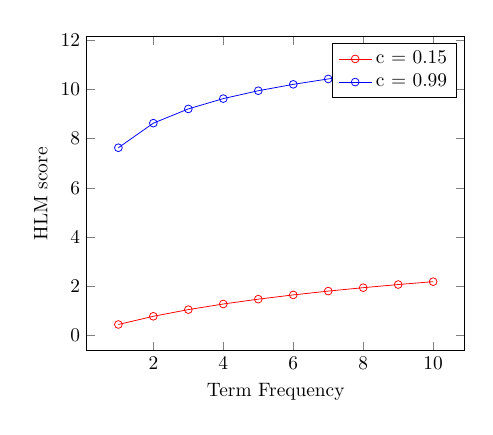
\begin{tikzpicture}[thick,scale=0.7, every node/.style={transform shape}]
	\begin{axis}[
		xlabel=Term Frequency,
		ylabel=HLM score]
	\addplot[color=red,mark=o] coordinates {
		(1,0.436)
		(2,0.770)
		(3,1.041)
		(4,1.270)
		(5,1.467)
		(6,1.640)
		(7,1.795)
		(8,1.934)
		(9,2.062)
		(10,2.179)
	};
	\addlegendentry{c = 0.15}
	\addplot[color=blue,mark=o] coordinates {
		(1,	7.63)
		(2,8.63)
		(3,9.21)
		(4,9.63)
		(5,9.95)
		(6,10.21)
		(7,10.43)
		(8,10.63)
		(9,10.80)
		(10,11.08)
		};
	\addlegendentry{c = 0.99}
	\end{axis}
%	7.6366
%	8.6330
%	9.2167
%	9.6312
%	9.9527
%	10.2155
%	10.4378
%	10.6303
%	10.8001
%	10.9520
%	11.0895
	
\end{tikzpicture}

%     \caption{TF vs HLM Score}
%  \label{hlmcomp}
%\end{figure}
%
%As we can observe in Figure \ref{hlmcomp}, the low term frequencies show substantial differences between the scores. As term frequencies grow the differences between scores become increasingly smaller. The intuition is that for documents of the same length, documents with higher query term frequency should be ranked higher. Unfortunately, for very low query term frequencies the score differences introduced by design for this purpose are too aggressive, and very unlikely correspond to the actual importance of such frequency differences.

Table \ref{traditional} shows that HLM is the second worst model overall for microblog retrieval. We hypothesise that the reason for this under-performance lies in the substantial scoring differences above-mentioned, resulting from the specific morphology of microblog documents.

In order to test this hypotheses we set to overestimate the vales for within document query term frequency (TF) as well as the actual document length (DL). We do this by a simple addition \(TF = TF+dTF\), in this case \(dTF\) being the pondering value to overestimate \(TF\). Likewise, we utilise \(DL = DL+dDL\) where \(dDL\) is the variable to over-estimate \(DL\).

Table \ref{hlmOverestimates} shows the performance of HLM measured by Precision@30 with different configurations. The first row shows the performance of HLM with a default configuration of $c = 0.15$. 

\begin{table}[]

	\caption{P@30 scores for HLM as we consider different combinations of dTF and dDL, and c}
	\centering
	\begin{tabular}{l|c|c|c} 	
	\textit{\textbf{c}} & 
	\textit{\textbf{dTF}} & 
	\textit{\textbf{dDL}} & 
	\textit{\textbf{P@30}} 	
	\tabularnewline
	\hline
	0.15 &    &    & 0.3475\\
	0.15 & 20 &    & 0.3486\\
	0.15 &    & 20 & \textbf{0.3839} \\
	0.15 & 20 & 20 & \textbf{0.4462} \\
	\hline
	\hline
	0.05 &  &  & \textbf{0.2824} \\
	0.40 &  &  & \textbf{0.4009} \\
	0.70 &  &  & \textbf{0.4281} \\
	0.99 &  &  & \textbf{0.4492} \\
	\hline
    \hline
	0.99 & 20 & 20 & \textbf{0.4532} \\	
	\hline
	\end{tabular}
	\label{hlmOverestimates}
\end{table}

The second row with $dTF = 20$ so that $TF = TF+20$ which denotes the overestimation of TF by +20. As stated before, the reason behind this overestimation is to reduce the differences between scores with respect to the different real values of TF. As we can observe only overestimating TF does no result in any significant improvement.

Similarly, the third row shows the performance of HLM when overestimating DL by +20 in order to reduce the effects in the score due to DL differences. As consequence the results are much better than before with a Precision@30 increase of +11.76\%. 

Finally, we test the overestimation of TF and DL together to achieve yet another +15.79\% Precision@30 increase over the previous combination and a very substantial increase of +29.41\% over the baseline configuration. It is interesting to notice how only the increase of TF does not help in retrieval, however only increasing DL does produce better results. More importantly, by incrementing both TF and DL we obtain the best performance over all previous configurations.

These results hint to a very subtle relationship between DL and TF values of microblog documents. Rows 5 to 8 in Table \ref{hlmOverestimates} show the performance of HLM with different values of $c$. As $c$ is increased performance increases as well, reaching comparable performance to the approach which overestimates DL and TF. If we look back at Figure \ref{hlmcomp} we find that as $c$ is becomes higher so do the differences in score with respect to TF. This finding on its own contradicts our hypotheses, however this is not the whole picture.


Figures \ref{cTFVSDL15} and \ref{cTFVSDL99} show scores produced by HLM w.r.t. TF and DL. Figure \ref{cTFVSDL15} sets $c=0.15$ whereas Figure \ref{cTFVSDL99} sets $c=0.99$. It is easily observed how the HLM scores differ between the two figures. Moreover Figure \ref{cTFVSDL15} shows more differences across the spectrum of scores with respect to TF and DL than Figure \ref{cTFVSDL99}. We can also observe how over-estimating DL and TF forces the values of HLM to lie in the more stable area of the Figures. Furthermore, Figure \ref{cTFVSDL99} produces the most stable scores, even when the progression of values with respect to TF may be slightly more abrupt at lower TF points.

We can conclude from these results that retrieving microblogs requires a conservative, delicate and balanced estimation of the importance of TF and DL.

\todo{First notion of gentle slope}

\subsection{The DLM Case}
Dirichlet Smoothed language model (DLM), was the baseline retrieval model for the 2013 and 2014 iterations of the microblog track, within the "Microblog track as a service" client. DLM has a smoothing parameter named $\mu$, which was set to 2500 by default during the 2013 and 2014 microblog tracks. Moreover, DLM scores are produced \footnote{As implemented in the Terrier IR platform} by the following equation:

\begin{small}
\begin{align}
\label{dlmformula}
    \text{DLM}(D,Q) &= \sum_{i=1}^{n} \log_2 \left[ 1 + \frac{f(q_i, D)}{\mu \cdot \frac{ f(q_i, C) }{ ntoks }}\right] + \log_2 \left[\frac{\mu}{|D| + \mu}\right]
\end{align}
\label{dlmequation}
%\end{proof}
\end{small}

\noindent where $ntoks$ refers to the number of unique tokens in the collection (NT), $\mu$ is a free parameter, and $C$ represents the set of all documents in the collection. $f(q_i, D)$ represents the TF of a query term $q_i$ in document $D$, whereas $f(q_i, C)$ is the collection document frequency (CTF) of term $q_i$.

\begin{figure}
 		\begin{subfigure}[]{0.5\textwidth}
     	\caption{Document Frequency and $\mu$ parameter} 
    	
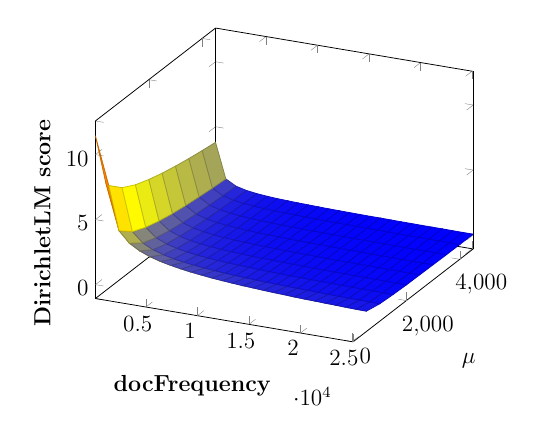
\begin{tikzpicture}[thick,scale=0.7, every node/.style={transform shape}]\begin{axis}[
 %title={},
 %y dir=reverse, 
 %x dir=reverse, 
 ylabel={$\mu$},
 xlabel={docFrequency},
 zlabel={DirichletLM score},
 every axis/.append style={font=\large\bfseries},
 max space between ticks=25pt
% yticklabels={0k,100k}
 ] 

		\addplot3[surf] coordinates { 
%patch,patch type=biquadratic, shader=faceted,patch refines=3
(100.00,1.00,11.45)(100.00,501.00,6.83)(100.00,1001.00,5.87)(100.00,1501.00,5.30)(100.00,2001.00,4.91)(100.00,2501.00,4.60)(100.00,3001.00,4.35)(100.00,3501.00,4.14)(100.00,4001.00,3.96)(100.00,4501.00,3.80)

(1100.00,1.00,7.99)(1100.00,501.00,3.48)(1100.00,1001.00,2.63)(1100.00,1501.00,2.17)(1100.00,2001.00,1.86)(1100.00,2501.00,1.63)(1100.00,3001.00,1.46)(1100.00,3501.00,1.33)(1100.00,4001.00,1.21)(1100.00,4501.00,1.12)

(2100.00,1.00,7.05)(2100.00,501.00,2.66)(2100.00,1001.00,1.89)(2100.00,1501.00,1.50)(2100.00,2001.00,1.25)(2100.00,2501.00,1.07)(2100.00,3001.00,0.94)(2100.00,3501.00,0.84)(2100.00,4001.00,0.76)(2100.00,4501.00,0.69)

(3100.00,1.00,6.49)(3100.00,501.00,2.20)(3100.00,1001.00,1.50)(3100.00,1501.00,1.16)(3100.00,2001.00,0.95)(3100.00,2501.00,0.80)(3100.00,3001.00,0.70)(3100.00,3501.00,0.61)(3100.00,4001.00,0.55)(3100.00,4501.00,0.50)

(4100.00,1.00,6.09)(4100.00,501.00,1.89)(4100.00,1001.00,1.25)(4100.00,1501.00,0.95)(4100.00,2001.00,0.76)(4100.00,2501.00,0.64)(4100.00,3001.00,0.55)(4100.00,3501.00,0.49)(4100.00,4001.00,0.43)(4100.00,4501.00,0.39)

(5100.00,1.00,5.78)(5100.00,501.00,1.66)(5100.00,1001.00,1.07)(5100.00,1501.00,0.80)(5100.00,2001.00,0.64)(5100.00,2501.00,0.53)(5100.00,3001.00,0.46)(5100.00,3501.00,0.40)(5100.00,4001.00,0.36)(5100.00,4501.00,0.32)

(6100.00,1.00,5.52)(6100.00,501.00,1.49)(6100.00,1001.00,0.94)(6100.00,1501.00,0.69)(6100.00,2001.00,0.55)(6100.00,2501.00,0.46)(6100.00,3001.00,0.39)(6100.00,3501.00,0.34)(6100.00,4001.00,0.30)(6100.00,4501.00,0.27)

(7100.00,1.00,5.30)(7100.00,501.00,1.35)(7100.00,1001.00,0.84)(7100.00,1501.00,0.61)(7100.00,2001.00,0.48)(7100.00,2501.00,0.40)(7100.00,3001.00,0.34)(7100.00,3501.00,0.30)(7100.00,4001.00,0.26)(7100.00,4501.00,0.24)

(8100.00,1.00,5.11)(8100.00,501.00,1.23)(8100.00,1001.00,0.76)(8100.00,1501.00,0.55)(8100.00,2001.00,0.43)(8100.00,2501.00,0.36)(8100.00,3001.00,0.30)(8100.00,3501.00,0.26)(8100.00,4001.00,0.23)(8100.00,4501.00,0.21)

(9100.00,1.00,4.94)(9100.00,501.00,1.14)(9100.00,1001.00,0.69)(9100.00,1501.00,0.50)(9100.00,2001.00,0.39)(9100.00,2501.00,0.32)(9100.00,3001.00,0.27)(9100.00,3501.00,0.24)(9100.00,4001.00,0.21)(9100.00,4501.00,0.19)

(10100.00,1.00,4.79)(10100.00,501.00,1.05)(10100.00,1001.00,0.63)(10100.00,1501.00,0.45)(10100.00,2001.00,0.35)(10100.00,2501.00,0.29)(10100.00,3001.00,0.25)(10100.00,3501.00,0.21)(10100.00,4001.00,0.19)(10100.00,4501.00,0.17)

(11100.00,1.00,4.65)(11100.00,501.00,0.98)(11100.00,1001.00,0.58)(11100.00,1501.00,0.42)(11100.00,2001.00,0.32)(11100.00,2501.00,0.26)(11100.00,3001.00,0.22)(11100.00,3501.00,0.19)(11100.00,4001.00,0.17)(11100.00,4501.00,0.15)

(12100.00,1.00,4.53)(12100.00,501.00,0.92)(12100.00,1001.00,0.54)(12100.00,1501.00,0.38)(12100.00,2001.00,0.30)(12100.00,2501.00,0.24)(12100.00,3001.00,0.21)(12100.00,3501.00,0.18)(12100.00,4001.00,0.16)(12100.00,4501.00,0.14)

(13100.00,1.00,4.42)(13100.00,501.00,0.86)(13100.00,1001.00,0.50)(13100.00,1501.00,0.36)(13100.00,2001.00,0.28)(13100.00,2501.00,0.23)(13100.00,3001.00,0.19)(13100.00,3501.00,0.17)(13100.00,4001.00,0.15)(13100.00,4501.00,0.13)

(14100.00,1.00,4.31)(14100.00,501.00,0.82)(14100.00,1001.00,0.47)(14100.00,1501.00,0.33)(14100.00,2001.00,0.26)(14100.00,2501.00,0.21)(14100.00,3001.00,0.18)(14100.00,3501.00,0.15)(14100.00,4001.00,0.14)(14100.00,4501.00,0.12)

(15100.00,1.00,4.21)(15100.00,501.00,0.77)(15100.00,1001.00,0.44)(15100.00,1501.00,0.31)(15100.00,2001.00,0.24)(15100.00,2501.00,0.20)(15100.00,3001.00,0.17)(15100.00,3501.00,0.14)(15100.00,4001.00,0.13)(15100.00,4501.00,0.11)

(16100.00,1.00,4.12)(16100.00,501.00,0.73)(16100.00,1001.00,0.42)(16100.00,1501.00,0.29)(16100.00,2001.00,0.23)(16100.00,2501.00,0.18)(16100.00,3001.00,0.16)(16100.00,3501.00,0.13)(16100.00,4001.00,0.12)(16100.00,4501.00,0.11)

(17100.00,1.00,4.03)(17100.00,501.00,0.70)(17100.00,1001.00,0.40)(17100.00,1501.00,0.28)(17100.00,2001.00,0.21)(17100.00,2501.00,0.17)(17100.00,3001.00,0.15)(17100.00,3501.00,0.13)(17100.00,4001.00,0.11)(17100.00,4501.00,0.10)

(18100.00,1.00,3.95)(18100.00,501.00,0.66)(18100.00,1001.00,0.38)(18100.00,1501.00,0.26)(18100.00,2001.00,0.20)(18100.00,2501.00,0.16)(18100.00,3001.00,0.14)(18100.00,3501.00,0.12)(18100.00,4001.00,0.11)(18100.00,4501.00,0.09)

(19100.00,1.00,3.87)(19100.00,501.00,0.63)(19100.00,1001.00,0.36)(19100.00,1501.00,0.25)(19100.00,2001.00,0.19)(19100.00,2501.00,0.16)(19100.00,3001.00,0.13)(19100.00,3501.00,0.11)(19100.00,4001.00,0.10)(19100.00,4501.00,0.09)

(20100.00,1.00,3.80)(20100.00,501.00,0.61)(20100.00,1001.00,0.34)(20100.00,1501.00,0.24)(20100.00,2001.00,0.18)(20100.00,2501.00,0.15)(20100.00,3001.00,0.12)(20100.00,3501.00,0.11)(20100.00,4001.00,0.09)(20100.00,4501.00,0.08)

(21100.00,1.00,3.73)(21100.00,501.00,0.58)(21100.00,1001.00,0.32)(21100.00,1501.00,0.23)(21100.00,2001.00,0.17)(21100.00,2501.00,0.14)(21100.00,3001.00,0.12)(21100.00,3501.00,0.10)(21100.00,4001.00,0.09)(21100.00,4501.00,0.08)

(22100.00,1.00,3.66)(22100.00,501.00,0.56)(22100.00,1001.00,0.31)(22100.00,1501.00,0.22)(22100.00,2001.00,0.17)(22100.00,2501.00,0.13)(22100.00,3001.00,0.11)(22100.00,3501.00,0.10)(22100.00,4001.00,0.09)(22100.00,4501.00,0.08)

(23100.00,1.00,3.60)(23100.00,501.00,0.53)(23100.00,1001.00,0.30)(23100.00,1501.00,0.21)(23100.00,2001.00,0.16)(23100.00,2501.00,0.13)(23100.00,3001.00,0.11)(23100.00,3501.00,0.09)(23100.00,4001.00,0.08)(23100.00,4501.00,0.07)

(24100.00,1.00,3.54)(24100.00,501.00,0.51)(24100.00,1001.00,0.29)(24100.00,1501.00,0.20)(24100.00,2001.00,0.15)(24100.00,2501.00,0.12)(24100.00,3001.00,0.10)(24100.00,3501.00,0.09)(24100.00,4001.00,0.08)(24100.00,4501.00,0.07)

(25100.00,1.00,3.48)(25100.00,501.00,0.50)(25100.00,1001.00,0.27)(25100.00,1501.00,0.19)(25100.00,2001.00,0.14)(25100.00,2501.00,0.12)(25100.00,3001.00,0.10)(25100.00,3501.00,0.08)(25100.00,4001.00,0.07)(25100.00,4501.00,0.07)

%(26100.00,1.00,3.43)(26100.00,501.00,0.48)(26100.00,1001.00,0.26)(26100.00,1501.00,0.18)(26100.00,2001.00,0.14)(26100.00,2501.00,0.11)(26100.00,3001.00,0.09)(26100.00,3501.00,0.08)(26100.00,4001.00,0.07)(26100.00,4501.00,0.06)
%
%(27100.00,1.00,3.37)(27100.00,501.00,0.46)(27100.00,1001.00,0.25)(27100.00,1501.00,0.18)(27100.00,2001.00,0.13)(27100.00,2501.00,0.11)(27100.00,3001.00,0.09)(27100.00,3501.00,0.08)(27100.00,4001.00,0.07)(27100.00,4501.00,0.06)
%
%(28100.00,1.00,3.32)(28100.00,501.00,0.45)(28100.00,1001.00,0.24)(28100.00,1501.00,0.17)(28100.00,2001.00,0.13)(28100.00,2501.00,0.10)(28100.00,3001.00,0.09)(28100.00,3501.00,0.08)(28100.00,4001.00,0.07)(28100.00,4501.00,0.06)
%
%(29100.00,1.00,3.27)(29100.00,501.00,0.43)(29100.00,1001.00,0.24)(29100.00,1501.00,0.16)(29100.00,2001.00,0.12)(29100.00,2501.00,0.10)(29100.00,3001.00,0.08)(29100.00,3501.00,0.07)(29100.00,4001.00,0.06)(29100.00,4501.00,0.06)
%
%(30100.00,1.00,3.22)(30100.00,501.00,0.42)(30100.00,1001.00,0.23)(30100.00,1501.00,0.16)(30100.00,2001.00,0.12)(30100.00,2501.00,0.10)(30100.00,3001.00,0.08)(30100.00,3501.00,0.07)(30100.00,4001.00,0.06)(30100.00,4501.00,0.05)
%
%(31100.00,1.00,3.17)(31100.00,501.00,0.40)(31100.00,1001.00,0.22)(31100.00,1501.00,0.15)(31100.00,2001.00,0.12)(31100.00,2501.00,0.09)(31100.00,3001.00,0.08)(31100.00,3501.00,0.07)(31100.00,4001.00,0.06)(31100.00,4501.00,0.05)
%
%(32100.00,1.00,3.13)(32100.00,501.00,0.39)(32100.00,1001.00,0.21)(32100.00,1501.00,0.15)(32100.00,2001.00,0.11)(32100.00,2501.00,0.09)(32100.00,3001.00,0.08)(32100.00,3501.00,0.07)(32100.00,4001.00,0.06)(32100.00,4501.00,0.05)
%
%(33100.00,1.00,3.08)(33100.00,501.00,0.38)(33100.00,1001.00,0.21)(33100.00,1501.00,0.14)(33100.00,2001.00,0.11)(33100.00,2501.00,0.09)(33100.00,3001.00,0.07)(33100.00,3501.00,0.06)(33100.00,4001.00,0.06)(33100.00,4501.00,0.05)
%
%(34100.00,1.00,3.04)(34100.00,501.00,0.37)(34100.00,1001.00,0.20)(34100.00,1501.00,0.14)(34100.00,2001.00,0.10)(34100.00,2501.00,0.08)(34100.00,3001.00,0.07)(34100.00,3501.00,0.06)(34100.00,4001.00,0.05)(34100.00,4501.00,0.05)
%
%(35100.00,1.00,3.00)(35100.00,501.00,0.36)(35100.00,1001.00,0.19)(35100.00,1501.00,0.13)(35100.00,2001.00,0.10)(35100.00,2501.00,0.08)(35100.00,3001.00,0.07)(35100.00,3501.00,0.06)(35100.00,4001.00,0.05)(35100.00,4501.00,0.05)
%
%(36100.00,1.00,2.96)(36100.00,501.00,0.35)(36100.00,1001.00,0.19)(36100.00,1501.00,0.13)(36100.00,2001.00,0.10)(36100.00,2501.00,0.08)(36100.00,3001.00,0.07)(36100.00,3501.00,0.06)(36100.00,4001.00,0.05)(36100.00,4501.00,0.04)
%
%(37100.00,1.00,2.92)(37100.00,501.00,0.34)(37100.00,1001.00,0.18)(37100.00,1501.00,0.13)(37100.00,2001.00,0.10)(37100.00,2501.00,0.08)(37100.00,3001.00,0.06)(37100.00,3501.00,0.06)(37100.00,4001.00,0.05)(37100.00,4501.00,0.04)
%
%(38100.00,1.00,2.88)(38100.00,501.00,0.33)(38100.00,1001.00,0.18)(38100.00,1501.00,0.12)(38100.00,2001.00,0.09)(38100.00,2501.00,0.07)(38100.00,3001.00,0.06)(38100.00,3501.00,0.05)(38100.00,4001.00,0.05)(38100.00,4501.00,0.04)
%
%(39100.00,1.00,2.85)(39100.00,501.00,0.32)(39100.00,1001.00,0.17)(39100.00,1501.00,0.12)(39100.00,2001.00,0.09)(39100.00,2501.00,0.07)(39100.00,3001.00,0.06)(39100.00,3501.00,0.05)(39100.00,4001.00,0.05)(39100.00,4501.00,0.04)
%
%(40100.00,1.00,2.81)(40100.00,501.00,0.31)(40100.00,1001.00,0.17)(40100.00,1501.00,0.11)(40100.00,2001.00,0.09)(40100.00,2501.00,0.07)(40100.00,3001.00,0.06)(40100.00,3501.00,0.05)(40100.00,4001.00,0.04)(40100.00,4501.00,0.04)
%
%(41100.00,1.00,2.77)(41100.00,501.00,0.30)(41100.00,1001.00,0.16)(41100.00,1501.00,0.11)(41100.00,2001.00,0.08)(41100.00,2501.00,0.07)(41100.00,3001.00,0.06)(41100.00,3501.00,0.05)(41100.00,4001.00,0.04)(41100.00,4501.00,0.04)
%
%(42100.00,1.00,2.74)(42100.00,501.00,0.30)(42100.00,1001.00,0.16)(42100.00,1501.00,0.11)(42100.00,2001.00,0.08)(42100.00,2501.00,0.07)(42100.00,3001.00,0.06)(42100.00,3501.00,0.05)(42100.00,4001.00,0.04)(42100.00,4501.00,0.04)
%
%(43100.00,1.00,2.71)(43100.00,501.00,0.29)(43100.00,1001.00,0.16)(43100.00,1501.00,0.11)(43100.00,2001.00,0.08)(43100.00,2501.00,0.06)(43100.00,3001.00,0.05)(43100.00,3501.00,0.05)(43100.00,4001.00,0.04)(43100.00,4501.00,0.04)
%
%(44100.00,1.00,2.67)(44100.00,501.00,0.28)(44100.00,1001.00,0.15)(44100.00,1501.00,0.10)(44100.00,2001.00,0.08)(44100.00,2501.00,0.06)(44100.00,3001.00,0.05)(44100.00,3501.00,0.05)(44100.00,4001.00,0.04)(44100.00,4501.00,0.04)
%
%(45100.00,1.00,2.64)(45100.00,501.00,0.28)(45100.00,1001.00,0.15)(45100.00,1501.00,0.10)(45100.00,2001.00,0.08)(45100.00,2501.00,0.06)(45100.00,3001.00,0.05)(45100.00,3501.00,0.04)(45100.00,4001.00,0.04)(45100.00,4501.00,0.03)
%
%(46100.00,1.00,2.61)(46100.00,501.00,0.27)(46100.00,1001.00,0.14)(46100.00,1501.00,0.10)(46100.00,2001.00,0.07)(46100.00,2501.00,0.06)(46100.00,3001.00,0.05)(46100.00,3501.00,0.04)(46100.00,4001.00,0.04)(46100.00,4501.00,0.03)
%
%(47100.00,1.00,2.58)(47100.00,501.00,0.26)(47100.00,1001.00,0.14)(47100.00,1501.00,0.10)(47100.00,2001.00,0.07)(47100.00,2501.00,0.06)(47100.00,3001.00,0.05)(47100.00,3501.00,0.04)(47100.00,4001.00,0.04)(47100.00,4501.00,0.03)
%
%(48100.00,1.00,2.55)(48100.00,501.00,0.26)(48100.00,1001.00,0.14)(48100.00,1501.00,0.09)(48100.00,2001.00,0.07)(48100.00,2501.00,0.06)(48100.00,3001.00,0.05)(48100.00,3501.00,0.04)(48100.00,4001.00,0.04)(48100.00,4501.00,0.03)
%
%(49100.00,1.00,2.52)(49100.00,501.00,0.25)(49100.00,1001.00,0.13)(49100.00,1501.00,0.09)(49100.00,2001.00,0.07)(49100.00,2501.00,0.06)(49100.00,3001.00,0.05)(49100.00,3501.00,0.04)(49100.00,4001.00,0.04)(49100.00,4501.00,0.03)


}; \end{axis} \end{tikzpicture}

     	\label{dlmproofc2}
        \end{subfigure}
%        \qquad %add desired spacing between images, e. g. ~, \quad, \qquad etc.
          %(or a blank line to force the subfigure onto a new line)
        ~
		\begin{subfigure}[]{0.5\textwidth}
           \caption{Doc. length and $\mu$ parameter}
           
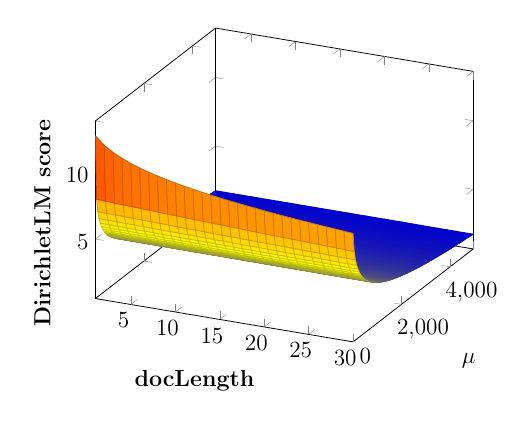
\begin{tikzpicture}[thick,scale=0.7, every node/.style={transform shape}]\begin{axis}[
 %title={},
 %y dir=reverse, 
 %x dir=reverse, 
 ylabel={$\mu$},
 xlabel={docLength},
 zlabel={DirichletLM score},
 every axis/.append style={font=\large\bfseries},
 max space between ticks=25pt
% yticklabels={0k,100k}
 ] 

		\addplot3[surf] coordinates { 
%patch,patch type=biquadratic, shader=faceted,patch refines=3
(1.00,1.00,12.52)(2.00,1.00,11.93)(3.00,1.00,11.52)(4.00,1.00,11.20)(5.00,1.00,10.93)(6.00,1.00,10.71)(7.00,1.00,10.52)(8.00,1.00,10.35)(9.00,1.00,10.20)(10.00,1.00,10.06)(11.00,1.00,9.93)(12.00,1.00,9.82)(13.00,1.00,9.71)(14.00,1.00,9.61)(15.00,1.00,9.52)(16.00,1.00,9.43)(17.00,1.00,9.35)(18.00,1.00,9.27)(19.00,1.00,9.20)(20.00,1.00,9.12)(21.00,1.00,9.06)(22.00,1.00,8.99)(23.00,1.00,8.93)(24.00,1.00,8.87)(25.00,1.00,8.82)(26.00,1.00,8.76)(27.00,1.00,8.71)(28.00,1.00,8.66)(29.00,1.00,8.61)(30.00,1.00,8.56)

(1.00,51.00,7.82)(2.00,51.00,7.80)(3.00,51.00,7.77)(4.00,51.00,7.74)(5.00,51.00,7.72)(6.00,51.00,7.69)(7.00,51.00,7.67)(8.00,51.00,7.64)(9.00,51.00,7.62)(10.00,51.00,7.59)(11.00,51.00,7.57)(12.00,51.00,7.55)(13.00,51.00,7.52)(14.00,51.00,7.50)(15.00,51.00,7.48)(16.00,51.00,7.46)(17.00,51.00,7.44)(18.00,51.00,7.41)(19.00,51.00,7.39)(20.00,51.00,7.37)(21.00,51.00,7.35)(22.00,51.00,7.33)(23.00,51.00,7.31)(24.00,51.00,7.29)(25.00,51.00,7.28)(26.00,51.00,7.26)(27.00,51.00,7.24)(28.00,51.00,7.22)(29.00,51.00,7.20)(30.00,51.00,7.18)

(1.00,101.00,6.86)(2.00,101.00,6.84)(3.00,101.00,6.83)(4.00,101.00,6.82)(5.00,101.00,6.80)(6.00,101.00,6.79)(7.00,101.00,6.77)(8.00,101.00,6.76)(9.00,101.00,6.75)(10.00,101.00,6.73)(11.00,101.00,6.72)(12.00,101.00,6.71)(13.00,101.00,6.70)(14.00,101.00,6.68)(15.00,101.00,6.67)(16.00,101.00,6.66)(17.00,101.00,6.65)(18.00,101.00,6.63)(19.00,101.00,6.62)(20.00,101.00,6.61)(21.00,101.00,6.60)(22.00,101.00,6.59)(23.00,101.00,6.58)(24.00,101.00,6.56)(25.00,101.00,6.55)(26.00,101.00,6.54)(27.00,101.00,6.53)(28.00,101.00,6.52)(29.00,101.00,6.51)(30.00,101.00,6.50)

(1.00,151.00,6.29)(2.00,151.00,6.28)(3.00,151.00,6.27)(4.00,151.00,6.26)(5.00,151.00,6.25)(6.00,151.00,6.24)(7.00,151.00,6.23)(8.00,151.00,6.22)(9.00,151.00,6.21)(10.00,151.00,6.20)(11.00,151.00,6.20)(12.00,151.00,6.19)(13.00,151.00,6.18)(14.00,151.00,6.17)(15.00,151.00,6.16)(16.00,151.00,6.15)(17.00,151.00,6.14)(18.00,151.00,6.13)(19.00,151.00,6.13)(20.00,151.00,6.12)(21.00,151.00,6.11)(22.00,151.00,6.10)(23.00,151.00,6.09)(24.00,151.00,6.08)(25.00,151.00,6.08)(26.00,151.00,6.07)(27.00,151.00,6.06)(28.00,151.00,6.05)(29.00,151.00,6.04)(30.00,151.00,6.04)

(1.00,201.00,5.88)(2.00,201.00,5.88)(3.00,201.00,5.87)(4.00,201.00,5.86)(5.00,201.00,5.85)(6.00,201.00,5.85)(7.00,201.00,5.84)(8.00,201.00,5.83)(9.00,201.00,5.83)(10.00,201.00,5.82)(11.00,201.00,5.81)(12.00,201.00,5.81)(13.00,201.00,5.80)(14.00,201.00,5.79)(15.00,201.00,5.79)(16.00,201.00,5.78)(17.00,201.00,5.77)(18.00,201.00,5.77)(19.00,201.00,5.76)(20.00,201.00,5.75)(21.00,201.00,5.75)(22.00,201.00,5.74)(23.00,201.00,5.73)(24.00,201.00,5.73)(25.00,201.00,5.72)(26.00,201.00,5.71)(27.00,201.00,5.71)(28.00,201.00,5.70)(29.00,201.00,5.70)(30.00,201.00,5.69)

(1.00,251.00,5.57)(2.00,251.00,5.56)(3.00,251.00,5.56)(4.00,251.00,5.55)(5.00,251.00,5.55)(6.00,251.00,5.54)(7.00,251.00,5.54)(8.00,251.00,5.53)(9.00,251.00,5.53)(10.00,251.00,5.52)(11.00,251.00,5.51)(12.00,251.00,5.51)(13.00,251.00,5.50)(14.00,251.00,5.50)(15.00,251.00,5.49)(16.00,251.00,5.49)(17.00,251.00,5.48)(18.00,251.00,5.48)(19.00,251.00,5.47)(20.00,251.00,5.47)(21.00,251.00,5.46)(22.00,251.00,5.45)(23.00,251.00,5.45)(24.00,251.00,5.44)(25.00,251.00,5.44)(26.00,251.00,5.43)(27.00,251.00,5.43)(28.00,251.00,5.42)(29.00,251.00,5.42)(30.00,251.00,5.41)

(1.00,301.00,5.32)(2.00,301.00,5.31)(3.00,301.00,5.31)(4.00,301.00,5.30)(5.00,301.00,5.30)(6.00,301.00,5.29)(7.00,301.00,5.29)(8.00,301.00,5.28)(9.00,301.00,5.28)(10.00,301.00,5.27)(11.00,301.00,5.27)(12.00,301.00,5.26)(13.00,301.00,5.26)(14.00,301.00,5.25)(15.00,301.00,5.25)(16.00,301.00,5.25)(17.00,301.00,5.24)(18.00,301.00,5.24)(19.00,301.00,5.23)(20.00,301.00,5.23)(21.00,301.00,5.22)(22.00,301.00,5.22)(23.00,301.00,5.21)(24.00,301.00,5.21)(25.00,301.00,5.20)(26.00,301.00,5.20)(27.00,301.00,5.20)(28.00,301.00,5.19)(29.00,301.00,5.19)(30.00,301.00,5.18)

(1.00,351.00,5.10)(2.00,351.00,5.10)(3.00,351.00,5.09)(4.00,351.00,5.09)(5.00,351.00,5.08)(6.00,351.00,5.08)(7.00,351.00,5.08)(8.00,351.00,5.07)(9.00,351.00,5.07)(10.00,351.00,5.06)(11.00,351.00,5.06)(12.00,351.00,5.06)(13.00,351.00,5.05)(14.00,351.00,5.05)(15.00,351.00,5.04)(16.00,351.00,5.04)(17.00,351.00,5.04)(18.00,351.00,5.03)(19.00,351.00,5.03)(20.00,351.00,5.02)(21.00,351.00,5.02)(22.00,351.00,5.02)(23.00,351.00,5.01)(24.00,351.00,5.01)(25.00,351.00,5.00)(26.00,351.00,5.00)(27.00,351.00,5.00)(28.00,351.00,4.99)(29.00,351.00,4.99)(30.00,351.00,4.99)

(1.00,401.00,4.91)(2.00,401.00,4.91)(3.00,401.00,4.91)(4.00,401.00,4.90)(5.00,401.00,4.90)(6.00,401.00,4.90)(7.00,401.00,4.89)(8.00,401.00,4.89)(9.00,401.00,4.89)(10.00,401.00,4.88)(11.00,401.00,4.88)(12.00,401.00,4.88)(13.00,401.00,4.87)(14.00,401.00,4.87)(15.00,401.00,4.87)(16.00,401.00,4.86)(17.00,401.00,4.86)(18.00,401.00,4.85)(19.00,401.00,4.85)(20.00,401.00,4.85)(21.00,401.00,4.84)(22.00,401.00,4.84)(23.00,401.00,4.84)(24.00,401.00,4.83)(25.00,401.00,4.83)(26.00,401.00,4.83)(27.00,401.00,4.82)(28.00,401.00,4.82)(29.00,401.00,4.82)(30.00,401.00,4.81)

(1.00,451.00,4.75)(2.00,451.00,4.75)(3.00,451.00,4.74)(4.00,451.00,4.74)(5.00,451.00,4.74)(6.00,451.00,4.74)(7.00,451.00,4.73)(8.00,451.00,4.73)(9.00,451.00,4.73)(10.00,451.00,4.72)(11.00,451.00,4.72)(12.00,451.00,4.72)(13.00,451.00,4.71)(14.00,451.00,4.71)(15.00,451.00,4.71)(16.00,451.00,4.70)(17.00,451.00,4.70)(18.00,451.00,4.70)(19.00,451.00,4.69)(20.00,451.00,4.69)(21.00,451.00,4.69)(22.00,451.00,4.69)(23.00,451.00,4.68)(24.00,451.00,4.68)(25.00,451.00,4.68)(26.00,451.00,4.67)(27.00,451.00,4.67)(28.00,451.00,4.67)(29.00,451.00,4.66)(30.00,451.00,4.66)

(1.00,501.00,4.61)(2.00,501.00,4.60)(3.00,501.00,4.60)(4.00,501.00,4.60)(5.00,501.00,4.59)(6.00,501.00,4.59)(7.00,501.00,4.59)(8.00,501.00,4.59)(9.00,501.00,4.58)(10.00,501.00,4.58)(11.00,501.00,4.58)(12.00,501.00,4.57)(13.00,501.00,4.57)(14.00,501.00,4.57)(15.00,501.00,4.57)(16.00,501.00,4.56)(17.00,501.00,4.56)(18.00,501.00,4.56)(19.00,501.00,4.55)(20.00,501.00,4.55)(21.00,501.00,4.55)(22.00,501.00,4.55)(23.00,501.00,4.54)(24.00,501.00,4.54)(25.00,501.00,4.54)(26.00,501.00,4.54)(27.00,501.00,4.53)(28.00,501.00,4.53)(29.00,501.00,4.53)(30.00,501.00,4.52)

(1.00,551.00,4.47)(2.00,551.00,4.47)(3.00,551.00,4.47)(4.00,551.00,4.47)(5.00,551.00,4.46)(6.00,551.00,4.46)(7.00,551.00,4.46)(8.00,551.00,4.46)(9.00,551.00,4.45)(10.00,551.00,4.45)(11.00,551.00,4.45)(12.00,551.00,4.45)(13.00,551.00,4.44)(14.00,551.00,4.44)(15.00,551.00,4.44)(16.00,551.00,4.44)(17.00,551.00,4.43)(18.00,551.00,4.43)(19.00,551.00,4.43)(20.00,551.00,4.43)(21.00,551.00,4.42)(22.00,551.00,4.42)(23.00,551.00,4.42)(24.00,551.00,4.42)(25.00,551.00,4.41)(26.00,551.00,4.41)(27.00,551.00,4.41)(28.00,551.00,4.41)(29.00,551.00,4.40)(30.00,551.00,4.40)

(1.00,601.00,4.36)(2.00,601.00,4.35)(3.00,601.00,4.35)(4.00,601.00,4.35)(5.00,601.00,4.35)(6.00,601.00,4.34)(7.00,601.00,4.34)(8.00,601.00,4.34)(9.00,601.00,4.34)(10.00,601.00,4.33)(11.00,601.00,4.33)(12.00,601.00,4.33)(13.00,601.00,4.33)(14.00,601.00,4.32)(15.00,601.00,4.32)(16.00,601.00,4.32)(17.00,601.00,4.32)(18.00,601.00,4.32)(19.00,601.00,4.31)(20.00,601.00,4.31)(21.00,601.00,4.31)(22.00,601.00,4.31)(23.00,601.00,4.30)(24.00,601.00,4.30)(25.00,601.00,4.30)(26.00,601.00,4.30)(27.00,601.00,4.29)(28.00,601.00,4.29)(29.00,601.00,4.29)(30.00,601.00,4.29)

(1.00,651.00,4.25)(2.00,651.00,4.24)(3.00,651.00,4.24)(4.00,651.00,4.24)(5.00,651.00,4.24)(6.00,651.00,4.24)(7.00,651.00,4.23)(8.00,651.00,4.23)(9.00,651.00,4.23)(10.00,651.00,4.23)(11.00,651.00,4.22)(12.00,651.00,4.22)(13.00,651.00,4.22)(14.00,651.00,4.22)(15.00,651.00,4.22)(16.00,651.00,4.21)(17.00,651.00,4.21)(18.00,651.00,4.21)(19.00,651.00,4.21)(20.00,651.00,4.20)(21.00,651.00,4.20)(22.00,651.00,4.20)(23.00,651.00,4.20)(24.00,651.00,4.20)(25.00,651.00,4.19)(26.00,651.00,4.19)(27.00,651.00,4.19)(28.00,651.00,4.19)(29.00,651.00,4.19)(30.00,651.00,4.18)

(1.00,701.00,4.15)(2.00,701.00,4.14)(3.00,701.00,4.14)(4.00,701.00,4.14)(5.00,701.00,4.14)(6.00,701.00,4.14)(7.00,701.00,4.13)(8.00,701.00,4.13)(9.00,701.00,4.13)(10.00,701.00,4.13)(11.00,701.00,4.13)(12.00,701.00,4.12)(13.00,701.00,4.12)(14.00,701.00,4.12)(15.00,701.00,4.12)(16.00,701.00,4.11)(17.00,701.00,4.11)(18.00,701.00,4.11)(19.00,701.00,4.11)(20.00,701.00,4.11)(21.00,701.00,4.10)(22.00,701.00,4.10)(23.00,701.00,4.10)(24.00,701.00,4.10)(25.00,701.00,4.10)(26.00,701.00,4.09)(27.00,701.00,4.09)(28.00,701.00,4.09)(29.00,701.00,4.09)(30.00,701.00,4.09)

(1.00,751.00,4.05)(2.00,751.00,4.05)(3.00,751.00,4.05)(4.00,751.00,4.05)(5.00,751.00,4.04)(6.00,751.00,4.04)(7.00,751.00,4.04)(8.00,751.00,4.04)(9.00,751.00,4.04)(10.00,751.00,4.03)(11.00,751.00,4.03)(12.00,751.00,4.03)(13.00,751.00,4.03)(14.00,751.00,4.03)(15.00,751.00,4.03)(16.00,751.00,4.02)(17.00,751.00,4.02)(18.00,751.00,4.02)(19.00,751.00,4.02)(20.00,751.00,4.02)(21.00,751.00,4.01)(22.00,751.00,4.01)(23.00,751.00,4.01)(24.00,751.00,4.01)(25.00,751.00,4.01)(26.00,751.00,4.00)(27.00,751.00,4.00)(28.00,751.00,4.00)(29.00,751.00,4.00)(30.00,751.00,4.00)

(1.00,801.00,3.96)(2.00,801.00,3.96)(3.00,801.00,3.96)(4.00,801.00,3.96)(5.00,801.00,3.96)(6.00,801.00,3.96)(7.00,801.00,3.95)(8.00,801.00,3.95)(9.00,801.00,3.95)(10.00,801.00,3.95)(11.00,801.00,3.95)(12.00,801.00,3.95)(13.00,801.00,3.94)(14.00,801.00,3.94)(15.00,801.00,3.94)(16.00,801.00,3.94)(17.00,801.00,3.94)(18.00,801.00,3.93)(19.00,801.00,3.93)(20.00,801.00,3.93)(21.00,801.00,3.93)(22.00,801.00,3.93)(23.00,801.00,3.93)(24.00,801.00,3.92)(25.00,801.00,3.92)(26.00,801.00,3.92)(27.00,801.00,3.92)(28.00,801.00,3.92)(29.00,801.00,3.92)(30.00,801.00,3.91)

(1.00,851.00,3.88)(2.00,851.00,3.88)(3.00,851.00,3.88)(4.00,851.00,3.88)(5.00,851.00,3.88)(6.00,851.00,3.87)(7.00,851.00,3.87)(8.00,851.00,3.87)(9.00,851.00,3.87)(10.00,851.00,3.87)(11.00,851.00,3.87)(12.00,851.00,3.86)(13.00,851.00,3.86)(14.00,851.00,3.86)(15.00,851.00,3.86)(16.00,851.00,3.86)(17.00,851.00,3.86)(18.00,851.00,3.85)(19.00,851.00,3.85)(20.00,851.00,3.85)(21.00,851.00,3.85)(22.00,851.00,3.85)(23.00,851.00,3.85)(24.00,851.00,3.84)(25.00,851.00,3.84)(26.00,851.00,3.84)(27.00,851.00,3.84)(28.00,851.00,3.84)(29.00,851.00,3.84)(30.00,851.00,3.84)

(1.00,901.00,3.81)(2.00,901.00,3.81)(3.00,901.00,3.80)(4.00,901.00,3.80)(5.00,901.00,3.80)(6.00,901.00,3.80)(7.00,901.00,3.80)(8.00,901.00,3.80)(9.00,901.00,3.79)(10.00,901.00,3.79)(11.00,901.00,3.79)(12.00,901.00,3.79)(13.00,901.00,3.79)(14.00,901.00,3.79)(15.00,901.00,3.78)(16.00,901.00,3.78)(17.00,901.00,3.78)(18.00,901.00,3.78)(19.00,901.00,3.78)(20.00,901.00,3.78)(21.00,901.00,3.78)(22.00,901.00,3.77)(23.00,901.00,3.77)(24.00,901.00,3.77)(25.00,901.00,3.77)(26.00,901.00,3.77)(27.00,901.00,3.77)(28.00,901.00,3.76)(29.00,901.00,3.76)(30.00,901.00,3.76)

(1.00,951.00,3.73)(2.00,951.00,3.73)(3.00,951.00,3.73)(4.00,951.00,3.73)(5.00,951.00,3.73)(6.00,951.00,3.73)(7.00,951.00,3.73)(8.00,951.00,3.72)(9.00,951.00,3.72)(10.00,951.00,3.72)(11.00,951.00,3.72)(12.00,951.00,3.72)(13.00,951.00,3.72)(14.00,951.00,3.72)(15.00,951.00,3.71)(16.00,951.00,3.71)(17.00,951.00,3.71)(18.00,951.00,3.71)(19.00,951.00,3.71)(20.00,951.00,3.71)(21.00,951.00,3.70)(22.00,951.00,3.70)(23.00,951.00,3.70)(24.00,951.00,3.70)(25.00,951.00,3.70)(26.00,951.00,3.70)(27.00,951.00,3.70)(28.00,951.00,3.69)(29.00,951.00,3.69)(30.00,951.00,3.69)

(1.00,1001.00,3.67)(2.00,1001.00,3.67)(3.00,1001.00,3.66)(4.00,1001.00,3.66)(5.00,1001.00,3.66)(6.00,1001.00,3.66)(7.00,1001.00,3.66)(8.00,1001.00,3.66)(9.00,1001.00,3.66)(10.00,1001.00,3.65)(11.00,1001.00,3.65)(12.00,1001.00,3.65)(13.00,1001.00,3.65)(14.00,1001.00,3.65)(15.00,1001.00,3.65)(16.00,1001.00,3.65)(17.00,1001.00,3.64)(18.00,1001.00,3.64)(19.00,1001.00,3.64)(20.00,1001.00,3.64)(21.00,1001.00,3.64)(22.00,1001.00,3.64)(23.00,1001.00,3.64)(24.00,1001.00,3.63)(25.00,1001.00,3.63)(26.00,1001.00,3.63)(27.00,1001.00,3.63)(28.00,1001.00,3.63)(29.00,1001.00,3.63)(30.00,1001.00,3.63)

(1.00,1051.00,3.60)(2.00,1051.00,3.60)(3.00,1051.00,3.60)(4.00,1051.00,3.60)(5.00,1051.00,3.60)(6.00,1051.00,3.60)(7.00,1051.00,3.59)(8.00,1051.00,3.59)(9.00,1051.00,3.59)(10.00,1051.00,3.59)(11.00,1051.00,3.59)(12.00,1051.00,3.59)(13.00,1051.00,3.59)(14.00,1051.00,3.58)(15.00,1051.00,3.58)(16.00,1051.00,3.58)(17.00,1051.00,3.58)(18.00,1051.00,3.58)(19.00,1051.00,3.58)(20.00,1051.00,3.58)(21.00,1051.00,3.57)(22.00,1051.00,3.57)(23.00,1051.00,3.57)(24.00,1051.00,3.57)(25.00,1051.00,3.57)(26.00,1051.00,3.57)(27.00,1051.00,3.57)(28.00,1051.00,3.57)(29.00,1051.00,3.56)(30.00,1051.00,3.56)

(1.00,1101.00,3.54)(2.00,1101.00,3.54)(3.00,1101.00,3.54)(4.00,1101.00,3.54)(5.00,1101.00,3.54)(6.00,1101.00,3.53)(7.00,1101.00,3.53)(8.00,1101.00,3.53)(9.00,1101.00,3.53)(10.00,1101.00,3.53)(11.00,1101.00,3.53)(12.00,1101.00,3.53)(13.00,1101.00,3.52)(14.00,1101.00,3.52)(15.00,1101.00,3.52)(16.00,1101.00,3.52)(17.00,1101.00,3.52)(18.00,1101.00,3.52)(19.00,1101.00,3.52)(20.00,1101.00,3.52)(21.00,1101.00,3.51)(22.00,1101.00,3.51)(23.00,1101.00,3.51)(24.00,1101.00,3.51)(25.00,1101.00,3.51)(26.00,1101.00,3.51)(27.00,1101.00,3.51)(28.00,1101.00,3.51)(29.00,1101.00,3.50)(30.00,1101.00,3.50)

(1.00,1151.00,3.48)(2.00,1151.00,3.48)(3.00,1151.00,3.48)(4.00,1151.00,3.48)(5.00,1151.00,3.48)(6.00,1151.00,3.48)(7.00,1151.00,3.47)(8.00,1151.00,3.47)(9.00,1151.00,3.47)(10.00,1151.00,3.47)(11.00,1151.00,3.47)(12.00,1151.00,3.47)(13.00,1151.00,3.47)(14.00,1151.00,3.47)(15.00,1151.00,3.46)(16.00,1151.00,3.46)(17.00,1151.00,3.46)(18.00,1151.00,3.46)(19.00,1151.00,3.46)(20.00,1151.00,3.46)(21.00,1151.00,3.46)(22.00,1151.00,3.46)(23.00,1151.00,3.45)(24.00,1151.00,3.45)(25.00,1151.00,3.45)(26.00,1151.00,3.45)(27.00,1151.00,3.45)(28.00,1151.00,3.45)(29.00,1151.00,3.45)(30.00,1151.00,3.45)

(1.00,1201.00,3.43)(2.00,1201.00,3.43)(3.00,1201.00,3.42)(4.00,1201.00,3.42)(5.00,1201.00,3.42)(6.00,1201.00,3.42)(7.00,1201.00,3.42)(8.00,1201.00,3.42)(9.00,1201.00,3.42)(10.00,1201.00,3.42)(11.00,1201.00,3.41)(12.00,1201.00,3.41)(13.00,1201.00,3.41)(14.00,1201.00,3.41)(15.00,1201.00,3.41)(16.00,1201.00,3.41)(17.00,1201.00,3.41)(18.00,1201.00,3.41)(19.00,1201.00,3.40)(20.00,1201.00,3.40)(21.00,1201.00,3.40)(22.00,1201.00,3.40)(23.00,1201.00,3.40)(24.00,1201.00,3.40)(25.00,1201.00,3.40)(26.00,1201.00,3.40)(27.00,1201.00,3.40)(28.00,1201.00,3.39)(29.00,1201.00,3.39)(30.00,1201.00,3.39)

(1.00,1251.00,3.37)(2.00,1251.00,3.37)(3.00,1251.00,3.37)(4.00,1251.00,3.37)(5.00,1251.00,3.37)(6.00,1251.00,3.37)(7.00,1251.00,3.37)(8.00,1251.00,3.37)(9.00,1251.00,3.36)(10.00,1251.00,3.36)(11.00,1251.00,3.36)(12.00,1251.00,3.36)(13.00,1251.00,3.36)(14.00,1251.00,3.36)(15.00,1251.00,3.36)(16.00,1251.00,3.36)(17.00,1251.00,3.35)(18.00,1251.00,3.35)(19.00,1251.00,3.35)(20.00,1251.00,3.35)(21.00,1251.00,3.35)(22.00,1251.00,3.35)(23.00,1251.00,3.35)(24.00,1251.00,3.35)(25.00,1251.00,3.35)(26.00,1251.00,3.34)(27.00,1251.00,3.34)(28.00,1251.00,3.34)(29.00,1251.00,3.34)(30.00,1251.00,3.34)

(1.00,1301.00,3.32)(2.00,1301.00,3.32)(3.00,1301.00,3.32)(4.00,1301.00,3.32)(5.00,1301.00,3.32)(6.00,1301.00,3.32)(7.00,1301.00,3.32)(8.00,1301.00,3.31)(9.00,1301.00,3.31)(10.00,1301.00,3.31)(11.00,1301.00,3.31)(12.00,1301.00,3.31)(13.00,1301.00,3.31)(14.00,1301.00,3.31)(15.00,1301.00,3.31)(16.00,1301.00,3.31)(17.00,1301.00,3.30)(18.00,1301.00,3.30)(19.00,1301.00,3.30)(20.00,1301.00,3.30)(21.00,1301.00,3.30)(22.00,1301.00,3.30)(23.00,1301.00,3.30)(24.00,1301.00,3.30)(25.00,1301.00,3.30)(26.00,1301.00,3.29)(27.00,1301.00,3.29)(28.00,1301.00,3.29)(29.00,1301.00,3.29)(30.00,1301.00,3.29)

(1.00,1351.00,3.27)(2.00,1351.00,3.27)(3.00,1351.00,3.27)(4.00,1351.00,3.27)(5.00,1351.00,3.27)(6.00,1351.00,3.27)(7.00,1351.00,3.27)(8.00,1351.00,3.27)(9.00,1351.00,3.26)(10.00,1351.00,3.26)(11.00,1351.00,3.26)(12.00,1351.00,3.26)(13.00,1351.00,3.26)(14.00,1351.00,3.26)(15.00,1351.00,3.26)(16.00,1351.00,3.26)(17.00,1351.00,3.26)(18.00,1351.00,3.26)(19.00,1351.00,3.25)(20.00,1351.00,3.25)(21.00,1351.00,3.25)(22.00,1351.00,3.25)(23.00,1351.00,3.25)(24.00,1351.00,3.25)(25.00,1351.00,3.25)(26.00,1351.00,3.25)(27.00,1351.00,3.25)(28.00,1351.00,3.24)(29.00,1351.00,3.24)(30.00,1351.00,3.24)

(1.00,1401.00,3.23)(2.00,1401.00,3.23)(3.00,1401.00,3.22)(4.00,1401.00,3.22)(5.00,1401.00,3.22)(6.00,1401.00,3.22)(7.00,1401.00,3.22)(8.00,1401.00,3.22)(9.00,1401.00,3.22)(10.00,1401.00,3.22)(11.00,1401.00,3.22)(12.00,1401.00,3.22)(13.00,1401.00,3.21)(14.00,1401.00,3.21)(15.00,1401.00,3.21)(16.00,1401.00,3.21)(17.00,1401.00,3.21)(18.00,1401.00,3.21)(19.00,1401.00,3.21)(20.00,1401.00,3.21)(21.00,1401.00,3.21)(22.00,1401.00,3.21)(23.00,1401.00,3.20)(24.00,1401.00,3.20)(25.00,1401.00,3.20)(26.00,1401.00,3.20)(27.00,1401.00,3.20)(28.00,1401.00,3.20)(29.00,1401.00,3.20)(30.00,1401.00,3.20)

(1.00,1451.00,3.18)(2.00,1451.00,3.18)(3.00,1451.00,3.18)(4.00,1451.00,3.18)(5.00,1451.00,3.18)(6.00,1451.00,3.18)(7.00,1451.00,3.18)(8.00,1451.00,3.17)(9.00,1451.00,3.17)(10.00,1451.00,3.17)(11.00,1451.00,3.17)(12.00,1451.00,3.17)(13.00,1451.00,3.17)(14.00,1451.00,3.17)(15.00,1451.00,3.17)(16.00,1451.00,3.17)(17.00,1451.00,3.17)(18.00,1451.00,3.16)(19.00,1451.00,3.16)(20.00,1451.00,3.16)(21.00,1451.00,3.16)(22.00,1451.00,3.16)(23.00,1451.00,3.16)(24.00,1451.00,3.16)(25.00,1451.00,3.16)(26.00,1451.00,3.16)(27.00,1451.00,3.16)(28.00,1451.00,3.15)(29.00,1451.00,3.15)(30.00,1451.00,3.15)

(1.00,1501.00,3.14)(2.00,1501.00,3.14)(3.00,1501.00,3.14)(4.00,1501.00,3.14)(5.00,1501.00,3.13)(6.00,1501.00,3.13)(7.00,1501.00,3.13)(8.00,1501.00,3.13)(9.00,1501.00,3.13)(10.00,1501.00,3.13)(11.00,1501.00,3.13)(12.00,1501.00,3.13)(13.00,1501.00,3.13)(14.00,1501.00,3.13)(15.00,1501.00,3.12)(16.00,1501.00,3.12)(17.00,1501.00,3.12)(18.00,1501.00,3.12)(19.00,1501.00,3.12)(20.00,1501.00,3.12)(21.00,1501.00,3.12)(22.00,1501.00,3.12)(23.00,1501.00,3.12)(24.00,1501.00,3.12)(25.00,1501.00,3.12)(26.00,1501.00,3.11)(27.00,1501.00,3.11)(28.00,1501.00,3.11)(29.00,1501.00,3.11)(30.00,1501.00,3.11)

(1.00,1551.00,3.10)(2.00,1551.00,3.10)(3.00,1551.00,3.09)(4.00,1551.00,3.09)(5.00,1551.00,3.09)(6.00,1551.00,3.09)(7.00,1551.00,3.09)(8.00,1551.00,3.09)(9.00,1551.00,3.09)(10.00,1551.00,3.09)(11.00,1551.00,3.09)(12.00,1551.00,3.09)(13.00,1551.00,3.09)(14.00,1551.00,3.08)(15.00,1551.00,3.08)(16.00,1551.00,3.08)(17.00,1551.00,3.08)(18.00,1551.00,3.08)(19.00,1551.00,3.08)(20.00,1551.00,3.08)(21.00,1551.00,3.08)(22.00,1551.00,3.08)(23.00,1551.00,3.08)(24.00,1551.00,3.08)(25.00,1551.00,3.07)(26.00,1551.00,3.07)(27.00,1551.00,3.07)(28.00,1551.00,3.07)(29.00,1551.00,3.07)(30.00,1551.00,3.07)

(1.00,1601.00,3.06)(2.00,1601.00,3.06)(3.00,1601.00,3.05)(4.00,1601.00,3.05)(5.00,1601.00,3.05)(6.00,1601.00,3.05)(7.00,1601.00,3.05)(8.00,1601.00,3.05)(9.00,1601.00,3.05)(10.00,1601.00,3.05)(11.00,1601.00,3.05)(12.00,1601.00,3.05)(13.00,1601.00,3.05)(14.00,1601.00,3.04)(15.00,1601.00,3.04)(16.00,1601.00,3.04)(17.00,1601.00,3.04)(18.00,1601.00,3.04)(19.00,1601.00,3.04)(20.00,1601.00,3.04)(21.00,1601.00,3.04)(22.00,1601.00,3.04)(23.00,1601.00,3.04)(24.00,1601.00,3.04)(25.00,1601.00,3.03)(26.00,1601.00,3.03)(27.00,1601.00,3.03)(28.00,1601.00,3.03)(29.00,1601.00,3.03)(30.00,1601.00,3.03)

(1.00,1651.00,3.02)(2.00,1651.00,3.02)(3.00,1651.00,3.02)(4.00,1651.00,3.01)(5.00,1651.00,3.01)(6.00,1651.00,3.01)(7.00,1651.00,3.01)(8.00,1651.00,3.01)(9.00,1651.00,3.01)(10.00,1651.00,3.01)(11.00,1651.00,3.01)(12.00,1651.00,3.01)(13.00,1651.00,3.01)(14.00,1651.00,3.01)(15.00,1651.00,3.00)(16.00,1651.00,3.00)(17.00,1651.00,3.00)(18.00,1651.00,3.00)(19.00,1651.00,3.00)(20.00,1651.00,3.00)(21.00,1651.00,3.00)(22.00,1651.00,3.00)(23.00,1651.00,3.00)(24.00,1651.00,3.00)(25.00,1651.00,3.00)(26.00,1651.00,3.00)(27.00,1651.00,2.99)(28.00,1651.00,2.99)(29.00,1651.00,2.99)(30.00,1651.00,2.99)

(1.00,1701.00,2.98)(2.00,1701.00,2.98)(3.00,1701.00,2.98)(4.00,1701.00,2.98)(5.00,1701.00,2.98)(6.00,1701.00,2.98)(7.00,1701.00,2.97)(8.00,1701.00,2.97)(9.00,1701.00,2.97)(10.00,1701.00,2.97)(11.00,1701.00,2.97)(12.00,1701.00,2.97)(13.00,1701.00,2.97)(14.00,1701.00,2.97)(15.00,1701.00,2.97)(16.00,1701.00,2.97)(17.00,1701.00,2.97)(18.00,1701.00,2.97)(19.00,1701.00,2.96)(20.00,1701.00,2.96)(21.00,1701.00,2.96)(22.00,1701.00,2.96)(23.00,1701.00,2.96)(24.00,1701.00,2.96)(25.00,1701.00,2.96)(26.00,1701.00,2.96)(27.00,1701.00,2.96)(28.00,1701.00,2.96)(29.00,1701.00,2.96)(30.00,1701.00,2.96)

(1.00,1751.00,2.94)(2.00,1751.00,2.94)(3.00,1751.00,2.94)(4.00,1751.00,2.94)(5.00,1751.00,2.94)(6.00,1751.00,2.94)(7.00,1751.00,2.94)(8.00,1751.00,2.94)(9.00,1751.00,2.94)(10.00,1751.00,2.94)(11.00,1751.00,2.93)(12.00,1751.00,2.93)(13.00,1751.00,2.93)(14.00,1751.00,2.93)(15.00,1751.00,2.93)(16.00,1751.00,2.93)(17.00,1751.00,2.93)(18.00,1751.00,2.93)(19.00,1751.00,2.93)(20.00,1751.00,2.93)(21.00,1751.00,2.93)(22.00,1751.00,2.93)(23.00,1751.00,2.93)(24.00,1751.00,2.92)(25.00,1751.00,2.92)(26.00,1751.00,2.92)(27.00,1751.00,2.92)(28.00,1751.00,2.92)(29.00,1751.00,2.92)(30.00,1751.00,2.92)

(1.00,1801.00,2.91)(2.00,1801.00,2.91)(3.00,1801.00,2.91)(4.00,1801.00,2.91)(5.00,1801.00,2.90)(6.00,1801.00,2.90)(7.00,1801.00,2.90)(8.00,1801.00,2.90)(9.00,1801.00,2.90)(10.00,1801.00,2.90)(11.00,1801.00,2.90)(12.00,1801.00,2.90)(13.00,1801.00,2.90)(14.00,1801.00,2.90)(15.00,1801.00,2.90)(16.00,1801.00,2.90)(17.00,1801.00,2.90)(18.00,1801.00,2.89)(19.00,1801.00,2.89)(20.00,1801.00,2.89)(21.00,1801.00,2.89)(22.00,1801.00,2.89)(23.00,1801.00,2.89)(24.00,1801.00,2.89)(25.00,1801.00,2.89)(26.00,1801.00,2.89)(27.00,1801.00,2.89)(28.00,1801.00,2.89)(29.00,1801.00,2.89)(30.00,1801.00,2.88)

(1.00,1851.00,2.87)(2.00,1851.00,2.87)(3.00,1851.00,2.87)(4.00,1851.00,2.87)(5.00,1851.00,2.87)(6.00,1851.00,2.87)(7.00,1851.00,2.87)(8.00,1851.00,2.87)(9.00,1851.00,2.87)(10.00,1851.00,2.87)(11.00,1851.00,2.87)(12.00,1851.00,2.87)(13.00,1851.00,2.86)(14.00,1851.00,2.86)(15.00,1851.00,2.86)(16.00,1851.00,2.86)(17.00,1851.00,2.86)(18.00,1851.00,2.86)(19.00,1851.00,2.86)(20.00,1851.00,2.86)(21.00,1851.00,2.86)(22.00,1851.00,2.86)(23.00,1851.00,2.86)(24.00,1851.00,2.86)(25.00,1851.00,2.86)(26.00,1851.00,2.85)(27.00,1851.00,2.85)(28.00,1851.00,2.85)(29.00,1851.00,2.85)(30.00,1851.00,2.85)

(1.00,1901.00,2.84)(2.00,1901.00,2.84)(3.00,1901.00,2.84)(4.00,1901.00,2.84)(5.00,1901.00,2.84)(6.00,1901.00,2.84)(7.00,1901.00,2.84)(8.00,1901.00,2.84)(9.00,1901.00,2.83)(10.00,1901.00,2.83)(11.00,1901.00,2.83)(12.00,1901.00,2.83)(13.00,1901.00,2.83)(14.00,1901.00,2.83)(15.00,1901.00,2.83)(16.00,1901.00,2.83)(17.00,1901.00,2.83)(18.00,1901.00,2.83)(19.00,1901.00,2.83)(20.00,1901.00,2.83)(21.00,1901.00,2.83)(22.00,1901.00,2.82)(23.00,1901.00,2.82)(24.00,1901.00,2.82)(25.00,1901.00,2.82)(26.00,1901.00,2.82)(27.00,1901.00,2.82)(28.00,1901.00,2.82)(29.00,1901.00,2.82)(30.00,1901.00,2.82)

(1.00,1951.00,2.81)(2.00,1951.00,2.81)(3.00,1951.00,2.81)(4.00,1951.00,2.81)(5.00,1951.00,2.81)(6.00,1951.00,2.80)(7.00,1951.00,2.80)(8.00,1951.00,2.80)(9.00,1951.00,2.80)(10.00,1951.00,2.80)(11.00,1951.00,2.80)(12.00,1951.00,2.80)(13.00,1951.00,2.80)(14.00,1951.00,2.80)(15.00,1951.00,2.80)(16.00,1951.00,2.80)(17.00,1951.00,2.80)(18.00,1951.00,2.80)(19.00,1951.00,2.80)(20.00,1951.00,2.79)(21.00,1951.00,2.79)(22.00,1951.00,2.79)(23.00,1951.00,2.79)(24.00,1951.00,2.79)(25.00,1951.00,2.79)(26.00,1951.00,2.79)(27.00,1951.00,2.79)(28.00,1951.00,2.79)(29.00,1951.00,2.79)(30.00,1951.00,2.79)

(1.00,2001.00,2.78)(2.00,2001.00,2.78)(3.00,2001.00,2.78)(4.00,2001.00,2.77)(5.00,2001.00,2.77)(6.00,2001.00,2.77)(7.00,2001.00,2.77)(8.00,2001.00,2.77)(9.00,2001.00,2.77)(10.00,2001.00,2.77)(11.00,2001.00,2.77)(12.00,2001.00,2.77)(13.00,2001.00,2.77)(14.00,2001.00,2.77)(15.00,2001.00,2.77)(16.00,2001.00,2.77)(17.00,2001.00,2.77)(18.00,2001.00,2.76)(19.00,2001.00,2.76)(20.00,2001.00,2.76)(21.00,2001.00,2.76)(22.00,2001.00,2.76)(23.00,2001.00,2.76)(24.00,2001.00,2.76)(25.00,2001.00,2.76)(26.00,2001.00,2.76)(27.00,2001.00,2.76)(28.00,2001.00,2.76)(29.00,2001.00,2.76)(30.00,2001.00,2.76)

(1.00,2051.00,2.75)(2.00,2051.00,2.75)(3.00,2051.00,2.75)(4.00,2051.00,2.74)(5.00,2051.00,2.74)(6.00,2051.00,2.74)(7.00,2051.00,2.74)(8.00,2051.00,2.74)(9.00,2051.00,2.74)(10.00,2051.00,2.74)(11.00,2051.00,2.74)(12.00,2051.00,2.74)(13.00,2051.00,2.74)(14.00,2051.00,2.74)(15.00,2051.00,2.74)(16.00,2051.00,2.74)(17.00,2051.00,2.74)(18.00,2051.00,2.73)(19.00,2051.00,2.73)(20.00,2051.00,2.73)(21.00,2051.00,2.73)(22.00,2051.00,2.73)(23.00,2051.00,2.73)(24.00,2051.00,2.73)(25.00,2051.00,2.73)(26.00,2051.00,2.73)(27.00,2051.00,2.73)(28.00,2051.00,2.73)(29.00,2051.00,2.73)(30.00,2051.00,2.73)

(1.00,2101.00,2.72)(2.00,2101.00,2.72)(3.00,2101.00,2.72)(4.00,2101.00,2.72)(5.00,2101.00,2.71)(6.00,2101.00,2.71)(7.00,2101.00,2.71)(8.00,2101.00,2.71)(9.00,2101.00,2.71)(10.00,2101.00,2.71)(11.00,2101.00,2.71)(12.00,2101.00,2.71)(13.00,2101.00,2.71)(14.00,2101.00,2.71)(15.00,2101.00,2.71)(16.00,2101.00,2.71)(17.00,2101.00,2.71)(18.00,2101.00,2.71)(19.00,2101.00,2.70)(20.00,2101.00,2.70)(21.00,2101.00,2.70)(22.00,2101.00,2.70)(23.00,2101.00,2.70)(24.00,2101.00,2.70)(25.00,2101.00,2.70)(26.00,2101.00,2.70)(27.00,2101.00,2.70)(28.00,2101.00,2.70)(29.00,2101.00,2.70)(30.00,2101.00,2.70)

(1.00,2151.00,2.69)(2.00,2151.00,2.69)(3.00,2151.00,2.69)(4.00,2151.00,2.69)(5.00,2151.00,2.69)(6.00,2151.00,2.69)(7.00,2151.00,2.68)(8.00,2151.00,2.68)(9.00,2151.00,2.68)(10.00,2151.00,2.68)(11.00,2151.00,2.68)(12.00,2151.00,2.68)(13.00,2151.00,2.68)(14.00,2151.00,2.68)(15.00,2151.00,2.68)(16.00,2151.00,2.68)(17.00,2151.00,2.68)(18.00,2151.00,2.68)(19.00,2151.00,2.68)(20.00,2151.00,2.68)(21.00,2151.00,2.68)(22.00,2151.00,2.67)(23.00,2151.00,2.67)(24.00,2151.00,2.67)(25.00,2151.00,2.67)(26.00,2151.00,2.67)(27.00,2151.00,2.67)(28.00,2151.00,2.67)(29.00,2151.00,2.67)(30.00,2151.00,2.67)

(1.00,2201.00,2.66)(2.00,2201.00,2.66)(3.00,2201.00,2.66)(4.00,2201.00,2.66)(5.00,2201.00,2.66)(6.00,2201.00,2.66)(7.00,2201.00,2.66)(8.00,2201.00,2.66)(9.00,2201.00,2.66)(10.00,2201.00,2.65)(11.00,2201.00,2.65)(12.00,2201.00,2.65)(13.00,2201.00,2.65)(14.00,2201.00,2.65)(15.00,2201.00,2.65)(16.00,2201.00,2.65)(17.00,2201.00,2.65)(18.00,2201.00,2.65)(19.00,2201.00,2.65)(20.00,2201.00,2.65)(21.00,2201.00,2.65)(22.00,2201.00,2.65)(23.00,2201.00,2.65)(24.00,2201.00,2.65)(25.00,2201.00,2.64)(26.00,2201.00,2.64)(27.00,2201.00,2.64)(28.00,2201.00,2.64)(29.00,2201.00,2.64)(30.00,2201.00,2.64)

(1.00,2251.00,2.63)(2.00,2251.00,2.63)(3.00,2251.00,2.63)(4.00,2251.00,2.63)(5.00,2251.00,2.63)(6.00,2251.00,2.63)(7.00,2251.00,2.63)(8.00,2251.00,2.63)(9.00,2251.00,2.63)(10.00,2251.00,2.63)(11.00,2251.00,2.63)(12.00,2251.00,2.63)(13.00,2251.00,2.63)(14.00,2251.00,2.63)(15.00,2251.00,2.62)(16.00,2251.00,2.62)(17.00,2251.00,2.62)(18.00,2251.00,2.62)(19.00,2251.00,2.62)(20.00,2251.00,2.62)(21.00,2251.00,2.62)(22.00,2251.00,2.62)(23.00,2251.00,2.62)(24.00,2251.00,2.62)(25.00,2251.00,2.62)(26.00,2251.00,2.62)(27.00,2251.00,2.62)(28.00,2251.00,2.62)(29.00,2251.00,2.62)(30.00,2251.00,2.61)

(1.00,2301.00,2.61)(2.00,2301.00,2.61)(3.00,2301.00,2.61)(4.00,2301.00,2.60)(5.00,2301.00,2.60)(6.00,2301.00,2.60)(7.00,2301.00,2.60)(8.00,2301.00,2.60)(9.00,2301.00,2.60)(10.00,2301.00,2.60)(11.00,2301.00,2.60)(12.00,2301.00,2.60)(13.00,2301.00,2.60)(14.00,2301.00,2.60)(15.00,2301.00,2.60)(16.00,2301.00,2.60)(17.00,2301.00,2.60)(18.00,2301.00,2.60)(19.00,2301.00,2.60)(20.00,2301.00,2.59)(21.00,2301.00,2.59)(22.00,2301.00,2.59)(23.00,2301.00,2.59)(24.00,2301.00,2.59)(25.00,2301.00,2.59)(26.00,2301.00,2.59)(27.00,2301.00,2.59)(28.00,2301.00,2.59)(29.00,2301.00,2.59)(30.00,2301.00,2.59)

(1.00,2351.00,2.58)(2.00,2351.00,2.58)(3.00,2351.00,2.58)(4.00,2351.00,2.58)(5.00,2351.00,2.58)(6.00,2351.00,2.58)(7.00,2351.00,2.58)(8.00,2351.00,2.58)(9.00,2351.00,2.58)(10.00,2351.00,2.58)(11.00,2351.00,2.57)(12.00,2351.00,2.57)(13.00,2351.00,2.57)(14.00,2351.00,2.57)(15.00,2351.00,2.57)(16.00,2351.00,2.57)(17.00,2351.00,2.57)(18.00,2351.00,2.57)(19.00,2351.00,2.57)(20.00,2351.00,2.57)(21.00,2351.00,2.57)(22.00,2351.00,2.57)(23.00,2351.00,2.57)(24.00,2351.00,2.57)(25.00,2351.00,2.57)(26.00,2351.00,2.57)(27.00,2351.00,2.57)(28.00,2351.00,2.56)(29.00,2351.00,2.56)(30.00,2351.00,2.56)

(1.00,2401.00,2.56)(2.00,2401.00,2.56)(3.00,2401.00,2.55)(4.00,2401.00,2.55)(5.00,2401.00,2.55)(6.00,2401.00,2.55)(7.00,2401.00,2.55)(8.00,2401.00,2.55)(9.00,2401.00,2.55)(10.00,2401.00,2.55)(11.00,2401.00,2.55)(12.00,2401.00,2.55)(13.00,2401.00,2.55)(14.00,2401.00,2.55)(15.00,2401.00,2.55)(16.00,2401.00,2.55)(17.00,2401.00,2.55)(18.00,2401.00,2.55)(19.00,2401.00,2.54)(20.00,2401.00,2.54)(21.00,2401.00,2.54)(22.00,2401.00,2.54)(23.00,2401.00,2.54)(24.00,2401.00,2.54)(25.00,2401.00,2.54)(26.00,2401.00,2.54)(27.00,2401.00,2.54)(28.00,2401.00,2.54)(29.00,2401.00,2.54)(30.00,2401.00,2.54)

(1.00,2451.00,2.53)(2.00,2451.00,2.53)(3.00,2451.00,2.53)(4.00,2451.00,2.53)(5.00,2451.00,2.53)(6.00,2451.00,2.53)(7.00,2451.00,2.53)(8.00,2451.00,2.53)(9.00,2451.00,2.53)(10.00,2451.00,2.53)(11.00,2451.00,2.53)(12.00,2451.00,2.52)(13.00,2451.00,2.52)(14.00,2451.00,2.52)(15.00,2451.00,2.52)(16.00,2451.00,2.52)(17.00,2451.00,2.52)(18.00,2451.00,2.52)(19.00,2451.00,2.52)(20.00,2451.00,2.52)(21.00,2451.00,2.52)(22.00,2451.00,2.52)(23.00,2451.00,2.52)(24.00,2451.00,2.52)(25.00,2451.00,2.52)(26.00,2451.00,2.52)(27.00,2451.00,2.52)(28.00,2451.00,2.52)(29.00,2451.00,2.51)(30.00,2451.00,2.51)

(1.00,2501.00,2.51)(2.00,2501.00,2.51)(3.00,2501.00,2.51)(4.00,2501.00,2.51)(5.00,2501.00,2.50)(6.00,2501.00,2.50)(7.00,2501.00,2.50)(8.00,2501.00,2.50)(9.00,2501.00,2.50)(10.00,2501.00,2.50)(11.00,2501.00,2.50)(12.00,2501.00,2.50)(13.00,2501.00,2.50)(14.00,2501.00,2.50)(15.00,2501.00,2.50)(16.00,2501.00,2.50)(17.00,2501.00,2.50)(18.00,2501.00,2.50)(19.00,2501.00,2.50)(20.00,2501.00,2.50)(21.00,2501.00,2.50)(22.00,2501.00,2.50)(23.00,2501.00,2.49)(24.00,2501.00,2.49)(25.00,2501.00,2.49)(26.00,2501.00,2.49)(27.00,2501.00,2.49)(28.00,2501.00,2.49)(29.00,2501.00,2.49)(30.00,2501.00,2.49)

(1.00,2551.00,2.48)(2.00,2551.00,2.48)(3.00,2551.00,2.48)(4.00,2551.00,2.48)(5.00,2551.00,2.48)(6.00,2551.00,2.48)(7.00,2551.00,2.48)(8.00,2551.00,2.48)(9.00,2551.00,2.48)(10.00,2551.00,2.48)(11.00,2551.00,2.48)(12.00,2551.00,2.48)(13.00,2551.00,2.48)(14.00,2551.00,2.48)(15.00,2551.00,2.48)(16.00,2551.00,2.48)(17.00,2551.00,2.47)(18.00,2551.00,2.47)(19.00,2551.00,2.47)(20.00,2551.00,2.47)(21.00,2551.00,2.47)(22.00,2551.00,2.47)(23.00,2551.00,2.47)(24.00,2551.00,2.47)(25.00,2551.00,2.47)(26.00,2551.00,2.47)(27.00,2551.00,2.47)(28.00,2551.00,2.47)(29.00,2551.00,2.47)(30.00,2551.00,2.47)

(1.00,2601.00,2.46)(2.00,2601.00,2.46)(3.00,2601.00,2.46)(4.00,2601.00,2.46)(5.00,2601.00,2.46)(6.00,2601.00,2.46)(7.00,2601.00,2.46)(8.00,2601.00,2.46)(9.00,2601.00,2.46)(10.00,2601.00,2.46)(11.00,2601.00,2.46)(12.00,2601.00,2.45)(13.00,2601.00,2.45)(14.00,2601.00,2.45)(15.00,2601.00,2.45)(16.00,2601.00,2.45)(17.00,2601.00,2.45)(18.00,2601.00,2.45)(19.00,2601.00,2.45)(20.00,2601.00,2.45)(21.00,2601.00,2.45)(22.00,2601.00,2.45)(23.00,2601.00,2.45)(24.00,2601.00,2.45)(25.00,2601.00,2.45)(26.00,2601.00,2.45)(27.00,2601.00,2.45)(28.00,2601.00,2.45)(29.00,2601.00,2.45)(30.00,2601.00,2.44)

(1.00,2651.00,2.44)(2.00,2651.00,2.44)(3.00,2651.00,2.44)(4.00,2651.00,2.44)(5.00,2651.00,2.44)(6.00,2651.00,2.44)(7.00,2651.00,2.43)(8.00,2651.00,2.43)(9.00,2651.00,2.43)(10.00,2651.00,2.43)(11.00,2651.00,2.43)(12.00,2651.00,2.43)(13.00,2651.00,2.43)(14.00,2651.00,2.43)(15.00,2651.00,2.43)(16.00,2651.00,2.43)(17.00,2651.00,2.43)(18.00,2651.00,2.43)(19.00,2651.00,2.43)(20.00,2651.00,2.43)(21.00,2651.00,2.43)(22.00,2651.00,2.43)(23.00,2651.00,2.43)(24.00,2651.00,2.43)(25.00,2651.00,2.43)(26.00,2651.00,2.42)(27.00,2651.00,2.42)(28.00,2651.00,2.42)(29.00,2651.00,2.42)(30.00,2651.00,2.42)

(1.00,2701.00,2.42)(2.00,2701.00,2.42)(3.00,2701.00,2.42)(4.00,2701.00,2.41)(5.00,2701.00,2.41)(6.00,2701.00,2.41)(7.00,2701.00,2.41)(8.00,2701.00,2.41)(9.00,2701.00,2.41)(10.00,2701.00,2.41)(11.00,2701.00,2.41)(12.00,2701.00,2.41)(13.00,2701.00,2.41)(14.00,2701.00,2.41)(15.00,2701.00,2.41)(16.00,2701.00,2.41)(17.00,2701.00,2.41)(18.00,2701.00,2.41)(19.00,2701.00,2.41)(20.00,2701.00,2.41)(21.00,2701.00,2.41)(22.00,2701.00,2.41)(23.00,2701.00,2.40)(24.00,2701.00,2.40)(25.00,2701.00,2.40)(26.00,2701.00,2.40)(27.00,2701.00,2.40)(28.00,2701.00,2.40)(29.00,2701.00,2.40)(30.00,2701.00,2.40)

(1.00,2751.00,2.39)(2.00,2751.00,2.39)(3.00,2751.00,2.39)(4.00,2751.00,2.39)(5.00,2751.00,2.39)(6.00,2751.00,2.39)(7.00,2751.00,2.39)(8.00,2751.00,2.39)(9.00,2751.00,2.39)(10.00,2751.00,2.39)(11.00,2751.00,2.39)(12.00,2751.00,2.39)(13.00,2751.00,2.39)(14.00,2751.00,2.39)(15.00,2751.00,2.39)(16.00,2751.00,2.39)(17.00,2751.00,2.39)(18.00,2751.00,2.39)(19.00,2751.00,2.39)(20.00,2751.00,2.38)(21.00,2751.00,2.38)(22.00,2751.00,2.38)(23.00,2751.00,2.38)(24.00,2751.00,2.38)(25.00,2751.00,2.38)(26.00,2751.00,2.38)(27.00,2751.00,2.38)(28.00,2751.00,2.38)(29.00,2751.00,2.38)(30.00,2751.00,2.38)

(1.00,2801.00,2.37)(2.00,2801.00,2.37)(3.00,2801.00,2.37)(4.00,2801.00,2.37)(5.00,2801.00,2.37)(6.00,2801.00,2.37)(7.00,2801.00,2.37)(8.00,2801.00,2.37)(9.00,2801.00,2.37)(10.00,2801.00,2.37)(11.00,2801.00,2.37)(12.00,2801.00,2.37)(13.00,2801.00,2.37)(14.00,2801.00,2.37)(15.00,2801.00,2.37)(16.00,2801.00,2.37)(17.00,2801.00,2.37)(18.00,2801.00,2.37)(19.00,2801.00,2.36)(20.00,2801.00,2.36)(21.00,2801.00,2.36)(22.00,2801.00,2.36)(23.00,2801.00,2.36)(24.00,2801.00,2.36)(25.00,2801.00,2.36)(26.00,2801.00,2.36)(27.00,2801.00,2.36)(28.00,2801.00,2.36)(29.00,2801.00,2.36)(30.00,2801.00,2.36)

(1.00,2851.00,2.35)(2.00,2851.00,2.35)(3.00,2851.00,2.35)(4.00,2851.00,2.35)(5.00,2851.00,2.35)(6.00,2851.00,2.35)(7.00,2851.00,2.35)(8.00,2851.00,2.35)(9.00,2851.00,2.35)(10.00,2851.00,2.35)(11.00,2851.00,2.35)(12.00,2851.00,2.35)(13.00,2851.00,2.35)(14.00,2851.00,2.35)(15.00,2851.00,2.35)(16.00,2851.00,2.35)(17.00,2851.00,2.35)(18.00,2851.00,2.34)(19.00,2851.00,2.34)(20.00,2851.00,2.34)(21.00,2851.00,2.34)(22.00,2851.00,2.34)(23.00,2851.00,2.34)(24.00,2851.00,2.34)(25.00,2851.00,2.34)(26.00,2851.00,2.34)(27.00,2851.00,2.34)(28.00,2851.00,2.34)(29.00,2851.00,2.34)(30.00,2851.00,2.34)

(1.00,2901.00,2.33)(2.00,2901.00,2.33)(3.00,2901.00,2.33)(4.00,2901.00,2.33)(5.00,2901.00,2.33)(6.00,2901.00,2.33)(7.00,2901.00,2.33)(8.00,2901.00,2.33)(9.00,2901.00,2.33)(10.00,2901.00,2.33)(11.00,2901.00,2.33)(12.00,2901.00,2.33)(13.00,2901.00,2.33)(14.00,2901.00,2.33)(15.00,2901.00,2.33)(16.00,2901.00,2.33)(17.00,2901.00,2.33)(18.00,2901.00,2.32)(19.00,2901.00,2.32)(20.00,2901.00,2.32)(21.00,2901.00,2.32)(22.00,2901.00,2.32)(23.00,2901.00,2.32)(24.00,2901.00,2.32)(25.00,2901.00,2.32)(26.00,2901.00,2.32)(27.00,2901.00,2.32)(28.00,2901.00,2.32)(29.00,2901.00,2.32)(30.00,2901.00,2.32)

(1.00,2951.00,2.31)(2.00,2951.00,2.31)(3.00,2951.00,2.31)(4.00,2951.00,2.31)(5.00,2951.00,2.31)(6.00,2951.00,2.31)(7.00,2951.00,2.31)(8.00,2951.00,2.31)(9.00,2951.00,2.31)(10.00,2951.00,2.31)(11.00,2951.00,2.31)(12.00,2951.00,2.31)(13.00,2951.00,2.31)(14.00,2951.00,2.31)(15.00,2951.00,2.31)(16.00,2951.00,2.31)(17.00,2951.00,2.31)(18.00,2951.00,2.31)(19.00,2951.00,2.30)(20.00,2951.00,2.30)(21.00,2951.00,2.30)(22.00,2951.00,2.30)(23.00,2951.00,2.30)(24.00,2951.00,2.30)(25.00,2951.00,2.30)(26.00,2951.00,2.30)(27.00,2951.00,2.30)(28.00,2951.00,2.30)(29.00,2951.00,2.30)(30.00,2951.00,2.30)

(1.00,3001.00,2.29)(2.00,3001.00,2.29)(3.00,3001.00,2.29)(4.00,3001.00,2.29)(5.00,3001.00,2.29)(6.00,3001.00,2.29)(7.00,3001.00,2.29)(8.00,3001.00,2.29)(9.00,3001.00,2.29)(10.00,3001.00,2.29)(11.00,3001.00,2.29)(12.00,3001.00,2.29)(13.00,3001.00,2.29)(14.00,3001.00,2.29)(15.00,3001.00,2.29)(16.00,3001.00,2.29)(17.00,3001.00,2.29)(18.00,3001.00,2.29)(19.00,3001.00,2.29)(20.00,3001.00,2.28)(21.00,3001.00,2.28)(22.00,3001.00,2.28)(23.00,3001.00,2.28)(24.00,3001.00,2.28)(25.00,3001.00,2.28)(26.00,3001.00,2.28)(27.00,3001.00,2.28)(28.00,3001.00,2.28)(29.00,3001.00,2.28)(30.00,3001.00,2.28)

(1.00,3051.00,2.28)(2.00,3051.00,2.27)(3.00,3051.00,2.27)(4.00,3051.00,2.27)(5.00,3051.00,2.27)(6.00,3051.00,2.27)(7.00,3051.00,2.27)(8.00,3051.00,2.27)(9.00,3051.00,2.27)(10.00,3051.00,2.27)(11.00,3051.00,2.27)(12.00,3051.00,2.27)(13.00,3051.00,2.27)(14.00,3051.00,2.27)(15.00,3051.00,2.27)(16.00,3051.00,2.27)(17.00,3051.00,2.27)(18.00,3051.00,2.27)(19.00,3051.00,2.27)(20.00,3051.00,2.27)(21.00,3051.00,2.27)(22.00,3051.00,2.27)(23.00,3051.00,2.26)(24.00,3051.00,2.26)(25.00,3051.00,2.26)(26.00,3051.00,2.26)(27.00,3051.00,2.26)(28.00,3051.00,2.26)(29.00,3051.00,2.26)(30.00,3051.00,2.26)

(1.00,3101.00,2.26)(2.00,3101.00,2.26)(3.00,3101.00,2.26)(4.00,3101.00,2.26)(5.00,3101.00,2.25)(6.00,3101.00,2.25)(7.00,3101.00,2.25)(8.00,3101.00,2.25)(9.00,3101.00,2.25)(10.00,3101.00,2.25)(11.00,3101.00,2.25)(12.00,3101.00,2.25)(13.00,3101.00,2.25)(14.00,3101.00,2.25)(15.00,3101.00,2.25)(16.00,3101.00,2.25)(17.00,3101.00,2.25)(18.00,3101.00,2.25)(19.00,3101.00,2.25)(20.00,3101.00,2.25)(21.00,3101.00,2.25)(22.00,3101.00,2.25)(23.00,3101.00,2.25)(24.00,3101.00,2.25)(25.00,3101.00,2.25)(26.00,3101.00,2.24)(27.00,3101.00,2.24)(28.00,3101.00,2.24)(29.00,3101.00,2.24)(30.00,3101.00,2.24)

(1.00,3151.00,2.24)(2.00,3151.00,2.24)(3.00,3151.00,2.24)(4.00,3151.00,2.24)(5.00,3151.00,2.24)(6.00,3151.00,2.24)(7.00,3151.00,2.24)(8.00,3151.00,2.24)(9.00,3151.00,2.23)(10.00,3151.00,2.23)(11.00,3151.00,2.23)(12.00,3151.00,2.23)(13.00,3151.00,2.23)(14.00,3151.00,2.23)(15.00,3151.00,2.23)(16.00,3151.00,2.23)(17.00,3151.00,2.23)(18.00,3151.00,2.23)(19.00,3151.00,2.23)(20.00,3151.00,2.23)(21.00,3151.00,2.23)(22.00,3151.00,2.23)(23.00,3151.00,2.23)(24.00,3151.00,2.23)(25.00,3151.00,2.23)(26.00,3151.00,2.23)(27.00,3151.00,2.23)(28.00,3151.00,2.23)(29.00,3151.00,2.23)(30.00,3151.00,2.23)

(1.00,3201.00,2.22)(2.00,3201.00,2.22)(3.00,3201.00,2.22)(4.00,3201.00,2.22)(5.00,3201.00,2.22)(6.00,3201.00,2.22)(7.00,3201.00,2.22)(8.00,3201.00,2.22)(9.00,3201.00,2.22)(10.00,3201.00,2.22)(11.00,3201.00,2.22)(12.00,3201.00,2.22)(13.00,3201.00,2.22)(14.00,3201.00,2.21)(15.00,3201.00,2.21)(16.00,3201.00,2.21)(17.00,3201.00,2.21)(18.00,3201.00,2.21)(19.00,3201.00,2.21)(20.00,3201.00,2.21)(21.00,3201.00,2.21)(22.00,3201.00,2.21)(23.00,3201.00,2.21)(24.00,3201.00,2.21)(25.00,3201.00,2.21)(26.00,3201.00,2.21)(27.00,3201.00,2.21)(28.00,3201.00,2.21)(29.00,3201.00,2.21)(30.00,3201.00,2.21)

(1.00,3251.00,2.20)(2.00,3251.00,2.20)(3.00,3251.00,2.20)(4.00,3251.00,2.20)(5.00,3251.00,2.20)(6.00,3251.00,2.20)(7.00,3251.00,2.20)(8.00,3251.00,2.20)(9.00,3251.00,2.20)(10.00,3251.00,2.20)(11.00,3251.00,2.20)(12.00,3251.00,2.20)(13.00,3251.00,2.20)(14.00,3251.00,2.20)(15.00,3251.00,2.20)(16.00,3251.00,2.20)(17.00,3251.00,2.20)(18.00,3251.00,2.20)(19.00,3251.00,2.20)(20.00,3251.00,2.19)(21.00,3251.00,2.19)(22.00,3251.00,2.19)(23.00,3251.00,2.19)(24.00,3251.00,2.19)(25.00,3251.00,2.19)(26.00,3251.00,2.19)(27.00,3251.00,2.19)(28.00,3251.00,2.19)(29.00,3251.00,2.19)(30.00,3251.00,2.19)

(1.00,3301.00,2.19)(2.00,3301.00,2.19)(3.00,3301.00,2.18)(4.00,3301.00,2.18)(5.00,3301.00,2.18)(6.00,3301.00,2.18)(7.00,3301.00,2.18)(8.00,3301.00,2.18)(9.00,3301.00,2.18)(10.00,3301.00,2.18)(11.00,3301.00,2.18)(12.00,3301.00,2.18)(13.00,3301.00,2.18)(14.00,3301.00,2.18)(15.00,3301.00,2.18)(16.00,3301.00,2.18)(17.00,3301.00,2.18)(18.00,3301.00,2.18)(19.00,3301.00,2.18)(20.00,3301.00,2.18)(21.00,3301.00,2.18)(22.00,3301.00,2.18)(23.00,3301.00,2.18)(24.00,3301.00,2.18)(25.00,3301.00,2.18)(26.00,3301.00,2.17)(27.00,3301.00,2.17)(28.00,3301.00,2.17)(29.00,3301.00,2.17)(30.00,3301.00,2.17)

(1.00,3351.00,2.17)(2.00,3351.00,2.17)(3.00,3351.00,2.17)(4.00,3351.00,2.17)(5.00,3351.00,2.17)(6.00,3351.00,2.17)(7.00,3351.00,2.17)(8.00,3351.00,2.17)(9.00,3351.00,2.17)(10.00,3351.00,2.17)(11.00,3351.00,2.16)(12.00,3351.00,2.16)(13.00,3351.00,2.16)(14.00,3351.00,2.16)(15.00,3351.00,2.16)(16.00,3351.00,2.16)(17.00,3351.00,2.16)(18.00,3351.00,2.16)(19.00,3351.00,2.16)(20.00,3351.00,2.16)(21.00,3351.00,2.16)(22.00,3351.00,2.16)(23.00,3351.00,2.16)(24.00,3351.00,2.16)(25.00,3351.00,2.16)(26.00,3351.00,2.16)(27.00,3351.00,2.16)(28.00,3351.00,2.16)(29.00,3351.00,2.16)(30.00,3351.00,2.16)

(1.00,3401.00,2.15)(2.00,3401.00,2.15)(3.00,3401.00,2.15)(4.00,3401.00,2.15)(5.00,3401.00,2.15)(6.00,3401.00,2.15)(7.00,3401.00,2.15)(8.00,3401.00,2.15)(9.00,3401.00,2.15)(10.00,3401.00,2.15)(11.00,3401.00,2.15)(12.00,3401.00,2.15)(13.00,3401.00,2.15)(14.00,3401.00,2.15)(15.00,3401.00,2.15)(16.00,3401.00,2.15)(17.00,3401.00,2.15)(18.00,3401.00,2.15)(19.00,3401.00,2.14)(20.00,3401.00,2.14)(21.00,3401.00,2.14)(22.00,3401.00,2.14)(23.00,3401.00,2.14)(24.00,3401.00,2.14)(25.00,3401.00,2.14)(26.00,3401.00,2.14)(27.00,3401.00,2.14)(28.00,3401.00,2.14)(29.00,3401.00,2.14)(30.00,3401.00,2.14)

(1.00,3451.00,2.14)(2.00,3451.00,2.14)(3.00,3451.00,2.14)(4.00,3451.00,2.13)(5.00,3451.00,2.13)(6.00,3451.00,2.13)(7.00,3451.00,2.13)(8.00,3451.00,2.13)(9.00,3451.00,2.13)(10.00,3451.00,2.13)(11.00,3451.00,2.13)(12.00,3451.00,2.13)(13.00,3451.00,2.13)(14.00,3451.00,2.13)(15.00,3451.00,2.13)(16.00,3451.00,2.13)(17.00,3451.00,2.13)(18.00,3451.00,2.13)(19.00,3451.00,2.13)(20.00,3451.00,2.13)(21.00,3451.00,2.13)(22.00,3451.00,2.13)(23.00,3451.00,2.13)(24.00,3451.00,2.13)(25.00,3451.00,2.13)(26.00,3451.00,2.13)(27.00,3451.00,2.13)(28.00,3451.00,2.12)(29.00,3451.00,2.12)(30.00,3451.00,2.12)

(1.00,3501.00,2.12)(2.00,3501.00,2.12)(3.00,3501.00,2.12)(4.00,3501.00,2.12)(5.00,3501.00,2.12)(6.00,3501.00,2.12)(7.00,3501.00,2.12)(8.00,3501.00,2.12)(9.00,3501.00,2.12)(10.00,3501.00,2.12)(11.00,3501.00,2.12)(12.00,3501.00,2.12)(13.00,3501.00,2.12)(14.00,3501.00,2.11)(15.00,3501.00,2.11)(16.00,3501.00,2.11)(17.00,3501.00,2.11)(18.00,3501.00,2.11)(19.00,3501.00,2.11)(20.00,3501.00,2.11)(21.00,3501.00,2.11)(22.00,3501.00,2.11)(23.00,3501.00,2.11)(24.00,3501.00,2.11)(25.00,3501.00,2.11)(26.00,3501.00,2.11)(27.00,3501.00,2.11)(28.00,3501.00,2.11)(29.00,3501.00,2.11)(30.00,3501.00,2.11)

(1.00,3551.00,2.10)(2.00,3551.00,2.10)(3.00,3551.00,2.10)(4.00,3551.00,2.10)(5.00,3551.00,2.10)(6.00,3551.00,2.10)(7.00,3551.00,2.10)(8.00,3551.00,2.10)(9.00,3551.00,2.10)(10.00,3551.00,2.10)(11.00,3551.00,2.10)(12.00,3551.00,2.10)(13.00,3551.00,2.10)(14.00,3551.00,2.10)(15.00,3551.00,2.10)(16.00,3551.00,2.10)(17.00,3551.00,2.10)(18.00,3551.00,2.10)(19.00,3551.00,2.10)(20.00,3551.00,2.10)(21.00,3551.00,2.10)(22.00,3551.00,2.10)(23.00,3551.00,2.10)(24.00,3551.00,2.09)(25.00,3551.00,2.09)(26.00,3551.00,2.09)(27.00,3551.00,2.09)(28.00,3551.00,2.09)(29.00,3551.00,2.09)(30.00,3551.00,2.09)

(1.00,3601.00,2.09)(2.00,3601.00,2.09)(3.00,3601.00,2.09)(4.00,3601.00,2.09)(5.00,3601.00,2.09)(6.00,3601.00,2.09)(7.00,3601.00,2.09)(8.00,3601.00,2.09)(9.00,3601.00,2.09)(10.00,3601.00,2.09)(11.00,3601.00,2.08)(12.00,3601.00,2.08)(13.00,3601.00,2.08)(14.00,3601.00,2.08)(15.00,3601.00,2.08)(16.00,3601.00,2.08)(17.00,3601.00,2.08)(18.00,3601.00,2.08)(19.00,3601.00,2.08)(20.00,3601.00,2.08)(21.00,3601.00,2.08)(22.00,3601.00,2.08)(23.00,3601.00,2.08)(24.00,3601.00,2.08)(25.00,3601.00,2.08)(26.00,3601.00,2.08)(27.00,3601.00,2.08)(28.00,3601.00,2.08)(29.00,3601.00,2.08)(30.00,3601.00,2.08)

(1.00,3651.00,2.07)(2.00,3651.00,2.07)(3.00,3651.00,2.07)(4.00,3651.00,2.07)(5.00,3651.00,2.07)(6.00,3651.00,2.07)(7.00,3651.00,2.07)(8.00,3651.00,2.07)(9.00,3651.00,2.07)(10.00,3651.00,2.07)(11.00,3651.00,2.07)(12.00,3651.00,2.07)(13.00,3651.00,2.07)(14.00,3651.00,2.07)(15.00,3651.00,2.07)(16.00,3651.00,2.07)(17.00,3651.00,2.07)(18.00,3651.00,2.07)(19.00,3651.00,2.07)(20.00,3651.00,2.07)(21.00,3651.00,2.07)(22.00,3651.00,2.07)(23.00,3651.00,2.06)(24.00,3651.00,2.06)(25.00,3651.00,2.06)(26.00,3651.00,2.06)(27.00,3651.00,2.06)(28.00,3651.00,2.06)(29.00,3651.00,2.06)(30.00,3651.00,2.06)

(1.00,3701.00,2.06)(2.00,3701.00,2.06)(3.00,3701.00,2.06)(4.00,3701.00,2.06)(5.00,3701.00,2.06)(6.00,3701.00,2.06)(7.00,3701.00,2.06)(8.00,3701.00,2.06)(9.00,3701.00,2.06)(10.00,3701.00,2.06)(11.00,3701.00,2.05)(12.00,3701.00,2.05)(13.00,3701.00,2.05)(14.00,3701.00,2.05)(15.00,3701.00,2.05)(16.00,3701.00,2.05)(17.00,3701.00,2.05)(18.00,3701.00,2.05)(19.00,3701.00,2.05)(20.00,3701.00,2.05)(21.00,3701.00,2.05)(22.00,3701.00,2.05)(23.00,3701.00,2.05)(24.00,3701.00,2.05)(25.00,3701.00,2.05)(26.00,3701.00,2.05)(27.00,3701.00,2.05)(28.00,3701.00,2.05)(29.00,3701.00,2.05)(30.00,3701.00,2.05)

(1.00,3751.00,2.04)(2.00,3751.00,2.04)(3.00,3751.00,2.04)(4.00,3751.00,2.04)(5.00,3751.00,2.04)(6.00,3751.00,2.04)(7.00,3751.00,2.04)(8.00,3751.00,2.04)(9.00,3751.00,2.04)(10.00,3751.00,2.04)(11.00,3751.00,2.04)(12.00,3751.00,2.04)(13.00,3751.00,2.04)(14.00,3751.00,2.04)(15.00,3751.00,2.04)(16.00,3751.00,2.04)(17.00,3751.00,2.04)(18.00,3751.00,2.04)(19.00,3751.00,2.04)(20.00,3751.00,2.04)(21.00,3751.00,2.04)(22.00,3751.00,2.04)(23.00,3751.00,2.04)(24.00,3751.00,2.04)(25.00,3751.00,2.03)(26.00,3751.00,2.03)(27.00,3751.00,2.03)(28.00,3751.00,2.03)(29.00,3751.00,2.03)(30.00,3751.00,2.03)

(1.00,3801.00,2.03)(2.00,3801.00,2.03)(3.00,3801.00,2.03)(4.00,3801.00,2.03)(5.00,3801.00,2.03)(6.00,3801.00,2.03)(7.00,3801.00,2.03)(8.00,3801.00,2.03)(9.00,3801.00,2.03)(10.00,3801.00,2.03)(11.00,3801.00,2.03)(12.00,3801.00,2.03)(13.00,3801.00,2.03)(14.00,3801.00,2.02)(15.00,3801.00,2.02)(16.00,3801.00,2.02)(17.00,3801.00,2.02)(18.00,3801.00,2.02)(19.00,3801.00,2.02)(20.00,3801.00,2.02)(21.00,3801.00,2.02)(22.00,3801.00,2.02)(23.00,3801.00,2.02)(24.00,3801.00,2.02)(25.00,3801.00,2.02)(26.00,3801.00,2.02)(27.00,3801.00,2.02)(28.00,3801.00,2.02)(29.00,3801.00,2.02)(30.00,3801.00,2.02)

(1.00,3851.00,2.02)(2.00,3851.00,2.02)(3.00,3851.00,2.01)(4.00,3851.00,2.01)(5.00,3851.00,2.01)(6.00,3851.00,2.01)(7.00,3851.00,2.01)(8.00,3851.00,2.01)(9.00,3851.00,2.01)(10.00,3851.00,2.01)(11.00,3851.00,2.01)(12.00,3851.00,2.01)(13.00,3851.00,2.01)(14.00,3851.00,2.01)(15.00,3851.00,2.01)(16.00,3851.00,2.01)(17.00,3851.00,2.01)(18.00,3851.00,2.01)(19.00,3851.00,2.01)(20.00,3851.00,2.01)(21.00,3851.00,2.01)(22.00,3851.00,2.01)(23.00,3851.00,2.01)(24.00,3851.00,2.01)(25.00,3851.00,2.01)(26.00,3851.00,2.01)(27.00,3851.00,2.01)(28.00,3851.00,2.01)(29.00,3851.00,2.00)(30.00,3851.00,2.00)

(1.00,3901.00,2.00)(2.00,3901.00,2.00)(3.00,3901.00,2.00)(4.00,3901.00,2.00)(5.00,3901.00,2.00)(6.00,3901.00,2.00)(7.00,3901.00,2.00)(8.00,3901.00,2.00)(9.00,3901.00,2.00)(10.00,3901.00,2.00)(11.00,3901.00,2.00)(12.00,3901.00,2.00)(13.00,3901.00,2.00)(14.00,3901.00,2.00)(15.00,3901.00,2.00)(16.00,3901.00,2.00)(17.00,3901.00,2.00)(18.00,3901.00,2.00)(19.00,3901.00,1.99)(20.00,3901.00,1.99)(21.00,3901.00,1.99)(22.00,3901.00,1.99)(23.00,3901.00,1.99)(24.00,3901.00,1.99)(25.00,3901.00,1.99)(26.00,3901.00,1.99)(27.00,3901.00,1.99)(28.00,3901.00,1.99)(29.00,3901.00,1.99)(30.00,3901.00,1.99)

(1.00,3951.00,1.99)(2.00,3951.00,1.99)(3.00,3951.00,1.99)(4.00,3951.00,1.99)(5.00,3951.00,1.99)(6.00,3951.00,1.99)(7.00,3951.00,1.99)(8.00,3951.00,1.99)(9.00,3951.00,1.98)(10.00,3951.00,1.98)(11.00,3951.00,1.98)(12.00,3951.00,1.98)(13.00,3951.00,1.98)(14.00,3951.00,1.98)(15.00,3951.00,1.98)(16.00,3951.00,1.98)(17.00,3951.00,1.98)(18.00,3951.00,1.98)(19.00,3951.00,1.98)(20.00,3951.00,1.98)(21.00,3951.00,1.98)(22.00,3951.00,1.98)(23.00,3951.00,1.98)(24.00,3951.00,1.98)(25.00,3951.00,1.98)(26.00,3951.00,1.98)(27.00,3951.00,1.98)(28.00,3951.00,1.98)(29.00,3951.00,1.98)(30.00,3951.00,1.98)

(1.00,4001.00,1.97)(2.00,4001.00,1.97)(3.00,4001.00,1.97)(4.00,4001.00,1.97)(5.00,4001.00,1.97)(6.00,4001.00,1.97)(7.00,4001.00,1.97)(8.00,4001.00,1.97)(9.00,4001.00,1.97)(10.00,4001.00,1.97)(11.00,4001.00,1.97)(12.00,4001.00,1.97)(13.00,4001.00,1.97)(14.00,4001.00,1.97)(15.00,4001.00,1.97)(16.00,4001.00,1.97)(17.00,4001.00,1.97)(18.00,4001.00,1.97)(19.00,4001.00,1.97)(20.00,4001.00,1.97)(21.00,4001.00,1.97)(22.00,4001.00,1.97)(23.00,4001.00,1.97)(24.00,4001.00,1.97)(25.00,4001.00,1.97)(26.00,4001.00,1.97)(27.00,4001.00,1.96)(28.00,4001.00,1.96)(29.00,4001.00,1.96)(30.00,4001.00,1.96)

(1.00,4051.00,1.96)(2.00,4051.00,1.96)(3.00,4051.00,1.96)(4.00,4051.00,1.96)(5.00,4051.00,1.96)(6.00,4051.00,1.96)(7.00,4051.00,1.96)(8.00,4051.00,1.96)(9.00,4051.00,1.96)(10.00,4051.00,1.96)(11.00,4051.00,1.96)(12.00,4051.00,1.96)(13.00,4051.00,1.96)(14.00,4051.00,1.96)(15.00,4051.00,1.96)(16.00,4051.00,1.96)(17.00,4051.00,1.96)(18.00,4051.00,1.95)(19.00,4051.00,1.95)(20.00,4051.00,1.95)(21.00,4051.00,1.95)(22.00,4051.00,1.95)(23.00,4051.00,1.95)(24.00,4051.00,1.95)(25.00,4051.00,1.95)(26.00,4051.00,1.95)(27.00,4051.00,1.95)(28.00,4051.00,1.95)(29.00,4051.00,1.95)(30.00,4051.00,1.95)

(1.00,4101.00,1.95)(2.00,4101.00,1.95)(3.00,4101.00,1.95)(4.00,4101.00,1.95)(5.00,4101.00,1.95)(6.00,4101.00,1.95)(7.00,4101.00,1.95)(8.00,4101.00,1.95)(9.00,4101.00,1.94)(10.00,4101.00,1.94)(11.00,4101.00,1.94)(12.00,4101.00,1.94)(13.00,4101.00,1.94)(14.00,4101.00,1.94)(15.00,4101.00,1.94)(16.00,4101.00,1.94)(17.00,4101.00,1.94)(18.00,4101.00,1.94)(19.00,4101.00,1.94)(20.00,4101.00,1.94)(21.00,4101.00,1.94)(22.00,4101.00,1.94)(23.00,4101.00,1.94)(24.00,4101.00,1.94)(25.00,4101.00,1.94)(26.00,4101.00,1.94)(27.00,4101.00,1.94)(28.00,4101.00,1.94)(29.00,4101.00,1.94)(30.00,4101.00,1.94)

(1.00,4151.00,1.93)(2.00,4151.00,1.93)(3.00,4151.00,1.93)(4.00,4151.00,1.93)(5.00,4151.00,1.93)(6.00,4151.00,1.93)(7.00,4151.00,1.93)(8.00,4151.00,1.93)(9.00,4151.00,1.93)(10.00,4151.00,1.93)(11.00,4151.00,1.93)(12.00,4151.00,1.93)(13.00,4151.00,1.93)(14.00,4151.00,1.93)(15.00,4151.00,1.93)(16.00,4151.00,1.93)(17.00,4151.00,1.93)(18.00,4151.00,1.93)(19.00,4151.00,1.93)(20.00,4151.00,1.93)(21.00,4151.00,1.93)(22.00,4151.00,1.93)(23.00,4151.00,1.93)(24.00,4151.00,1.93)(25.00,4151.00,1.93)(26.00,4151.00,1.93)(27.00,4151.00,1.93)(28.00,4151.00,1.93)(29.00,4151.00,1.93)(30.00,4151.00,1.92)

(1.00,4201.00,1.92)(2.00,4201.00,1.92)(3.00,4201.00,1.92)(4.00,4201.00,1.92)(5.00,4201.00,1.92)(6.00,4201.00,1.92)(7.00,4201.00,1.92)(8.00,4201.00,1.92)(9.00,4201.00,1.92)(10.00,4201.00,1.92)(11.00,4201.00,1.92)(12.00,4201.00,1.92)(13.00,4201.00,1.92)(14.00,4201.00,1.92)(15.00,4201.00,1.92)(16.00,4201.00,1.92)(17.00,4201.00,1.92)(18.00,4201.00,1.92)(19.00,4201.00,1.92)(20.00,4201.00,1.92)(21.00,4201.00,1.92)(22.00,4201.00,1.91)(23.00,4201.00,1.91)(24.00,4201.00,1.91)(25.00,4201.00,1.91)(26.00,4201.00,1.91)(27.00,4201.00,1.91)(28.00,4201.00,1.91)(29.00,4201.00,1.91)(30.00,4201.00,1.91)

(1.00,4251.00,1.91)(2.00,4251.00,1.91)(3.00,4251.00,1.91)(4.00,4251.00,1.91)(5.00,4251.00,1.91)(6.00,4251.00,1.91)(7.00,4251.00,1.91)(8.00,4251.00,1.91)(9.00,4251.00,1.91)(10.00,4251.00,1.91)(11.00,4251.00,1.91)(12.00,4251.00,1.91)(13.00,4251.00,1.91)(14.00,4251.00,1.91)(15.00,4251.00,1.90)(16.00,4251.00,1.90)(17.00,4251.00,1.90)(18.00,4251.00,1.90)(19.00,4251.00,1.90)(20.00,4251.00,1.90)(21.00,4251.00,1.90)(22.00,4251.00,1.90)(23.00,4251.00,1.90)(24.00,4251.00,1.90)(25.00,4251.00,1.90)(26.00,4251.00,1.90)(27.00,4251.00,1.90)(28.00,4251.00,1.90)(29.00,4251.00,1.90)(30.00,4251.00,1.90)

(1.00,4301.00,1.90)(2.00,4301.00,1.90)(3.00,4301.00,1.90)(4.00,4301.00,1.90)(5.00,4301.00,1.90)(6.00,4301.00,1.90)(7.00,4301.00,1.90)(8.00,4301.00,1.89)(9.00,4301.00,1.89)(10.00,4301.00,1.89)(11.00,4301.00,1.89)(12.00,4301.00,1.89)(13.00,4301.00,1.89)(14.00,4301.00,1.89)(15.00,4301.00,1.89)(16.00,4301.00,1.89)(17.00,4301.00,1.89)(18.00,4301.00,1.89)(19.00,4301.00,1.89)(20.00,4301.00,1.89)(21.00,4301.00,1.89)(22.00,4301.00,1.89)(23.00,4301.00,1.89)(24.00,4301.00,1.89)(25.00,4301.00,1.89)(26.00,4301.00,1.89)(27.00,4301.00,1.89)(28.00,4301.00,1.89)(29.00,4301.00,1.89)(30.00,4301.00,1.89)

(1.00,4351.00,1.88)(2.00,4351.00,1.88)(3.00,4351.00,1.88)(4.00,4351.00,1.88)(5.00,4351.00,1.88)(6.00,4351.00,1.88)(7.00,4351.00,1.88)(8.00,4351.00,1.88)(9.00,4351.00,1.88)(10.00,4351.00,1.88)(11.00,4351.00,1.88)(12.00,4351.00,1.88)(13.00,4351.00,1.88)(14.00,4351.00,1.88)(15.00,4351.00,1.88)(16.00,4351.00,1.88)(17.00,4351.00,1.88)(18.00,4351.00,1.88)(19.00,4351.00,1.88)(20.00,4351.00,1.88)(21.00,4351.00,1.88)(22.00,4351.00,1.88)(23.00,4351.00,1.88)(24.00,4351.00,1.88)(25.00,4351.00,1.88)(26.00,4351.00,1.88)(27.00,4351.00,1.88)(28.00,4351.00,1.88)(29.00,4351.00,1.88)(30.00,4351.00,1.88)

(1.00,4401.00,1.87)(2.00,4401.00,1.87)(3.00,4401.00,1.87)(4.00,4401.00,1.87)(5.00,4401.00,1.87)(6.00,4401.00,1.87)(7.00,4401.00,1.87)(8.00,4401.00,1.87)(9.00,4401.00,1.87)(10.00,4401.00,1.87)(11.00,4401.00,1.87)(12.00,4401.00,1.87)(13.00,4401.00,1.87)(14.00,4401.00,1.87)(15.00,4401.00,1.87)(16.00,4401.00,1.87)(17.00,4401.00,1.87)(18.00,4401.00,1.87)(19.00,4401.00,1.87)(20.00,4401.00,1.87)(21.00,4401.00,1.87)(22.00,4401.00,1.87)(23.00,4401.00,1.87)(24.00,4401.00,1.87)(25.00,4401.00,1.87)(26.00,4401.00,1.86)(27.00,4401.00,1.86)(28.00,4401.00,1.86)(29.00,4401.00,1.86)(30.00,4401.00,1.86)

(1.00,4451.00,1.86)(2.00,4451.00,1.86)(3.00,4451.00,1.86)(4.00,4451.00,1.86)(5.00,4451.00,1.86)(6.00,4451.00,1.86)(7.00,4451.00,1.86)(8.00,4451.00,1.86)(9.00,4451.00,1.86)(10.00,4451.00,1.86)(11.00,4451.00,1.86)(12.00,4451.00,1.86)(13.00,4451.00,1.86)(14.00,4451.00,1.86)(15.00,4451.00,1.86)(16.00,4451.00,1.86)(17.00,4451.00,1.86)(18.00,4451.00,1.86)(19.00,4451.00,1.86)(20.00,4451.00,1.85)(21.00,4451.00,1.85)(22.00,4451.00,1.85)(23.00,4451.00,1.85)(24.00,4451.00,1.85)(25.00,4451.00,1.85)(26.00,4451.00,1.85)(27.00,4451.00,1.85)(28.00,4451.00,1.85)(29.00,4451.00,1.85)(30.00,4451.00,1.85)

(1.00,4501.00,1.85)(2.00,4501.00,1.85)(3.00,4501.00,1.85)(4.00,4501.00,1.85)(5.00,4501.00,1.85)(6.00,4501.00,1.85)(7.00,4501.00,1.85)(8.00,4501.00,1.85)(9.00,4501.00,1.85)(10.00,4501.00,1.85)(11.00,4501.00,1.85)(12.00,4501.00,1.85)(13.00,4501.00,1.85)(14.00,4501.00,1.85)(15.00,4501.00,1.84)(16.00,4501.00,1.84)(17.00,4501.00,1.84)(18.00,4501.00,1.84)(19.00,4501.00,1.84)(20.00,4501.00,1.84)(21.00,4501.00,1.84)(22.00,4501.00,1.84)(23.00,4501.00,1.84)(24.00,4501.00,1.84)(25.00,4501.00,1.84)(26.00,4501.00,1.84)(27.00,4501.00,1.84)(28.00,4501.00,1.84)(29.00,4501.00,1.84)(30.00,4501.00,1.84)

(1.00,4551.00,1.84)(2.00,4551.00,1.84)(3.00,4551.00,1.84)(4.00,4551.00,1.84)(5.00,4551.00,1.84)(6.00,4551.00,1.84)(7.00,4551.00,1.84)(8.00,4551.00,1.84)(9.00,4551.00,1.84)(10.00,4551.00,1.84)(11.00,4551.00,1.83)(12.00,4551.00,1.83)(13.00,4551.00,1.83)(14.00,4551.00,1.83)(15.00,4551.00,1.83)(16.00,4551.00,1.83)(17.00,4551.00,1.83)(18.00,4551.00,1.83)(19.00,4551.00,1.83)(20.00,4551.00,1.83)(21.00,4551.00,1.83)(22.00,4551.00,1.83)(23.00,4551.00,1.83)(24.00,4551.00,1.83)(25.00,4551.00,1.83)(26.00,4551.00,1.83)(27.00,4551.00,1.83)(28.00,4551.00,1.83)(29.00,4551.00,1.83)(30.00,4551.00,1.83)

(1.00,4601.00,1.83)(2.00,4601.00,1.83)(3.00,4601.00,1.83)(4.00,4601.00,1.83)(5.00,4601.00,1.83)(6.00,4601.00,1.83)(7.00,4601.00,1.82)(8.00,4601.00,1.82)(9.00,4601.00,1.82)(10.00,4601.00,1.82)(11.00,4601.00,1.82)(12.00,4601.00,1.82)(13.00,4601.00,1.82)(14.00,4601.00,1.82)(15.00,4601.00,1.82)(16.00,4601.00,1.82)(17.00,4601.00,1.82)(18.00,4601.00,1.82)(19.00,4601.00,1.82)(20.00,4601.00,1.82)(21.00,4601.00,1.82)(22.00,4601.00,1.82)(23.00,4601.00,1.82)(24.00,4601.00,1.82)(25.00,4601.00,1.82)(26.00,4601.00,1.82)(27.00,4601.00,1.82)(28.00,4601.00,1.82)(29.00,4601.00,1.82)(30.00,4601.00,1.82)

(1.00,4651.00,1.82)(2.00,4651.00,1.82)(3.00,4651.00,1.81)(4.00,4651.00,1.81)(5.00,4651.00,1.81)(6.00,4651.00,1.81)(7.00,4651.00,1.81)(8.00,4651.00,1.81)(9.00,4651.00,1.81)(10.00,4651.00,1.81)(11.00,4651.00,1.81)(12.00,4651.00,1.81)(13.00,4651.00,1.81)(14.00,4651.00,1.81)(15.00,4651.00,1.81)(16.00,4651.00,1.81)(17.00,4651.00,1.81)(18.00,4651.00,1.81)(19.00,4651.00,1.81)(20.00,4651.00,1.81)(21.00,4651.00,1.81)(22.00,4651.00,1.81)(23.00,4651.00,1.81)(24.00,4651.00,1.81)(25.00,4651.00,1.81)(26.00,4651.00,1.81)(27.00,4651.00,1.81)(28.00,4651.00,1.81)(29.00,4651.00,1.81)(30.00,4651.00,1.81)

(1.00,4701.00,1.80)(2.00,4701.00,1.80)(3.00,4701.00,1.80)(4.00,4701.00,1.80)(5.00,4701.00,1.80)(6.00,4701.00,1.80)(7.00,4701.00,1.80)(8.00,4701.00,1.80)(9.00,4701.00,1.80)(10.00,4701.00,1.80)(11.00,4701.00,1.80)(12.00,4701.00,1.80)(13.00,4701.00,1.80)(14.00,4701.00,1.80)(15.00,4701.00,1.80)(16.00,4701.00,1.80)(17.00,4701.00,1.80)(18.00,4701.00,1.80)(19.00,4701.00,1.80)(20.00,4701.00,1.80)(21.00,4701.00,1.80)(22.00,4701.00,1.80)(23.00,4701.00,1.80)(24.00,4701.00,1.80)(25.00,4701.00,1.80)(26.00,4701.00,1.80)(27.00,4701.00,1.80)(28.00,4701.00,1.80)(29.00,4701.00,1.80)(30.00,4701.00,1.80)

(1.00,4751.00,1.79)(2.00,4751.00,1.79)(3.00,4751.00,1.79)(4.00,4751.00,1.79)(5.00,4751.00,1.79)(6.00,4751.00,1.79)(7.00,4751.00,1.79)(8.00,4751.00,1.79)(9.00,4751.00,1.79)(10.00,4751.00,1.79)(11.00,4751.00,1.79)(12.00,4751.00,1.79)(13.00,4751.00,1.79)(14.00,4751.00,1.79)(15.00,4751.00,1.79)(16.00,4751.00,1.79)(17.00,4751.00,1.79)(18.00,4751.00,1.79)(19.00,4751.00,1.79)(20.00,4751.00,1.79)(21.00,4751.00,1.79)(22.00,4751.00,1.79)(23.00,4751.00,1.79)(24.00,4751.00,1.79)(25.00,4751.00,1.79)(26.00,4751.00,1.79)(27.00,4751.00,1.79)(28.00,4751.00,1.79)(29.00,4751.00,1.79)(30.00,4751.00,1.78)

(1.00,4801.00,1.78)(2.00,4801.00,1.78)(3.00,4801.00,1.78)(4.00,4801.00,1.78)(5.00,4801.00,1.78)(6.00,4801.00,1.78)(7.00,4801.00,1.78)(8.00,4801.00,1.78)(9.00,4801.00,1.78)(10.00,4801.00,1.78)(11.00,4801.00,1.78)(12.00,4801.00,1.78)(13.00,4801.00,1.78)(14.00,4801.00,1.78)(15.00,4801.00,1.78)(16.00,4801.00,1.78)(17.00,4801.00,1.78)(18.00,4801.00,1.78)(19.00,4801.00,1.78)(20.00,4801.00,1.78)(21.00,4801.00,1.78)(22.00,4801.00,1.78)(23.00,4801.00,1.78)(24.00,4801.00,1.78)(25.00,4801.00,1.78)(26.00,4801.00,1.78)(27.00,4801.00,1.77)(28.00,4801.00,1.77)(29.00,4801.00,1.77)(30.00,4801.00,1.77)

(1.00,4851.00,1.77)(2.00,4851.00,1.77)(3.00,4851.00,1.77)(4.00,4851.00,1.77)(5.00,4851.00,1.77)(6.00,4851.00,1.77)(7.00,4851.00,1.77)(8.00,4851.00,1.77)(9.00,4851.00,1.77)(10.00,4851.00,1.77)(11.00,4851.00,1.77)(12.00,4851.00,1.77)(13.00,4851.00,1.77)(14.00,4851.00,1.77)(15.00,4851.00,1.77)(16.00,4851.00,1.77)(17.00,4851.00,1.77)(18.00,4851.00,1.77)(19.00,4851.00,1.77)(20.00,4851.00,1.77)(21.00,4851.00,1.77)(22.00,4851.00,1.77)(23.00,4851.00,1.77)(24.00,4851.00,1.77)(25.00,4851.00,1.77)(26.00,4851.00,1.76)(27.00,4851.00,1.76)(28.00,4851.00,1.76)(29.00,4851.00,1.76)(30.00,4851.00,1.76)

(1.00,4901.00,1.76)(2.00,4901.00,1.76)(3.00,4901.00,1.76)(4.00,4901.00,1.76)(5.00,4901.00,1.76)(6.00,4901.00,1.76)(7.00,4901.00,1.76)(8.00,4901.00,1.76)(9.00,4901.00,1.76)(10.00,4901.00,1.76)(11.00,4901.00,1.76)(12.00,4901.00,1.76)(13.00,4901.00,1.76)(14.00,4901.00,1.76)(15.00,4901.00,1.76)(16.00,4901.00,1.76)(17.00,4901.00,1.76)(18.00,4901.00,1.76)(19.00,4901.00,1.76)(20.00,4901.00,1.76)(21.00,4901.00,1.76)(22.00,4901.00,1.76)(23.00,4901.00,1.76)(24.00,4901.00,1.75)(25.00,4901.00,1.75)(26.00,4901.00,1.75)(27.00,4901.00,1.75)(28.00,4901.00,1.75)(29.00,4901.00,1.75)(30.00,4901.00,1.75)

(1.00,4951.00,1.75)(2.00,4951.00,1.75)(3.00,4951.00,1.75)(4.00,4951.00,1.75)(5.00,4951.00,1.75)(6.00,4951.00,1.75)(7.00,4951.00,1.75)(8.00,4951.00,1.75)(9.00,4951.00,1.75)(10.00,4951.00,1.75)(11.00,4951.00,1.75)(12.00,4951.00,1.75)(13.00,4951.00,1.75)(14.00,4951.00,1.75)(15.00,4951.00,1.75)(16.00,4951.00,1.75)(17.00,4951.00,1.75)(18.00,4951.00,1.75)(19.00,4951.00,1.75)(20.00,4951.00,1.75)(21.00,4951.00,1.75)(22.00,4951.00,1.75)(23.00,4951.00,1.75)(24.00,4951.00,1.74)(25.00,4951.00,1.74)(26.00,4951.00,1.74)(27.00,4951.00,1.74)(28.00,4951.00,1.74)(29.00,4951.00,1.74)(30.00,4951.00,1.74)


}; \end{axis} \end{tikzpicture}

           \label{dlmproofcc}          
        \end{subfigure}
        ~
		\begin{subfigure}[]{0.5\textwidth}
          \caption{Doc. length and Document Frequency}
          
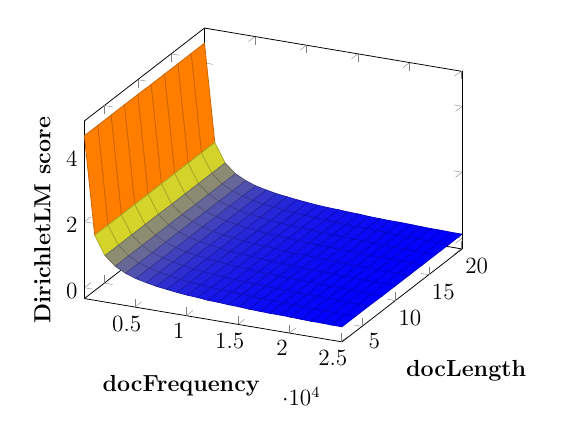
\begin{tikzpicture}[thick,scale=0.7, every node/.style={transform shape}] \begin{axis}[
 %title={},
 %y dir=reverse, 
 %x dir=reverse, 
 ylabel={docLength},
 xlabel={docFrequency},
 zlabel={DirichletLM score},
 every axis/.append style={font=\large\bfseries},
 max space between ticks=25pt
% yticklabels={0k,100k}
 ] 

		\addplot3[surf] coordinates { 
%patch,patch type=biquadratic, shader=faceted,patch refines=3
(100.00,20.00,4.60)(100.00,18.00,4.60)(100.00,16.00,4.60)(100.00,14.00,4.60)(100.00,12.00,4.60)(100.00,10.00,4.61)(100.00,8.00,4.61)(100.00,6.00,4.61)(100.00,4.00,4.61)(100.00,2.00,4.61)

(1100.00,20.00,1.64)(1100.00,18.00,1.64)(1100.00,16.00,1.64)(1100.00,14.00,1.64)(1100.00,12.00,1.64)(1100.00,10.00,1.64)(1100.00,8.00,1.64)(1100.00,6.00,1.64)(1100.00,4.00,1.64)(1100.00,2.00,1.65)

(2100.00,20.00,1.07)(2100.00,18.00,1.07)(2100.00,16.00,1.07)(2100.00,14.00,1.07)(2100.00,12.00,1.07)(2100.00,10.00,1.08)(2100.00,8.00,1.08)(2100.00,6.00,1.08)(2100.00,4.00,1.08)(2100.00,2.00,1.08)

(3100.00,20.00,0.80)(3100.00,18.00,0.80)(3100.00,16.00,0.80)(3100.00,14.00,0.80)(3100.00,12.00,0.81)(3100.00,10.00,0.81)(3100.00,8.00,0.81)(3100.00,6.00,0.81)(3100.00,4.00,0.81)(3100.00,2.00,0.81)

(4100.00,20.00,0.64)(4100.00,18.00,0.64)(4100.00,16.00,0.64)(4100.00,14.00,0.64)(4100.00,12.00,0.65)(4100.00,10.00,0.65)(4100.00,8.00,0.65)(4100.00,6.00,0.65)(4100.00,4.00,0.65)(4100.00,2.00,0.65)

(5100.00,20.00,0.53)(5100.00,18.00,0.54)(5100.00,16.00,0.54)(5100.00,14.00,0.54)(5100.00,12.00,0.54)(5100.00,10.00,0.54)(5100.00,8.00,0.54)(5100.00,6.00,0.54)(5100.00,4.00,0.54)(5100.00,2.00,0.54)

(6100.00,20.00,0.46)(6100.00,18.00,0.46)(6100.00,16.00,0.46)(6100.00,14.00,0.46)(6100.00,12.00,0.46)(6100.00,10.00,0.46)(6100.00,8.00,0.46)(6100.00,6.00,0.47)(6100.00,4.00,0.47)(6100.00,2.00,0.47)

(7100.00,20.00,0.40)(7100.00,18.00,0.40)(7100.00,16.00,0.40)(7100.00,14.00,0.40)(7100.00,12.00,0.40)(7100.00,10.00,0.41)(7100.00,8.00,0.41)(7100.00,6.00,0.41)(7100.00,4.00,0.41)(7100.00,2.00,0.41)

(8100.00,20.00,0.36)(8100.00,18.00,0.36)(8100.00,16.00,0.36)(8100.00,14.00,0.36)(8100.00,12.00,0.36)(8100.00,10.00,0.36)(8100.00,8.00,0.36)(8100.00,6.00,0.36)(8100.00,4.00,0.36)(8100.00,2.00,0.37)

(9100.00,20.00,0.32)(9100.00,18.00,0.32)(9100.00,16.00,0.32)(9100.00,14.00,0.32)(9100.00,12.00,0.32)(9100.00,10.00,0.32)(9100.00,8.00,0.33)(9100.00,6.00,0.33)(9100.00,4.00,0.33)(9100.00,2.00,0.33)

(10100.00,20.00,0.29)(10100.00,18.00,0.29)(10100.00,16.00,0.29)(10100.00,14.00,0.29)(10100.00,12.00,0.29)(10100.00,10.00,0.30)(10100.00,8.00,0.30)(10100.00,6.00,0.30)(10100.00,4.00,0.30)(10100.00,2.00,0.30)

(11100.00,20.00,0.26)(11100.00,18.00,0.27)(11100.00,16.00,0.27)(11100.00,14.00,0.27)(11100.00,12.00,0.27)(11100.00,10.00,0.27)(11100.00,8.00,0.27)(11100.00,6.00,0.27)(11100.00,4.00,0.27)(11100.00,2.00,0.28)

(12100.00,20.00,0.24)(12100.00,18.00,0.25)(12100.00,16.00,0.25)(12100.00,14.00,0.25)(12100.00,12.00,0.25)(12100.00,10.00,0.25)(12100.00,8.00,0.25)(12100.00,6.00,0.25)(12100.00,4.00,0.25)(12100.00,2.00,0.25)

(13100.00,20.00,0.23)(13100.00,18.00,0.23)(13100.00,16.00,0.23)(13100.00,14.00,0.23)(13100.00,12.00,0.23)(13100.00,10.00,0.23)(13100.00,8.00,0.23)(13100.00,6.00,0.23)(13100.00,4.00,0.24)(13100.00,2.00,0.24)

(14100.00,20.00,0.21)(14100.00,18.00,0.21)(14100.00,16.00,0.21)(14100.00,14.00,0.21)(14100.00,12.00,0.21)(14100.00,10.00,0.22)(14100.00,8.00,0.22)(14100.00,6.00,0.22)(14100.00,4.00,0.22)(14100.00,2.00,0.22)

(15100.00,20.00,0.20)(15100.00,18.00,0.20)(15100.00,16.00,0.20)(15100.00,14.00,0.20)(15100.00,12.00,0.20)(15100.00,10.00,0.20)(15100.00,8.00,0.20)(15100.00,6.00,0.20)(15100.00,4.00,0.21)(15100.00,2.00,0.21)

(16100.00,20.00,0.18)(16100.00,18.00,0.19)(16100.00,16.00,0.19)(16100.00,14.00,0.19)(16100.00,12.00,0.19)(16100.00,10.00,0.19)(16100.00,8.00,0.19)(16100.00,6.00,0.19)(16100.00,4.00,0.19)(16100.00,2.00,0.19)

(17100.00,20.00,0.17)(17100.00,18.00,0.18)(17100.00,16.00,0.18)(17100.00,14.00,0.18)(17100.00,12.00,0.18)(17100.00,10.00,0.18)(17100.00,8.00,0.18)(17100.00,6.00,0.18)(17100.00,4.00,0.18)(17100.00,2.00,0.18)

(18100.00,20.00,0.16)(18100.00,18.00,0.17)(18100.00,16.00,0.17)(18100.00,14.00,0.17)(18100.00,12.00,0.17)(18100.00,10.00,0.17)(18100.00,8.00,0.17)(18100.00,6.00,0.17)(18100.00,4.00,0.17)(18100.00,2.00,0.17)

(19100.00,20.00,0.16)(19100.00,18.00,0.16)(19100.00,16.00,0.16)(19100.00,14.00,0.16)(19100.00,12.00,0.16)(19100.00,10.00,0.16)(19100.00,8.00,0.16)(19100.00,6.00,0.16)(19100.00,4.00,0.16)(19100.00,2.00,0.17)

(20100.00,20.00,0.15)(20100.00,18.00,0.15)(20100.00,16.00,0.15)(20100.00,14.00,0.15)(20100.00,12.00,0.15)(20100.00,10.00,0.15)(20100.00,8.00,0.15)(20100.00,6.00,0.16)(20100.00,4.00,0.16)(20100.00,2.00,0.16)

(21100.00,20.00,0.14)(21100.00,18.00,0.14)(21100.00,16.00,0.14)(21100.00,14.00,0.14)(21100.00,12.00,0.15)(21100.00,10.00,0.15)(21100.00,8.00,0.15)(21100.00,6.00,0.15)(21100.00,4.00,0.15)(21100.00,2.00,0.15)

(22100.00,20.00,0.13)(22100.00,18.00,0.14)(22100.00,16.00,0.14)(22100.00,14.00,0.14)(22100.00,12.00,0.14)(22100.00,10.00,0.14)(22100.00,8.00,0.14)(22100.00,6.00,0.14)(22100.00,4.00,0.14)(22100.00,2.00,0.14)

(23100.00,20.00,0.13)(23100.00,18.00,0.13)(23100.00,16.00,0.13)(23100.00,14.00,0.13)(23100.00,12.00,0.13)(23100.00,10.00,0.13)(23100.00,8.00,0.13)(23100.00,6.00,0.14)(23100.00,4.00,0.14)(23100.00,2.00,0.14)

(24100.00,20.00,0.12)(24100.00,18.00,0.12)(24100.00,16.00,0.12)(24100.00,14.00,0.13)(24100.00,12.00,0.13)(24100.00,10.00,0.13)(24100.00,8.00,0.13)(24100.00,6.00,0.13)(24100.00,4.00,0.13)(24100.00,2.00,0.13)

(25100.00,20.00,0.12)(25100.00,18.00,0.12)(25100.00,16.00,0.12)(25100.00,14.00,0.12)(25100.00,12.00,0.12)(25100.00,10.00,0.12)(25100.00,8.00,0.12)(25100.00,6.00,0.13)(25100.00,4.00,0.13)(25100.00,2.00,0.13)

%(26100.00,20.00,0.11)(26100.00,18.00,0.11)(26100.00,16.00,0.11)(26100.00,14.00,0.12)(26100.00,12.00,0.12)(26100.00,10.00,0.12)(26100.00,8.00,0.12)(26100.00,6.00,0.12)(26100.00,4.00,0.12)(26100.00,2.00,0.12)
%
%(27100.00,20.00,0.11)(27100.00,18.00,0.11)(27100.00,16.00,0.11)(27100.00,14.00,0.11)(27100.00,12.00,0.11)(27100.00,10.00,0.11)(27100.00,8.00,0.12)(27100.00,6.00,0.12)(27100.00,4.00,0.12)(27100.00,2.00,0.12)
%
%(28100.00,20.00,0.10)(28100.00,18.00,0.11)(28100.00,16.00,0.11)(28100.00,14.00,0.11)(28100.00,12.00,0.11)(28100.00,10.00,0.11)(28100.00,8.00,0.11)(28100.00,6.00,0.11)(28100.00,4.00,0.11)(28100.00,2.00,0.11)
%
%(29100.00,20.00,0.10)(29100.00,18.00,0.10)(29100.00,16.00,0.10)(29100.00,14.00,0.10)(29100.00,12.00,0.10)(29100.00,10.00,0.11)(29100.00,8.00,0.11)(29100.00,6.00,0.11)(29100.00,4.00,0.11)(29100.00,2.00,0.11)
%
%(30100.00,20.00,0.10)(30100.00,18.00,0.10)(30100.00,16.00,0.10)(30100.00,14.00,0.10)(30100.00,12.00,0.10)(30100.00,10.00,0.10)(30100.00,8.00,0.10)(30100.00,6.00,0.10)(30100.00,4.00,0.11)(30100.00,2.00,0.11)
%
%(31100.00,20.00,0.09)(31100.00,18.00,0.09)(31100.00,16.00,0.10)(31100.00,14.00,0.10)(31100.00,12.00,0.10)(31100.00,10.00,0.10)(31100.00,8.00,0.10)(31100.00,6.00,0.10)(31100.00,4.00,0.10)(31100.00,2.00,0.10)
%
%(32100.00,20.00,0.09)(32100.00,18.00,0.09)(32100.00,16.00,0.09)(32100.00,14.00,0.09)(32100.00,12.00,0.09)(32100.00,10.00,0.10)(32100.00,8.00,0.10)(32100.00,6.00,0.10)(32100.00,4.00,0.10)(32100.00,2.00,0.10)
%
%(33100.00,20.00,0.09)(33100.00,18.00,0.09)(33100.00,16.00,0.09)(33100.00,14.00,0.09)(33100.00,12.00,0.09)(33100.00,10.00,0.09)(33100.00,8.00,0.09)(33100.00,6.00,0.10)(33100.00,4.00,0.10)(33100.00,2.00,0.10)
%
%(34100.00,20.00,0.08)(34100.00,18.00,0.09)(34100.00,16.00,0.09)(34100.00,14.00,0.09)(34100.00,12.00,0.09)(34100.00,10.00,0.09)(34100.00,8.00,0.09)(34100.00,6.00,0.09)(34100.00,4.00,0.09)(34100.00,2.00,0.09)
%
%(35100.00,20.00,0.08)(35100.00,18.00,0.08)(35100.00,16.00,0.08)(35100.00,14.00,0.09)(35100.00,12.00,0.09)(35100.00,10.00,0.09)(35100.00,8.00,0.09)(35100.00,6.00,0.09)(35100.00,4.00,0.09)(35100.00,2.00,0.09)
%
%(36100.00,20.00,0.08)(36100.00,18.00,0.08)(36100.00,16.00,0.08)(36100.00,14.00,0.08)(36100.00,12.00,0.08)(36100.00,10.00,0.09)(36100.00,8.00,0.09)(36100.00,6.00,0.09)(36100.00,4.00,0.09)(36100.00,2.00,0.09)
%
%(37100.00,20.00,0.08)(37100.00,18.00,0.08)(37100.00,16.00,0.08)(37100.00,14.00,0.08)(37100.00,12.00,0.08)(37100.00,10.00,0.08)(37100.00,8.00,0.08)(37100.00,6.00,0.08)(37100.00,4.00,0.09)(37100.00,2.00,0.09)
%
%(38100.00,20.00,0.07)(38100.00,18.00,0.08)(38100.00,16.00,0.08)(38100.00,14.00,0.08)(38100.00,12.00,0.08)(38100.00,10.00,0.08)(38100.00,8.00,0.08)(38100.00,6.00,0.08)(38100.00,4.00,0.08)(38100.00,2.00,0.08)
%
%(39100.00,20.00,0.07)(39100.00,18.00,0.07)(39100.00,16.00,0.07)(39100.00,14.00,0.08)(39100.00,12.00,0.08)(39100.00,10.00,0.08)(39100.00,8.00,0.08)(39100.00,6.00,0.08)(39100.00,4.00,0.08)(39100.00,2.00,0.08)
%
%(40100.00,20.00,0.07)(40100.00,18.00,0.07)(40100.00,16.00,0.07)(40100.00,14.00,0.07)(40100.00,12.00,0.08)(40100.00,10.00,0.08)(40100.00,8.00,0.08)(40100.00,6.00,0.08)(40100.00,4.00,0.08)(40100.00,2.00,0.08)
%
%(41100.00,20.00,0.07)(41100.00,18.00,0.07)(41100.00,16.00,0.07)(41100.00,14.00,0.07)(41100.00,12.00,0.07)(41100.00,10.00,0.07)(41100.00,8.00,0.08)(41100.00,6.00,0.08)(41100.00,4.00,0.08)(41100.00,2.00,0.08)
%
%(42100.00,20.00,0.07)(42100.00,18.00,0.07)(42100.00,16.00,0.07)(42100.00,14.00,0.07)(42100.00,12.00,0.07)(42100.00,10.00,0.07)(42100.00,8.00,0.07)(42100.00,6.00,0.07)(42100.00,4.00,0.08)(42100.00,2.00,0.08)
%
%(43100.00,20.00,0.06)(43100.00,18.00,0.07)(43100.00,16.00,0.07)(43100.00,14.00,0.07)(43100.00,12.00,0.07)(43100.00,10.00,0.07)(43100.00,8.00,0.07)(43100.00,6.00,0.07)(43100.00,4.00,0.07)(43100.00,2.00,0.08)
%
%(44100.00,20.00,0.06)(44100.00,18.00,0.06)(44100.00,16.00,0.07)(44100.00,14.00,0.07)(44100.00,12.00,0.07)(44100.00,10.00,0.07)(44100.00,8.00,0.07)(44100.00,6.00,0.07)(44100.00,4.00,0.07)(44100.00,2.00,0.07)
%
%(45100.00,20.00,0.06)(45100.00,18.00,0.06)(45100.00,16.00,0.06)(45100.00,14.00,0.07)(45100.00,12.00,0.07)(45100.00,10.00,0.07)(45100.00,8.00,0.07)(45100.00,6.00,0.07)(45100.00,4.00,0.07)(45100.00,2.00,0.07)
%
%(46100.00,20.00,0.06)(46100.00,18.00,0.06)(46100.00,16.00,0.06)(46100.00,14.00,0.06)(46100.00,12.00,0.06)(46100.00,10.00,0.07)(46100.00,8.00,0.07)(46100.00,6.00,0.07)(46100.00,4.00,0.07)(46100.00,2.00,0.07)
%
%(47100.00,20.00,0.06)(47100.00,18.00,0.06)(47100.00,16.00,0.06)(47100.00,14.00,0.06)(47100.00,12.00,0.06)(47100.00,10.00,0.06)(47100.00,8.00,0.07)(47100.00,6.00,0.07)(47100.00,4.00,0.07)(47100.00,2.00,0.07)
%
%(48100.00,20.00,0.06)(48100.00,18.00,0.06)(48100.00,16.00,0.06)(48100.00,14.00,0.06)(48100.00,12.00,0.06)(48100.00,10.00,0.06)(48100.00,8.00,0.06)(48100.00,6.00,0.07)(48100.00,4.00,0.07)(48100.00,2.00,0.07)
%
%(49100.00,20.00,0.06)(49100.00,18.00,0.06)(49100.00,16.00,0.06)(49100.00,14.00,0.06)(49100.00,12.00,0.06)(49100.00,10.00,0.06)(49100.00,8.00,0.06)(49100.00,6.00,0.06)(49100.00,4.00,0.06)(49100.00,2.00,0.07)


}; \end{axis} \end{tikzpicture}

          \label{dlmproof}          
        \end{subfigure}

        \caption{DLM evaluation figures}
\end{figure}

Figures \ref{dlmproofc2} and \ref{dlmproofcc} show DLM scores in terms of the $\mu$ parameter, w.r.t. document frequency and document length respectively. Figure \ref{dlmproof} on the other hand demonstrates the relation between document frequency and document length.

As we can observe from Equation \ref{dlmequation} the parameter $\mu$ is closely related to the collection statistics of the terms, and the length normalization component of the equation. Moreover the lower the values of $\mu$ the higher the score differences for similar document frequencies as shown in Figure \ref{dlmproofc2}. Similarly, we can observe in Figure \ref{dlmproofcc} how $\mu$ interacts with document length. For low values of $\mu$ we can observe how the scores are reduced at the same time that documents become larger, as expected. Interestingly, this behaviour is dampened with higher values of $\mu$, as score differences are heavily reduced w.r.t. the different document lengths. Since the default value for $\mu$ is 2500, it is no surprise that document length has virtually no effect over the scores for DLM  as seen in Figure \ref{dlmproof}, contrary to other retrieval models. 

\begin{table}[]

	\caption{P@30 scores for DLM for a range of $\mu$ values}
	\centering
	\begin{tabular}{l|c} 	
	\textit{\textbf{$\mu$}} & 
	\textit{\textbf{P@30}} 	
	\tabularnewline
	\hline
	1 & 0.4028 \\
	5 &  0.4164 \\
	20 & 0.4241 \\
	50 &  0.4099 \\
	100 &  0.3933 \\
	500 &  0.3396 \\
	1000 & 0.3227 \\
	2500 & 0.2988 \\
	\hline	
	\end{tabular}
	\label{drmmuvalues}
\end{table}

This could be a desired feature for microblog retrieval, however let us look at the performance achieved for a range of $\mu$ values in Table \ref{drmmuvalues}. As we can observe generally the higher the value of $mu$ the worse the performance obtained, with the exception of $\mu$ within the 1 to 20 range. 

In order to further understand the behaviour of DLM in the case of Microblog retrieval, we repeat the same experiment we performed for HLM in the previous Section. We assume that since DLM was also designed for bigger documents than microblogs, overestimating the statistics of TF and DL can be interesting experiment as it would better resemble its standard behaviour in term of the numerical values produced as scores. 

The resulting evaluation metrics for such runs are presented in Table \ref{drmdtfmuvalues}. The first four lines contain the P@30 values for different combinations where $\mu$ is set to 20. As we can observe overestimating TF by +20 results in a substantial +7.47\% increase of P@30 with respect to the default configuration. On the other hand overestimating DL by +20 results in a 8.02\% decrease of performance in terms of P@30. Finally, combining both TF and DL overestimates results in comparable performance than that obtained by only increasing TF.

\begin{table}[]
	\caption{P@30 scores for DLM as we consider different combinations of dTF and dDL, and $\mu$}
	\centering
	\begin{tabular}{l|c|c|c} 	
	\textit{\textbf{$\mu$}} & 
	\textit{\textbf{dTF}} & 
	\textit{\textbf{dDL}} & 
	\textit{\textbf{P@30}} 	
	\tabularnewline
	\hline
	20 &    &    & 0.4241\\
	20 & 20 &    & 0.4558\\
	20 &    & 20 & 0.3901\\
	20 & 20 & 20 & 0.4547\\
	\hline	
	\hline
	2500 &    &    & 0.2988\\
	2500 & 20 &    & 0.4468\\
	2500 &    & 20 & 0.2892\\
	2500 & 20 & 20 & 0.4466\\
    \hline
	\end{tabular}
	\label{drmdtfmuvalues}
\end{table}

The same behaviour is obtained across all combinations when we set the $\mu = 2500$. To further develop our understanding of the behaviour, and to draw conclusions for such results, we devised Figures \ref{dlmfigureTFDL2500} and \ref{dlmfigureTFDL20}. Figures \ref{dlmfigureTFDL2500} and \ref{dlmfigureTFDL20} present the DLM scores produced with respect to Doc. Length and Term Frequency (TF) when $\mu=2500$ and $\mu=20$ respectively.

Let us analyse the results from Table \ref{drmdtfmuvalues} in connection with Figures \ref{dlmfigureTFDL2500} and \ref{dlmfigureTFDL20}. As we can observe incrementing DL will result in an increased differentiation of DLM scores with respect to TF as more values are closer to the minimum and maximum values. In other words there are less intermediate values (Light coloured areas), which ultimately reflects on heightened sensitivity to differences across the TF spectrum. Furthermore, we can also observe in Table \ref{drmdtfmuvalues} how incrementing DL values, results in worse performance in all cases. Consequently the increased differentiation of DLM scores with respect to the TF parameter, produced by the increment of DL is detrimental and in line with the findings in the previous section.

Additionally, Figure \ref{dlmfigureTFDL2500} shows an almost linear progression of DLM scores with respect to TF. Furthermore, Figure \ref{dlmfigureTFDL20} where $\mu=20$ exhibits a logarithmic behaviour with respect to TF. The latter behaviour is more desirable because there should be a saturation point when incrementing TF at which there is very little value added to the score of the document, or could be even counter productive.

The better behaviour with respect to TF is rewarded with increased performance whether the value of $\mu$ is 20 or 2500. In fact the offsetting of TF seems to overrule the effects of $\mu$ as similar results are obtained in both $\mu=20$ and $\mu=2500$ conditions. The effects of offsetting TF are most visually evident when looking at Figure \ref{dlmfigureTFDL20} as differences amongst the different scores become very small. 


\begin{figure}
      	\begin{subfigure}[b]{0.5\textwidth}
          \centering
          \caption{Doc. length (DL) and Term Frequency (TF) when $\mu = 2500$}
          
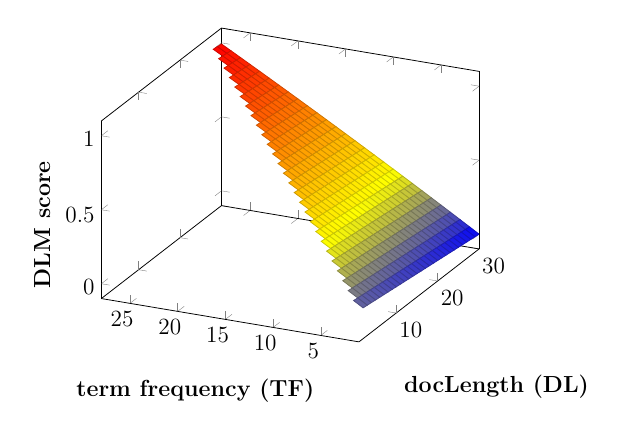
\begin{tikzpicture}[thick,scale=0.7, every node/.style={transform shape}]\begin{axis}[
 %title={},
 %y dir=reverse, 
 x dir=reverse, 
 xlabel={term frequency (TF)},
 ylabel={docLength (DL)},
 zlabel={DLM score},
 every axis/.append style={font=\large\bfseries},
 max space between ticks=25pt
% yticklabels={0k,100k}
 ] 

\addplot3[surf,unbounded coords=jump] coordinates { 
%patch,patch type=biquadratic, shader=faceted,patch refines=3
(1,1,0.111973219732543)	(2,1,nan)	(3,1,nan)	(4,1,nan)	(5,1,nan)	(6,1,nan)	(7,1,nan)	(8,1,nan)	(9,1,nan)	(10,1,nan)	(11,1,nan)	(12,1,nan)	(13,1,nan)	(14,1,nan)	(15,1,nan)	(16,1,nan)	(17,1,nan)	(18,1,nan)	(19,1,nan)	(20,1,nan)	(21,1,nan)	(22,1,nan)	(23,1,nan)	(24,1,nan)	(25,1,nan)	(26,1,nan)	(27,1,nan)	(28,1,nan)

(1,2,0.108090507727749)	(2,2,0.146709262188192)	(3,2,nan)	(4,2,nan)	(5,2,nan)	(6,2,nan)	(7,2,nan)	(8,2,nan)	(9,2,nan)	(10,2,nan)	(11,2,nan)	(12,2,nan)	(13,2,nan)	(14,2,nan)	(15,2,nan)	(16,2,nan)	(17,2,nan)	(18,2,nan)	(19,2,nan)	(20,2,nan)	(21,2,nan)	(22,2,nan)	(23,2,nan)	(24,2,nan)	(25,2,nan)	(26,2,nan)	(27,2,nan)	(28,2,nan)

(1,3,0.104209347256264)	(2,3,0.142828101716707)	(3,3,0.181293910214315)	(4,3,nan)	(5,3,nan)	(6,3,nan)	(7,3,nan)	(8,3,nan)	(9,3,nan)	(10,3,nan)	(11,3,nan)	(12,3,nan)	(13,3,nan)	(14,3,nan)	(15,3,nan)	(16,3,nan)	(17,3,nan)	(18,3,nan)	(19,3,nan)	(20,3,nan)	(21,3,nan)	(22,3,nan)	(23,3,nan)	(24,3,nan)	(25,3,nan)	(26,3,nan)	(27,3,nan)	(28,3,nan)

(1,4,0.100329737078599)	(2,4,0.138948491539042)	(3,4,0.17741430003665)	(4,4,0.2157283692504)	(5,4,nan)	(6,4,nan)	(7,4,nan)	(8,4,nan)	(9,4,nan)	(10,4,nan)	(11,4,nan)	(12,4,nan)	(13,4,nan)	(14,4,nan)	(15,4,nan)	(16,4,nan)	(17,4,nan)	(18,4,nan)	(19,4,nan)	(20,4,nan)	(21,4,nan)	(22,4,nan)	(23,4,nan)	(24,4,nan)	(25,4,nan)	(26,4,nan)	(27,4,nan)	(28,4,nan)

(1,5,0.0964516759567444)	(2,5,0.135070430417187)	(3,5,0.173536238914795)	(4,5,0.211850308128545)	(5,5,0.250013830513225)	(6,5,nan)	(7,5,nan)	(8,5,nan)	(9,5,nan)	(10,5,nan)	(11,5,nan)	(12,5,nan)	(13,5,nan)	(14,5,nan)	(15,5,nan)	(16,5,nan)	(17,5,nan)	(18,5,nan)	(19,5,nan)	(20,5,nan)	(21,5,nan)	(22,5,nan)	(23,5,nan)	(24,5,nan)	(25,5,nan)	(26,5,nan)	(27,5,nan)	(28,5,nan)

(1,6,0.0925751626541784)	(2,6,0.131193917114621)	(3,6,0.169659725612229)	(4,6,0.207973794825979)	(5,6,0.246137317210659)	(6,6,0.284151471219561)	(7,6,nan)	(8,6,nan)	(9,6,nan)	(10,6,nan)	(11,6,nan)	(12,6,nan)	(13,6,nan)	(14,6,nan)	(15,6,nan)	(16,6,nan)	(17,6,nan)	(18,6,nan)	(19,6,nan)	(20,6,nan)	(21,6,nan)	(22,6,nan)	(23,6,nan)	(24,6,nan)	(25,6,nan)	(26,6,nan)	(27,6,nan)	(28,6,nan)

(1,7,0.0887001959358549)	(2,7,0.127318950396297)	(3,7,0.165784758893906)	(4,7,0.204098828107656)	(5,7,0.242262350492336)	(6,7,0.280276504501237)	(7,7,0.318142454804501)	(8,7,nan)	(9,7,nan)	(10,7,nan)	(11,7,nan)	(12,7,nan)	(13,7,nan)	(14,7,nan)	(15,7,nan)	(16,7,nan)	(17,7,nan)	(18,7,nan)	(19,7,nan)	(20,7,nan)	(21,7,nan)	(22,7,nan)	(23,7,nan)	(24,7,nan)	(25,7,nan)	(26,7,nan)	(27,7,nan)	(28,7,nan)

(1,8,0.0848267745682088)	(2,8,0.123445529028651)	(3,8,0.16191133752626)	(4,8,0.200225406740009)	(5,8,0.23838892912469)	(6,8,0.276403083133591)	(7,8,0.314269033436855)	(8,8,0.35198793113558)	(9,8,nan)	(10,8,nan)	(11,8,nan)	(12,8,nan)	(13,8,nan)	(14,8,nan)	(15,8,nan)	(16,8,nan)	(17,8,nan)	(18,8,nan)	(19,8,nan)	(20,8,nan)	(21,8,nan)	(22,8,nan)	(23,8,nan)	(24,8,nan)	(25,8,nan)	(26,8,nan)	(27,8,nan)	(28,8,nan)

(1,9,0.0809548973191464)	(2,9,0.119573651779589)	(3,9,0.158039460277197)	(4,9,0.196353529490947)	(5,9,0.234517051875627)	(6,9,0.272531205884529)	(7,9,0.310397156187792)	(8,9,0.348116053886518)	(9,9,0.385689036722731)	(10,9,nan)	(11,9,nan)	(12,9,nan)	(13,9,nan)	(14,9,nan)	(15,9,nan)	(16,9,nan)	(17,9,nan)	(18,9,nan)	(19,9,nan)	(20,9,nan)	(21,9,nan)	(22,9,nan)	(23,9,nan)	(24,9,nan)	(25,9,nan)	(26,9,nan)	(27,9,nan)	(28,9,nan)

(1,10,0.0770845629580511)	(2,10,0.115703317418494)	(3,10,0.154169125916102)	(4,10,0.192483195129852)	(5,10,0.230646717514532)	(6,10,0.268660871523434)	(7,10,0.306526821826697)	(8,10,0.344245719525422)	(9,10,0.381818702361636)	(10,10,0.41924689492421)	(11,10,nan)	(12,10,nan)	(13,10,nan)	(14,10,nan)	(15,10,nan)	(16,10,nan)	(17,10,nan)	(18,10,nan)	(19,10,nan)	(20,10,nan)	(21,10,nan)	(22,10,nan)	(23,10,nan)	(24,10,nan)	(25,10,nan)	(26,10,nan)	(27,10,nan)	(28,10,nan)

(1,11,0.0732157702557744)	(2,11,0.111834524716217)	(3,11,0.150300333213825)	(4,11,0.188614402427575)	(5,11,0.226777924812255)	(6,11,0.264792078821157)	(7,11,0.30265802912442)	(8,11,0.340376926823146)	(9,11,0.377949909659359)	(10,11,0.415378102221933)	(11,11,0.452662616148559)	(12,11,nan)	(13,11,nan)	(14,11,nan)	(15,11,nan)	(16,11,nan)	(17,11,nan)	(18,11,nan)	(19,11,nan)	(20,11,nan)	(21,11,nan)	(22,11,nan)	(23,11,nan)	(24,11,nan)	(25,11,nan)	(26,11,nan)	(27,11,nan)	(28,11,nan)

(1,12,0.0693485179846348)	(2,12,0.107967272445077)	(3,12,0.146433080942686)	(4,12,0.184747150156436)	(5,12,0.222910672541116)	(6,12,0.260924826550017)	(7,12,0.298790776853281)	(8,12,0.336509674552006)	(9,12,0.374082657388219)	(10,12,0.411510849950794)	(11,12,0.448795363877419)	(12,12,0.48593729805271)	(13,12,nan)	(14,12,nan)	(15,12,nan)	(16,12,nan)	(17,12,nan)	(18,12,nan)	(19,12,nan)	(20,12,nan)	(21,12,nan)	(22,12,nan)	(23,12,nan)	(24,12,nan)	(25,12,nan)	(26,12,nan)	(27,12,nan)	(28,12,nan)

(1,13,0.0654828049184215)	(2,13,0.104101559378864)	(3,13,0.142567367876472)	(4,13,0.180881437090222)	(5,13,0.219044959474903)	(6,13,0.257059113483804)	(7,13,0.294925063787067)	(8,13,0.332643961485793)	(9,13,0.370216944322006)	(10,13,0.40764513688458)	(11,13,0.444929650811206)	(12,13,0.482071584986497)	(13,13,0.519072025736323)	(14,13,nan)	(15,13,nan)	(16,13,nan)	(17,13,nan)	(18,13,nan)	(19,13,nan)	(20,13,nan)	(21,13,nan)	(22,13,nan)	(23,13,nan)	(24,13,nan)	(25,13,nan)	(26,13,nan)	(27,13,nan)	(28,13,nan)

(1,14,0.0616186298323818)	(2,14,0.100237384292824)	(3,14,0.138703192790433)	(4,14,0.177017262004182)	(5,14,0.215180784388863)	(6,14,0.253194938397764)	(7,14,0.291060888701028)	(8,14,0.328779786399753)	(9,14,0.366352769235966)	(10,14,0.403780961798541)	(11,14,0.441065475725166)	(12,14,0.478207409900457)	(13,14,0.515207850650284)	(14,14,0.552067871932422)	(15,14,nan)	(16,14,nan)	(17,14,nan)	(18,14,nan)	(19,14,nan)	(20,14,nan)	(21,14,nan)	(22,14,nan)	(23,14,nan)	(24,14,nan)	(25,14,nan)	(26,14,nan)	(27,14,nan)	(28,14,nan)

(1,15,0.0577559915032278)	(2,15,0.0963747459636703)	(3,15,0.134840554461279)	(4,15,0.173154623675029)	(5,15,0.211318146059709)	(6,15,0.24933230006861)	(7,15,0.287198250371874)	(8,15,0.324917148070599)	(9,15,0.362490130906812)	(10,15,0.399918323469387)	(11,15,0.437202837396012)	(12,15,0.474344771571303)	(13,15,0.51134521232113)	(14,15,0.548205233603268)	(15,15,0.584925897194439)	(16,15,nan)	(17,15,nan)	(18,15,nan)	(19,15,nan)	(20,15,nan)	(21,15,nan)	(22,15,nan)	(23,15,nan)	(24,15,nan)	(25,15,nan)	(26,15,nan)	(27,15,nan)	(28,15,nan)

(1,16,0.053894888709128)	(2,16,0.0925136431695705)	(3,16,0.130979451667179)	(4,16,0.169293520880929)	(5,16,0.207457043265609)	(6,16,0.24547119727451)	(7,16,0.283337147577774)	(8,16,0.321056045276499)	(9,16,0.358629028112712)	(10,16,0.396057220675287)	(11,16,0.433341734601912)	(12,16,0.470483668777203)	(13,16,0.50748410952703)	(14,16,0.544344130809168)	(15,16,0.581064794400339)	(16,16,0.61764715007973)	(17,16,nan)	(18,16,nan)	(19,16,nan)	(20,16,nan)	(21,16,nan)	(22,16,nan)	(23,16,nan)	(24,16,nan)	(25,16,nan)	(26,16,nan)	(27,16,nan)	(28,16,nan)

(1,17,0.0500353202297106)	(2,17,0.0886540746901531)	(3,17,0.127119883187761)	(4,17,0.165433952401511)	(5,17,0.203597474786192)	(6,17,0.241611628795093)	(7,17,0.279477579098356)	(8,17,0.317196476797082)	(9,17,0.354769459633295)	(10,17,0.392197652195869)	(11,17,0.429482166122495)	(12,17,0.466624100297786)	(13,17,0.503624541047612)	(14,17,0.540484562329751)	(15,17,0.577205225920921)	(16,17,0.613787581600312)	(17,17,0.650232667329652)	(18,17,nan)	(19,17,nan)	(20,17,nan)	(21,17,nan)	(22,17,nan)	(23,17,nan)	(24,17,nan)	(25,17,nan)	(26,17,nan)	(27,17,nan)	(28,17,nan)

(1,18,0.0461772848460546)	(2,18,0.0847960393064971)	(3,18,0.123261847804105)	(4,18,0.161575917017855)	(5,18,0.199739439402536)	(6,18,0.237753593411437)	(7,18,0.2756195437147)	(8,18,0.313338441413426)	(9,18,0.350911424249639)	(10,18,0.388339616812213)	(11,18,0.425624130738839)	(12,18,0.46276606491413)	(13,18,0.499766505663956)	(14,18,0.536626526946095)	(15,18,0.573347190537265)	(16,18,0.609929546216656)	(17,18,0.646374631945996)	(18,18,0.682683474046268)	(19,18,nan)	(20,18,nan)	(21,18,nan)	(22,18,nan)	(23,18,nan)	(24,18,nan)	(25,18,nan)	(26,18,nan)	(27,18,nan)	(28,18,nan)

(1,19,0.0423207813406933)	(2,19,0.0809395358011359)	(3,19,0.119405344298744)	(4,19,0.157719413512494)	(5,19,0.195882935897174)	(6,19,0.233897089906076)	(7,19,0.271763040209339)	(8,19,0.309481937908065)	(9,19,0.347054920744278)	(10,19,0.384483113306852)	(11,19,0.421767627233478)	(12,19,0.458909561408768)	(13,19,0.495910002158595)	(14,19,0.532770023440733)	(15,19,0.569490687031904)	(16,19,0.606073042711295)	(17,19,0.642518128440635)	(18,19,0.678826970540907)	(19,19,0.715000583865767)	(20,19,nan)	(21,19,nan)	(22,19,nan)	(23,19,nan)	(24,19,nan)	(25,19,nan)	(26,19,nan)	(27,19,nan)	(28,19,nan)

(1,20,0.0384658084976089)	(2,20,0.0770845629580515)	(3,20,0.11555037145566)	(4,20,0.15386444066941)	(5,20,0.19202796305409)	(6,20,0.230042117062991)	(7,20,0.267908067366255)	(8,20,0.30562696506498)	(9,20,0.343199947901193)	(10,20,0.380628140463768)	(11,20,0.417912654390393)	(12,20,0.455054588565684)	(13,20,0.492055029315511)	(14,20,0.528915050597649)	(15,20,0.56563571418882)	(16,20,0.602218069868211)	(17,20,0.638663155597551)	(18,20,0.674971997697823)	(19,20,0.711145611022683)	(20,20,0.747184999128663)	(21,20,nan)	(22,20,nan)	(23,20,nan)	(24,20,nan)	(25,20,nan)	(26,20,nan)	(27,20,nan)	(28,20,nan)

(1,21,0.0346123651022313)	(2,21,0.0732311195626738)	(3,21,0.111696928060282)	(4,21,0.150010997274032)	(5,21,0.188174519658712)	(6,21,0.226188673667614)	(7,21,0.264054623970877)	(8,21,0.301773521669603)	(9,21,0.339346504505816)	(10,21,0.37677469706839)	(11,21,0.414059210995016)	(12,21,0.451201145170306)	(13,21,0.488201585920133)	(14,21,0.525061607202271)	(15,21,0.561782270793442)	(16,21,0.598364626472833)	(17,21,0.634809712202173)	(18,21,0.671118554302445)	(19,21,0.707292167627305)	(20,21,0.743331555733285)	(21,21,0.779237711046848)	(22,21,nan)	(23,21,nan)	(24,21,nan)	(25,21,nan)	(26,21,nan)	(27,21,nan)	(28,21,nan)

(1,22,0.0307604499414344)	(2,22,0.0693792044018769)	(3,22,0.107845012899485)	(4,22,0.146159082113235)	(5,22,0.184322604497915)	(6,22,0.222336758506817)	(7,22,0.26020270881008)	(8,22,0.297921606508806)	(9,22,0.335494589345019)	(10,22,0.372922781907593)	(11,22,0.410207295834219)	(12,22,0.447349230009509)	(13,22,0.484349670759336)	(14,22,0.521209692041474)	(15,22,0.557930355632645)	(16,22,0.594512711312036)	(17,22,0.630957797041376)	(18,22,0.667266639141648)	(19,22,0.703440252466508)	(20,22,0.739479640572488)	(21,22,0.775385795886051)	(22,22,0.811159699867572)	(23,22,nan)	(24,22,nan)	(25,22,nan)	(26,22,nan)	(27,22,nan)	(28,22,nan)

(1,23,0.0269100618035358)	(2,23,0.0655288162639784)	(3,23,0.103994624761587)	(4,23,0.142308693975337)	(5,23,0.180472216360017)	(6,23,0.218486370368918)	(7,23,0.256352320672182)	(8,23,0.294071218370907)	(9,23,0.33164420120712)	(10,23,0.369072393769695)	(11,23,0.40635690769632)	(12,23,0.443498841871611)	(13,23,0.480499282621438)	(14,23,0.517359303903576)	(15,23,0.554079967494747)	(16,23,0.590662323174138)	(17,23,0.627107408903478)	(18,23,0.66341625100375)	(19,23,0.69958986432861)	(20,23,0.73562925243459)	(21,23,0.771535407748152)	(22,23,0.807309311729674)	(23,23,0.842951935034412)	(24,23,nan)	(25,23,nan)	(26,23,nan)	(27,23,nan)	(28,23,nan)

(1,24,0.0230611994782949)	(2,24,0.0616799539387374)	(3,24,0.100145762436346)	(4,24,0.138459831650096)	(5,24,0.176623354034776)	(6,24,0.214637508043677)	(7,24,0.252503458346941)	(8,24,0.290222356045666)	(9,24,0.327795338881879)	(10,24,0.365223531444454)	(11,24,0.402508045371079)	(12,24,0.43964997954637)	(13,24,0.476650420296197)	(14,24,0.513510441578335)	(15,24,0.550231105169506)	(16,24,0.586813460848896)	(17,24,0.623258546578237)	(18,24,0.659567388678509)	(19,24,0.695741002003369)	(20,24,0.731780390109349)	(21,24,0.767686545422911)	(22,24,0.803460449404433)	(23,24,0.839103072709171)	(24,24,0.874615375345294)	(25,24,nan)	(26,24,nan)	(27,24,nan)	(28,24,nan)

(1,25,0.0192138617569053)	(2,25,0.0578326162173479)	(3,25,0.0962984247149561)	(4,25,0.134612493928706)	(5,25,0.172776016313386)	(6,25,0.210790170322288)	(7,25,0.248656120625551)	(8,25,0.286375018324276)	(9,25,0.32394800116049)	(10,25,0.361376193723064)	(11,25,0.39866070764969)	(12,25,0.43580264182498)	(13,25,0.472803082574807)	(14,25,0.509663103856945)	(15,25,0.546383767448116)	(16,25,0.582966123127507)	(17,25,0.619411208856847)	(18,25,0.655720050957119)	(19,25,0.691893664281979)	(20,25,0.727933052387959)	(21,25,0.763839207701522)	(22,25,0.799613111683043)	(23,25,0.835255734987781)	(24,25,0.870768037623905)	(25,25,0.906150969107645)	(26,25,nan)	(27,25,nan)	(28,25,nan)

(1,26,0.0153680474320015)	(2,26,0.053986801892444)	(3,26,0.0924526103900523)	(4,26,0.130766679603802)	(5,26,0.168930201988483)	(6,26,0.206944355997384)	(7,26,0.244810306300647)	(8,26,0.282529203999373)	(9,26,0.320102186835586)	(10,26,0.35753037939816)	(11,26,0.394814893324786)	(12,26,0.431956827500076)	(13,26,0.468957268249903)	(14,26,0.505817289532042)	(15,26,0.542537953123212)	(16,26,0.579120308802603)	(17,26,0.615565394531943)	(18,26,0.651874236632215)	(19,26,0.688047849957076)	(20,26,0.724087238063055)	(21,26,0.759993393376618)	(22,26,0.795767297358139)	(23,26,0.831409920662877)	(24,26,0.866922223299001)	(25,26,0.902305154782741)	(26,26,0.937559654290723)	(27,26,nan)	(28,26,nan)

(1,27,0.0115237552976474)	(2,27,0.0501425097580899)	(3,27,0.0886083182556982)	(4,27,0.126922387469448)	(5,27,0.165085909854128)	(6,27,0.20310006386303)	(7,27,0.240966014166293)	(8,27,0.278684911865019)	(9,27,0.316257894701232)	(10,27,0.353686087263806)	(11,27,0.390970601190432)	(12,27,0.428112535365722)	(13,27,0.465112976115549)	(14,27,0.501972997397687)	(15,27,0.538693660988858)	(16,27,0.575276016668249)	(17,27,0.611721102397589)	(18,27,0.648029944497861)	(19,27,0.684203557822721)	(20,27,0.720242945928701)	(21,27,0.756149101242264)	(22,27,0.791923005223785)	(23,27,0.827565628528523)	(24,27,0.863077931164647)	(25,27,0.898460862648387)	(26,27,0.933715362156369)	(27,27,0.96884235867519)	(28,27,nan)

(1,28,0.00768098414934081)	(2,28,0.0462997386097834)	(3,28,0.0847655471073916)	(4,28,0.123079616321142)	(5,28,0.161243138705822)	(6,28,0.199257292714723)	(7,28,0.237123243017987)	(8,28,0.274842140716712)	(9,28,0.312415123552925)	(10,28,0.3498433161155)	(11,28,0.387127830042125)	(12,28,0.424269764217416)	(13,28,0.461270204967243)	(14,28,0.498130226249381)	(15,28,0.534850889840552)	(16,28,0.571433245519943)	(17,28,0.607878331249283)	(18,28,0.644187173349555)	(19,28,0.680360786674415)	(20,28,0.716400174780395)	(21,28,0.752306330093957)	(22,28,0.788080234075479)	(23,28,0.823722857380217)	(24,28,0.85923516001634)	(25,28,0.894618091500081)	(26,28,0.929872591008062)	(27,28,0.964999587526883)	(28,28,1)

(1,29,0.00383973278400676)	(2,29,0.0424584872444493)	(3,29,0.0809242957420575)	(4,29,0.119238364955807)	(5,29,0.157401887340488)	(6,29,0.195416041349389)	(7,29,0.233281991652653)	(8,29,0.271000889351378)	(9,29,0.308573872187591)	(10,29,0.346002064750166)	(11,29,0.383286578676791)	(12,29,0.420428512852082)	(13,29,0.457428953601909)	(14,29,0.494288974884047)	(15,29,0.531009638475218)	(16,29,0.567591994154608)	(17,29,0.604037079883948)	(18,29,0.640345921984221)	(19,29,0.676519535309081)	(20,29,0.712558923415061)	(21,29,0.748465078728623)	(22,29,0.784238982710144)	(23,29,0.819881606014882)	(24,29,0.855393908651006)	(25,29,0.890776840134747)	(26,29,0.926031339642728)	(27,29,0.961158336161549)	(28,29,0.996158748634666)

(1,30,0)	(2,30,0.0386187544604425)	(3,30,0.0770845629580511)	(4,30,0.115398632171801)	(5,30,0.153562154556481)	(6,30,0.191576308565382)	(7,30,0.229442258868646)	(8,30,0.267161156567371)	(9,30,0.304734139403584)	(10,30,0.342162331966159)	(11,30,0.379446845892784)	(12,30,0.416588780068075)	(13,30,0.453589220817902)	(14,30,0.49044924210004)	(15,30,0.527169905691211)	(16,30,0.563752261370602)	(17,30,0.600197347099942)	(18,30,0.636506189200214)	(19,30,0.672679802525074)	(20,30,0.708719190631054)	(21,30,0.744625345944617)	(22,30,0.780399249926138)	(23,30,0.816041873230876)	(24,30,0.851554175867)	(25,30,0.88693710735074)	(26,30,0.922191606858721)	(27,30,0.957318603377542)	(28,30,0.992319015850659)

}; \end{axis} \end{tikzpicture}

          \label{dlmfigureTFDL2500}          
        \end{subfigure} 
        ~
 		\begin{subfigure}[b]{0.5\textwidth}
          \centering
          \caption{Doc. length (DL) and Term Frequency (TF) when $\mu = 20$}
          
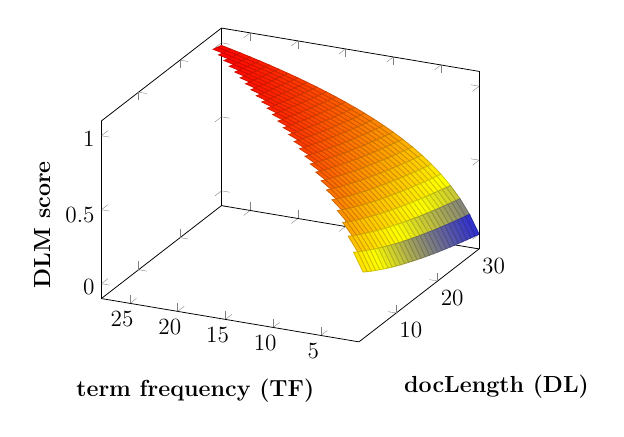
\begin{tikzpicture}[thick,scale=0.7, every node/.style={transform shape}]\begin{axis}[
 %title={},
 %y dir=reverse, 
 x dir=reverse, 
 ylabel={docLength (DL)},
 xlabel={term frequency (TF)},
 zlabel={DLM score},
 every axis/.append style={font=\large\bfseries},
 max space between ticks=25pt
% yticklabels={0k,100k}
 ] 

		\addplot3[surf,unbounded coords=jump] coordinates { 
%patch,patch type=biquadratic, shader=faceted,patch refines=3
(1,1,0.370187737472834)	(2,1,nan)	(3,1,nan)	(4,1,nan)	(5,1,nan)	(6,1,nan)	(7,1,nan)	(8,1,nan)	(9,1,nan)	(10,1,nan)	(11,1,nan)	(12,1,nan)	(13,1,nan)	(14,1,nan)	(15,1,nan)	(16,1,nan)	(17,1,nan)	(18,1,nan)	(19,1,nan)	(20,1,nan)	(21,1,nan)	(22,1,nan)	(23,1,nan)	(24,1,nan)	(25,1,nan)	(26,1,nan)	(27,1,nan)	(28,1,nan)

(1,2,0.35033629301713)	(2,2,0.473098605201195)	(3,2,nan)	(4,2,nan)	(5,2,nan)	(6,2,nan)	(7,2,nan)	(8,2,nan)	(9,2,nan)	(10,2,nan)	(11,2,nan)	(12,2,nan)	(13,2,nan)	(14,2,nan)	(15,2,nan)	(16,2,nan)	(17,2,nan)	(18,2,nan)	(19,2,nan)	(20,2,nan)	(21,2,nan)	(22,2,nan)	(23,2,nan)	(24,2,nan)	(25,2,nan)	(26,2,nan)	(27,2,nan)	(28,2,nan)

(1,3,0.331367432332329)	(2,3,0.454129744516394)	(3,3,0.549351591588173)	(4,3,nan)	(5,3,nan)	(6,3,nan)	(7,3,nan)	(8,3,nan)	(9,3,nan)	(10,3,nan)	(11,3,nan)	(12,3,nan)	(13,3,nan)	(14,3,nan)	(15,3,nan)	(16,3,nan)	(17,3,nan)	(18,3,nan)	(19,3,nan)	(20,3,nan)	(21,3,nan)	(22,3,nan)	(23,3,nan)	(24,3,nan)	(25,3,nan)	(26,3,nan)	(27,3,nan)	(28,3,nan)

(1,4,0.313206006327623)	(2,4,0.435968318511688)	(3,4,0.531190165583467)	(4,4,0.608992079627922)	(5,4,nan)	(6,4,nan)	(7,4,nan)	(8,4,nan)	(9,4,nan)	(10,4,nan)	(11,4,nan)	(12,4,nan)	(13,4,nan)	(14,4,nan)	(15,4,nan)	(16,4,nan)	(17,4,nan)	(18,4,nan)	(19,4,nan)	(20,4,nan)	(21,4,nan)	(22,4,nan)	(23,4,nan)	(24,4,nan)	(25,4,nan)	(26,4,nan)	(27,4,nan)	(28,4,nan)

(1,5,0.295786073300299)	(2,5,0.418548385484364)	(3,5,0.513770232556143)	(4,5,0.591572146600598)	(5,5,0.657352727639452)	(6,5,nan)	(7,5,nan)	(8,5,nan)	(9,5,nan)	(10,5,nan)	(11,5,nan)	(12,5,nan)	(13,5,nan)	(14,5,nan)	(15,5,nan)	(16,5,nan)	(17,5,nan)	(18,5,nan)	(19,5,nan)	(20,5,nan)	(21,5,nan)	(22,5,nan)	(23,5,nan)	(24,5,nan)	(25,5,nan)	(26,5,nan)	(27,5,nan)	(28,5,nan)

(1,6,0.279049453631335)	(2,6,0.4018117658154)	(3,6,0.497033612887179)	(4,6,0.574835526931634)	(5,6,0.640616107970488)	(6,6,0.697597839115699)	(7,6,nan)	(8,6,nan)	(9,6,nan)	(10,6,nan)	(11,6,nan)	(12,6,nan)	(13,6,nan)	(14,6,nan)	(15,6,nan)	(16,6,nan)	(17,6,nan)	(18,6,nan)	(19,6,nan)	(20,6,nan)	(21,6,nan)	(22,6,nan)	(23,6,nan)	(24,6,nan)	(25,6,nan)	(26,6,nan)	(27,6,nan)	(28,6,nan)

(1,7,0.262944557395454)	(2,7,0.385706869579518)	(3,7,0.480928716651297)	(4,7,0.558730630695753)	(5,7,0.624511211734606)	(6,7,0.681492942879817)	(7,7,0.731754391811987)	(8,7,nan)	(9,7,nan)	(10,7,nan)	(11,7,nan)	(12,7,nan)	(13,7,nan)	(14,7,nan)	(15,7,nan)	(16,7,nan)	(17,7,nan)	(18,7,nan)	(19,7,nan)	(20,7,nan)	(21,7,nan)	(22,7,nan)	(23,7,nan)	(24,7,nan)	(25,7,nan)	(26,7,nan)	(27,7,nan)	(28,7,nan)

(1,8,0.247425425288769)	(2,8,0.370187737472834)	(3,8,0.465409584544613)	(4,8,0.543211498589068)	(5,8,0.608992079627922)	(6,8,0.665973810773133)	(7,8,0.716235259705302)	(8,8,0.761195657844912)	(9,8,nan)	(10,8,nan)	(11,8,nan)	(12,8,nan)	(13,8,nan)	(14,8,nan)	(15,8,nan)	(16,8,nan)	(17,8,nan)	(18,8,nan)	(19,8,nan)	(20,8,nan)	(21,8,nan)	(22,8,nan)	(23,8,nan)	(24,8,nan)	(25,8,nan)	(26,8,nan)	(27,8,nan)	(28,8,nan)

(1,9,0.232450937928789)	(2,9,0.355213250112854)	(3,9,0.450435097184633)	(4,9,0.528237011229088)	(5,9,0.594017592267942)	(6,9,0.650999323413153)	(7,9,0.701260772345323)	(8,9,0.746221170484932)	(9,9,0.78689279783988)	(10,9,nan)	(11,9,nan)	(12,9,nan)	(13,9,nan)	(14,9,nan)	(15,9,nan)	(16,9,nan)	(17,9,nan)	(18,9,nan)	(19,9,nan)	(20,9,nan)	(21,9,nan)	(22,9,nan)	(23,9,nan)	(24,9,nan)	(25,9,nan)	(26,9,nan)	(27,9,nan)	(28,9,nan)

(1,10,0.217984159255844)	(2,10,0.340746471439909)	(3,10,0.435968318511688)	(4,10,0.513770232556143)	(5,10,0.579550813594996)	(6,10,0.636532544740208)	(7,10,0.686793993672377)	(8,10,0.731754391811987)	(9,10,0.772426019166934)	(10,10,0.809556305856442)	(11,10,nan)	(12,10,nan)	(13,10,nan)	(14,10,nan)	(15,10,nan)	(16,10,nan)	(17,10,nan)	(18,10,nan)	(19,10,nan)	(20,10,nan)	(21,10,nan)	(22,10,nan)	(23,10,nan)	(24,10,nan)	(25,10,nan)	(26,10,nan)	(27,10,nan)	(28,10,nan)

(1,11,0.20399178763689)	(2,11,0.326754099820955)	(3,11,0.421975946892734)	(4,11,0.499777860937189)	(5,11,0.565558441976042)	(6,11,0.622540173121254)	(7,11,0.672801622053423)	(8,11,0.717762020193033)	(9,11,0.75843364754798)	(10,11,0.795563934237488)	(11,11,0.829720486933776)	(12,11,nan)	(13,11,nan)	(14,11,nan)	(15,11,nan)	(16,11,nan)	(17,11,nan)	(18,11,nan)	(19,11,nan)	(20,11,nan)	(21,11,nan)	(22,11,nan)	(23,11,nan)	(24,11,nan)	(25,11,nan)	(26,11,nan)	(27,11,nan)	(28,11,nan)

(1,12,0.190443694143558)	(2,12,0.313206006327623)	(3,12,0.408427853399402)	(4,12,0.486229767443857)	(5,12,0.55201034848271)	(6,12,0.608992079627922)	(7,12,0.659253528560091)	(8,12,0.704213926699701)	(9,12,0.744885554054648)	(10,12,0.782015840744156)	(11,12,0.816172393440444)	(12,12,0.84779642178301)	(13,12,nan)	(14,12,nan)	(15,12,nan)	(16,12,nan)	(17,12,nan)	(18,12,nan)	(19,12,nan)	(20,12,nan)	(21,12,nan)	(22,12,nan)	(23,12,nan)	(24,12,nan)	(25,12,nan)	(26,12,nan)	(27,12,nan)	(28,12,nan)

(1,13,0.177312531900896)	(2,13,0.300074844084961)	(3,13,0.39529669115674)	(4,13,0.473098605201195)	(5,13,0.538879186240049)	(6,13,0.59586091738526)	(7,13,0.646122366317429)	(8,13,0.691082764457039)	(9,13,0.731754391811987)	(10,13,0.768884678501494)	(11,13,0.803041231197782)	(12,13,0.834665259540348)	(13,13,0.864106525573273)	(14,13,nan)	(15,13,nan)	(16,13,nan)	(17,13,nan)	(18,13,nan)	(19,13,nan)	(20,13,nan)	(21,13,nan)	(22,13,nan)	(23,13,nan)	(24,13,nan)	(25,13,nan)	(26,13,nan)	(27,13,nan)	(28,13,nan)

(1,14,0.164573403770433)	(2,14,0.287335715954497)	(3,14,0.382557563026276)	(4,14,0.460359477070732)	(5,14,0.526140058109585)	(6,14,0.583121789254797)	(7,14,0.633383238186966)	(8,14,0.678343636326575)	(9,14,0.719015263681523)	(10,14,0.756145550371031)	(11,14,0.790302103067318)	(12,14,0.821926131409884)	(13,14,0.85136739744281)	(14,14,0.878907862555096)	(15,14,nan)	(16,14,nan)	(17,14,nan)	(18,14,nan)	(19,14,nan)	(20,14,nan)	(21,14,nan)	(22,14,nan)	(23,14,nan)	(24,14,nan)	(25,14,nan)	(26,14,nan)	(27,14,nan)	(28,14,nan)

(1,15,0.15220357821699)	(2,15,0.274965890401055)	(3,15,0.370187737472834)	(4,15,0.447989651517289)	(5,15,0.513770232556143)	(6,15,0.570751963701354)	(7,15,0.621013412633524)	(8,15,0.665973810773133)	(9,15,0.706645438128081)	(10,15,0.743775724817588)	(11,15,0.777932277513876)	(12,15,0.809556305856442)	(13,15,0.838997571889367)	(14,15,0.866538037001653)	(15,15,0.892408327374779)	(16,15,nan)	(17,15,nan)	(18,15,nan)	(19,15,nan)	(20,15,nan)	(21,15,nan)	(22,15,nan)	(23,15,nan)	(24,15,nan)	(25,15,nan)	(26,15,nan)	(27,15,nan)	(28,15,nan)

(1,16,0.140182245211389)	(2,16,0.262944557395454)	(3,16,0.358166404467232)	(4,16,0.435968318511688)	(5,16,0.501748899550541)	(6,16,0.558730630695753)	(7,16,0.608992079627922)	(8,16,0.653952477767531)	(9,16,0.694624105122479)	(10,16,0.731754391811987)	(11,16,0.765910944508274)	(12,16,0.79753497285084)	(13,16,0.826976238883766)	(14,16,0.854516703996052)	(15,16,0.880386994369177)	(16,16,0.904778152928221)	(17,16,nan)	(18,16,nan)	(19,16,nan)	(20,16,nan)	(21,16,nan)	(22,16,nan)	(23,16,nan)	(24,16,nan)	(25,16,nan)	(26,16,nan)	(27,16,nan)	(28,16,nan)

(1,17,0.128490305584639)	(2,17,0.251252617768704)	(3,17,0.346474464840483)	(4,17,0.424276378884938)	(5,17,0.490056959923792)	(6,17,0.547038691069003)	(7,17,0.597300140001172)	(8,17,0.642260538140782)	(9,17,0.68293216549573)	(10,17,0.720062452185237)	(11,17,0.754219004881525)	(12,17,0.785843033224091)	(13,17,0.815284299257016)	(14,17,0.842824764369302)	(15,17,0.868695054742427)	(16,17,0.893086213301471)	(17,17,0.916158270033887)	(18,17,nan)	(19,17,nan)	(20,17,nan)	(21,17,nan)	(22,17,nan)	(23,17,nan)	(24,17,nan)	(25,17,nan)	(26,17,nan)	(27,17,nan)	(28,17,nan)

(1,18,0.117110188478973)	(2,18,0.239872500663038)	(3,18,0.335094347734817)	(4,18,0.412896261779272)	(5,18,0.478676842818125)	(6,18,0.535658573963336)	(7,18,0.585920022895506)	(8,18,0.630880421035115)	(9,18,0.671552048390063)	(10,18,0.708682335079571)	(11,18,0.742838887775858)	(12,18,0.774462916118424)	(13,18,0.80390418215135)	(14,18,0.831444647263636)	(15,18,0.857314937636761)	(16,18,0.881706096195805)	(17,18,0.904778152928221)	(18,18,0.926666494335415)	(19,18,nan)	(20,18,nan)	(21,18,nan)	(22,18,nan)	(23,18,nan)	(24,18,nan)	(25,18,nan)	(26,18,nan)	(27,18,nan)	(28,18,nan)

(1,19,0.106025692515101)	(2,19,0.228788004699166)	(3,19,0.324009851770945)	(4,19,0.4018117658154)	(5,19,0.467592346854253)	(6,19,0.524574077999465)	(7,19,0.574835526931634)	(8,19,0.619795925071244)	(9,19,0.660467552426191)	(10,19,0.697597839115699)	(11,19,0.731754391811987)	(12,19,0.763378420154553)	(13,19,0.792819686187478)	(14,19,0.820360151299764)	(15,19,0.846230441672889)	(16,19,0.870621600231933)	(17,19,0.893693656964349)	(18,19,0.915581998371543)	(19,19,0.936402181270787)	(20,19,nan)	(21,19,nan)	(22,19,nan)	(23,19,nan)	(24,19,nan)	(25,19,nan)	(26,19,nan)	(27,19,nan)	(28,19,nan)

(1,20,0.0952218470717789)	(2,20,0.217984159255844)	(3,20,0.313206006327623)	(4,20,0.391007920372078)	(5,20,0.456788501410932)	(6,20,0.513770232556143)	(7,20,0.564031681488312)	(8,20,0.608992079627922)	(9,20,0.649663706982869)	(10,20,0.686793993672377)	(11,20,0.720950546368665)	(12,20,0.752574574711231)	(13,20,0.782015840744156)	(14,20,0.809556305856442)	(15,20,0.835426596229567)	(16,20,0.859817754788611)	(17,20,0.882889811521027)	(18,20,0.904778152928221)	(19,20,0.925598335827465)	(20,20,0.945449780283169)	(21,20,nan)	(22,20,nan)	(23,20,nan)	(24,20,nan)	(25,20,nan)	(26,20,nan)	(27,20,nan)	(28,20,nan)

(1,21,0.0846847906969246)	(2,21,0.207447102880989)	(3,21,0.302668949952768)	(4,21,0.380470863997224)	(5,21,0.446251445036077)	(6,21,0.503233176181288)	(7,21,0.553494625113458)	(8,21,0.598455023253067)	(9,21,0.639126650608015)	(10,21,0.676256937297522)	(11,21,0.71041348999381)	(12,21,0.742037518336376)	(13,21,0.771478784369301)	(14,21,0.799019249481587)	(15,21,0.824889539854713)	(16,21,0.849280698413757)	(17,21,0.872352755146173)	(18,21,0.894241096553367)	(19,21,0.91506127945261)	(20,21,0.934912723908314)	(21,21,0.953881584593115)	(22,21,nan)	(23,21,nan)	(24,21,nan)	(25,21,nan)	(26,21,nan)	(27,21,nan)	(28,21,nan)

(1,22,0.0744016641725351)	(2,22,0.1971639763566)	(3,22,0.292385823428379)	(4,22,0.370187737472834)	(5,22,0.435968318511688)	(6,22,0.492950049656899)	(7,22,0.543211498589068)	(8,22,0.588171896728678)	(9,22,0.628843524083626)	(10,22,0.665973810773133)	(11,22,0.700130363469421)	(12,22,0.731754391811987)	(13,22,0.761195657844912)	(14,22,0.788736122957198)	(15,22,0.814606413330323)	(16,22,0.838997571889367)	(17,22,0.862069628621783)	(18,22,0.883957970028977)	(19,22,0.904778152928221)	(20,22,0.924629597383925)	(21,22,0.943598458068726)	(22,22,0.961759884073432)	(23,22,nan)	(24,22,nan)	(25,22,nan)	(26,22,nan)	(27,22,nan)	(28,22,nan)

(1,23,0.0643605161639091)	(2,23,0.187122828347974)	(3,23,0.282344675419753)	(4,23,0.360146589464208)	(5,23,0.425927170503062)	(6,23,0.482908901648273)	(7,23,0.533170350580442)	(8,23,0.578130748720052)	(9,23,0.618802376075)	(10,23,0.655932662764507)	(11,23,0.690089215460795)	(12,23,0.721713243803361)	(13,23,0.751154509836286)	(14,23,0.778694974948572)	(15,23,0.804565265321697)	(16,23,0.828956423880741)	(17,23,0.852028480613157)	(18,23,0.873916822020351)	(19,23,0.894737004919595)	(20,23,0.914588449375299)	(21,23,0.9335573100601)	(22,23,0.951718736064806)	(23,23,0.96913866909213)	(24,23,nan)	(25,23,nan)	(26,23,nan)	(27,23,nan)	(28,23,nan)

(1,24,0.0545502197168313)	(2,24,0.177312531900896)	(3,24,0.272534378972675)	(4,24,0.35033629301713)	(5,24,0.416116874055984)	(6,24,0.473098605201195)	(7,24,0.523360054133364)	(8,24,0.568320452272974)	(9,24,0.608992079627922)	(10,24,0.646122366317429)	(11,24,0.680278919013717)	(12,24,0.711902947356283)	(13,24,0.741344213389208)	(14,24,0.768884678501494)	(15,24,0.79475496887462)	(16,24,0.819146127433663)	(17,24,0.842218184166079)	(18,24,0.864106525573273)	(19,24,0.884926708472517)	(20,24,0.904778152928221)	(21,24,0.923747013613022)	(22,24,0.941908439617728)	(23,24,0.959328372645052)	(24,24,0.976064992314016)	(25,24,nan)	(26,24,nan)	(27,24,nan)	(28,24,nan)

(1,25,0.0449603981396097)	(2,25,0.167722710323675)	(3,25,0.262944557395454)	(4,25,0.340746471439909)	(5,25,0.406527052478762)	(6,25,0.463508783623974)	(7,25,0.513770232556143)	(8,25,0.558730630695752)	(9,25,0.5994022580507)	(10,25,0.636532544740208)	(11,25,0.670689097436495)	(12,25,0.702313125779061)	(13,25,0.731754391811987)	(14,25,0.759294856924273)	(15,25,0.785165147297398)	(16,25,0.809556305856442)	(17,25,0.832628362588858)	(18,25,0.854516703996052)	(19,25,0.875336886895295)	(20,25,0.895188331350999)	(21,25,0.9141571920358)	(22,25,0.932318618040507)	(23,25,0.949738551067831)	(24,25,0.966475170736794)	(25,25,0.982580066972676)	(26,25,nan)	(27,25,nan)	(28,25,nan)

(1,26,0.0355813590320303)	(2,26,0.158343671216095)	(3,26,0.253565518287874)	(4,26,0.331367432332329)	(5,26,0.397148013371183)	(6,26,0.454129744516394)	(7,26,0.504391193448564)	(8,26,0.549351591588173)	(9,26,0.590023218943121)	(10,26,0.627153505632628)	(11,26,0.661310058328916)	(12,26,0.692934086671482)	(13,26,0.722375352704407)	(14,26,0.749915817816693)	(15,26,0.775786108189819)	(16,26,0.800177266748862)	(17,26,0.823249323481278)	(18,26,0.845137664888472)	(19,26,0.865957847787716)	(20,26,0.88580929224342)	(21,26,0.904778152928221)	(22,26,0.922939578932927)	(23,26,0.940359511960251)	(24,26,0.957096131629215)	(25,26,0.973201027865096)	(26,26,0.988720159971781)	(27,26,nan)	(28,26,nan)

(1,27,0.0264040354097076)	(2,27,0.149166347593773)	(3,27,0.244388194665551)	(4,27,0.322190108710007)	(5,27,0.38797068974886)	(6,27,0.444952420894072)	(7,27,0.495213869826241)	(8,27,0.54017426796585)	(9,27,0.580845895320798)	(10,27,0.617976182010306)	(11,27,0.652132734706593)	(12,27,0.683756763049159)	(13,27,0.713198029082085)	(14,27,0.740738494194371)	(15,27,0.766608784567496)	(16,27,0.79099994312654)	(17,27,0.814071999858956)	(18,27,0.83596034126615)	(19,27,0.856780524165393)	(20,27,0.876631968621097)	(21,27,0.895600829305898)	(22,27,0.913762255310605)	(23,27,0.931182188337929)	(24,27,0.947918808006892)	(25,27,0.964023704242774)	(26,27,0.979542836349458)	(27,27,0.994517323709438)	(28,27,nan)

(1,28,0.0174199330273238)	(2,28,0.140182245211389)	(3,28,0.235404092283168)	(4,28,0.313206006327623)	(5,28,0.378986587366476)	(6,28,0.435968318511688)	(7,28,0.486229767443857)	(8,28,0.531190165583467)	(9,28,0.571861792938414)	(10,28,0.608992079627922)	(11,28,0.64314863232421)	(12,28,0.674772660666775)	(13,28,0.704213926699701)	(14,28,0.731754391811987)	(15,28,0.757624682185112)	(16,28,0.782015840744156)	(17,28,0.805087897476572)	(18,28,0.826976238883766)	(19,28,0.84779642178301)	(20,28,0.867647866238714)	(21,28,0.886616726923514)	(22,28,0.904778152928221)	(23,28,0.922198085955545)	(24,28,0.938934705624509)	(25,28,0.95503960186039)	(26,28,0.970558733967074)	(27,28,0.985533221327054)	(28,28,1)

(1,29,0.00862108313368152)	(2,29,0.131383395317746)	(3,29,0.226605242389525)	(4,29,0.304407156433981)	(5,29,0.370187737472834)	(6,29,0.427169468618045)	(7,29,0.477430917550215)	(8,29,0.522391315689824)	(9,29,0.563062943044772)	(10,29,0.600193229734279)	(11,29,0.634349782430567)	(12,29,0.665973810773133)	(13,29,0.695415076806059)	(14,29,0.722955541918344)	(15,29,0.74882583229147)	(16,29,0.773216990850514)	(17,29,0.79628904758293)	(18,29,0.818177388990124)	(19,29,0.838997571889367)	(20,29,0.858849016345071)	(21,29,0.877817877029872)	(22,29,0.895979303034579)	(23,29,0.913399236061903)	(24,29,0.930135855730866)	(25,29,0.946240751966748)	(26,29,0.961759884073432)	(27,29,0.976734371433412)	(28,29,0.991201150106358)

(1,30,0)	(2,30,0.122762312184065)	(3,30,0.217984159255844)	(4,30,0.295786073300299)	(5,30,0.361566654339153)	(6,30,0.418548385484364)	(7,30,0.468809834416533)	(8,30,0.513770232556143)	(9,30,0.554441859911091)	(10,30,0.591572146600598)	(11,30,0.625728699296886)	(12,30,0.657352727639452)	(13,30,0.686793993672377)	(14,30,0.714334458784663)	(15,30,0.740204749157788)	(16,30,0.764595907716832)	(17,30,0.787667964449248)	(18,30,0.809556305856442)	(19,30,0.830376488755686)	(20,30,0.85022793321139)	(21,30,0.869196793896191)	(22,30,0.887358219900897)	(23,30,0.904778152928221)	(24,30,0.921514772597185)	(25,30,0.937619668833066)	(26,30,0.953138800939751)	(27,30,0.968113288299731)	(28,30,0.982580066972676)


}; \end{axis} \end{tikzpicture}

          \label{dlmfigureTFDL20}          
        \end{subfigure} 
        \caption{Evaluating DLM's behaviour}
\end{figure}

Extending on the findings by \cite{naveed2011searching} who showed how length normalization was detrimental to retrieval in an L2R retrieval framework. By experimenting with state of the art retrieval models so far we have found a particular relationship between TF and DL that is most appropriate for Microblog retrieval. We believe that the score progressions with respect to TF and DL should resemble a very soft slope due to the very low TF and DL values in order to not over or under represent the score of a term or document.

\subsection{The DFRee Case}
DFRee is a Divergence From Randomness model implemented in the Terrier IR platform. DFRee has been designed to be parameter-free as all components are computed online. DFRee adheres to the implementation described as follows:

\begin{equation}
prior = \frac{f(q_i, D)}{|D|}, posterior = \frac{f(q_i, D)+1}{|D|+1} 
\end{equation}

\begin{equation}
InvPriorColl = \frac{ntoks}{f(q_i, C)}, norm = f(q_i, D)*log_2{\frac{posterior}{prior}}
\end{equation}

%\begin{equation}
\begin{multline}
DFRee(q_i,D,C) = norm * [                    \\
f(q_i, D)*(-log_2(prior*InvPriorColl))       \\
+(f(q_i, D)+1)*log_2(posterior*InvPriorColl) \\
+ 0.5*log_2(posterior/prior)],
\end{multline}

where \(f(q_i, D)\) represents the frequency of query term \(q_i\) within document \(D\). Similarly \(f(q_i, C)\) gives the collection \(C\) frequency of the query term \(q_i\). Furthermore \(ntoks\) is the total number of unique terms within the collection \(C\) and \(|D|\) gives the document length of document \(D\).

\begin{figure}
	\centering
	\caption{Evaluating DFR's behaviour: Doc. length (DL) and Term Frequency (TF)}
	%!TEX root = ./JournalChapter1.tex
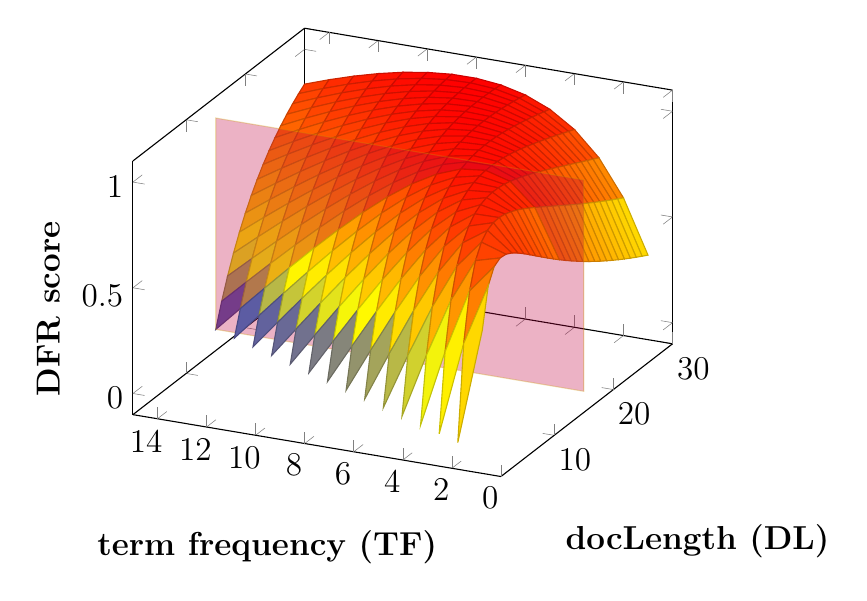
\begin{tikzpicture}[thick,scale=1.0, every node/.style={transform shape}]\begin{axis}[
 %title={},
% y dir=reverse, 
 x dir=reverse, 
 ylabel={docLength (DL)},
 xlabel={term frequency (TF)},
 zlabel={DFR score},
 every axis/.append style={font=\large\bfseries},
 max space between ticks=25pt
% yticklabels={0k,100k}
 ] 


\addplot3[surf,unbounded coords=jump]
coordinates  { 
(1,15,0.602828690204566)	(2,15,0.830458458727289)	(3,15,0.934450716638443)	(4,15,0.966903402267895)	(5,15,0.953929912325151)	(6,15,0.910204250164967)	(7,15,0.844773148573639)	(8,15,0.763616521737829)	(9,15,0.670903438148194)	(10,15,0.569664557459257)	(11,15,0.462178197338477)	(12,15,0.350204856834806)	(13,15,0.235136442615999)	(14,15,0.11809496699829)	(15,15,0)

(1,16,0.578099188538087)	(2,16,0.811155500645937)	(3,16,0.92455241464552)	(4,16,0.967767908505993)	(5,16,0.966062841257201)	(6,16,0.933720545287019)	(7,16,0.87957150961847)	(8,16,0.809460625419414)	(9,16,0.72746535973258)	(10,16,0.636550382771426)	(11,16,0.538944280996693)	(12,16,0.436368745300519)	(13,16,0.330184550451496)	(14,16,0.221488171413441)	(15,16,0.111177842268355)

(1,17,0.554089938092192)	(2,17,0.791526910417312)	(3,17,0.913056948252712)	(4,17,0.965714873324416)	(5,17,0.973972028301543)	(6,17,0.951752192118292)	(7,17,0.907687908109167)	(8,17,0.847501039032133)	(9,17,0.775185911781543)	(10,17,0.693647497457941)	(11,17,0.60506951435267)	(12,17,0.51113872004729)	(13,17,0.413187919650668)	(14,17,0.312290682010694)	(15,17,0.209326130035835)

(1,18,0.530802801771364)	(2,18,0.771767857536177)	(3,18,0.900372831623677)	(4,18,0.961364141168104)	(5,18,0.978478269819011)	(6,18,0.965306243347949)	(7,18,0.930298335362267)	(8,18,0.879063614353843)	(9,18,0.815520463917971)	(10,18,0.742519493293841)	(11,18,0.662203670865781)	(12,18,0.576228097258246)	(13,18,0.485900278395978)	(14,18,0.392273096789813)	(15,18,0.296208439454882)

(1,19,0.508226789640423)	(2,19,0.752018863072771)	(3,19,0.886810317359786)	(4,19,0.955195710616974)	(5,19,0.980224486964259)	(6,19,0.975178213356986)	(7,19,0.948338450288501)	(8,19,0.905210288059222)	(9,19,0.849642347853426)	(10,19,0.784435449978092)	(11,19,0.711695334773675)	(12,19,0.633048243551952)	(13,19,0.549778660548279)	(14,19,0.462920673152469)	(15,19,0.373320528862043)

(1,20,0.48634303905334)	(2,20,0.7323812008066)	(3,20,0.872607218288516)	(4,20,0.947585137098897)	(5,20,0.97971952494445)	(6,20,0.98200290254851)	(7,20,0.962559939768004)	(8,20,0.926799408296809)	(9,20,0.878505521275719)	(10,20,0.820433262364011)	(11,20,0.754654182131245)	(12,20,0.682768072499512)	(13,20,0.606038355509857)	(14,20,0.525481948969255)	(15,20,0.441930831844985)

(1,21,0.465128061580168)	(2,21,0.712927637929877)	(3,21,0.857947247761062)	(4,21,0.93882895517277)	(5,21,0.97736988612122)	(6,21,0.986291533238511)	(7,21,0.973572063624968)	(8,21,0.944530636289626)	(9,21,0.902891730766613)	(10,21,0.851367936716025)	(11,21,0.791999256676888)	(12,21,0.726361125537109)	(13,21,0.655697602410148)	(14,21,0.581009843803962)	(15,21,0.503116746944407)

(1,22,0.444555871588363)	(2,22,0.69371003859671)	(3,22,0.842973247656932)	(4,22,0.929163209859617)	(5,22,0.973503053852954)	(6,22,0.988459253367945)	(7,22,0.981872662054963)	(8,22,0.958978737875236)	(9,22,0.923446336219237)	(10,22,0.877948672683593)	(11,22,0.824496515075059)	(12,22,0.764642770856045)	(13,22,0.699613620363273)	(14,22,0.630395687626556)	(15,22,0.557795822851653)

(1,23,0.424599383032406)	(2,23,0.674764818583908)	(3,23,0.827796862032113)	(4,23,0.918777149915091)	(5,23,0.968384861977651)	(6,23,0.988845761863186)	(7,23,0.987871568720419)	(8,23,0.970619283566948)	(9,23,0.940705773382284)	(10,23,0.900767545813065)	(11,23,0.852788172693824)	(12,23,0.798299644283731)	(13,23,0.738511566834336)	(14,23,0.674397111108444)	(15,23,0.606751988315705)

(1,24,0.40523132186617)	(2,24,0.656116904788573)	(3,24,0.812505700538763)	(4,24,0.907823472234563)	(5,24,0.962232586378857)	(6,24,0.987730954630336)	(7,24,0.991908481950635)	(8,24,0.979848390893796)	(9,24,0.955118795248774)	(10,24,0.920321862204126)	(11,24,0.87741577498763)	(12,24,0.827913032165606)	(13,24,0.773007819631001)	(14,24,0.713660808324183)	(15,24,0.650657372038589)

(1,25,0.38642481493876)	(2,25,0.637782639637063)	(3,25,0.79716870357892)	(4,25,0.896426073240635)	(5,25,0.955224921679465)	(6,25,0.985346919947008)	(7,25,0.994266744020595)	(8,25,0.986998033599149)	(9,25,0.96706304333111)	(10,25,0.937031713492213)	(11,25,0.898838449553016)	(12,25,0.853977527193232)	(13,25,0.803628737708457)	(14,25,0.748741099129492)	(15,25,0.690090359300742)

(1,26,0.36815376139952)	(2,26,0.619771931399019)	(3,26,0.781840202366091)	(4,26,0.884685975052332)	(5,26,0.947509661773085)	(6,26,0.981887225781465)	(7,26,0.995184065634633)	(8,26,0.992348018723311)	(9,26,0.976858081971228)	(10,26,0.95125386482836)	(11,26,0.917447437797707)	(12,26,0.876915988605277)	(13,26,0.830825830481115)	(14,26,0.78011508458774)	(15,26,0.725550507465349)

(1,27,0.350393057325973)	(2,27,0.60208985927249)	(3,27,0.766563020474647)	(4,27,0.872685899583419)	(5,27,0.939209668327629)	(6,27,0.977514176161289)	(7,27,0.994860946200371)	(8,27,0.996135435044116)	(9,27,0.984775730704953)	(10,27,0.963292820489072)	(11,27,0.933577738074063)	(12,27,0.897091603060034)	(13,27,0.854988073305192)	(14,27,0.808195051131356)	(15,27,0.757470870504045)

(1,28,0.333118721214438)	(2,28,0.584737880102515)	(3,28,0.751370863683325)	(4,28,0.860493830168551)	(5,28,0.930427549263709)	(6,28,0.97236452885122)	(7,28,0.993467339157226)	(8,28,0.998562165131648)	(9,28,0.99104831536007)	(10,28,0.973409701227053)	(11,28,0.947517492491807)	(12,28,0.914817660899949)	(13,28,0.876451950536151)	(14,28,0.833338655534655)	(15,28,0.786228199121581)

(1,29,0.316307952698114)	(2,29,0.567714741253384)	(3,29,0.736290176025056)	(4,29,0.848165807395434)	(5,29,0.921249355632251)	(6,29,0.966554036195814)	(7,29,0.991147968519457)	(8,29,0.999800901797173)	(9,29,0.995875303197284)	(10,29,0.981829412799183)	(11,29,0.959515600327343)	(12,29,0.930365523362214)	(13,29,0.89550968334361)	(14,29,0.855857318363783)	(15,29,0.81215140336571)

(1,30,0.299939146627551)	(2,30,0.55101717484961)	(3,30,0.721341591745516)	(4,30,0.835748140323265)	(5,30,0.911747524748403)	(6,30,0.960181077894388)	(7,30,0.988026599941357)	(8,30,1)	(9,30,0.999428673828312)	(10,30,0.98874647076145)	(11,30,0.969787928978429)	(12,30,0.943971149900242)	(13,30,0.912416001900636)	(14,30,0.876023168107538)	(15,30,0.835528594560206)

};

\addplot3 [data cs=cart,surf,domain=-10:10,samples=2, opacity=0.3,color=purple] coordinates  { 
(0,15,0) (0,15,1)

(15,15,0) (15,15,1)

};


\addplot3[surf,unbounded coords=jump]
coordinates  { 
%patch,patch type=biquadratic, shader=faceted,patch refines=3
(1,1,0)	(2,1,nan)	(3,1,nan)	(4,1,nan)	(5,1,nan)	(6,1,nan)	(7,1,nan)	(8,1,nan)	(9,1,nan)	(10,1,nan)	(11,1,nan)	(12,1,nan)	(13,1,nan)	(14,1,nan)	(15,1,nan)

(1,2,0.550946811011921)	(2,2,0)	(3,2,nan)	(4,2,nan)	(5,2,nan)	(6,2,nan)	(7,2,nan)	(8,2,nan)	(9,2,nan)	(10,2,nan)	(11,2,nan)	(12,2,nan)	(13,2,nan)	(14,2,nan)	(15,2,nan)

(1,3,0.739499035509737)	(2,3,0.447402531994322)	(3,3,0)	(4,3,nan)	(5,3,nan)	(6,3,nan)	(7,3,nan)	(8,3,nan)	(9,3,nan)	(10,3,nan)	(11,3,nan)	(12,3,nan)	(13,3,nan)	(14,3,nan)	(15,3,nan)

(1,4,0.808372355369359)	(2,4,0.674021740218476)	(3,4,0.367084989657738)	(4,4,0)	(5,4,nan)	(6,4,nan)	(7,4,nan)	(8,4,nan)	(9,4,nan)	(10,4,nan)	(11,4,nan)	(12,4,nan)	(13,4,nan)	(14,4,nan)	(15,4,nan)

(1,5,0.827712304044469)	(2,5,0.795475244633043)	(3,5,0.589020399660793)	(4,5,0.309402318963368)	(5,5,0)	(6,5,nan)	(7,5,nan)	(8,5,nan)	(9,5,nan)	(10,5,nan)	(11,5,nan)	(12,5,nan)	(13,5,nan)	(14,5,nan)	(15,5,nan)

(1,6,0.823758030119902)	(2,6,0.861291472386904)	(3,6,0.728208149339069)	(4,6,0.516703283500178)	(5,6,0.266826414784725)	(6,6,0)	(7,6,nan)	(8,6,nan)	(9,6,nan)	(10,6,nan)	(11,6,nan)	(12,6,nan)	(13,6,nan)	(14,6,nan)	(15,6,nan)

(1,7,0.808049149749894)	(2,7,0.895286730204683)	(3,7,0.81731608309985)	(4,7,0.659114482699154)	(5,7,0.458088606324659)	(6,7,0.234329891272407)	(7,7,0)	(8,7,nan)	(9,7,nan)	(10,7,nan)	(11,7,nan)	(12,7,nan)	(13,7,nan)	(14,7,nan)	(15,7,nan)

(1,8,0.786232834510155)	(2,8,0.910031065751261)	(3,8,0.874547067067584)	(4,8,0.758685635473427)	(5,8,0.597677806310571)	(6,8,0.410536626837436)	(7,8,0.208787788218013)	(8,8,0)	(9,8,nan)	(10,8,nan)	(11,8,nan)	(12,8,nan)	(13,8,nan)	(14,8,nan)	(15,8,nan)

(1,9,0.761283776662586)	(2,9,0.912649127410629)	(3,9,0.9106548363097)	(4,9,0.828974496924382)	(5,9,0.700999123980372)	(6,9,0.54484240060699)	(7,9,0.371505245812937)	(8,9,0.188214411477962)	(9,9,0)	(10,9,nan)	(11,9,nan)	(12,9,nan)	(13,9,nan)	(14,9,nan)	(15,9,nan)

(1,10,0.734851414275236)	(2,10,0.907408307407578)	(3,10,0.932312475346719)	(4,10,0.878648510130617)	(5,10,0.778218625288615)	(6,10,0.648369486864792)	(7,10,0.499658763815525)	(8,10,0.339026534140879)	(9,10,0.171302777785929)	(10,10,0)	(11,10,nan)	(12,10,nan)	(13,10,nan)	(14,10,nan)	(15,10,nan)

(1,11,0.707882534208275)	(2,11,0.896978134982265)	(3,11,0.943832686982997)	(4,11,0.91344706582647)	(5,11,0.83622890765175)	(6,11,0.728859016655641)	(7,11,0.601513634159584)	(8,11,0.460887857152159)	(9,11,0.311641587291567)	(10,11,0.157162472776661)	(11,11,0)	(12,11,nan)	(13,11,nan)	(14,11,nan)	(15,11,nan)

(1,12,0.680931777320597)	(2,12,0.883087512447978)	(3,12,0.948098319824685)	(4,12,0.937288690029642)	(5,12,0.879825806210446)	(6,12,0.791804036576653)	(7,12,0.683066380350784)	(8,12,0.560095278476284)	(9,12,0.427403757686762)	(10,12,0.288272090676837)	(11,12,0.145167857760471)	(12,12,0)	(13,12,nan)	(14,12,nan)	(15,12,nan)

(1,13,0.654326072191879)	(2,13,0.866887863527846)	(3,13,0.947091556647468)	(4,13,0.95292023017884)	(5,13,0.912425568445965)	(6,13,0.841179268774445)	(7,13,0.748729504809226)	(8,13,0.641371703296107)	(9,13,0.523490353484945)	(10,13,0.398272129069081)	(11,13,0.268113442610775)	(12,13,0.134867288166317)	(13,13,0)	(14,13,nan)	(15,13,nan)

(1,14,0.628256015834611)	(2,14,0.849163506028517)	(3,14,0.942208095803169)	(4,14,0.962311537733073)	(5,14,0.936513154948686)	(6,14,0.879914128436669)	(7,14,0.80179902209063)	(8,14,0.708296983893924)	(9,14,0.603678740961905)	(10,14,0.491048437946633)	(11,14,0.372739929982426)	(12,14,0.25055715796921)	(13,14,0.125926946814904)	(14,14,0)	(15,14,nan)

(1,15,0.602828690204566)	(2,15,0.830458458727289)	(3,15,0.934450716638443)	(4,15,0.966903402267895)	(5,15,0.953929912325151)	(6,15,0.910204250164967)	(7,15,0.844773148573639)	(8,15,0.763616521737829)	(9,15,0.670903438148194)	(10,15,0.569664557459257)	(11,15,0.462178197338477)	(12,15,0.350204856834806)	(13,15,0.235136442615999)	(14,15,0.11809496699829)	(15,15,0)

};


 \end{axis} \end{tikzpicture}

	\label{dfrTFDLcomp}
\end{figure} 

Similarly to previous sections, we simulated the scores produced by DFRee given a range of TF and DL values with the objective of studying its behaviour in microbloging conditions. The simulated values are shown in Figure \ref{dfrTFDLcomp}.

As we traverse the Document Length axis we can observe an interesting behaviour. For low values of TF, incrementing DL values from 1 to approximately 16 results in a growing score. This behaviour aligns with the scope hypotheses as longer documents are regarded as more informative. However, for values of DL higher than 16 the scores experience a slow decline. The latter behaviour is in line with the verbose hypotheses which assumes the extra length is due to superfluous information, when the extended length is not accompanied by higher query term frequencies.

When dealing with documents as short as microblogs it is very difficult assert their informativeness or relevance in terms of the verbose or scope hypotheses. In fact all retrieval models studied so far in this work follow them to some degree and perform worse than a simply using IDF as a retrieval model. The premises in which they are built seem to fail to effectively measure the informativeness of microblog documents. However DFRee is an interesting exception as it seems to capture the relevance of microblog documents better than any of the previously studied retrieval models, and it consistently outperforms them in almost all cases (Table \ref{traditional}).

We believe that the \textit{saturation point} behaviour observed in Figure \ref{dfrTFDLcomp} both in terms of TF and DL is responsible for DFRee outperforming other retrieval models in this task. The behaviour can be summarised as a dependency of TF and DL. In other words, the score of a document can only be higher if both TF and DL increase. Thus, incrementing the value of a single component will increase the score to a saturation point after which the score will decrease. This saturation point is given by the relationship between TF and DL. As an example, consider an average microblog document of length 15 (blue square in Figure \ref{dfrTFDLcomp}), the score is maximised when TF approaches 3, after which higher TF values result in a significant reduction to the score. As a side note, this is a very effective way of getting rid of uninformative documents such as spam in microblogs. Furthermore, consider the values of DL for TF=2 in Figure \ref{dfrTFDLcomp}. The scores grow as the values for DL approach $\simeq 9$, after which it follows a slow descent. This behaviour does not completely match the premise which assumes users will attempt to encode their messages within the character limit, therefore longer should be more informative. However the score differences in the descent are very small and may not adversely affect the results significantly.

The opposite behaviour can be observed in previous retrieval models HLM and DLM. These retrieval models consider that the longer the document the less relevant they are under microblog conditions. This behaviour goes against a basic idea of microblog writing as users try to encode as much information as possible into the character limit. 
Moreover, the behaviour of HLM and DLM exhibits a positive correlation between TF and the score produced, thus the higher the TF the higher the score. However it is important to note under this premise that a document containing only of query terms would be valued over others with richer, and more informative content. This behaviour is obviously problematic as it promotes uninformative documents, particularly spam.

Summarising, we believe that DFRee's behaviour is key to understand how to achieve the best possible results for a retrieval model under microblog conditions. Particularly important is the \textit{saturation point} behaviour as a function of TF and DL. This mechanism ensures no over/under estimations of the value of microblog documents when TF is disproportionately high with respect to DL and vice-versa.

%DFRee behaves in a different way which better models the relevance of microblog documents. As previously stated DFRee promotes longer documents up to a maximum point, which is conditioned by the values of TF and viceversa. This can be easily observed in Figure \ref{dfrTFDLcomp} for DL values under 4, as the increment of TF over 1 only decreases the retrieval model score. On the contrary given a TF of 2 or 3, a document is increasingly interesting up until a DL value of 10.

%Finally, if we consider the scores produced around the $DL=15$ area, we can see that the differences are quite subtle compared to other areas of the Figure \ref{dfrTFDLcomp}, and particularly along the DL axis. This is a good property since the value of documents should not be greatly affected when the differences in length are so small.

%If an important query term appears in a document twice, and another document once together with another term, the second document should be more important. However, this may not be true if the score differences are so great.

%
%In this section we have evidenced some of the problems faced by popular retrieval models when dealing with microblog documents. In the following section we will propose a different theory to understand the relevance on microblog documents.
\section{Towards a microblog retrieval model}
In this section firstly we further extend our experimentation on the above-mentioned retrieval models. Secondly we gather all our findings to produce a retrieval model specifically tailored to microblog retrieval.

\subsection{Score differences and Harmonisation}
So far we have introduced a set of representative retrieval models, and discussed how they behave when facing microblog-like conditions. We have mainly done so by simulating the scores produced by each model, when fixing all parameters except TF and DL which are the variables to be considered. In the above-mentioned experiments, we have observed a very interesting relationship between TF, DL and the score given to the terms. In most retrieval models performance seems to increase when we overestimate the values of TF and DL, thus forcing the models into an area of values where the score differences with respect to TF and DL are much lower.


Table \ref{stdevharmonising} holds a summary of the results for all retrieval models in their various configurations with respect to Precision@30. Additionally the third column holds the standard deviation of the simulated scores produced by the retrieval models. As it can be easily observed that the possible document scores are much closer together for those configurations that improve a retrieval model's performance. In fact there seems to be a strong negative statistical correlation between the standard deviation and the performance achieved by the retrieval models.

In other words, reducing the standard deviation of the possible scores for most of the retrieval models is connected with significantly better performance. These observations motivate the following hypothesis:\\

\textbf{\textquotedblleft The range of scores produced by retrieval models when ranking microblogs can be unfairly different due to the retrieval model's behaviour with respect to scarce TF and DL values\textquotedblright}.\\



\begin{table}[]
	\caption{Behaviour when harmonising score differences.}
	\centering
	\begin{tabular}{l|c|c|c} 	
		\textit{\textbf{Model}} & 
		\textit{\textbf{configuration}} & 
		\textit{\textbf{stdev}} & 
		\textit{\textbf{P@30}} 	
		\tabularnewline
		\hline
		DLM & \(c=2500\) & 0.2639 & 0.2988 \\
		DLM & \(c=50\) & 0.2479 & 0.4099 \\
		DLM & \(c=20\) & 0.2384 & 0.4241 \\
		\hline	
		HLM & \(c=0.15\) & 0.2553 & 0.3475\\
		HLM & \(c=0.40\) & 0.2365 & 0.4009\\
		HLM & \(c=0.99\) & 0.1135 & 0.4492\\
		\hline
		BM25 & \(b=0.75, k=1.2\) & 0.1274 & 0.3948\\
		BM25 & \(b=0.75, k=0.7\) & 0.0927 & 0.4399\\
		BM25 & \(b=0.9, k=0.1\) & 0.0181 & 0.4580\\
		\hline
		DFRee & NA & 0.2268 & 0.4614\\
		\hline
		\hline    
		PEARSON & \multicolumn{2}{|c}{-0.70 or -0.58}    \\
		KTau & \multicolumn{2}{|c}{-0.66 or -0.5555}    \\
	\end{tabular}
	\label{stdevharmonising}
\end{table}

If this hypothesis is true, we should be able to achieve similar results using a different technique to reduce the standard deviation of the scores produced by the different retrieval models. To this end we produced the results in Table \ref{loggedRMS}. This Table holds performance metrics for all retrieval models with their standard configurations, however each of the scores computed for each document have been normalised using a logarithm base 2.

As an example, the formulation for HLM would look as follows: 

\begin{small}
	\begin{align}
	\label{hlmformulalog}
	\text{HLM}(D,Q) &=  \sum_{i=1}^{n} log_2 \left[ \log_2 \left[ 1 + \frac{c \cdot f(q_i, D) \cdot ntoks }{ (1-c) \cdot f(q_i, C) \cdot |D|} \right] \right]
	\end{align}
\end{small}

As we can observe in Table \ref{loggedRMS} the results for DLM, HLM and BM25 are significantly better than standard (Table \ref{stdevharmonising}), whereas DFRee performs marginally worse than its default form and IDF remains unaffected. 

We can conclude that based on the empirical evidence presented in this work, most retrieval models are not prepared to effectively capture the relevance of microblogs. The verbose and scope hypotheses, which serves as inspiration to most retrieval models, do not hold for microblog documents. Additionally, the main reason points to their over-sensitiveness to low values of term frequency and document length. This sensitiveness often produces a high degree of score differences amongst the ranked documents which ultimately negatively affects performance.

\begin{table}[]
	
	\caption{Retrieval models performance with log-smoothed scores (All collections)} 
	\centering
	\begin{tabular}{l|c|c|c|} 
		
%		\cline{2- 6}
		\multicolumn{1}{c}{}&\multicolumn{3}{|c|}{Precision @ 30} \\ 
		\cline{2- 4}
		
			& Default & $log_2(Ret. Model)$ & \% difference \\
		\hline
					 
		$DLM$ & 0.2988 & 0.3977 & +33.10\% \\
		$HLM$ & 0.3475 & 0.4489 & +29.18\%\\
		$BM25$ & 0.3948 & 0.4336 & +9.83\%\\
		$DFRee$ & 0.4614 & 0.4531 & -1.80\%\\
		$IDF$ & 0.4626 & 0.4626 & 0\%\\
		\hline
	\end{tabular}
	\label{loggedRMS}
\end{table}

%
%\subsection{Conclusions about retrieval models}
%
%RM and us do not understand microblogs. In the following chapters we will try and develop this understanding.
%

\subsection{MBRM: A Microblogs Retrieval Model}

In previous sections, we have presented a number of problems faced by retrieval models when dealing with microblogs. We have shown empirical evidence of their existence by improving the performance of state of the art retrieval models. However we can further investigate these issues by devising a retrieval model, which relies on what we have learnt so far about microblogs. To this end, we would like to introduce a ``MicroBlogs Retrieval Model'', namely MBRM.

MBRM is made up of two main components which deal with document based information attached to an IDF component which represents the collection's information. Similarly to the formulation of BM25, the two main components of MBRM deal with document length and query term frequency. In fact we came up with a formulation to represent the behaviour we observed as being the best for microblog retrieval. The first component deals with the document length and is given by by the following logistic distribution:

\begin{equation}
DLComp(DL)={\frac  {c_1}{1+{a_1\mathrm  e}^{{-b_1DL}}}}
\end{equation}

where \(a_1, b_1\) and \(c_1\) are parameters to control the growth, maximum and starting point of the distribution. Secondly, the following component given by a gaussian distribution deals with the effect of TF over the final score produced by MBRM:

\begin{equation}
TFComp\left(TF\right)=a_2e^{-{\frac {(TF-b_2)^{2}}{2c_2^{2}}}}
\end{equation}

where \(a_2, b_2\) and \(c_2\) are parameters similar parameters to those found in the previous function. These functions were chosen as they offer good control over the curves, and their values can be bound between 1 and 0 so we do not need to normalise values when combining them. The final formulation for MBRM is given by: 

\begin{equation}
MBRM(D,Q) = \sum_{i=1}^{|Q|} (1-\alpha)*\text{IDF}(q_i) + \alpha * DLComp(|D|) * TFComp(q_i)
\end{equation}

which can be also expressed as:

\begin{equation}
MBRM(D,Q) = \sum_{i=1}^{|Q|} (1-\alpha)*\text{IDF}(q_i) + \alpha * \left({\frac  {c_1}{1+{a_1\mathrm e}^{{-b_1DL(|D|)}}}} \right) * \left(a_2e^{-{\frac {(TF(q_i)-b_2)^{2}}{2c_2^{2}}}}\right) 
\end{equation}

\begin{table}[]
	\caption{MBRM recommended parameter settings} 
	\centering
	\begin{tabular}{l|c} 	
		\hline
		\textbf{Parameter} & \textbf{Recommended values} \\
		\hline
		\centering					 
		$a_1$ & 1.5 \\
		$b_1$ & 0.3 \\
		$c_1$ & 1.0 \\
		\hline
		$a_2$ & 1.0 \\
		$b_2$ & 2.0 \\
		$c_2$ & 6.0 \\
		\hline
	\end{tabular}
	\label{recommended settings}
\end{table}

Figure \ref{microblogRM} shows a simulation of the behaviour of MBRM in terms of TF and DL. The parameters used to for both components (DLComp and TFComp) are shown in Table \ref{recommended settings}. In Figure \ref{microblogRM} we can observe how the values obtained on the TF axis decrease slowly for the initial values of TF, but rapidly accelerate in their descent to then settle near 0. This behaviour is similar to that of DFRee in which the highest importance is given to TF when near the average ~2 and then it is reduced as it increases. High TF values are most likely than not associated with spam or unimportant documents, since actual users struggling to fit their content in the 140 characters limit are unlikely to repeat words. Although this is not always the case, thus the slow descent for low values of TF.


\begin{figure}
	\centering
	\caption{MBRM: A Microblog Retrieval Model}
	%!TEX root = ./JournalChapter1.tex
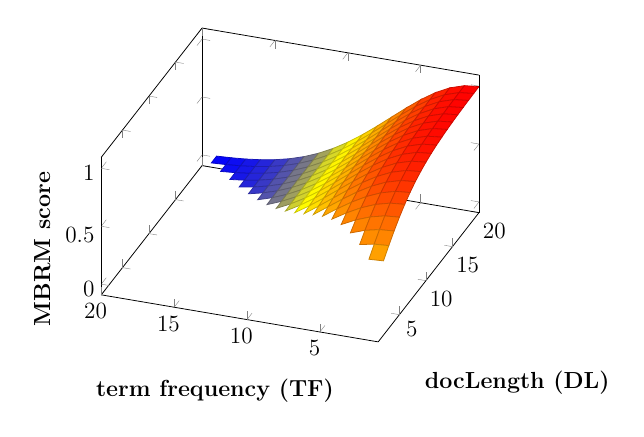
\begin{tikzpicture}[thick,scale=0.70, every node/.style={transform shape}]\begin{axis}[
 %title={},
% y dir=reverse, 
 x dir=reverse, 
 ylabel={docLength (DL)},
 xlabel={term frequency (TF)},
 zlabel={MBRM score},
 every axis/.append style={font=\large\bfseries},
  max space between ticks=25pt,
  view={20}{45}
% yticklabels={0k,100k}
 ] 

\addplot3[surf,unbounded coords=jump]
coordinates  { 
%patch,patch type=biquadratic, shader=faceted,patch refines=3
(1,1,0.473658084609043)	(2,1,nan)	(3,1,nan)	(4,1,nan)	(5,1,nan)	(6,1,nan)	(7,1,nan)	(8,1,nan)	(9,1,nan)	(10,1,nan)	(11,1,nan)	(12,1,nan)	(13,1,nan)	(14,1,nan)	(15,1,nan)	(16,1,nan)	(17,1,nan)	(18,1,nan)	(19,1,nan)	(20,1,nan)

(1,2,0.548480827396313)	(2,2,0.540915700429286)	(3,2,nan)	(4,2,nan)	(5,2,nan)	(6,2,nan)	(7,2,nan)	(8,2,nan)	(9,2,nan)	(10,2,nan)	(11,2,nan)	(12,2,nan)	(13,2,nan)	(14,2,nan)	(15,2,nan)	(16,2,nan)	(17,2,nan)	(18,2,nan)	(19,2,nan)	(20,2,nan)

(1,3,0.621174011140144)	(2,3,0.612606236245987)	(3,3,0.587605459635394)	(4,3,nan)	(5,3,nan)	(6,3,nan)	(7,3,nan)	(8,3,nan)	(9,3,nan)	(10,3,nan)	(11,3,nan)	(12,3,nan)	(13,3,nan)	(14,3,nan)	(15,3,nan)	(16,3,nan)	(17,3,nan)	(18,3,nan)	(19,3,nan)	(20,3,nan)

(1,4,0.688804056409613)	(2,4,0.679303468819562)	(3,4,0.651580743731372)	(4,4,0.607867497379652)	(5,4,nan)	(6,4,nan)	(7,4,nan)	(8,4,nan)	(9,4,nan)	(10,4,nan)	(11,4,nan)	(12,4,nan)	(13,4,nan)	(14,4,nan)	(15,4,nan)	(16,4,nan)	(17,4,nan)	(18,4,nan)	(19,4,nan)	(20,4,nan)

(1,5,0.749234519496894)	(2,5,0.738900422141148)	(3,5,0.70874551463543)	(4,5,0.661197198359976)	(5,5,0.599940192995648)	(6,5,nan)	(7,5,nan)	(8,5,nan)	(9,5,nan)	(10,5,nan)	(11,5,nan)	(12,5,nan)	(13,5,nan)	(14,5,nan)	(15,5,nan)	(16,5,nan)	(17,5,nan)	(18,5,nan)	(19,5,nan)	(20,5,nan)

(1,6,0.801315033266165)	(2,6,0.790262595943928)	(3,6,0.758011571622054)	(4,6,0.707158094310837)	(5,6,0.641643014567497)	(6,6,0.56624802053189)	(7,6,nan)	(8,6,nan)	(9,6,nan)	(10,6,nan)	(11,6,nan)	(12,6,nan)	(13,6,nan)	(14,6,nan)	(15,6,nan)	(16,6,nan)	(17,6,nan)	(18,6,nan)	(19,6,nan)	(20,6,nan)

(1,7,0.844819426554692)	(2,7,0.833166938615529)	(3,7,0.799164965930266)	(4,7,0.745550589864886)	(5,7,0.676478614671992)	(6,7,0.596990332308645)	(7,7,0.512409056462909)	(8,7,nan)	(9,7,nan)	(10,7,nan)	(11,7,nan)	(12,7,nan)	(13,7,nan)	(14,7,nan)	(15,7,nan)	(16,7,nan)	(17,7,nan)	(18,7,nan)	(19,7,nan)	(20,7,nan)

(1,8,0.880221911285893)	(2,8,0.86808112133404)	(3,8,0.832654282836054)	(4,8,0.776793175610896)	(5,8,0.704826712589884)	(6,8,0.622007443018828)	(7,8,0.533881756104225)	(8,8,0.445687908263982)	(9,8,nan)	(10,8,nan)	(11,8,nan)	(12,8,nan)	(13,8,nan)	(14,8,nan)	(15,8,nan)	(16,8,nan)	(17,8,nan)	(18,8,nan)	(19,8,nan)	(20,8,nan)

(1,9,0.908423257476761)	(2,9,0.895893489909067)	(3,9,0.859331614298145)	(4,9,0.801680778365641)	(5,9,0.727408588673019)	(6,9,0.641935880392358)	(7,9,0.550986742967013)	(8,9,0.459967260814607)	(9,9,0.373464189430496)	(10,9,nan)	(11,9,nan)	(12,9,nan)	(13,9,nan)	(14,9,nan)	(15,9,nan)	(16,9,nan)	(17,9,nan)	(18,9,nan)	(19,9,nan)	(20,9,nan)

(1,10,0.930508894824686)	(2,10,0.917674502842903)	(3,10,0.880223732854985)	(4,10,0.821171286555585)	(5,10,0.745093387208254)	(6,10,0.657542661634779)	(7,10,0.564382363663124)	(8,10,0.471150010739445)	(9,10,0.382543871816776)	(10,10,0.302092237207199)	(11,10,nan)	(12,10,nan)	(13,10,nan)	(14,10,nan)	(15,10,nan)	(16,10,nan)	(17,10,nan)	(18,10,nan)	(19,10,nan)	(20,10,nan)

(1,11,0.947575504683797)	(2,11,0.934505715101894)	(3,11,0.896368054656656)	(4,11,0.836232518160242)	(5,11,0.758759262106185)	(6,11,0.669602754917344)	(7,11,0.574733789281485)	(8,11,0.479791447122406)	(9,11,0.389560169082285)	(10,11,0.307632958400254)	(11,11,0.236280265818511)	(12,11,nan)	(13,11,nan)	(14,11,nan)	(15,11,nan)	(16,11,nan)	(17,11,nan)	(18,11,nan)	(19,11,nan)	(20,11,nan)

(1,12,0.960628005176078)	(2,12,0.947378184098945)	(3,12,0.908715191551647)	(4,12,0.847751310384182)	(5,12,0.769210889014237)	(6,12,0.678826284066198)	(7,12,0.582650533678577)	(8,12,0.486400396033392)	(9,12,0.394926215664944)	(10,12,0.311870488096952)	(11,12,0.239534938686972)	(12,12,0.178936826240635)	(13,12,nan)	(14,12,nan)	(15,12,nan)	(16,12,nan)	(17,12,nan)	(18,12,nan)	(19,12,nan)	(20,12,nan)

(1,13,0.970531794728468)	(2,13,0.957145371929495)	(3,13,0.91808377540689)	(4,13,0.856491374722895)	(5,13,0.777141224924866)	(6,13,0.685824781532228)	(7,13,0.58865748770974)	(8,13,0.491415039719145)	(9,13,0.398997787706975)	(10,13,0.315085780244454)	(11,13,0.242004472794262)	(12,13,0.180781611798323)	(13,13,0.13134737203193)	(14,13,nan)	(15,13,nan)	(16,13,nan)	(17,13,nan)	(18,13,nan)	(19,13,nan)	(20,13,nan)

(1,14,0.978001395270939)	(2,14,0.964511945212535)	(3,14,0.925149715033043)	(4,14,0.863083274619427)	(5,14,0.783122414358129)	(6,14,0.691103163124669)	(7,14,0.593188030978296)	(8,14,0.495197166247305)	(9,14,0.402068634131264)	(10,14,0.317510806325848)	(11,14,0.243867035928292)	(12,14,0.182172979327849)	(13,14,0.132358273896981)	(14,14,0.0935307681545622)	(15,14,nan)	(16,14,nan)	(17,14,nan)	(18,14,nan)	(19,14,nan)	(20,14,nan)

(1,15,0.983609577303426)	(2,15,0.97004277429664)	(3,15,0.930454828128277)	(4,15,0.868032478308364)	(5,15,0.787613096145167)	(6,15,0.69506617622544)	(7,15,0.596589566470275)	(8,15,0.498036789854914)	(9,15,0.404374228070767)	(10,15,0.319331517837884)	(11,15,0.245265449811771)	(12,15,0.183217619176433)	(13,15,0.133117259821857)	(14,15,0.094067104376561)	(15,15,0.0646513286328791)	(16,15,nan)	(17,15,nan)	(18,15,nan)	(19,15,nan)	(20,15,nan)

(1,16,0.987805871939086)	(2,16,0.974181189968945)	(3,16,0.934424352921542)	(4,16,0.871735695638039)	(5,16,0.790973226715866)	(6,16,0.698031481295689)	(7,16,0.599134748680002)	(8,16,0.500161524259554)	(9,16,0.406099377401566)	(10,16,0.320693856276042)	(11,16,0.2463118061254)	(12,16,0.183999265807626)	(13,16,0.133685167308927)	(14,16,0.0944684153180115)	(15,16,0.0649271454099729)	(16,16,0.043401252259261)	(17,16,nan)	(18,16,nan)	(19,16,nan)	(20,16,nan)

(1,17,0.990937724657488)	(2,17,0.977269845437283)	(3,17,0.937386958766447)	(4,17,0.874499546193769)	(5,17,0.793481018702778)	(6,17,0.700244600142548)	(7,17,0.601034314014291)	(8,17,0.501747293562906)	(9,17,0.407386921315999)	(10,17,0.321710620757894)	(11,17,0.247092741247879)	(12,17,0.184582638125177)	(13,17,0.134109018053835)	(14,17,0.0947679287869243)	(15,17,0.0651329978579353)	(16,17,0.0435388565535171)	(17,17,0.0283067000508986)	(18,17,nan)	(19,17,nan)	(20,17,nan)

(1,18,0.993270694323764)	(2,18,0.979570636746807)	(3,18,0.939593853595404)	(4,18,0.876558384871192)	(5,18,0.795349115053675)	(6,18,0.70189318952456)	(7,18,0.602449332120974)	(8,18,0.502928559738258)	(9,18,0.408346034392652)	(10,18,0.322468025689477)	(11,18,0.247674472930652)	(12,18,0.185017201957951)	(13,18,0.134424751589161)	(14,18,0.0949910413980342)	(15,18,0.0652863408021942)	(16,18,0.0436413603023564)	(17,18,0.0283733426571168)	(18,18,0.0179415103222197)	(19,18,nan)	(20,18,nan)

(1,19,0.995006096807971)	(2,19,0.981282103043136)	(3,19,0.94123547406905)	(4,19,0.878089872317012)	(5,19,0.79673871693961)	(6,19,0.703119508987834)	(7,19,0.603501907288596)	(8,19,0.503807256227479)	(9,19,0.409059480109465)	(10,19,0.323031428814181)	(11,19,0.248107199777478)	(12,19,0.185340456548803)	(13,19,0.134659613091851)	(14,19,0.0951570059132078)	(15,19,0.0654004064629052)	(16,19,0.043717608726392)	(17,19,0.0284229154167016)	(18,19,0.0179728570052151)	(19,19,0.0110535527433294)	(20,19,nan)

(1,20,0.996295630106907)	(2,20,0.982553849971706)	(3,20,0.942455320349234)	(4,20,0.879227881554788)	(5,20,0.797771294638723)	(6,20,0.704030755685598)	(7,20,0.604284049034176)	(8,20,0.504460193164484)	(9,20,0.409589623414655)	(10,20,0.323450079298228)	(11,20,0.248428748054262)	(12,20,0.185580658785881)	(13,20,0.134834132680887)	(14,20,0.0952803299090564)	(15,20,0.0654851657444497)	(16,20,0.0437742669844503)	(17,20,0.0284597516692636)	(18,20,0.0179961499253888)	(19,20,0.0110678782076455)	(20,20,0.0066204180310302)

};


 \end{axis} \end{tikzpicture}

	\label{microblogRM}
\end{figure} 

Now we pay attention to the values in terms of the $DL$ axis. We can observe that they increase in a soft slope as we traverse $DL$. Unlike $DFRee$, the slope is always incremental. The idea behind is that no document is significantly more important when it contains a single word more. However it should be more important since the more terms in a document the more comprehensive the document should be, particularly in terms of the amount of information encoded in it, regardless of the character limitation.


\begin{figure}
	\centering
	\caption{MBRM setting $\alpha$ per fold.}
	%
%\begin{tikzpicture}[thick,scale=0.7, every node/.style={transform shape}] \begin{axis}[
% %title={},
% %y dir=reverse, 
% %x dir=reverse, 
% ylabel={Split},
% xlabel={Alpha},
% zlabel={P@30},
% every axis/.append style={font=\large\bfseries},
% max space between ticks=25pt,
% view={-50}{20}
%% yticklabels={0k,100k}
% ] 
%
%		\addplot3[surf] coordinates { 
%%patch,patch type=biquadratic, shader=faceted,patch refines=3
%(0,1,0.4071)	(0.05,1,0.3895)	(0.1,1,0.3966)	(0.15,1,0.3975)	(0.2,1,0.3955)	(0.25,1,0.3918)	(0.3,1,0.3841)	(0.35,1,0.3751)	(0.4,1,0.3656)	(0.45,1,0.3539)	(0.5,1,0.3227)	(0.55,1,0.2764)	(0.6,1,0.2304)	(0.65,1,0.1951)	(0.7,1,0.1681)	(0.75,1,0.1434)	(0.8,1,0.1181)	(0.85,1,0.1043)	(0.9,1,0.0985)	(0.95,1,0.0905)
%
%(0,2,0.2188)	(0.05,2,0.2241)	(0.1,2,0.2322)	(0.15,2,0.2324)	(0.2,2,0.2317)	(0.25,2,0.2281)	(0.3,2,0.2275)	(0.35,2,0.2253)	(0.4,2,0.2191)	(0.45,2,0.2102)	(0.5,2,0.197)	(0.55,2,0.1859)	(0.6,2,0.1599)	(0.65,2,0.1417)	(0.7,2,0.1324)	(0.75,2,0.113)	(0.8,2,0.1025)	(0.85,2,0.0908)	(0.9,2,0.0876)	(0.95,2,0.0832)
%
%(0,3,0.1814)	(0.05,3,0.1878)	(0.1,3,0.1978)	(0.15,3,0.2)	(0.2,3,0.2014)	(0.25,3,0.2026)	(0.3,3,0.2027)	(0.35,3,0.2023)	(0.4,3,0.1993)	(0.45,3,0.193)	(0.5,3,0.1859)	(0.55,3,0.1707)	(0.6,3,0.1521)	(0.65,3,0.1322)	(0.7,3,0.1187)	(0.75,3,0.1006)	(0.8,3,0.0853)	(0.85,3,0.0748)	(0.9,3,0.0716)	(0.95,3,0.0685)
%
%(0,4,0.3427)	(0.05,4,0.3334)	(0.1,4,0.3351)	(0.15,4,0.3361)	(0.2,4,0.3366)	(0.25,4,0.3366)	(0.3,4,0.3364)	(0.35,4,0.3339)	(0.4,4,0.3273)	(0.45,4,0.315)	(0.5,4,0.2927)	(0.55,4,0.2695)	(0.6,4,0.2312)	(0.65,4,0.1978)	(0.7,4,0.1686)	(0.75,4,0.1426)	(0.8,4,0.1141)	(0.85,4,0.0998)	(0.9,4,0.0929)	(0.95,4,0.0874)
%
%(0,5,0.3696)	(0.05,5,0.382)	(0.1,5,0.3856)	(0.15,5,0.3867)	(0.2,5,0.3857)	(0.25,5,0.3833)	(0.3,5,0.379)	(0.35,5,0.3763)	(0.4,5,0.367)	(0.45,5,0.3549)	(0.5,5,0.3346)	(0.55,5,0.3068)	(0.6,5,0.2717)	(0.65,5,0.2308)	(0.7,5,0.2057)	(0.75,5,0.1727)	(0.8,5,0.1506)	(0.85,5,0.1338)	(0.9,5,0.1251)	(0.95,5,0.1178)
%
%
%}; \end{axis} \end{tikzpicture}
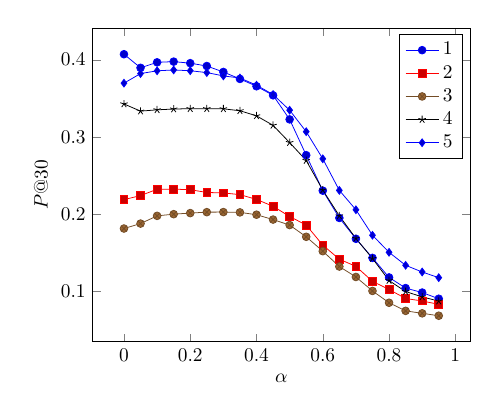
\begin{tikzpicture}[thick,scale=0.7, every node/.style={transform shape}]
\begin{axis}[
	xlabel={$\alpha$},
	ylabel={$P@30$}
]
\addplot coordinates {
	(0,0.4071)	(0.05,0.3895)	(0.1,0.3966)	(0.15,0.3975)	(0.2,0.3955)	(0.25,0.3918)	(0.3,0.3841)	(0.35,0.3751)	(0.4,0.3656)	(0.45,0.3539)	(0.5,0.3227)	(0.55,0.2764)	(0.6,0.2304)	(0.65,0.1951)	(0.7,0.1681)	(0.75,0.1434)	(0.8,0.1181)	(0.85,0.1043)	(0.9,0.0985)	(0.95,0.0905)
};

\addplot coordinates{	
	(0,0.2188)	(0.05,0.2241)	(0.1,0.2322)	(0.15,0.2324)	(0.2,0.2317)	(0.25,0.2281)	(0.3,0.2275)	(0.35,0.2253)	(0.4,0.2191)	(0.45,0.2102)	(0.5,0.197)	(0.55,0.1859)	(0.6,0.1599)	(0.65,0.1417)	(0.7,0.1324)	(0.75,0.113)	(0.8,0.1025)	(0.85,0.0908)	(0.9,0.0876)	(0.95,0.0832)
};

\addplot coordinates{
	(0,0.1814)	(0.05,0.1878)	(0.1,0.1978)	(0.15,0.2)	(0.2,0.2014)	(0.25,0.2026)	(0.3,0.2027)	(0.35,0.2023)	(0.4,0.1993)	(0.45,0.193)	(0.5,0.1859)	(0.55,0.1707)	(0.6,0.1521)	(0.65,0.1322)	(0.7,0.1187)	(0.75,0.1006)	(0.8,0.0853)	(0.85,0.0748)	(0.9,0.0716)	(0.95,0.0685)
};

\addplot coordinates{
	(0,0.3427)	(0.05,0.3334)	(0.1,0.3351)	(0.15,0.3361)	(0.2,0.3366)	(0.25,0.3366)	(0.3,0.3364)	(0.35,0.3339)	(0.4,0.3273)	(0.45,0.315)	(0.5,0.2927)	(0.55,0.2695)	(0.6,0.2312)	(0.65,0.1978)	(0.7,0.1686)	(0.75,0.1426)	(0.8,0.1141)	(0.85,0.0998)	(0.9,0.0929)	(0.95,0.0874)
};

\addplot coordinates{
		(0,0.3696)	(0.05,0.382)	(0.1,0.3856)	(0.15,0.3867)	(0.2,0.3857)	(0.25,0.3833)	(0.3,0.379)	(0.35,0.3763)	(0.4,0.367)	(0.45,0.3549)	(0.5,0.3346)	(0.55,0.3068)	(0.6,0.2717)	(0.65,0.2308)	(0.7,0.2057)	(0.75,0.1727)	(0.8,0.1506)	(0.85,0.1338)	(0.9,0.1251)	(0.95,0.1178)
};
\legend{$1$,$2$,$3$,$4$,$5$}
\end{axis}
\end{tikzpicture}
	\label{microblogRM-param}
\end{figure} 

Figure \ref{microblogRM-param} shows the results of parameter optimisation by means of a 5-fold cross-validation. The whole set of topics is subdivided into 5 groups where 4 are used for training and one for testing. The roles of each group are alternated resulting in 5 different experiments. It can very easily be observed that the most optimal values for the mixing parameter $\alpha$ are near $0.20$.


Table \ref{MBRMPerformance} shows the performance results obtained for MBRM in terms of Precision at different levels with respect to IDF and DFRee. As it can be observed, the performance is always significantly superior than the baselines. The main difference with respect to IDF is obviously that it takes advantage of document statistics, where IDF does not. However the main difference with respect to DFRee is that documents longer than 15 terms are not penalised following the aforementioned rationale. These results not only demonstrate that we can make effective use of document statistics unlike previously thought by other authors \cite{naveed2011searching}, but also that the scope hypotheses still holds for small documents. In other words, the authors of the documents will attempt to encode as much information as possible even with the obvious document limitations. This contradicts our findings in Subsection \ref{bm25case} however we believe that in the particular case of BM25, document length has a much more aggressive effect on the scores, thus resulting in a misleading behaviour.

\begin{table}[b] 	
	  	  	\centering
	  	  	\caption{Performance of MBRM on all collections (Where * $p<0.05$ and ** $p<0.01$ respectively, with respect to IDF and DFRee)} 
	  	 	\begin{tabular}{l|c|c|c|c|c} 	  	 	
	  	 	\cline{2- 6}
	  	 	\multicolumn{1}{c}{}&\multicolumn{5}{c}{Precision} \\ 
	  	 	\cline{2- 6} &
	  	 	\textit{\textbf{@5}} & 
	  	 	\textit{\textbf{@10}} & 
	  	 	\textit{\textbf{@15}} & 
	  	 	\textit{\textbf{@20}} & 
	  	 	\textit{\textbf{@30}} 
	  	 	\tabularnewline
	  	 	\hline
	 	 	 DFRee  & 0.62 & 0.57 & 0.54 & 0.51 & 0.46 \\
	 	 	 IDF  & 0.62 & 0.57 & 0.53 & 0.51 & 0.46 \\
	 	 	 \hline
 	 	 	 \hline
  	  	 	 MBRM ($\alpha=0.20$)  & \textbf{0.64*} & \textbf{0.59*} & \textbf{0.56**} & \textbf{0.53**} & \textbf{0.48*} \\
	  	  	\hline
	  	  	\end{tabular}
	  	  	\label{MBRMPerformance}	
\end{table}


The verbose hypotheses however seems not to hold, as authors are very careful to come up with specific words to effectively encode their message. Thus documents are not generally longer due to style differences, or the verbosity of the author, but it is rather a reflection of the author's capacity to encode rich information in such limited constraints. And this is what is ultimately captured by our MBRM retrieval model.


Final note, the previous experiment where we apply a logarithmic function to the scores of the retrieval models, reduce the effect of the possible values of DL. This can also be interpreted as being closer to the behaviour of MBRM where increasing DL also increases the score, which provides the best experimental results.
